\documentclass[openright]{Ilaris}
\usepackage{pdfpages}
\usepackage{verbatim}
\usepackage{fourier}
\usepackage{geometry}
%\input{kreaturen.tex}

\setlist{nolistsep, align=parleft,left=5pt..1.5em}

\renewtcolorbox{pergamentbox}[1][]{
	unbreakable,
	blankest,
	top=0.03\linewidth,
	left=0.03\linewidth,
	right=0.03\linewidth,
	bottom=0.03\linewidth,
	watermark graphics=gfx/kasten/kasten_farbe.png, 
	watermark stretch=1,
	width=\linewidth,
	#1
}

\newtcolorbox{whitebox}[1][]{
	enhanced jigsaw,
	unbreakable,
	%blankest,
	boxsep=0pt,
	%nobeforeafter,
	arc=0mm,
	outer arc=0mm
	boxrule=0mm,
	leftrule=1mm,
	rightrule=0mm,
	bottomrule=0mm,
	toprule=0mm,
	top=2mm,
	left=2mm,
	right=2mm,
	bottom=2mm,
	colframe=beige,
	width=\linewidth,
	colback=white,
	#1
}
\newcommand{\vorlesen}[1]{\begin{whitebox}#1\end{whitebox}}

% NOTE Font liegt jetzt mit im Repository. Funktionert bei mir unter Windows und Linux.
%\newfontfamily{\rog}{Rogolan.ttf}
\newfontfamily{\rog}{rogolan.otf}

\newcommand{\fkv}{Finsterkamm-Volk }
\newcommand{\fkvs}{Finsterkamm-Volks }


\newcommand{\amboss}{\hline\zeichnung{amboss.png}\\[10pt]}
\newcommand{\leer}{\hline\\[1.2cm]}
\newcommand{\linkeseite}{\begin{multicols}{3}\mbox{ }\linebreak \begin{tabularx}{1.5cm}{|X|}}
		\newcommand{\mitte}{
			\hline
		\end{tabularx}
		\neuespalte
		\begin{center}
			\usekomafont{chapter}
		}


\setdescription{itemsep=0cm} %\baselineskip
\setenumerate{itemsep=0cm} %\baselineskip

%TODO: Ggf. auf Windows-Systemen andere /\-Konvention berücksichtigen.
\graphicspath{
	%Bilder liegen in Unterordnern. Hier Windows-Codiert. Für bessere Betriebssysteme \ mit / ersetzen.
	%Je nach Ordnerstruktur müssen auch im ersten Pfad die ..\angepasst werden.
	{asche_im_wind/gfx/}
	{schwarze_hand/gfx/}
	{klamm_und_heimlich/gfx/}
	{bergkoenig/gfx/}
	{spielhilfen/gfx/}
	{res/img}%
}


\title{Die Chroniken von Ilaris\\ Band II\\ Abenteuer und Spielhilfen aus der Community}
\input{kreaturen.tex}
\begin{document}
\hauptteil
\titelseite{%
	\begin{centering}
		\titelbild{cover.jpg}
		\mbox{}
		\vspace{10cm}
		%\titel{Die Chroniken von Ilaris}
		%\\ 
		%Band II\\ Abenteuer und Spielhilfen aus der Community}
		
	%	\titel{Mockup}\\
	%	 als Diskussionsgrundlage\\ für die Arbeit an der Anthologie zum ersten Ilaris-Abenteuerwettbewerb
		
%		\platz
%		\fanprodukt
	\end{centering}
}
\neueseite
%TODO

%Neue Slogans Sephrasto
% Überschriften außerhalb von multicols zentriert?
%Spielhilfen: Beschreibung der Brauerei (ggf. mit Videos)
%Neue Illustrationen einpflegen
%Nachbesserungen der verbleibenden Autor*innen
%TODO


\subsection*{Version 0.8 vom \today}
Cover ausgetauscht

Titelgrafiken zwei Abenteuer

Goblin-Illustration ins richtige Abenteuer versetzt

Illustration von Alnus (Platzhalter)

\subsection*{Versionsgeschichte}


\subsubsection*{Version 0.7}
Titelseiten-Design vorbereitet und zwei Grafiken Bernard eingefügt

Vorwort eingefügt

Nachbesserungen \enquote{Asche}

Korrektorat Charakterbögen \enquote{Bergkönig} und Illustration von Zillie Zeh

Anhänge zum Ausdrucken ans Ende verschoben


\subsubsection*{0.6}
Inhaltsverzeichnis gekürzt

Encounter-Spielhilfe fertig layoutet und mit dem Autor abgestimmt

\enquote{Schwarze Hand} fertig layoutet

Abenteuer aus dem Bestand bebildert

Kleinere Korrekturen

%\subsubsection*{0.5}
%Encounter-Spielhilfe eingefügt und erste Hälfte layoutet
%
%Reihenfolge der Abenteuer verändert
%
%Todo-Liste für den Satz angelegt
%
%Finetuning \enquote{Schwarze Hand}
%
%Übersicht über die Spielhilfen begonnen
%
%Überarbeitung \enquote{Hallen des Bergkönigs} nach Jury-Feedback
%
%Autor*innennamen hinzugefügt
%
%IHVZ-Einträge für Charaktere, Leere Seiten aus den Charakterbögen gekürzt 
%
%Höhlenkarte (\enquote{Klamm und heimlich}) eingebunden
%
%Kleinere Korrekturen 
%
%\subsubsection*{0.4}
%Charakterbögen eingebunden
%
%IHVZ angepasst  
%
%Groblayout viertes Abenteuer 
%
%Kreaturenkästen für Klamm und heimlich

%\subsubsection*{0.3}
%Vereinheitlichung Zitation und andere Markups in den drei Abenteuern
%
%Plätze für Grafiken (vorbehaltlich Textänderungen nach Feedback)
%
%Hierarchie der Überschriften vereinheitlicht

%\subsubsection{0.2}
%Groblayout drei Abenteuer
%
%Einbau Probenkästen
%
%Interne Referenzen


%TODO: Formatierungskonventionen
%Zitatangaben kursiv und mit Doppelpunkt: \emph{Reich des roten Mondes:69}, das Regelbuch als \emph{Ilaris:9}.
%\textbf{Aventurische Begriffe}, \emph{Regelwerk-Begriffe}, \textsc{Name von Zauber oder Liturgie}.


\platz

\credit{Organisation und Redaktion}{
	\href{https://github.com/XaverStiensmeier/IlarisGlossaryEntries}{Xaver Stiensmeier}
}

\credit{Abenteuer-Autor*innen}{
	Matthias Ott\\
	Tilmann Kircher\\
	Jasmin Drogat\\
	Benjamin Drogat\\
	Matthias Thanos
	
}
\credit{Spielhilfen-Autor*innen}{	
	Arne Strehlow\\
	Alrik Normalpaktierer
	% Gatsu\\
	% Thymian\\
}
\credit{Illustrationen}{
	\href{https://www.artstation.com/bernhard\_eisner}{Bernhard Eisner}\\
	Matthias Thanos\\
	Alnus (Anton Dobsak)\\
	% Norman Obst\\
	% René Dudziak\\
	\href{https://www.zillie-zeh.de/}{Zillie Zeh}
}	
\credit{\LaTeX-Klasse}{
	\href{https://github.com/ilaris-tools/IlarisTex}{Lukas Ruhe}
}

\credit{Satz}{
	Matthias Ott\\
	Lukas Ruhe\\
	\href{https://github.com/XaverStiensmeier/IlarisGlossaryEntries}{Xaver Stiensmeier}\\
	
}
\credit{Korrektorat}{
	% Matthias Ott\\
	% Tilmann Kircher
}
%\credit{Glossar}{\href{https://github.com/XaverStiensmeier/IlarisGlossaryEntries}{Xaver Stiensmeier}}
\lizenz
\inhaltsverzeichnis
\neueseite

\kapitel{Vorwort}
\spaltenanfang
Der zweite Ilaris-Abenteuerwettbewerb im Winter 2023/2024 war ein voller Erfolg, und das verdanken wir in erster Linie den herausragenden Einsendungen, die uns erreicht haben.
Unsere Jury, bestehend aus \textbf{Niklas Bräuer} (Almanach der Abenteuer), \textbf{Sidonia von Nadoret} und \textbf{Christian Bathen} (Mistress \& Knight), \textbf{Yvonne \enquote{Schattenkatze}} (Orkenspalter) sowie mir, \textbf{Xaver Stiensmeier}, für das Ilaris-Team, hatte beim Studieren große Freude.
Um so mehr freue ich mich jetzt, dass ihr den fertigen Band in den physischen oder digitalen Händen halten könnt. Jedes einzelne Abenteuer reizt auf seine eigene Weise und auch wenn wir final eine Reihenfolge festlegen mussten, weisen alle Beiträge \textit{„Hohe Qualität“} auf (Wortspiel beabsichtigt).

Deshalb, ohne große Worte zu den Platzierungen:

\subsection*{1. Platz: In den Hallen des Bergkönigs (Matthias Ott)}
Dieses Abenteuer führt erfahrene Helden tief ins Herz der Finsterkoppen, die Heimat von Bergkönig Garbalon Sohn des Gerambalosch, dem Hochkönig des Finsterkamms, dessen Zustand auch im Mittelpunkt der Handlung steht.

Unsere Helden müssen nicht nur ihre Kampffertigkeiten, sondern auch ihren Verstand in besonders praktischer Weise einsetzen, um das Königreich vor einer drohenden Gefahr zu bewahren.
\subsection*{2. Platz: Die Schwarze Hand im Wen\-gen\-holmer Land (Tilmann Kircher)}
In diesem „hotzenplotzerischen“ Abenteuer erwartet die Helden im Wengenholmer Land eine scheinbar einfache Aufgabe, die sich als schwerer als erwartet entpuppt, und deren Auflösung eine besondere Begegnung bereithält.
\subsection*{3. Platz: Asche im Wind\newline (Jasmin \& Benjamin Drogat)}
Dieses durchaus komplexe Sandbox-Abenteuer entführt die Spieler in das Svelttal, wo ihnen je nach Charakter ein anderer geschickter Einstieg ins tatsächliche Abenteuer gegeben wird: Sie müssen die Ursache für die unheimlichen Entität finden, die die Bewohner des Svelltlandes heimsucht. \textit{Asche im Wind} erzählt sich vor allem durch scheinbar zufällige Begegnungen und webt damit eine starke Atmosphäre. 

Eine reizvolle Aufgabe für erfahrene Spielleitungen.

\neuespalte

\subsection*{4. Platz: Klamm und Heimlich (Mathias Thanos)}
In diesem auf Neueinsteiger ausgerichteten Abenteuer zieht eine orkische Entführung nahe Greifenfurt euch sofort ins Geschehen. Wer, wenn nicht ihr, kann den Knappen Alfdan aus den orkischen Klauen (Hauern?) befreien? Doch gilt auch das Gebot der Vorsicht und damit des flinken und leisen Phex, da der Feind die Übermacht hat.

\medskip

In diesem Band präsentieren wir die Abenteuer geordnet nach Einstiegsfreundlichkeit und EP-Anforderung. So soll ein einfacher Einstieg und Dranbleiben gewährleistet werden. Falls ihr Abenteuer aus „Die Chroniken von Ilaris, Band I“ noch nicht gespielt habt, lassen sich diese gut nach \textit{Die Schwarze Hand im Wengenholmer Land} positionieren.
\bigskip

\subsection*{Spielhilfen}
Der Band wird durch einen Überblick über die neusten Spielhilfen abgerundet und bringt selbst noch die geniale Spielhilfe „Encounter-Design“ von Arne Strehlow mit. Encounter-Design erklärt, wie man Kämpfe spannender und vielschichtiger gestalten kann. Durch das Kampfszenario \textit{Das Ritual der Reinigung} wird die Theorie sogleich auch in die Praxis und damit an den Spieltisch überführt.% TODO Labellink setzen

Wir freuen uns über die gesteigerte Teilnehmerzahl im Vergleich zur letzten Durchführung.
Besonders möchte ich mich bei den Sponsoren Ulisses Spiele, René Dudziak, Matthias Ott und dem Ilaris-Team bedanken, die für großartige Preise gesorgt haben. Wir konnten also auch diesmal nicht alle Preise loswerden.
Vielleicht hilfst Du uns ja beim nächsten Mal dabei!

Ein besonderer Dank gilt auch den Künstlern Bernhard Eisner, Alnus (Anton Dobsak), Zillie Zeh und Matthias Thanos, die es uns ermöglicht haben, die Abenteuer visuell ansprechend zu gestalten.
Und natürlich gebührt ein riesiges Dankeschön dem Ilaris-Team, ohne das dieses Regelwerk nie das Licht der Welt erblickt hätte:
\textbf{Lukas \enquote{Curthan} Schafzahl, Lennart Sobirey, René Dudziak} und \textbf{Julius Natrup}.

Wo ich im Vorfeld viel organisatorische Arbeit hatte, kann ich mich nun, da ich diese Zeilen schreibe ziemlich zurücklehnen. Dank \textbf{Lukas Ruhe} und \textbf{Matthias Ott}, der bereits den ersten Wettbewerb organisiert und die \enquote{Chroniken von Ilaris -- Band I} herausgegeben hat, verläuft der Satz auch diesmal reibungslos. Gemeinsam – so sage ich mal ganz hochgestochen – haben wir es geschafft, den Wettbewerb auf ein neues Niveau zu heben.

Ich freue mich schon jetzt auf den nächsten Wettbewerb und bin gespannt, welche kreativen Abenteuer uns dann erwarten.

\neueseite

\subsection*{Hinweise zur Orientierung}
Das Ilaris-Regelbuch wird im folgenden mit \emph{Ilaris} und der entsprechende Seitenzahl referenziert.

\vorlesen{Texte zum Vorlesen oder Nacherzählen sind generell durch diesen Kasten hervorgehoben.}

\kasten{Braune Kästen hingegen enthalten Hintergrund-Informationen zum besseren Verständnis.}

\info{Diese Kästen nutzen wir für Anweisungen an Sie als Spielleitung.}

\probe{Klugheit}{Probenkästen}{weisen darauf hin, dass ein Würfelwurf die Szene entscheidend verändern kann.}

\probenkasten[
bild=beeinflussung,
erfolg={Dann kann man hier lesen, was im Erfolgsfall \dots},
misserfolg={\dots und hier, was bei einem Misserfolg passiert.},
zusammenarbeit=nein,
pw=X,
farbe=rot
]{Größere Kästen}{%
	erlauben beispielsweise, mehrere Schwierigkeiten anzugeben. In so einem Fall wählt das würfelnde Gruppenmitglied die gewünschte Schwierigkeit jeweils selbst.\\
	Die Symbole geben an, ob mit einem oder drei Würfeln gewürfelt wird \emph{(Ilaris:7)} \emph{Zusammenarbeit} möglich ist, ob es sich um eine \emph{Gruppenprobe} handelt, welche \emph{Schwierigkeit} \emph{(Ilaris:8)} zu überwürfeln ist, welcher \emph{Detailgrad} anliegt und ob die Probe \emph{vergleichend} \emph{(Ilaris:9)} oder als offener Wurf gegen eine feste Schwierigkeit abgelegt wird.
}

\bigskip

Wir wünschen euch viel Spaß beim Spielen und freuen uns über Rückmeldungen und Anregungen.

\bigskip

\textsl{Xaver Stiensmeier}

\spaltenende




\kapitel{Klamm und heimlich}
\thispagestyle{empty}

\begin{center}
	\usekomafont{section}
	Ein Dungeon-Gruppenabenteuer
	
	\vfill
\zeichnung[0.8\textwidth]{cover-klamm.png}
\vfill	
	
{\href{mailto:matthias.thanos@gmx.de}{Matthias Thanos}}
	\normalfont\normalcolor\normalsize
\end{center}
	
	\credit{Lektorat}{
		Elisabeth Schmitt}
	
	\credit{Danksagung}{an alle, die an einer der vier Testrunden teilgenommen haben!}
%	
%	\credit{Titelbild \& Karte}{Matthias Thanos}

\newpage
\begin{center}

\usekomafont{section}
	
Ein Dungeon-Gruppenabenteuer - Ein Beitrag zum 2.\,Ilaris Abenteuerwettbewerb


\platz

Impressum

\normalfont

\end{center}

\credit{Text \& Kontakt}
{Matthias Thanos -- [vorname].[nachname]<ätt>gmx[Pünktchen]de}


\credit{Lektorat}{
Elisabeth Schmitt}

\credit{Danksagung}{Danke an alle, die an einer der vier Testrunden teilgenommen haben!}

%\credit{Layout \& Dokumentgenerierung}
%{Matthias Thanos\\ \url{https://brauerei.ilaris-online.de}}

\credit{Ilaris-Artwork}{\href{https://www.artstation.com/bernhard\_eisner}{Bernhard Eisner}}

\credit{Titelbild, Karte}{Matthias Thanos}

\neueseite

\spaltenanfang



\abschnitt{Überblick}
Im \textbf{Greifenfurt}er Umland erfahren die Helden von einem Ork-Überfall, bei dem der \textbf{Knappe Alfdan} entführt wurde, und nehmen die Verfolgung auf.
Die Fährte führt zu einer Klamm, wo sich die Orks eingenistet haben, um von hier aus \textbf{Gut Nebelstein} zu erobern.
Nur mit List und Geschick werden es die Helden schaffen, die Orks und ihre Handlanger zu überwinden, den \textbf{Knappen Alfdan} zu befreien und dem plötzlich auftauchenden Elitetrupp des \textbf{Ork-Schamane}n zu entkommen.
\info{
\textbf{Die Erfahrungsstufe der Helden}

Dieses Abenteuer ist für 2-4 \textit{unerfahrene Neulinge} (2000~EP) konzipiert. Falls sich die Abenteuergruppe noch nicht kennt, wird sie im Vorlesetext zusammengeführt.
}

\abschnitt{Der Weg ins Abenteuer}

\info{
\textbf{Vorlesetexte}

Den folgenden Text kannst du deiner Gruppe direkt vorlesen. Lies ihn dir im Vorfeld einmal in Ruhe durch. Trage ihn dann am Spieltisch mit lebhafter Stimme vor.
}

\vorlesen{Langsam sinkt die kalte Herbstsonne hinter das \textbf{Finsterkamm}-Gebirge und taucht das Tal um \textbf{Gut Nebelstein} in tiefe Schatten. 
	Es klang nach einem bedeutsamen Auftrag, als die alte Ritterin, \textbf{Wahntraude von Rebenich}, euch in ihre Dienste nahm:
	In die Stadt Greifenfurt solltet ihr reisen und dort der \textbf{Markgräfin} die Unterstützung anbieten, um die sie angesichts der großen Bedrohung aus dem Norden schon seit langer Zeit verzweifelt bat.
	\textbf{Wahntraude} hat daher eine Gruppe an Abenteurern auf den Weg geschickt. Ihr seid \dots}

\info{
Fordere die Personen am Spieltisch nun auf, ihre Helden mit Namen und Aussehen kurz vorzustellen!
}

\vorlesen{Ihr wart schon ein gutes Stück entlang des sich talwärts mäandernden Baches gewandert, da lief euch jedoch eine Dienerin in die Arme:
	\textbf{Treudane Degenhardt}, von Dornenbüschen zerkratzt und völlig außer Atem.
	Sie war gemeinsam mit \textbf{Alfdan}, dem Knappen von Gut Nebelstein, und dessen Mutter und Gärtnerin \textbf{Alwena} auf dem Rückweg vom Markt in Greifenberg gewesen.
	Ein Dutzend grobschlächtiger Orks hat sie überfallen, wenige Meilen von hier, und den jungen \textbf{Alfdan} samt Markterlös in die Berge gezerrt.
	
	Die fürsorgliche Ritterin wird völlig aufgelöst sein, wenn sie davon erfährt, dass ihr einziger Knappe ihren Feinden in die Hände fällt! Und das wird zweifellos geschehen, wenn ihr nichts unternehmt!}

\info{
\textbf{Gelenkte Passagen}

Wie du sicherlich bemerkt hast, haben die Helden hier nicht wirklich eine Wahl, was zu tun ist. Solche Passagen können sinnvoll sein, um das Abenteuer ohne große Umwege zu starten. Damit allen am Spieltisch sofort klar ist, dass hier keine Interaktionsmöglichkeiten bestehen, ist der Vorlesetext in der Vergangenheitsform geschrieben.
}

\vorlesen{Ihr wart also sofort zum Ort des Verbrechens geeilt, um die noch frische Fährte aufzunehmen und die Entführer einzuholen. Beim zurückgelassenen Ochsenkarren stockte euch der Atem:
	Zwischen zerschlagenen Weidenkörben und zerstreuten Äpfeln lag dort blutüberströmt eine Frau, deren noch zitternde Hand auf etwas in der Ferne zu deuten schien.
	Mit letzter Kraft hauchte sie euch entgegen: „Sie haben \dots\ mein Sohn \dots“
	Da nicht mehr aus ihr herauszubekommen war, als Boron sie zu sich nahm, folgten eure Blicke ihrer nun toten Hand:
	Sie zeigte auf die Hänge des \textbf{Finsterkamm}s.
	Sofort seid ihr losgeeilt und eine ab und an sichtbare Fährte aus Bluttropfen führte euch immer höher ins Gebirge.
	Schließlich endete die Spur in einem dunklen Höhleneingang.}
\spaltenende
\begin{center}
\zeichnung[0.6\textwidth]{pferd.jpg}
\end{center}
\newpage

\spaltenanfang
\abschnitt{Höhleneingang}
\vorlesen{Als ihr einen vorsichtigen Blick hineinwagt, schlägt euch Verwesungsgeruch entgegen.
	Im Dämmerlicht der von außen eindringenden Abendröte könnt ihr Tierknochen erkennen, die den ganzen Boden bedecken.
	Als ihr einen Moment den Atem anhaltet, hört ihr ein Nagen.
	
Was tut ihr?}


\info{
Jetzt erfährst du, was die Gruppe hier entdecken könnte!
}

In der Höhle liegt ein toter \textbf{Ork} (aschfarbene Haut, dichte schwarze Behaarung, breite Nase, dominanter Überaugenwulst, Unterbiss mit hervorstechenden Eckzähnen, spitze Ohren), den gerade ein Schwarm Ratten abnagt.

Er wurde kürzlich von einem Schwert in den Bauch gestoßen, hat sich noch in die Höhle geschleppt und ist dann umgefallen und verblutet.
Sein rechter Arm ragt in einen großen Haufen Unrat.

Wer seine Hand freilegt, sieht, dass sich, unter dem Haufen versteckt, eine aufschiebbare hölzerne Bodenabdeckung befindet, die der Tote offenbar öffnen wollte. Diese Abdeckung ist außerdem etwas zu kurz geraten und lässt nach vorne hin eine kleine Lücke.

Bei einer Bedrohung durch Feuer fliehen einige der Ratten in den darunter liegenden Abgang (\textbf{Mine}).

\abschnitt{Mine}
\vorlesen{Ihr steigt den Abgang in die Finsternis hinab. Fast schnurgerade führt der enge Stollen in den Berg hinein. Die Gesteinswände sind feucht und glitschig. Ab und zu fällt ein dicker Wassertropfen auf euren Kopf.
	Die niedrige, tief zerfurchte Decke ist alle paar Schritt notdürftig mit frisch geschlagenen Holzpfosten abgestützt.

Mehrere hundert Meter müsst ihr bereits gelaufen sein, da hört ihr von vorne ein Krachen und Rumpeln, begleitet von einem sich schnell entfernenden, panischen Blöken.
Als ihr euch weiter traut, schlägt euch eine dicke Staubwolke entgegen. Das Tosen eines stürzenden Flusses dringt zu euch durch.

Als sich der Staub legt, erblickt ihr eine große natürliche Höhlenschlucht. Zuerst fällt euch ein monströses, menschenähnliches Ungetüm ins Auge, das in den Abgrund schaut. Um seine nackten, fettglänzenden Schultern hängt eine Kette aus Totenschädeln. Daneben befinden sich drei affenähnliche Gestalten mit rotem Fell, die gerade herumfeixen.

Die Höhle wird lediglich von einer einzelnen Öllampe erhellt, die in der Höhlenmitte an einer vier Meter langen Metallkette befestigt ist und gerade heftig schwingt.
}

\info{
\textbf{Offene Herausforderungen}

Dieser Raum stellt eine Hürde dar, die sowohl auf kämpferische als auch heimliche Weise überwunden werden kann.
Egal, welchen Ansatz deine Gruppe verfolgt:
Lasse dich darauf ein, ohne zu beraten, und spiele die Aktionen neutral und fair aus.
Beachte dabei, dass die Gegner ebenfalls alles versuchen werden, um siegreich aus einer Konfrontation hervorzugehen,
aber auch fliehen werden, wenn sie die Niederlage kommen sehen.
}

Die enge, unterirdische Klamm wird in rund zehn Metern Tiefe von einem ohrenbetäubend rauschenden Gewässer durchströmt (einem Zufluss der \textbf{Breite} bei \textbf{Gut Nebelstein}).
Die völlig ungesicherte Schlucht ist oben offen und macht den Nachthimmel sichtbar.
Diesseits des Abgrunds hat gerade ein Minentrupp, bestehend aus dem beschriebenen \textbf{Oger} (starke Blähungen, dumm, launisch, spricht wie auch alle Orks und Goblins in der Sprache der Helden mit einfachen Worten; Werte \emph{Ilaris:103}) und drei rotpelzigen \textbf{Goblin}s (mager, lispeln, unterwürfig, \emph{Ilaris:101}), ein größeres Stück freiliegendes Erz abgeschlagen.
Der Brocken hat jedoch einige benachbarte Stücke weggeschleudert und der folgende Steinschlag einen der beiden hier angebundenen, beim Überfall erbeuteten Ochsen in die Tiefe gerissen.
Der mit Spitzhacken, Eimern und Seilen ausgerüstete Trupp blickt deswegen noch gebannt auf den Abgrund.

Neben dem gaffenden Minentrupp führt eine an stabilen Pollern befestigte Hängebrücke über die Klamm, endet jedoch vor einem geschlossenen (und von innen verriegelten) hölzernen Tor (\textbf{Baracke}).
Vom um drei Meter erhöhten Standpunkt der Helden aus führt eine Strickleiter hinunter.

Auf der linken Seite kann ein hölzerner Kran Lasten zu einem höher gelegenen und von hier aus ansonsten unerreichbaren natürlichen Plateau (\textbf{Schmiede}) transportieren.
Die Last wird eingehakt und dann mithilfe einer unten angebrachten Kurbel und einem über eine Rolle laufenden Seil hochgezogen.
Ab und an dringt für Sekundenbruchteile orangefarben flackerndes Licht von der Schmiede in die Mine.

Immer dann, wenn jemand ein Wagnis unternimmt, kannst du eine Probe verlangen:
\probe{heimlichkeit}{Untertauchen (12)}{Um am Minentrupp vorbei zum Kran zu schleichen.}
\info{Die betreffende Person würfelt dazu drei zwanzigseitige Würfel (3W20), von denen nur das mittlere Ergebnis gewertet wird, und addiert ihren Probenwert (PW) von Heimlichkeit. Das Ergebnis muss den Zielwert von 12 erreichen, damit die Aktion glückt.}

\abschnitt{Schmiede}
\info{
Wende dich nun an den ersten Helden, der hochkommt!
}

\vorlesen{Als du dich der Felskante näherst, braust eine Stichflamme knapp über deinen Kopf hinweg. Du lauschst und hörst, wie sich eine krächzende Stimme die Seele aus dem Leib hustet. Von der Seite wird die Person über dir offenbar angebrüllt:
	
	„AAAH! Jetzt hast du SCHON WIEDER meine Haare angesengt! WASSER!!“ Du hörst ein Zischen, bevor das Geschimpfe weiter geht: „Ich hätte \textbf{Shurrak Windzahn} sagen sollen, dass wir dich und das Ei über der Esse hätten braten sollen, anstatt dich als Lehrling einzustellen!!“
	
	Als du über die Kante spähst, siehst du zu deiner Linken ein \textbf{Reptil} von knapp einem Meter Größe, das um Atem ringt und sich über eine in voller Glut stehende Feuerstelle beugt.
	
	Zur Rechten siehst du gerade noch einen \textbf{Zwerg} mit qualmender Glatze davonstapfen. Der Zwerg verschwindet zwischen einigen großen Fässern in einem Nebenraum und schlägt laut die Tür zu.
}

Bei dem bemitleidenswerten Lehrling handelt es sich um den tollpatschigen Meckerdrachen \textbf{Greifax} (Werte siehe \emph{Anhang, S.\,\pageref{greifax}}).
 \textbf{Greifax} beherrscht die Sprache der Helden, ist anfällig für Schmeicheleien und kann ein wertvoller Verbündeter sein, wenn die Helden ihn auf ihre Seite ziehen.
Er wird erpresst vom Ork-Schamanen (\textbf{Shurrak Windzahn}, \emph{siehe S.\,\pageref{finale}}):
Vor einigen Wochen haben die Orks das Nest von \textbf{Greifax} und seiner geliebten Meckerdrachin ausgeraubt und das einzige Ei in ihren Besitz gebracht.
Von seiner Geliebten verstoßen, hat \textbf{Greifax} die Verfolgung aufgenommen, um das noch unausgebrütete Ei zu retten.
Nun wird er vom Schamanen instrumentalisiert mit dem Versprechen, das Ei zurückzuerhalten.

Wenn die Helden oder \textbf{Greifax} zu viel Lärm machen, könnte dies den mit den Orks kollaborierenden Zwergenschmied \textbf{Duglim} (abgeschnittener Bart, paranoid, hasst Meckerdrachen, wurde von seiner erzzwergischen Sippe wegen Totschlags ausgeschlossen, Werte \emph{s. S.\,\pageref{duglim}}) aufmerksam machen.
Um sich vor den seiner Meinung nach übergriffigen Orks zu schützen, hat er seine Tür von innen verriegelt.

Die Helden müssen ihn überlisten, denn von seinem Zimmer aus ist die stählerne Bodenklappe verriegelt, die am Ende des Durchgangs über eine Strickleiter zur \textbf{Baracke} führt.
Erst wenn ein Hebel im Nebenraum umgelegt wird, wird eine Metallstange herausgezogen, die von unten die Klappe blockiert.


Die Fässer, auf denen „Kontor Bellentor, Lowangen“ eingebrannt ist, beinhalten Eisenerz, Nägel, Holzstiele oder Wasser.
Wenn man sie leert, sind sie überraschend leicht.
Alle haben wiederverschließbare Deckel, die jedoch nicht ganz wasserdicht sind.

Hinter eines der Fässer ist eine kleine, vom Zwerg gesuchte Ledertasche gefallen, in der eine Handvoll dicker Nadeln, ein zusammengeknüllter Faden und eine rostige Schere zu finden sind.

Eine seitliche Raumöffnung gibt den Blick frei zum Kran in der tiefer liegenden \textbf{Mine}.

\abschnitt{Baracke}
\vorlesen{Drei Schritt vor euch versperrt euch ein kreisrundes weißes Zelt die Sicht auf eine weiträumige Höhle. Spärliches Licht dringt zu euch herüber. In einer trockenen Einbuchtung neben euch liegen einige Felle und Lederreste aufgetürmt.
}

Das Zelt gehört dem \textbf{Ork-Schamanen} und beherbergt einen lose herumflatternden Brief (\emph{\ref{kuh_ho1}{Handout 1}}),
eine an die Zeltwand gepinnte, dahingekritzelte Höhlenkarte (\emph{\ref{kuh_ho2}{Handout 2}}) und einen kleinen improvisierten \textbf{Tairach}-Schrein mit einem Stierschädel.
		
Unter dem Schädel versteckt ist eine Schatulle mit kaputter Schließe und über 1.000 laut klimpernden Kupfer- und Eisenmünzen im Gesamtwert von rund 5~Dukaten.

\info{
\textbf{Umgang mit den Handouts}

Drucke die Handouts aus und händige sie der Gruppe aus, sobald sie das entsprechende Objekt im Spiel gefunden hat.

Die Höhlenkarte ist als Orientierungshilfe bei der Flucht im Finale gedacht.

Der Brief hingegen deutet den Storyhintergrund an und soll die Gruppe dazu anregen, über die Motivationen der Nichtspielercharaktere zu rätseln.

Dir können die vagen Informationshappen zudem dabei helfen, ein Anschlussabenteuer einzuleiten.
Mehr dazu unten unter \ref{ideen}{\enquote{Ideen für ein Folgeabenteuer}}.
}

Wenn die Helden am Zelt vorbeispähen, so entdecken sie entlang der Höhlenwand rund zwanzig leere Strohsäcke. In einem davon befinden sich ein Kurzbogen, ein Köcher mit 4~Pfeilen, darunter ein Brandpfeil, und einige bissige Bettwanzen.

Am linken Ende der Höhle bewacht ein zweiköpfiger Oger (Werte \emph{Ilaris:103}, Variante Kriegsoger) eine Holztür.
Seine zwei Köpfe \textbf{Bagmun} (misstrauisch und einigermaßen schlau, weiche Stimme) und \textbf{Ragmun} (aggressiv und einfältig, dumpfe Stimme) streiten wie ein altes Ehepaar und sind sich nur darin einig, dass sie beide gerne Menschen fressen.
Die Holztür führt zum \textbf{Verhörraum} und ist von hier mit einem massiven, sehr schweren und fies eingeklemmten Holzbalken blockiert.
Zufälligerweise können die Helden beobachten, wie ein Wachork den Verhörraum verlassen will und dazu von innen ein Klopfzeichen macht (kurz, lang, kurz, lang), woraufhin der Wachoger die Tür öffnet und danach sofort wieder verriegelt.

\kasten{
\textbf{Optionale Herausforderung}

Der Wachork heißt \textbf{Olruk} und soll für die „Befragung“ des Knappen in der Schmiede eine glühende Eisenstange besorgen.
Dabei droht er, die Helden zu entdecken.
}

Geradeaus hinter dem Zelt führt ein doppelflügliges Tor zum Orkland.
Das Tor ist jedoch von der anderen Seite verriegelt und wird von dort streng bewacht.

Eine Strickleiter hinter dem Zelt führt hoch zur \textbf{Schmiede} und daneben ein von hier mit einer Planke verbarrikadiertes einflügeliges Tor zur \textbf{Mine}.

\abschnitt{Verhörraum}
\vorlesen{Ein zehn Meter langer, schmaler und dunkler Gang führt euch zu einer nur angelehnten Holztür, aus der Licht dringt.
}

\info{
\textbf{Triggerwarnung}

Die folgende Szene thematisiert Folter. Damit soll vor dem Finale das Blut der Helden in Wallung gebracht werden. Wenn du das Gefühl hast, dass sich eine der Personen am Spieltisch dabei unwohl fühlen wird, dann überspringe den folgenden Vorlesetext.
}

\vorlesen{
Als ihr euch nähert, hört ihr einen schmerzverzerrten Schrei. Etwas Metallisches fällt zu Boden. Eine grunzige Stimme blökt: „Ich ziehe dir auch die anderen Nägel, wenn du nicht sofort verrätst, wo sich dieser verdammte Fluchttunnel befindet!!

Was, immer noch nicht?? Na warte, bis ich mit dir fertig bin \dots“
}
Durch den Türspalt kann man drei bis fünf mit \textbf{Arbach}-Säbeln bewaffnete Ork-Krieger \emph{(Ilaris:104)} beobachten. Auf dem Tisch liegt das Kurzschwert des Knappen (mit Gut-Nebelstein-Gravur auf dem Knauf).

Hauptork \textbf{Siburash Eberschrei} (Kriegshammer, Nasenring, trägt gut sichtbar einen Schlüsselbund mit dem Schlüssel zu Alfdans Ketten) und Wachork \textbf{Blorg} (Hasenscharte) verhören gerade gewaltsam den an der Wand gegenüber in Ketten gelegten Knappen \textbf{Alfdan} (dunkelblonder Bürstenschnitt, pummelig, Doppelkinn, gutmütig; aktuell kampfunfähig mit fünf Punkten Erschöpfung und nicht imstande zu gehen, Werte wie \emph{Stadtwache}, \emph{Ilaris:107}).



Auf dem Boden liegen eine blutige verbogene Zange und eine dreckige Peitsche.
Eine über dem Tisch hängende Laterne ist die einzige Lichtquelle.

Sollten die Helden es schaffen, den Knappen aus dem Verhörraum zu befreien, so beginnt das \textbf{Finale}.

\info{
\textbf{Regeln für den Kampf}

Sollte es zum Kampf kommen, bestimmst du zunächst, in welcher Reihenfolge die Beteiligten agieren können:
Wer die höhere Initiative hat, handelt zuerst.

Bei jedem Angriff wird eine vergleichende Probe fällig: Beide würfeln 1W20, wobei der Angreifer den Attackewert (AT*) der verwendeten Waffe addiert, der Verteidiger hingegen seinen Verteidigungswert (VT*). Hat der Angreifer das höhere Ergebnis erzielt, hat er getroffen und würfelt die angerichteten Trefferpunkte (TP*) aus.
Bei Gleichstand gewinnt der höhere Grundwert, andernfalls der Spieler.
Um den Kampf zu beschleunigen, kannst du für Nichtspielercharaktere auf das Würfeln verzichten und stattdessen ein mittleres Würfelergebnis von 10 annehmen.

Wenn die ausgewürftelten Trefferpunkte die Wundschwelle (WS*) des Ziels übertreffen, erhält dieses eine Wunde. Sofern die Trefferpunkte sogar ein Vielfaches der Wundschwelle übertreffen, erhält das Ziel mehrere Wunden. Wunden gelten wie Erschöpfungen als Einschränkung. Für jede Einschränkung wird unter Status ein Kreuz (Wunde) bzw. ein Strich (Erschöpfung) gemacht.

Ab der dritten Einschränkung erleidet der Charakter Wundabzüge für alle Proben, ab der fünften Einschränkung wird er kampfunfähig.
}

\spaltenende

\newpage

\spaltenanfang

\abschnitt{Finale}
Als die Helden den Verhörraum verlassen, öffnet sich in der Baracke mit einem lauten Schlag das doppelflüglige Tor zum Orkland.
Der Schamane \textbf{Shurrak Windzahn} \label{finale} (Knochenkeule, Fellüberwurf, trägt \textbf{Greifax}' Ei bei sich, spricht kehlig-brüllend, braucht militärische Erfolge, Werte siehe Anhang) betritt mit einem Trupp aus fünfzehn Ork-Kriegern \emph{(Ilaris:104)} die Baracke.

Er will sich nach der Entführung des Knappen erkundigen, aus diesem die Lage eines geheimen Fluchttunnels zu \textbf{Gut Nebelstein} herauspressen und die Burganlage dann noch in derselben Nacht überfallen.

Wenn \textbf{Shurrak} die Eindringlinge bemerkt, wird er sofort seine Krieger loshetzen und zudem die Ausgänge schließen und stärker bewachen lassen.
\info{
\textbf{Regeln für Verfolgungsjagden}

Verfolgungsjagden können als vergleichende Proben abgehandelt werden.
Beide Seiten würfeln dazu 1W20 und addieren den Probenwert (PW) von \emph{Athletik}.
Sollte einer der Beteiligten ein passendes Talent (z.\,B. Laufen) einsetzen, darf er statt des Probenwerts den Talentprobenwert PW(T) verwenden.
}

\info{
\textbf{Offener Handlungsabschnitt}

Damit die Helden gefordert werden und echte Spannung aufkommt, ist das Finale offen gelassen:
Weder ist festgelegt, ob die Helden entkommen können, noch wie sie das anstellen.

Wahrscheinlich ist, dass sie die Beine in die Hand nehmen, zur Schmiede hinaufklettern und die Strickleiter kappen.
Dort könnten sie  auf die todesmutige Idee kommen, über die nach draußen führende Wasserströmung zu fliehen.

Oder sie haben \textbf{Greifax} auf ihre Seite gezogen, der ihnen mit seinem Feuerodem Zeit zur Flucht verschaffen könnte.

Vielleicht sind die Helden bei der Rettungsaktion aber auch heimlich vorgegangen und versuchen nun, sich unbemerkt davonzuschleichen.
}

Sofern die Helden aufgegriffen werden, werden sie in Ketten gelegt und bis auf Weiteres für niedere Arbeiten in der Mine eingesetzt.

\info{
\textbf{Gescheitert, und dann?}

Falls die Helden gefasst werden, dann ist das Abenteuer nicht vorbei!
Gerade solche unerwarteten Wendungen machen euer Abenteuer  erinnerungswürdig.
Zelebriere in diesem Falle die Dramatik und nutze die Situation, wenn möglich, als Cliffhanger.
Auf diese Weise hast du direkt einen perfekten Aufhänger für dein Folgeabenteuer:
die Flucht aus den Fängen der Orks!
}

\neuespalte

Gelangen die Helden hingegen zusammen mit dem Knappen an die Oberfläche, haben sie das Abenteuer bestanden und erhalten im Gut Nebelstein von der Ritterin \textit{Wahntraude von Rebenich} (vernarbtes Gesicht, raue Stimme, Geldsorgen) zum Dank jeweils 3~Dukaten. Zudem können sie sich je 100~Abenteuerpunkte notieren und erhalten 20~Bonus-EP, falls sie Greifax als Verbündeten gewonnen haben.

\info{
\textbf{Verbündete NSCs im Rollenspiel}

Eigenständig agierende, friedlich beeinflussbare Nichtspielercharakterere wie \textbf{Greifax} können die soziale Interaktion bereichern.
Du solltest jedoch vermeiden, sie als ständige Begleiter zu verwenden, da dies den Fokus weg von den eigentlichen Helden lenkt.
Daher verabschiedet sich Greifax am Ende des Abenteuers und kann später wieder auftauchen, um sich für die Hilfe der Helden zu revanchieren.
}


\abschnitt{Ideen für ein Folgeabenteuer}
\label{ideen}
\info{Sofern deiner Spielrunde das Thema des Abenteuers gefallen hat und du daran anschließen möchtest, kannst du aus den Geschehnissen neue Abenteuer ableiten:}

Offenbar muss irgendjemand den Orks den Tipp gegeben haben, dass der Knappe gerade zu dieser Zeit auf der Straße entführt werden kann.
Die Dienerin \textbf{Treudane Degenhardt} (hässliche Warze am Kinn, sonst hübsch, spricht etwas zu schnell und abgehackt) steht im Verdacht, 
ich für die Enteignung ihrer einst landadligen Eltern revanchieren zu wollen, welche sich im vorletzten gräflichen Kleinkrieg auf die falsche Seite geschlagen hatten.

Womöglich hat sie sich zwischenzeitlich dem \textbf{Geheimbund der Schnitter} angeschlossen, der \textbf{Tairach} verehrt, und plant, im Bündnis mit den Orks \textbf{Gut Nebelstein} einzunehmen.
Denn der Bund hat erfahren, dass in der dortigen Krypta eines schwach orkblütigen Vorfahren der Ritterin ein Kriegsartefakt der Orks liegt.
Nur mithilfe von \textbf{Shurrak Windzahn} kann sie es bergen. Vielleicht befürchtet sie, dass \textbf{Alfdan} beim Überfall Verdacht geschöpft hat, taucht bei nächster Gelegenheit unter und wird schließlich vermisst.
Ein Fall für (ahnungslose!) Helden!

\abschnitt{Klarer Abschluss für One-Shots}

Falls du den Handlungsfaden hier enden lassen willst, dann ist \textbf{Treudane} noch nicht untergetaucht und hat auch ihre Aufzeichnungen zum orkischen Kriegsartefakt noch in ihrem Zimmer liegen.
Äußern die Helden einen Verdacht, werden diese Aufzeichnungen entdeckt und \textbf{Treudane} eingekerkert.


\spaltenende

\neueseite

\abschnitt{Anhang}

\spaltenanfang

\absatz{Kampfwerte}

\kreatur{Greifax}{\enquote{Mächtiger} Meckerdrache}{mythen}{
	\label{greifax}
    \kreaturkampfwerte{4/6}{8}{1, fliegend 12}{5}
    \trennlinie
	\kreaturattribute{KK 6, KO 6, KL 4, IN 8, FF 2, GE 4, MU 4}
    \trennlinie
    \kreaturwaffe{Klauen}{0}{6}{10}{2W6+1}{Sturmangriff (max +6 TP)}
	\kreaturwaffe{Feuerodem}{4}{1}{12}{2W6+2}{Flächenangriff (90° vor dem Drachen), Nachbrennen}
	\trennlinie
	\kreaturinfo{Kampfverhalten}{Bei Gefahr stellt sich Greifax bei der ersten sich bietenden Gelegenheit theatralisch tot.}
}

\kreatur{Duglim}{Skrupelloser Zwergenschmied}{humanoid}{
	\label{duglim}
	\kreaturkampfwerte{6/7}{9}{5}{4}
	\trennlinie
	\kreaturattribute{KK 8, KO 16, KL 6, IN 8, FF 8, GE 8}
	\trennlinie
	\kreaturwaffe{Schmiedehammer}{1}{10}{9}{2W6}{Kopflastig, Rüstungsbrechend, Schwer (4), Stumpf}
	\trennlinie
	\kreaturinfo{Kleidung}{Schmiedeschürze (verleiht Resistenz I gegen Feuer).}
}
	

\kreatur{Ork-Schamane}{Shurrak Windzahn, Schamane des Schwarzen Banners}{humanoid}{
	\label{shurrak}
	\kreaturkampfwerte{5/6}{8}{4}{2}
	\trennlinie
	\kreaturattribute{KK 8, KO 12, KL 10, IN 16, FF 8, GE 8, CH 12, MU 12}
	\trennlinie
	\kreaturwaffe{Knochenkeule}{1}{10}{10}{2W6+1}{Kopflastig, Stumpf, Niederwerfen}
	\trennlinie
	\kreaturinfo{Zauber}{Tairachs Krieger \textit{Ilaris:164}, 
	Brazoraghs Hieb (\textit{Ilaris:164}) ist bereits in Knochenkeule eingerechnet, 
	Geistertausch (\textit{Ilaris:165}})

	\kreaturinfo{Geistertausch}{Der Schamane hat sich ein paar Schuppen von Greifax gesichert 
	und könnte die Flucht behindern, 
	indem er mit ihm die Seele tauscht und den Helden mit dem Flammenodem den Ausweg versperrt. 
	Seinen eigenen Körper lässt er währenddessen von zwei Ork-Kriegern festhalten.
	Wenn er in Eile ist, verringert der Schamane die Vorbereitungszeit mittels der Modifikation 
	\textit{Vorbereitungszeit verkürzen} (\textit{Ilaris:71}) von 16 auf 8 Aktionen.}
}


\subsection[Handouts]{Handout 1: Der Brief}
\label{kuh_ho1}
\kasten{
\handschrift
Mächtiger Shurrak,\\
in vier Tagen wird der weiche Wurm vom Markt zurückkehren. Er weiß alles, was ihr braucht, um N. zu besetzen. Denkt daran, wozu wir gemeinsam fähig sind, wenn wir endlich das alte Orkblut bergen!

\begin{flushright}
    -- D.
\end{flushright}
}

\spaltenende

\subsection*{Handout 2: Die Höhlenkarte}
\label{kuh_ho2}

\begin{center}
\vfill
\bild[0.79\textwidth]{Karte3.png}
\end{center}


\chapter*{Die schwarze\linebreak Hand im Wengen\-holmer Land}
\addcontentsline{toc}{chapter}{Die\,schwarze\,Hand\,\allowbreak im\,\allowbreak Wengen\-holmer\allowbreak\,Land}
\thispagestyle{empty}

\begin{center}
\usekomafont{section}
    Ein Abenteuer für 3-6\\ angehende Heldinnen und Helden (2.000 EP)
	\vfill
	\zeichnung[0.65\textwidth]{cover-schwarze-hand.png}
	\vfill
	
	Tilmann Kircher
	\normalfont\normalcolor\normalsize
\end{center}

\credit{Lektorat}{
	Ralf Luger, Jörg Rüdenauer
}


\credit{Mit Dank an meine Testspielerinnen und Testspieler}{
	Gianni Bischoff, Felipe Cardoso Kircher, Laura Cardoso Kircher, 
	Silvia Cardoso Schöller,\\ Stefan Ivenz, Peter Lichtenwagner,
	Ralf Luger, Julian Römer und Jörg Rüdenauer 
}

\newpage

\spaltenanfang

\abschnitt{Vorwort}
Ilaris gibt es jetzt seit sechseinhalb Jahren, durch den ersten Abenteuerwettbewerb
liegen auch die ersten Start-Abenteuer vor, um die Regeln kennenzulernen. Was mir 
bislang fehlte, sind besonders einfache Abenteuer für Neulinge in Aventurien und Ilaris, 
bei denen am Ende nicht gleich ein Oger auf die Charaktere wartet, und die aber doch das 
„Hotzenplotzerische“ des ursprünglichen Aventurien bewahren (ich denke dabei so gerne an
„Efferdors Fluch“ von F. Don-Schauen). Daher habe ich mich bei diesem Abenteuer um
größtmögliche Simplizität bemüht. Der Titel ist eine Hommage an die schönen Abenteuer-Titel 
der frühen DSA-Jahre („Wie Sand in Rastullahs Hand“), allerdings geht es nur am Rande um die 
Räuberbande der „Schwarzen Hand“, denn von ihnen wird den Charakteren im Verlauf des Abenteuers 
bloß noch ein kläglicher Rest begegnen.
\geschichte{}{\textit{Tilmann Kircher}, im Februar 2024}

\abschnitt{Einleitung}

Zeitlich ist das Abenteuer zu Beginn eines beliebigen \textbf{Travia}-Mondes nach dem \textbf{Jahr des Feuers} (1027 BF)
angelegt, kann aber leicht an frühere Zeiten angepasst werden. 
Gedacht ist es für Startcharaktere mit etwa 2.000 EP. 
Es ist extra sehr simpel aufgebaut, um Neulinge in Ilaris und ganz besonders Neulinge in Aventurien 
nicht zu überfordern. Die Räuber der \textbf{Schwarzen Hand} (und unter Umständen auch die Goblins) sind  bewusst als 
Gegner eingebaut, um die Kampfmechanismen des Ilaris-Regelwerks ausprobieren zu können. 

Für besonders kampfstarke Gruppen können natürlich an mehreren Stellen typische Waldtiere 
(zum Beispiel Wölfe oder ein Bär) als zusätzliche Gegner hinzugefügt werden. Eine Gruppe aus reinen 
„Kampfschweinen“ könnte jedoch bei den Proben auf die gesellschaftlichen Fertigkeiten Probleme bekommen.

\kasten{
Da es sich bei den Goblins und den Räubern um eine recht große Anzahl an Gegnern handelt, empfiehlt es sich, im Nahkampf nur die Spielenden aktiv würfeln zu lassen (\emph{Ilaris:9}).
\platz
Sollten die SC den Kampf mit den Goblins gesucht und dieser viel Zeit in Anspruch gekostet haben, macht es Sinn, anstelle der Räuber nurmehr ein verlassenes Lager mit Hinweis auf die \textbf{„Schwarze Hand“} einzuführen.
}

\neuespalte

\abschnitt{Hintergrund}
Im Peraine des Jahre 1027 BF befreite die Borbaradianerin \textbf{Charissia von Salmingen} den elementaren Flammenadler \textbf{Alagrimm} aus seinem Gefängnis im Zwergenreich \textbf{Koschim} und verheerte große Teile des nördlichen \textbf{Kosch}s.
Dabei verlor einer ihrer Mitstreiter, der junge Magier \textbf{Amazelo von Künßberg} in der Nähe des kleinen Dorfes \textbf{Boggerode} eine Feldflasche mit einem potenten Heiltrank (3xHQ, bis 1057 BF haltbar) sowie einer kleinen Phiole mit gemahlenem Alicorn.
\textbf{Amazelo} selbst fuhr bei dem Angriff auf Angbar in die Niederhöllen ein, Heiltrank und Alicorn-Staub wurden vor kurzem von den Dörflern im Wald gefunden.

Einen Tag vor Beginn der Handlung des Abenteuers war \textbf{Vittel}, der Gehilfe des \textbf{Peraine}-Geweihten, in das einige Wegstunden entfernt gelegene \textbf{Wengenholm} aufgebrochen, um die Fundstücke zu verkaufen.
Die gräfliche Schreiberin \textbf{Janne Pflögler} erkannte nicht nur den mutmaßlichen Wert der beiden Objekte, sondern fand auch Gefallen an dem jungen Burschen.
Sie bot ihm an, in ihrem im Wald gelegenen Haus alchimistische Untersuchungen durchzuführen, um den genauen Inhalt zu erfahren.
Tatsächlich gehört sie als Schlangenhexe der \textbf{Schwesternschaft des Wissens} an und verfügt nicht nur über eine grundlegende alchimistische Ausbildung, sondern besitzt auch eine an sie gebundene Schale, mit der sie den Trank zu analysieren gedachte.

In der Hexenhütte angekommen bewirtete sie den jungen Burschen zunächst, im Anschluss genossen die beiden eine Rahja-gefällige Nacht, nach der sie spät und 
ausgiebig frühstückten.
\textbf{Janne} konnte danach bis zur Mittagsstunde erfolgreich den Heiltrank analysieren.
Am frühen Nachmittag öffnete sie die Phiole und gab ein paar Körner des Staubs in ihre Schale. Was sie nicht wissen konnte:
das Alicorn stammte von einem gewaltsam erlegten Einhorn, und nur wenige hundert Schritt entfernt hielt sich gerade ein \textbf{Einhorn} friedlich grasend im Wald auf, das den Inhalt der Phiole in dem Moment wittern konnte, als der Pfropfen entfernt wurde.
Außer Sinnen vor Zorn galoppierte es zu Jannes Hütte und rannte die Hintertür buchstäblich ein.
\textbf{Janne} und \textbf{Vittel} flohen durch das Haus, wobei die junge Hexe noch einen Tisch neben der Tür umriss, um den Verfolger zu behindern.
Beide konnten noch einige hundert Schritt in den Wald fliehen, bevor sie das \textbf{Einhorn} einholen konnte.
Sie kletterten auf einen Baum, wohin das magische Wesen nicht folgen konnte.
Als es versuchte, mit seinen Gedanken die beiden zu konfrontieren, erlitt \textbf{Janne} einen Schock und schützte sich impulsiv mit Antimagie.
Das \textbf{Einhorn} folgt jetzt nur seinen Instinkten und möchte dafür sorgen, dass das zermahlene Alicorn in \textbf{Sumu}s Schoß ruhen kann, was \textbf{Janne} und \textbf{Vittel} nicht verstanden haben.
Die Charaktere müssen also die Vermittler spielen, zunächst die Gedankengänge des \textbf{Einhorn}s verstehen und dann \textbf{Janne} und \textbf{Vittel} diese mitteilen.

Das Abenteuer startet in \textbf{Vittel}s Heimatdorf, in welchem die Charaktere gebeten werden, den mittlerweise vermissten \textbf{Vittel} zu suchen. 

\neuespalte

\abschnitt{Auf ins Abenteuer}
\vorlesen{Bei \textbf{Hesindelburg} hattet ihr die Reichsstraße verlassen und konntet gestern am Fuße der immer höher aufragenden \textbf{Kosch}berge die noch junge \textbf{Ange} überqueren, der ihr weiter ins Herz des Reiches zu folgen beabsichtigtet.
	Dann jedoch hatten euch Anwohnende gewarnt, eurem Wege nicht weiter zu folgen, da die heftigen Güsse im \textbf{Efferd}mond die Straße bis zum Örtchen \textbf{Wengenholm} unterhalb der \textbf{Angenburg} unpassierbar gemacht hätten.
	Sie hatten euch diesen Pfad durch den dichten Wald gewiesen, der euch noch heute zu einem kleinen Ort namens \textbf{Boggerode} und in weniger als einem halben Tag dann wieder auf die Ange führen sollte.
	Praios' Blick war den ganzen Tag nur schwach zu euch durchgedrungen, und so weckt der Anblick der vor euch auf einer Rodung liegenden kleinen Siedlung die Lust auf eine warme Mahlzeit.}

Das von einer gut zwei Schritt hohen Palisade umgebene \textbf{Boggerode} liegt auf einer Rodung mitten im Wald, umgeben von Feldern und Weiden.
Ein kleiner Bach durchquert Lichtung und Ort, der aus sechs Gehöften, einem kleinen \textbf{Peraine}-Tempel sowie einer Schmiede mit angebauter Gaststube besteht.
Der prächtigste Hof, direkt neben dem Tor in der Palisade, wirkt allerdings verlassen.
Der hellste Lichtschein strahlt aus der Schmiede.
\begin{center}
\zeichnung[\columnwidth]{schmied.png}
\end{center}

Schmiedin \textbf{Angunde} bietet dort neben dem hellen Angenburger Bier auch ihren selbstgebrannten Korn an, weshalb die kleine Stube am Ende des Tagwerks stets gut gefüllt ist.
\textbf{Angunde} wird die Charaktere natürlich sofort bewirten.
Brot, Käse und Bier stehen umgehend auf dem Tisch, die warme Mahlzeit muss jedoch erst zubereitet werden.
Die Charaktere können nach Stillen des ersten Hungers auch erst einmal ihr Gepäck auf den Dachboden bringen, wo sie auf ein paar Strohmatratzen die Nacht verbringen können.
Die Schmiedin ist neugierig auf Nachrichten aus der Ferne, die anderen Dörfler halten aber zunächst respektvolle Distanz.
Eine direkte Nachfrage nach dem verlassenen Hof wird aber umgehend beantwortet:
Die Frau Junkerin ist im Jahr des Feuers beim Angriff des Alagrimm samt einzigem Sohn getötet worden, seitdem organisiert sich das Dorf als \textbf{Sendschaft} selbst und schickt Sendrin \textbf{Jette Buschanger} als Vertreterin zum jährlichen \textbf{Schwurbundfest} (mehr dazu in \emph{Die Flusslande:24/25}).


Die Dörfler bleiben zunächst unter sich, diskutieren mit Fortschreiten des Abends aber immer lebhafter.
Nach einiger Zeit können die Charaktere mitbekommen, dass \textbf{Vittel}, der Gehilfe von Vater \textbf{Peraintreu} seit dem Vortag vermisst wird.
Auch vom Schlachtfest reden die Dörfler, welches am nächsten Tag gefeiert werden soll.

\begin{itemize}
	\item Sendrin \textbf{Jette Buschanger}, 57, ehemals rote Haare, groß gewachsen und kräftig
	\item Vater \textbf{Peraintreu}, 46, brauner Bart, Halbglatze, untersetzt und stämmig
	\item \textbf{Alerich} und \textbf{Mali Dinkelbrodt}, Mitte 30, beide recht hager und früh ergraut
	\item \textbf{Iralda Borking}, 42, klein, schrille Stimme
	\item mit ihrem Sohn \textbf{Kerling}, 17, volltönender Bass
\end{itemize}

Sofern die Charaktere versuchen, Interesse für den vermissten \textbf{Vittel} zu zeigen, reagieren die Dörfler zunächst einmal zurückhaltend.
Bei einer gelungenen Gruppenprobe (oder einer individuellen Probe, sofern nur ein Charakter die Dörfler anspricht) auf 
\probe{gebraeuche}{Gebräuche, Mittelreich (12)}{beginnen sie aufzutauen und Jette Buschanger klärt die Charaktere über den Grund der Diskussion auf:}

\textbf{Vittel} war am Vortag Richtung Wengenholm aufgebrochen, um im Dorf eine mit seltsamen Zeichen („so, wie die gelehrten Herren das so machen“) verzierte Feldflasche sowie eine kleine kristallene Phiole mit einem weißlichen Pulver zu verkaufen zu versuchen, um noch etwas Salz und ein paar kräftige Kräuter für das Schlachtfest zu erstehen.
Feldflasche und Phiole hatten die Dörfler vor ein paar Wochen im Wald gefunden.
Jetzt ist \textbf{Vittel} ein guter Junge, hat ein gutes Händchen mit Pflanzen und verliert sich sicherlich nicht im Wald.
Zeitgefühl oder gar ein gewissenhafter Umgang mit dem rechtzeitigen Erledigen von Aufgaben kann ihm jedoch nicht nachgesagt werden. 
Auch seine Liebe zum Hopfenbräu übersteigt noch einmal die eines durchschnittlichen Koschers.
In \textbf{Boggerode} fürchten sie daher, dass \textbf{Vittel} gerade das beim Verkauf gewonnene Geld in einer Taverne in helles Angenburger verflüssigt.
Niemand hat allerdings die Lust, am kommenden Tag nach \textbf{Wengenholm} aufzubrechen, um nach dem Tempel-Gehilfen zu suchen.
Abgesehen davon kann eigentlich auch keine Hand entbehrt werden, da alle beim morgigen Schlachtfest mitanpacken müssen.

Falls die Charaktere die Einheimischen nicht von sich selbst aus ansprechen sollten, wird ihnen \textbf{Angunde} spätestens beim Auftragen der warmen Speisen den Grund der Diskussion mitteilen.

\info{
Die Probe auf Gebräuche ist für die Handlung nicht vonnöten, dient also nur dem Test der Probenmechanik.}

\info{
Der Autor dieses Abenteuers geht jetzt davon aus, dass die Charaktere so heldenhaft sind, den Boggerodern ihre Hilfe anzubieten, zumal sie auf ihrem Weg sicherlich durch Wengenholm kommen müssen.
 Der weitere Text des Abenteuers beruht daher auf dieser Annahme. Es ist natürlich auch möglich, dass die Charaktere anbieten, beim Schlachtfest zu helfen, damit zum Beispiel Vater \textbf{Peraintreu} selbst nach seinem Schützling suchen gehen kann.
 Dann musst du als SL massiv improvisieren.
 Wichtig ist, dass das Blut der geschlachteten Tiere nicht zu früh gerinnt, sonst drohen schwerste Lebensmittelvergiftungen.
}

%\zeichnung{Essen.JPG}
%
%\vfill

\kasten{
In dem unwahrscheinlichen Fall, dass die Charaktere kein Interesse am Verbleib \textbf{Vittel}s zeigen, beginnt jetzt für die ganze Spielrunde die Suche nach einem passenden Brettspiel für den Rest des Abends.
}

%\newpage

\abschnitt{Am nächsten Morgen}

Am nächsten Morgen begrüßt die Charaktere ein deftiges Frühstück.
\textbf{Angunde} hat ihnen außerdem genügend Reiseproviant für zwei Tage eingepackt, obwohl sie Wengenholm schon vor der mittäglichen Praiosstunde erreichen sollten.
Die Schmiedin beschreibt ihnen noch einmal den Weg:
\vorlesen{„Etwa eine gute Stunde dem Weg gen Praios folgen, dann trefft ihr auf die Wenge, die ihr dort bequem überqueren könnt. Folgt dem Flüsschen etwa zwei Stunden stromabwärts, dann könnt ihr bei der Mündung in die Ange ein paar hundert Schritt weiter schon Wengenholm sehen. Am besten fragt ihr am Tor nach Vittel, vielleicht wissen die Wachen, in welcher Taverne er sich aufhält.“}

Dem Weg durch den stark hügeligen Wald lässt sich gut folgen, die Luft ist kalt genug, um selbst bei höherer Beladung nicht so schnell ins Schwitzen zu geraten.
Nach etwa einer Stunde erreichen die Charaktere dann den Waldrand, an dem sich die Brücke über die Wenge befindet.

Vor der Brücke sitzt auf einem Findling ein gut genährter Goblin, dessen Oberkörper von einer schlecht sitzenden Lederrüstung geschützt wird. Rechts und links vom Weg liegen frisch gefällte Bäume, hinter denen sechs\,+\,Anzahl der Charaktere weitere Rotpelze zu erkennen sind, die Hälfte davon mit Kurzbögen, die anderen mit Holzspeeren bewaffnet.

Sobald die Charaktere sich der Brücke nähern, plustert sich der Anführer auf und ruft ihnen zu:
\vorlesen{„Ich Kriegshäuptling Sulrik mach Schutz jetz für Brück. Frei für Zoll: Ein Silber für Bein!“}

Die Goblins sind wachsam und rechnen durchaus mit einem Angriff durch die Charaktere.

\kreaturgoblin
\textbf{Sulrik:} WS +1/+2, Initiative +2, AT/VT +2, TP +1



Regeltechnisch haben die Bogenschützen die \emph{Aktion Verzögern} gewählt und würden selbst bei niedrigerer Initiative als die Charaktere sofort (natürlich mit einem Malus von -4, \textit{Ilaris:37}) schießen, während die Speerkämpfer sich in \textit{voller Verteidigung} befinden und hinter den Baumstämmen eine \emph{vorteilhafte Position} einnehmen.


Jedem der Charaktere, dem eine Probe auf 

\probe{klugheit}{Klugheit (I, 16)}{
gelingt, fällt ein, dass die eisernen Kreuzer ähnlich silbern blinken wie Silbertaler. Und tatsächlich ist \textbf{Sulrik} unerfahren genug, für zwei Kreuzer pro Charakter die Brücke freizugeben.
}

Es ist auch möglich, \textbf{Sulrik} einzuschüchtern. Dabei muss eine Probe auf

\probe{autoritaet}{Autorität: Einschüchtern (I)}{
gegen den \textit{MU-PW} \textbf{Sulrik}s (8) abgelegt werden. Die Probe ist aber um -8 erschwert, da \textbf{Sulrik} sich der Überzahl der Goblins bewusst ist.
}

Übrigens führt die Wenge im Augenblick so viel Wasser, dass ein Überqueren abseits der Brücke ein schier auswegloses Unterfangen darstellen dürfte. 

Da die Charaktere die Goblins frühzeitig aus dem Wald heraus sehen, können sie natürlich auch einen Überraschungsangriff auf diese versuchen.

\probenkasten[
    bild=attribute,
    gruppenprobe=schlecht,
    farbe=braun,
    pw=Y+X,
    zusammenarbeit=nein,
    anzahl=1,
]{Pirschen}{
In diesem Fall muss ihnen eine vergleichende Gruppenprobe (I)
gegen die \textit{Wachsamkeit} der Goblins gelingen, um nicht vorzeitig entdeckt zu werden.
Gruppenprobe (I) bedeutet, der Charakter mit dem schlechtesten Wert in \textit{Heimlichkeit: Pirschen} würfelt mit einem W20 gegen den Goblin mit dem höchsten Wert in \textit{Wahrnehmung: Wachsamkeit}, in diesem Fall 8.
}


Die Goblins werden nicht bis zum Tode kämpfen, ein einfacher Goblin mit drei oder mehr Wunden wird versuchen zu fliehen.
\textbf{Sulrik} flieht  allerdings erst, wenn er fünf oder mehr Wunden erlitten hat.
Sollte Sulrik fliehen, wird auch der Rest der Bande die Flucht ergreifen.
Sollten die Goblins siegen, werden sie den Charakteren alle Habseligkeiten abnehmen, ihnen aber kein weiteres Leid zufügen.
Der Rest des Abenteuers dürfte dann jedoch schwieriger werden. 
%
%\platz
%
%\zeichnung{rededuell.jpg}
%
%\platz

\abschnitt{Wengenholm}


Nach drei Stunden erreichen die Charaktere dann \textbf{Wengenholm}, welches eine halbe Meile unterhalb der Mündung der Wenge in die Ange unter der imposanten Ruine der \textbf{Angenburg} ruht.
\textbf{Wengenholm} hat etwa 350 Einwohner und ist mit einer soliden Palisade umzäunt.
	
	Ein Anschlag neben dem Tor lobt 5 Dukaten auf die Ergreifung eines jeden Mitgliedes der Räuberbande der \textbf{„Schwarzen Hand“} aus, die die letzten Monde mehrere Überfälle auf Reisende begangen hatte.
	
	Eine unterbeschäftigt wirkende Wache fragt die Charaktere nicht nur nach ihrem Begehr, sondern versucht auch, Neuigkeiten aus der Ferne zu erfahren.
	Und so bietet es sich auch an, sie gleich nach dem Verbleib von \textbf{Vittel} zu fragen.
	Damit hängt es also von den Manieren unserer Charaktere ab, welche Informationen sie erlangen können. 

Regeltechnisch handelt es sich um eine Ermittlung.
(Alternativ kann natürlich auch ausgespielt werden, wie die Charaktere sich durch das Dorf fragen, bis sie erfahren, wohin \textbf{Vittel} zuerst gegangen ist.)

\probe{gebraeuche}{Gebräuche (12)}{
    Alternativ: \textit{Menschenkenntnis}/\textit{Überreden}.\\
    Dauer: eine halbe Stunde\\
    Bei Misslingen kann die Probe beliebig oft wiederholt werden.
    Die Charaktere verlieren allerdings jeweils Zeit, für weiteres Umhören im Ort.
    
}


So erfahren die Charaktere, dass \textbf{Vittel} sich zur gräflichen Schreibstube begeben hatte.
Dort lässt sich in der Regel vom Markttag bis zum Rohalstag die Schreiberin \textbf{Janne Pflögler} antreffen, die sich nicht nur um die gräfliche Korrespondenz kümmert, sondern denjenigen, die des Schreibens unkundig sind, auch Briefe vorliest und aufsetzt.
Die gräfliche Schreibstube befindet sich im Erdgeschoss der gräflichen Residenz am Marktplatz.
Trotz des Namens ist das Gebäude nur ein wenig größer ist die umliegenden Häuser.
Graf \textbf{Jallik} nutzt es, wenn er sich in Wengenholm aufhält, da die Angenburg noch immer keine angemessenen Unterkünfte bereithält.
Im Augenblick können die Charaktere aber nur den im \textbf{Jahr des Feuers} versehrten Verwalter \textbf{Alrik Altschuh} (früh ergraut, Brandnarben im Gesicht, das linke Bein endet unter dem Knie in eine hölzerne Prothese) antreffen, der bereitwillig Auskunft gibt:

\vorlesen{„Ja, gestern um die Mittagsstund' tauchte hier ein junger Bursch auf und bot einen zauberischen Trank an.
	Zumindest hielt er sein Mitbringsel dafür.
	Die Frau Pflögler erklärte sich bereit, das zu untersuchen, sie versteht nämlich etwas davon.
	Also bat sie darum, früher nach Hause gehen zu können und nahm den jungen Burschen mit sich.“}

Auf Nachfrage kann er den Weg beschreiben: \textbf{Janne} wohnt in den Wäldern südlich des Dorfes, etwa zwei Wegstunden Fußmarsch entfernt.
Außerdem kann er erzählen, dass Graf \textbf{Jallik} nicht anwesend ist, sondern weiter südöstlich die Räuberbande der \textbf{„Schwarzen Hand“} jagt.

\abschnitt{Auf dem Weg in den Wald}

Wenn die Charaktere \textbf{Wengenholm} in südliche Richtung verlassen, passieren sie zunächst die immer noch beeindruckende, sich im Wiederaufbau befindliche Ruine der \textbf{Angenburg}.
Nach etwa einer halben Stunde weicht das recht hügelige Kulturland recht dichtem Wald.
Der Weg ist nichtsdestoweniger gut gangbar.

Etwa eine Stunde, nachdem die Charaktere den Wald betreten haben, können sie auf die Reste der Räuberbande der \textbf{Schwarzen Hand} stoßen.
Graf \textbf{Jallik} war es vor ein paar Tagen tatsächlich gelungen, die Räuber zwei Tagesmärsche südlich von hier in ihren Verstecken aufzuspüren und festzusetzen.
Nur etwa eine Handvoll hatte sich retten können und war blindlings gen Norden geflohen, nicht wissend, wie nahe sie sich dem Grafensitz schon befinden.
Sie haben vor kurzem etwa 40 Schritt abseits des Weges einen nicht ganz so dichten Fleck Waldes gefunden und begonnen, ein improvisiertes Lager aufzuschlagen.

%\probenkasten[
%    bild=wahrnehmung,
%    gruppenprobe=gut,
%    farbe=gruen,
%    pw=Y+X,
%   anzahl=1,
%]{Wachsamkeit}{
%Die Charaktere können die Räuber hören, sofern ihnen eine vergleichende Gruppenprobe (I) 
%gegen \textit{Heimlichkeit:Pirschen} der Räuber (4) (die Räuber sind nicht aufmerksam) gelingt. 
%}

\probe{wahrnehmung}{Wahrnehmung: Wachsamkeit (I, 4+X)}{Die Charaktere können die Räuber hören, sofern ihnen eine vergleichende Gruppenprobe 
	gegen \textit{Heimlichkeit: Pirschen} der Räuber (die Räuber sind nicht aufmerksam) gelingt. }

\neuespalte

Haben die Charaktere die Geräusche der Bande gehört, können sie versuchen, sich an das Lager anzuschleichen. 

\probe{heimlichkeit}{Heimlichkeit: Pirschen\\ (I, 6+X)}
{
Dafür müssen sie eine vergleichende Gruppenprobe %(I)
gegen die Wachsamkeit  der Räuber %(6)
ablegen.
}

\zeichnung[0.5\textwidth]{eddard.png}

Gelingt die Probe, so können sie die Räuber auf einer kleinen, etwa zehn Schritt durchmessenden Lichtung überraschen, die durch den Sturz einer Buche entstanden ist. Sie bauen gerade mit Decken und Fellen einen behelfsmäßigen Unterschlupf über ein paar feste Äste. Die am Boden liegende \textbf{Grimma} kann anhand einer alten Narbe sofort identifiziert werden, sollten die Charaktere die Aushänge in Wengenholm gelesen haben.

Es befinden sich hier so viele Räuber wie Charaktere +1, allerdings sind \textbf{Grimma} und der dicke \textbf{Enno} durch Wunden eingeschränkt (jeweils 3 Wunden).

\info{
Es empfiehlt sich, im Falle einer sehr kampfschwachen Gruppe die Anzahl der Räuber zu reduzieren oder die Anzahl ihrer schon erlittenen Wunden heraufzusetzen.
}

Sollten die Räuber die Charaktere haben hören können, so haben sie ihre Waffen in der Hand (Holzspeer oder Knüppel), \textbf{Grimma} zielt kniend mit ihrem Kurzbogen auf sie.

\kreaturraeuber

Sie werden nicht bis zum Tode kämpfen und sind bei fünf Einschränkungen \textit{kampfunfähig} (also keine Probe auf Zähigkeit, um handlungsfähig zu bleiben). Sobald die Mehrheit von ihnen \textit{kampfunfähig} ist, wird der Rest sich ergeben. Sie lassen sich widerstandslos fesseln und geben zu, dass sie vor ein paar Tagen dem Grafen nur knapp entkommen sind, weshalb sie auch nur wenig Hab und Gut bei sich tragen.
Die Charaktere müssen sich allerdings jetzt entscheiden, was sie mit den Gefangenen machen. Sie hier festzubinden, um sie später abzuholen, ist natürlich machbar.

Sollten die Charaktere unterliegen, werden die Räuber ihnen alles abnehmen, was sie am Leibe tragen und gefesselt zurücklassen. 

\info{
In diesem Fall sieht der Autor nur eine Lösung des Dilemmas: \textbf{Janne} und \textbf{Vittel} haben mittlerweile das Ansinnen des Einhorns verstehen und die Phiole vernichten können. Jetzt befinden sie sich auf dem Rückweg nach Wengenholm und können den Charakteren zu Hilfe eilen. Eine zusätzliche Belohnung haben diese sich zwar nicht verdienen können, 15 EP für ihre Mühen sind allerdings möglich.
}

Sollten die Charaktere die Räuber schon auf dem Weg nicht gehört haben, so konnten die Räuber sie bemerken, sofern sie beim Betreten des Waldes sich nicht bewusst für's Schleichen entschieden hatten. Die Bande wird dann vorauseilen und den Charakteren auflauern. Dabei kniet sich \textbf{Grimma} hinter einen Baumstamm und schießt mit ihrem Bogen aus etwa zehn Schritt Entfernung auf den am stärksten aussehenden Gegner, während die anderen aus etwa acht Schritt Entfernung auf die Charaktere zustürmen. 


\probe{wahrnehmung}{Wahrnehmung: Wachsamkeit (I, 8+X)}{
Die Charaktere gelten als \textit{überrascht}, sofern ihnen vorher keine vergleichende Probe gegen -- aufgrund der gut gewählten Deckung höherem -- Pirschen
der Räuber gelingt.
}

\info{
Zur \textit{Kampfunfähigkeit} oder Aufgabe der Räuber oder Charaktere gilt das weiter oben gesagte.
}


\abschnitt{Jannes Heim}

Sind die Charaktere aus dem Kampf siegreich ausgegangen und haben die gefangen genommenen Räuber gut verschnürt, so gelangen sie ohne weiteres nach etwa einer weiteren Stunde auf eine kleine Lichtung an einem südlich ausgerichteten, schwach absteigenden Hang. Ein kleines Fachwerkhaus auf steinernen, kniehohen Fundamenten blickt über einen größeren Garten. Die Eingangstür an der östlichen Stirnfront des Hauses allerdings steht sperrangelweit offen.


Die Charaktere können das Haus betreten oder zunächst die Umgebung erkunden, in beiden Fällen können sie herausfinden, dass die Hintertür vom Garten aus mit Gewalt eingerannt wurde. Eine Probe auf 

\probe{wahrnehmung}{Wachsamkeit: Sinnenschärfe (12)}{
ergibt, dass ein Pferd die Hintertür eingerannt haben muss und in das Haus gestürmt ist. 
}


Die angrenzende Küche ist teilweise verwüstet, und zwar lediglich im direkt an die Hintertür angrenzenden Bereich. Außerdem wurde ein Tisch mit allerlei Kräutern und Gewürzen umgeworfen, der neben der Tür zum Flur gestanden hatte und jetzt vor der Tür liegt. Er lässt sich ohne weiteres von beiden Seiten übersteigen. Eine Probe auf 
\probe{wahrnehmung}{Wachsamkeit: Sinnenschärfe (12)}{
ergibt, dass zwei Personen von der Küche aus in das Haus geflohen sein müssen. 
}


Ist der Erfolgswert der Probe 16 oder höher, so lässt sich sogar feststellen, dass die Fliehenden den Tisch hinter sich umgekippt haben und auf direktem Weg aus der Haustür ins Freie hinaus geflohen sein müssen. 


Die weiteren Räume des Hauses sind eine Stube sowie ein Schlafzimmer. Alles ist einfach, aber bequem ausgestattet. In der Stube befindet sich neben ein paar Sitzgelegenhei-ten um einen niedrigen Tisch eine verschlossene Bücherkiste. Das lässt sich mit einem flüchtigen Blick in die Zimmer feststellen. Die Bücherkiste enthält neben einigen humorvoll geschriebenen Kaiser-Valpo-Geschichten ein Kompendium über die Heil- und Nutzpflanzen des nördlichen Koschs sowie verschiedene Abhandlungen zur Anwendung von \textbf{Magica Contraria} (Antimagie) der \textbf{Akademie der Magischen Rüstung zu Gareth}.

Sollten die Charaktere die Umgebung vor dem Eingangsbereich des Hauses untersuchen, so ergibt eine Probe auf 

\probe{wahrnehmung}{Wachsamkeit: Sinnenschärfe (12)}{
dass zwei Personen auf diesem Weg das Haus verlassen haben müssen. 
}
Ist der Erfolgswert der Probe 16 oder höher, so lässt sich sogar feststellen, dass die beiden beim Verlassen gerannt sind, und zwar vor nicht allzu langer Zeit.

Die Spuren lassen sich ohne Probleme bis zum Waldrand verfolgen. Dort können die Charaktere Hilferufe vernehmen, denen sie relativ leicht folgen können.
\begin{center}
\zeichnung[0.5\textwidth]{alchemie.jpg}	
\end{center}

\neuespalte

\abschnitt{Am Ziel}
Auf einem Baum in etwa fünf Schritt Höhe können sie \textbf{Janne Pflögler} und \textbf{Vittel} erkennen.
	Beide befinden sich ganz offensichtlich nicht in bester Verfassung, die Kleidung ramponiert, Schrammen an Händen und Gesicht.
	Zu Füßen des Baumes scharrt ein schneeweißes \textbf{Einhorn} mit den Hufen und schnaubt in Richtung der beiden.
	
	\textbf{Vittel} ruft den Charakteren sofort zu, sobald er sie sieht.
	In dem Augenblick aber wird das \textbf{Einhorn} sich umwenden, einige Schritt auf die Charaktere zulaufen (bis es etwa zehn Schritt vom Baum entfernt ist) und sie mit seinen Gedankenbildern bedrängen.
	Diese sind im Gegensatz zu Drachen keine Gedankensprache, da Einhörnern die Fähigkeit zur Abstraktion ihrer Geisteswelt fehlt.
 

\probenkasten[
    bild=wahrnehmung,
    gruppenprobe=nein,
    farbe=blau,
    pw=24,
    anzahl=1,
]
{Magieresistenz (I, 24)}{Ähnlich dem Zauber \biglittlecap{Gedankenbilder Elfenruf} können jedoch alle Charaktere versuchen, das Empfangen der Bilder mit einer \textit{Konterprobe} zu verhindern.}



Alle Charaktere, denen die \textit{Konterprobe} mißlingt, werden  regelrecht überwältigt von Bildern eines grausam verendenden Tieres, dem das Alicorn aus der Stirn geschnitten wurde sowie verzerrten Bildern von Menschen, die das Alicorn zu feinem Staub mahlen. Einem jeden der Charaktere muss eine Probe auf 


\probe{selbstbeherrschung}{Willenskraft (I, 16)}{
gelingen, um nicht für einige Momente benommen zu werden. Ein Misslingen der Probe hat keine direkten Auswirkungen auf den Fortgang des Geschehens, sollte den Charakteren aber die arkane Macht des Einhorns vor Augen führen. }

Sollte den Spielenden noch nicht klar geworden sein, dass ein Angriff auf ein Einhorn, dem heiligen Tier des Halbgottes Nandus, für normale Aventurier einen Frevel darstellt, so wäre jetzt der richtige Moment gekommen, es beiläufig zu erwähnen.


Das Zauberwesen wird die Charaktere nicht angreifen, sie allerdings auch nicht auf weniger als zwölf Schritt an den Baum heranlassen.
Da es ständig laut schnaubt, ist eine fehlerlose Verständigung mit \textbf{Vittel} und \textbf{Janne Pflögler} nicht möglich.
\textbf{Janne} hatte nach den ersten Gedankenbildern des \textbf{Einhorn}s sich mit Antimagie versucht zu schützen.
Dafür hatte sie zunächst den Zauber \biglittlecap{Verständigung stören} mit der Modifikation \textit{Zauber aufheben} gewirkt, noch bevor das \textbf{Einhorn} versuchen konnte, ihr vom zermahlenen Alicorn zu berichten.
Während das \textbf{Einhorn} noch verblüfft war, dass die junge Hexe versuchte, sich gegen seine Kontaktaufnahme zu wehren, wirkte \textbf{Janne} den Zauber \biglittlecap{Verständigung stören} mit der Modifikation \textit{Magie unterdrücken}.
Allerdings muss sie den Zauber stündlich neu wirken, um nicht von den Bildern des \textbf{Einhorn}s überwältigt zu werden.
Dadurch besitzt sie noch gerade genug Astralenergie, um ein kleines Ästchen mit einer kurzen, geschriebenen Nachricht per \biglittlecap{Hexenholz} den Charakteren zunächst zukommen und wieder zurückfliegen zu lassen. 


\textbf{Janne} befindet sich unter Schock und schafft es daher nicht, die Botschaften des \textbf{Einhorn}s zu verstehen.
Die Charaktere müssen also versuchen, den Bedrängten klarzumachen, dass das \textbf{Einhorn} bei ihnen zerriebenes Alicorn eines gewaltsam getöteten Einhorns vermutet.
Das \textbf{Einhorn} wird die Charaktere nicht an den Baum heranlassen, ein Überklettern von benachbarten Bäumen ist dagegen möglich.
Letztlich sollte jede halbwegs logische Idee von Seiten der Spielenden honoriert werden.


Sobald \textbf{Vittel} die tatsächliche Absicht des \textbf{Einhorn}s verstanden hat, wird er die Phiole auf den Boden werfen, wo sie vom \textbf{Einhorn} sofort zertreten und der Inhalt mit den Hufen in den Waldboden gestampft wird.
Anschließend verschwindet die magische Kreatur mit einem letzten Schnauben genauso schnell im Wald, wie sie erschienen ist.


\textbf{Vittel} und \textbf{Janne} sollten dann vom Baum klettern können, abgesehen von ein paar Kratzern körperlich wohlbehalten, die Knie noch schlotternd vom Schreck.
\textbf{Janne} setzt sich erst einmal auf den Waldboden, um ihre Gedanken zu sammeln. Schnell kann sie wieder klar denken und begreift das Geschehene. Im Zweifelsfall kann sie die Charaktere über den Hintergrund der Phiole aufklären.

Sowohl \textbf{Vittel} als auch \textbf{Janne} werden sich sehr dankbar zeigen, die junge Hexe sie in die Stube ihres Hauses einladen und erst einmal einen kräftigenden Tee aufbrühen, zu dem sie noch leckere Haferplätzchen stellt.
Zum Dank gibt sie den Charakteren eine Feldflasche mit 3 Portionen Einbeerentrank (1\,x\,HQ), der noch 18 Monde haltbar ist, ein Döschen mit 2 Erschöpfungspastillen, die noch 12 Monde haltbar sind sowie ein Tiegelchen mit 2 Portionen Brandsalbe (2\,x\,HQ).
\textbf{Vittel} bezahlt sie einen anständigen Preis für den Heiltrank (den sie nicht bereit ist, weiter zu veräußern, geschweige denn zu verschenken).


Anschließend begleitet sie \textbf{Vittel} und die Charaktere bis \textbf{Wengenholm}.
Sollten sich am Rande des Weges im Wald noch gut verschnürte Räuber befinden, so kann \textbf{Janne} bei der Ablieferung in der Angenburg behilflich sein.
Der \textbf{Burgvogt} wird den Charakteren außer den 5 Dukaten Kopfgeld pro Räuber eine warme Mahlzeit sowie ein Dach über dem Kopf für die anbrechende Nacht anbieten.
\textbf{Vittel} wird bei \textbf{Janne} in der gräflichen Schreibstube übernachten, so dass die beiden sich jetzt verabschieden und das Abenteuer zu seinem Ende kommt. 

\abschnitt{Der Mühen Lohn}
Neben den Alchimika und den hoffentlich durch die Ergreifung der Räuber verdienten Dukaten gibt es auch noch \textit{30 EP} für die durchgemachten Strapazen.

\neuespalte

\abschnitt{Anhang: Dramatis Personae}

\subsection[Vittel, Gehilfe im Peraine-Tempel]{Vittel, Gehilfe im Peraine-Tempel zu Wengerode}
Der sympathische Gehilfe des \textbf{Peraine}-Tempels zu \textbf{Boggerode} entspricht mit seinem vollen, schwarzen Haaren und dem dichten Vollbart ganz dem Bild des typischen Koschers.
Trotz seiner Körpergröße von neuneinhalb Spann ist der 21-jährige recht behändig.
Er kann nicht nur Lesen und Schreiben, sondern ist auch sehr erfahren im Umgang mit Pflanzen und Tieren.
Nicht nur mit seinem Bartwuchs, auch mit seiner Liebe für das Hopfenbräu ähnelt er den Angroschim.


\absatz{Janne Pflögler, gräfliche Schreiberin}
Die gutaussehende Hexe mit dem langen rotbraunen Haar ist nicht nur als Schreiberin für Graf \textbf{Jallik} tätig, sondern steht ihm bei wichtigen Anlässen auch als diskrete Beraterin arkanen Fragen und sogar als magische Beschützerin zur Seite. Allerdings führt ihre schnelle Reaktionsfähigkeit dazu, dass sie die Gedankensprache des \textbf{Einhorn}s als magischen Angriff wahrnimmt und sofort mit Antimagie unterbricht.

Sie kleidet sich praktisch mit einer einfachen, hellen Leinenbluse und einer weiten, dunkelbraunen Hose, in deren Taschen sich ihre Smaragdnatter \textbf{Havel} versteckt hält. Ihr Beruf lässt sich an ihren stets mit Tinte befleckten Händen leicht erkennen.

\spaltenende



\kapitel{Asche im Wind}

\thispagestyle{empty}

\begin{center}
	\vfill
	\zeichnung[\textwidth]{cover-asche.png}
	\vfill
	
	\usekomafont{section}Azazyel (Benjamin Drogat) und Jasmin Drogat	
	\normalfont\normalcolor\normalsize
\end{center}

\credit{Mit Dank an}{die Testspieler: Anja, Jessi, Meike, Philipp L., Philipp St.}

\newpage
\spaltenanfang


\abschnitt{Zusammenfassung \& Abenteuerverlauf}

Die Eruption der \textbf{Silberkrone} hat Ende 1039 BF den Vulkanismus im \textbf{Rorwhed} wieder geweckt.
Ausgelöst wurde sie durch ein Ritual des Tairach-Priesters Gushrogh Drughai.
Der örtliche Hexenzirkel verlor als Folge seinen Tanzplatz, doch auch die Bewohner der Umgebung sind seitdem von den Auswirkungen betroffen.
Die Eruption beschädigte auch das magische Geflecht, welches an diesem Ort besonders intensiv auftritt:
Kraftlinien und Feenpfade sind in Unordnung oder zerrissen und ihre Kraft fließt ins Diesseits.
Über die Feenpfade tauchen manche merkwürdigen Kreaturen auf und sorgen für Unruhe in der Umgebung.
Die örtlichen Hexen riefen den benachbarten \textbf{Zirkel des Grauen Waldes} zur Hilfe, um den Schaden zu untersuchen.

Besonders hart getroffen hat es die örtliche Dryade \textbf{Venaya}:
Sie wacht seit Jahren über ein Tal im Schatten des Gipfels.
Doch seit der Schamane sie gezwungen hat, an seinem Ritual teilzunehmen, leidet sie unter einer permanenten Verbindung zu Tairachs Geisterwelt, welche jede Nacht droht, aktiv zu werden.
Zudem ist sie als Dryade auch mit ihrem Baum durch ein magisches Band fest verbunden und müsste dadurch eigentlich immer von dem Schwelbrand betroffen sein, der dessen Wurzeln versengt.
Nur weil sie ein Wesen des Humus ist, regeneriert sie mit besonderer Geschwindigkeit, sodass ihr des Tags wenig anzumerken ist.
Doch in vielen Nächten wird sie Opfer einer Besessenheit, sodass die Regeneration nicht funktioniert -- die Lebenskraft geht stattdessen direkt an Tairach.
Ab da erleidet sie die vollen Auswirkungen des Schwelbrandes an ihrem Baum und wird zu einem rasenden Wesen aus Qualm.
In diesem Zustand zieht sie durch die Lüfte und fährt auf nichtsahnende Bewohner des Svelltlandes herab.

%\zeichnung[0.38\textwidth]{Einleitung.jpg}

Spätestens zum Morgengrauen würde die Besessenheit enden, doch oft ist \textbf{Venaya} vorher schon zerfallen und liegt als schnell neu keimender Schössling in ihrer eigenen Asche.
Sie kehrt zu ihrem Tal zurück und hat nur wirre Erinnerungen an eine wüste graue Ebene.
Das herauszufinden und eine Lösung zu finden soll die wichtigste Aufgabe der Helden in diesem Abenteuer sein.
Dazu reist die Gruppe von \textbf{Lowangen} aus durchs Svellttal ins Rorwhed-Gebirge.
Zu Beginn können sie zwischen der Route über \textbf{Arsingen} und der über \textbf{Ansvell} wählen, danach führt die Straße durch \textbf{Svellmia}, die Ruinen von \textbf{Tiefhusen} und über \textbf{Rorkvell} ins Gebirge.

\kasten{Bei dem vorliegenden Abenteuer handelt es sich um eine
so genanntes offenes Abenteuer (Sandbox). Im Gegensatz zu anderen Abenteuern, in
denen die Heldengruppe entlang einer klaren Storyline einen
Hauptplot verfolgen, können die Helden hier selbst entscheiden,
welchem Hinweis sie zuerst nachgehen wollen. Dies bedarf einiger
Vorbereitung und eines gewissen Improvisationstalents vonseiten
der Spielleitung. Diese sollte dementsprechend etwas
Erfahrung im Leiten mitbringen.}



\abschnitt{Spielercharaktere}
Die hier vorgestellten Einstiege bieten eine Möglichkeit, wie die verschiedenen Charaktere in das Abenteuer starten und welche Motivation sie haben können, um die Reise anzutreten.
Sie sind aber nicht verpflichtend.
Sollten die Spielleiterin oder die Spieler weitere Ideen haben, können sie diese gerne hinzufügen.

\kasten{Am besten legt sich die Spielleitung vorher schon auf
	einen der Einstiege fest, der dann als Hauptstrang dient, auf
	den alle Einstiege hinführen. Es ist übrigens nicht schlimm,
	wenn Charaktere nicht von Beginn an ein ausgeprägtes
	Gruppengefühl besitzen, so lange die Spielenden dies haben.
	Charaktere können noch zusammenwachsen.
}

\subsection*{Charaktere, die einfaches Geld suchen und sich verteidigen können}
\textbf{Vanjescha Stoerrebrandt}, Leiterin des Kontors in \textbf{Tjolmar}, plant den Ausbau der Handelsstraße von Tjolmar nach \textbf{Riva}.
Ihr Sekretär \textbf{Valpo Lucianus von Sturzbach} hat dafür vom Kontor in Lowangen eine Lieferung topographischer Geräte und eine Projektkasse mit 5.000 Dukaten für diverse Lohnarbeiten entgegengenommen und benötigt nun eine Eskorte.

\textbf{Interessant für andere Gruppen:} Die Eskorte bietet eine
preisgünstige Möglichkeit, um sich in der Gegend umzusehen.
Dies gilt nicht nur für Charaktere, die sich kaum über Wasser
halten können, sondern auch für die Auftraggeber anderer
Helden, die gerne bereit sind, die eigenen Unkosten zu senken.
\subsection*{Charaktere mit hohem Sozialstatus}
Die Sprengung der Silberkrone, eines Berges im Rorwhed-Gebirge, durch ein Ritual eines orkischen Tairach-Schamanen sorgt für Unruhe unter den Führungskräften eurer Institution.
Euer Vorgesetzter hat euch losgesandt, um einen versiegelten Brief an \textbf{Barngrimm Radobrecht}, den Großmeister des \textbf{Ordens der Grauen Stäbe (ODL)} in Lowangen persönlich zu übergeben.

\textbf{Interessant für andere Gruppen:} Die Grauen Stäbe zahlen einen
passablen Sold, wenn auch nicht so viel wie Stoerrebrandt. Wenn
die Gruppe sich bereit erklärt, in ihrem Auftrag zu ermitteln,
können sie außerdem vom ODL eine Übersicht der magischen
Phänomene bekommen (Zufallstabelle).

\subsection*{Naturverbundene Charaktere}
Euer Weg hat euch schon vor einer Weile nach \textbf{Lowangen} geführt.
Zunächst angewidert von der lauten und engen Stadt habt ihr aber schon bald euren Platz als Beschützer und Heiler der wehrlosesten Bewohner gefunden: der Tiere.
Zuletzt häufen sich aber verletzte Wildtiere unter euren Patienten, die im Norden der Stadt mit bereits älteren Verbrennungen gefunden werden.
Einige der Städter erzählten euch von einem Vulkan, der die Natur in seiner Umgebung verwüstet.

\neueseite

\textbf{Interessant für andere Gruppen:} Ein Fachmann ist immer gefragt.
Auch wenn ihr selber vielleicht keinen Aufwand betrieben habt,
um ihn der Stadt Kontakte zu knüpfen, hat sich euer Talent
herumgesprochen. Ein Bekannter von euch, dem ihr mit einem
„Problem“ geholfen habt, lädt euch zu einem Auftrag des
Handelshauses oder der ODL ein.
\subsection*{Naturverbundene Magiebegabte}
Euer Zirkel hat von der Sprengung der Silberkrone und der Vernichtung des Tanzplatzes des örtlichen Hexenzirkels durch den orkische Tairach-Priester \textbf{Gushrogh Drughai} erfahren.
Eurer Anführer hat euch daraufhin losgesandt, um Hilfe anzubieten.
Zwar herrscht in der Region inzwischen Frieden zwischen Menschen und Orks und sogar eine vorsichtige Annäherung --
allerdings sind besonders die lokalen Hexen noch skeptisch, ob dies auch für sie gilt.

\textbf{Interessant für andere Gruppen:} Informationen sind wichtig. Wenn
in der momentanen Situation Reisegruppen zusammengestellt
werden, wollen die Schwesternschaften ein Auge auf die
Teilnehmer werfen. Vielleicht gibt es potenzielle Verbündete
oder aufstrebende Konkurrenz?

%\neuespalte

\subsection*{Charaktere mit niedrigem Sozialstatus und Bedarf an Geld}
Das Leben während der Belagerung der Drughash-Orks (1031 BF) war für alle hart.
Während der Adel auf seine sogenannte Ehre geachtet hat, hattet ihr nicht die Möglichkeiten für solchen Luxus.
Also habt ihr -- für freies Geleit wichtiger Waren in die Stadt -- manchen Ork mit Informationen über die Verteidigung versorgt.
Dabei habt ihr gute Kontakten mit diesen geknüpft.
Leider haben einige der \enquote{aufrechten} Verteidiger von damals davon erfahren und wollen Rache nehmen, weswegen es günstig wäre zu verschwinden.
In den Kneipen hört ihr Gerüchte über eine hohe Belohnung von der Torf-Compagnie für die Ergreifung von \dots wandernden Wildschweinfässern?

\textbf{Interessant für andere Gruppen}: Einerseits könnte man mit etwas
Geld in den Süden gehen und sich etwas Neues aufbauen,
andererseits könnte ein eventuell damit verbundenes Kopfgeld
abbezahlt werden, da der Bekannte eines Bekannten von den
Kontakten zu den Orks weiß. Es ist zumindest klar, dass ihr
alleine schutzlos seid und es günstig wäre, sich hinter einem
großen und breiten Kriegerrücken verstecken zu können.

\spaltenende

\subsection*{Wer weiß wovon?}
\newcolumntype{Y}{>{\centering\arraybackslash}X}
\tabelle{lYYYYY}{
& Ascheregen, verletzte Tiere & Stoerrebrandt-Lieferung & Brief an den Großmeister & Hexen im \mbox{Rorwhed} & Wildschwein\-fässer \\
Streuner &   & x &   &   & x \\
Hexe     & x &   &   & x &   \\
Druide   & x &   &   & x &   \\
Geweihte & x &   & x &   &   \\
Kriegerin &  & x & x &   & x \\
}

\spaltenanfang


\abschnitt{Begegnungen Lowangen}

Die freie Stadt \textbf{Lowangen} ist der größte Handelsknotenpunkt im Norden.
Nach Jahren des Widerstandes gegen die orkische Expansion, zuletzt bei der Belagerung der Stadt durch die Drughash-Orks 1031 BF ist man inzwischen zu einer Übereinkunft gekommen, in der zweimal im Jahr ein Tribut an die Schwarzpelze entrichtet wird, die ohnehin inzwischen das Umland kontrollieren.
Dafür konnte die Stadt ansonsten ihre alten Rechte behalten, beispielsweise wählt der Gildenrat weiterhin den Bürgermeister.
Auch der \textbf{Lowanger Dualismus}, eine sektenartige Ausprägung des Zwölfgötterglaubens, in dem Praios als der Gott allen Glücks und Boron als das Böse betrachtet wird, ist weiterhin lebendig, wenn auch die Annäherung an die Orks eine Herausforderung für seine sittenstrengen Gläubigen darstellt.


Die Stadt teilt sich in drei Viertel auf. Auf einer Insel im Svellt liegt das reiche \textbf{Alt-Lowangen}, welches das Zentrum der Stadtverwaltung und des Handels darstellt. Im Norden am Flussufer liegt die \textbf{\enquote{Bunte Flucht}}, ein Künstlerviertel mit einigen zugezogenen Elfen und vielen Tempeln.
Südlich davon liegt \textbf{Eydal}, ein ehemaliges Dorf, das sich widerwillig aufgrund der Orküberfälle hat eingemeinden lassen.
Das Bild ist geprägt von zwergischen Ursprüngen und dem Ingerimm-Tempel.
%(Mehr dazu in \emph{Reich des Roten Mondes:65--73} (Tabelle mit Unterkünften S.\,69).)


\absatz{Kontor Stoerrebrandt (Alt-Lowangen)}
Das Kontor ist kein Ort der Ruhe:
Überall stehen Kisten und eilen Angestellte von Flur zu Flur. In einem edlen Büro im ersten Stock erledigt der diensteifrige Sekretär \textbf{Valpo Lucianus von Sturzbach} noch einige bürokratische Feinheiten, bevor er mit einer Eskorte aufbricht,
	um seiner Herrin \textbf{Vanjescha Stoerrebrandt} im Tjolmarer Kontor die benötigten Utensilien und Finanzen für ihr großes Herzensprojekt liefert:
	Der Ausbau der Handelsstraße von \textbf{Tjolmar} nach \textbf{Riva}.
	Er hat bereits zwei Haudegen angeworben, allerdings würde er sich angesichts des Wertes seiner Ladung über weitere Söldner freuen, die ihn zumindest einen Teil des Weges begleiten. 
	Der Tageslohn dafür beträgt 4~Silber. Zunächst gilt es aber, die letzten Versicherungen abzuzeichnen, sollte es zu spontanen Tributforderungen oder Zollsperren durch orkische Truppen kommen.


\subsection[Im Ordenshaus der Grauen Stäbe]{Im Ordenshaus der Grauen Stäbe (Bunte Flucht)}
Im Ordenshaus herrscht unruhiges Geflüster: \textbf{Magistra major Vistella Jolen} ist vor einer Woche mit bleichem Gesicht und seltsamen Neuigkeiten von einer Reise nach \textbf{Tjolmar} zurückgekehrt. So habe südlich des \textbf{Rorwhed}s ein seltsamer Ascheregen in der Luft gehangen, der sich nach einer \biglittlecap{Oculus Astralis}-Analyse als magisch herausgestellt hat (\ilaris{80}).
Das wirre Muster der Kraftfäden habe sie an den Rand der Erschöpfung getrieben, doch mit Mühe konnte sie eine Sache erkennen:
Es handelt sich um die Spur eines feenartigen Wesens, dessen urtümliche Magie von inneren Bränden verzehrt wird.

Nun sammelt der Orden eine Investigativ-Gruppe, die diese Beobachtung untersuchen soll.
Sollte sich unter den Heldinnen eine Person mit magischem Wissen und passendem Sozialstatus befinden, wird \textbf{Großmeister Barngrimm Radobrecht} ihm einen Platz anbieten, oder diese als Vorhut vorausschicken.
\begin{center}
\zeichnung[0.65\columnwidth]{buecher.jpg}
\end{center}

\absatz{\enquote{Bestraft die Spitzel!}}
Die Helden biegen in eine Straße ein und sehen eine Gruppe von vier Personen (Werte im Anhang als \emph{Banditen}, S. \pageref{aiw_kampfwerte}), die auf eine liegende Person eintreten.
Sie können helfen: Mit einer \emph{Laufen}-Probe (Schwierigkeit 14) wäre das Opfer in der Lage zu fliehen.
Die Gruppe kann mit Talenten der Fertigkeiten \emph{Autorität} oder \emph{Beeinflussung} die Angreifer ablenken oder ganz von ihrem Vorhaben abhalten.
Wenn sich das Opfer entscheidet, wegzulaufen, erhält es damit eine Erleichterung von +4 für die Probe.
Die Gruppe kann auch die Verfolgungsjagd mit Talenten der Fertigkeit \emph{Verschlagenheit} stören (+2).
Wenn die Gruppe den Spitzel an der Flucht hindern will, sind diese Talente auch dafür nützlich.

Bei dem Opfer handelt es sich wie eventuell bei einem der Helden um einen ehemaligen Schmuggler und Spitzel, der den Orks 1031 BF wertvolle Informationen über die Verteidigung der Stadt hat zukommen lassen. Seine Angreifer sind ehemalige Mitglieder der Stadtmiliz, die die \enquote{Verräter an der Stadt und der Freiheit} bestrafen wollen.


\abschnitt{Reisen im Svellt}
Hier werden ein paar mögliche Begegnungen beschrieben, die die Helden haben können. Im \ref{svellt}{Anhang} (S. \pageref{aiw_anhang}) finden sich zudem kurze Auflistungen von Tieren und Pflanzen der Region. Auf jeden Fall sollte die Gruppe Hinweise auf den \textbf{Qualmgeist} erhalten und ihm vielleicht selbst schon gegenübertreten müssen.

Jagdregeln finden sich \ilaris{68}. Die Basis bilden dabei Proben auf \emph{Überleben}.
Das Svelltland kann hierfür als \emph{wildreich} gelten, die Schwierigkeit liegt also nur bei 12.

(Wesentlich ausführlichere Listen von Tieren: \emph{\href{https://de.wiki-aventurica.de/wiki/Zoo-Botanica_Aventurica}{Zoo-Botanica}:277--280}.)

Die meiste Zeit wird die Gruppe Gewässer in der Nähe haben, zu Beginn die sumpfigen Gegenden zwischen \textbf{Lowangen} und \textbf{Svellmia},
dazu den \textbf{Lowanger Svellt} oder den \textbf{Svall}, die alle früher oder später in den großen Flusslauf münden.
Diesen Umstand könnten die Helden nutzen, um nach Kräutern zu suchen, die nur in entsprechend feuchten Umgebungen wachsen, doch könnten sie dort auch auf ungewöhnliche Gegner treffen wie \textbf{Riesenamöben} (Werte im Anhang auf S. \pageref{aiw_kampfwerte}).

\absatz{Begegnungen auf und abseits der Straße}
\begin{itemize}
\item An einem Stadttor diskutiert ein verzweifelt aussehender Schneider mit den \textbf{Torwachen}, einem Ork und einem Menschen. Für seine Stoffe und Tücher soll er Abgaben zahlen, er selbst spricht jedoch von „Wegelagerei“.

\item Zwei Orks kommen euch auf dem Pfad entgegen. Bögen, befüllte Köcher und Jagdmesser im Gürtel weisen sie als \textbf{Jäger} aus. Auf ihrem Karren liegt ein stattlicher Sechsender.

\item Am Wegesrand spielen ein paar Kinder den Fall \textbf{Tiefhusen}s nach. Die meisten haben sich die Gesichter bemalt und brüllen in einem Mischmasch aus orkischen, menschlichen und zwergischen Wörtern. Bei zweien artet das Spiel in eine wilde Prügelei aus.

\item Zwergin \textbf{Bischa, Zahnreißer Dollinger} und \textbf{Maultier Atze} reisen die Straße entlang Richtung Praios. Dollinger verspricht eine „unglaublich billige und fast schmerzfreie Zahnbehandlung, najaa, vermutlich.“

\item Die Geräusche verraten es -- durchs Halbdickicht eines bewaldeten Hangs brechen große Tiere.
Dann kommen sie in Sicht und überraschenderweise sind es \textbf{Weinfässer}, denen metallene Beine und Köpfe gewachsen sind, sodass sie wirken wie größere Wildschweine.
Ihnen auf den Fersen ist eine Rotte \textbf{Goblin}s auf echten Schweinen; einem gelingt es, auf ein Fass zu springen und sich festzuhalten.

\item Aus einem Gehöft kommen drei stämmige \textbf{Ork}s.
Die vorderen beiden haben je eine Ziege unter den Arm geklemmt, der hinterste notiert etwas auf einer kleinen Wachstafel.
Die wettergegerbte Bäuerin schaut ihnen auf eine Forke gestützt hinterher.

\item Am Waldrand liegt das Nachtlager einer \textbf{Reisegruppe}, welche überstürzt aufbrechen musste.
Gepäck und Schlafsäcke liegen noch da, sind aber von Ruß und Asche bedeckt oder halb verbrannt.
Auch in der Umgebung finden sich Brandspuren an Bäumen und verschweltes Gras. 
\end{itemize}
\begin{center}
\zeichnung[0.7\columnwidth]{natur.png}
\end{center}

Vielleicht suchen die Helden die weitere Umgebung ab oder fragen in der nächsten Ortschaft, dann können sie mit einem Augenzeugen sprechen \emph{(Quelle 1 im Anhang auf S.\,\pageref{aiw_quelle1})}.
Später auf der Reise kann ein abgebranntes Gehöft ähnliche Zerstörungen aufweisen, die Bauersleute kamen mit dem Leben davon.


\probenkasten[bild=ueberleben,
zusammenarbeit=nein,
gruppenprobe=gut,
pw=12,
farbe=gruen,
erfolg={},
misserfolg={}
]{Fährtensuchen (Überleben), Sinnenschärfe (Wahrnehmung)}
{\emph{Recherche:} Was ist hier geschehen? (Rechercheregeln (\ilaris{69}), Dauer: halbe Stunde)\\
Anhand der Spuren um das Nachtlager oder Gehöft herum lassen sich Schlussfolgerungen über mögliche Angreifer ziehen.

\textbf{IG 1:} Hier war etwas, das geglüht haben muss. In einem großen Kreis um die Szene herum rieselt Asche von der verkohlten Vegetation.\\
\textbf{IG 2:} An Bäumen in der Nähe sind Nadeln oder Blätter versengt, hier kam der Angreifer offenbar durch die Baumwipfel direkt vom Himmel herab.\\
\textbf{IG 3:} Die Indizien weisen weniger auf einen Drachen hin, eher auf eine Art Feuerwesen, ein Elementar oder Dämon vielleicht, doch die magischen Signaturen sind bereits verflogen.
}

\absatz{Der Qualmgeist}
Die Helden können auf der Reise auch selbst schon mit dem \textbf{Qualmgeist} Bekanntschaft machen.
Er wird in den meisten Nächten aktiv (1--4 auf W6) und lässt sich vom Wind ins Land tragen.
Hat er Opfer ausgemacht, fährt er vom Nachthimmel auf sie herab, umkreist die Gegner und greift sie mit Feuerzaubern an.
Die Helden können ihn töten, ohne das Finale in Gefahr zu bringen (Kampfwerte und eine detailliertere Beschreibung auf S.\,\pageref{geist}).

Noch ahnen nur die Hexen, dass die \textbf{Dryade} aus dem \textbf{Rorwhed} dahintersteckt.


\absatz{Orkische Straßensperre}

Auf der Höhe von \textbf{Tiefhusen} stößt die Gruppe auf eine Straßenbarrikade und einem Trupp Orks, die die Weiterfahrt
verbieten.
Auf dem Straßenabschnitt entlang des \textbf{Rorwhed} gab es in den letzten Tagen seltsame magische Entladungen und
Geistererscheinungen, daher ist der Abschnitt gesperrt, bis ein \textbf{Tairach}-Priester diese untersucht und gebannt hat.
Leider weiß noch niemand, wann der Priester kommt.

Sollte sich die Gruppe entscheiden, sich an der Barrikade vorbeizumogeln (Schleichen,Umfahren, Bestechen) ist dies völlig legitim:
sie werden dann früher Zeugen der magischen Verwerfungen.
Dies können sie als Ausgangspunkt nehmen, um nach dem Abschluss der Stoerrebrandt-Eskorte in den \textbf{Rorwhed} zurückzukehren.
Der Qualmgeist richtet unterdessen weitere Schäden an.

Tatsächlich handelt es sich bei den Erscheinung um Nebenwirkungen des zerrissenen Feenpfades.
Im Umkreis der \textbf{Silberkrone} können folgende Erscheinungen passieren (würfle mit einem W6):
\begin{enumerate}
\item Mit einem trockenen Knacken beginnt die Rinde von einem fahlen
Baum abzuplatzen. Darunter kommt aber kein Holz zum Vorschein,
sondern ein langer Knochendorn, der bedrohlich in die
Landschaft ragt.

\item Klagerufe oder Wutschreie ertönen. Mit einer gelungenen
Wahrnehmungsprobe (16) entdeckt der Charakter den Geist eines
verstorbenen Menschen, Goblins oder Orks, der nach einer Weile
verschwindet.

\item Dem Helden überkommt plötzlich ein eisiger Schauer. In der
nächsten Minute hinterlässt er unerklärlicherweise blutige
Fußspuren.

\item Eine bleiche Eule, der Geist eines verstorbenen Vertrautentieres
einer Hexe, beobachtet euch von einem hohen Ast. Da ihr nicht
ihre Mörder seid, lässt sie euch in Ruhe.

\item Die Luft wird stickig, die Heldin beginnt Sterne zu sehen.
Plötzlich flackert alles vor ihrem Auge und sie sieht für
wenige Sekunden eine tote Steppe unter einem blutroten Himmel.
Vereinzelt ragen Knochendorne wie Bäume in die Luft. Ein
zweites Flackern und sie hat ihre normale Sicht zurück.

\item Man hört ein saugendes Reißen in der Luft. Kurz darauf
gallopieren zwei Weinfässer mit metallenen Schweineköpfen und
-füßen über den Weg. Vielleicht halten sie kurz inne. Sie
wirken relativ orientierungslos.
\end{enumerate}

\vspace{4cm}

\absatz{Die Weinlegende}
Auf der Reise bietet sich an, in einer prall gefüllten Taverne den alten \textbf{Strupp} die Legende von Jokmanns Wein erzählen zu lassen (Quelle~2 auf S.\,\pageref{aiw_quelle2} im Anhang).
Das bereitet die Begegnung mit den Goblins vor, außerdem unterhalten sich die Gäste auch über die gesichteten Wildschweinfässer, was Helden, die auf dieser Fährte sind, interessieren könnte.

Möglich sind hier folgende \emph{Ermittlungen} und \emph{Recherchen} (\ilaris{69}), die durchaus auch von mehreren Charakteren gleichzeitig getätigt werden können (\emph{Zusammenarbeit}, \ilaris{8}):
\probenkasten[bild=beeinflussung,
zusammenarbeit=nein,
gruppenprobe=gut,
pw=14,
farbe=gruen,
erfolg={},
misserfolg={}
]{Überreden, Betören, Sinnenschärfe, Menschenkenntnis}{
\emph{Recherche:} Das Geheimnis von \textbf{Jokmann}s Wein (Dauer: 3 Stunden;
Unterstützung: Berufung auf die Autorität des Hauses Stoerrebrandt mit von Sturzbach als Vertreter, falls anwesend (+4), Berufung auf naturnahe Götter (+2))\\
Einige weitere ältere Gasthausbesucher kannten den alten \textbf{Jokmann} ebenfalls und haben seine legendäre Weinkaraffe gesehen. 

\textbf{IG 1:} Die Figuren auf der Karaffe waren klein und rot  -- manche ritten auf Schweinen.\\
\textbf{IG 2:} In der Nähe von Jokmanns Revier wurden immer mal wieder Goblins gesichtet.\\
\textbf{IG 3:} Zwischen Rorwhed und Odenmoor lebt eine Goblinsippe, die von einer zaubermächtigen Schamanin angeführt wird.\\
\textbf{IG 4:} Nach langen Nachfragen durch die Helden wird sich Strupp erinnern, dass er gesehen hat, wie Jokmann sich im Wald manchmal mit Goblins unterhalten hat.
}

\probenkasten[bild=magiekunde,
zusammenarbeit=nein,
gruppenprobe=gut,
pw=15,
farbe=blau,
detailgrad=2,
]{Feenmagie (Magiekunde), Jagen (Überleben), Überreden, Betören, Sinnenschärfe}
{
\emph{Ermittlung:} Wo sind die Wildschweinfässer? (Dauer: 2 Stunden;
Unterstützung: Berufung auf die Autorität des ODL oder des
Hauses Stoerrebrandt mit von Sturzbach als Vertreter, falls
anwesend  (+2), Lokalrunde für 2 Silber (+4))
Viele der anwesenden Besucher haben die Fässer in der Nähe des \textbf{Rorwhed}s gesehen, wo diese etwas zu suchen schienen.

Zusammengenommen deuten die Berichte daraufhin, dass sie den alten Tanzplatz der Rorwhed-Hexen suchen.
}

\probenkasten[bild=magiekunde,
zusammenarbeit=ja,
gruppenprobe=gut,
pw=20,
farbe=blau,
]{Elementarmagie (Magiekunde), Überleben (Nordaventurien), Überreden, Betören, Sinnenschärfe}
{
\emph{Recherche}: Geschichten über den \textbf{Qualmgeist} (Dauer: 5 Stunden;
Unterstützung: Autorität der Ordnungshüter (Berufung auf Auftrag des ODL oder eines Tempels oder Verweis auf Gruppenmitglieder) (+4), Freibier (+2))

Manche Besucher haben die Spuren des mysteriösen \textbf{Qualmgeist} gesehen. Sie könnten Hinweise auf dessen Ursprung geben.

\textbf{IG 1:} Meistens wurden verbrannte Stellen oder Gebäude gefunden, nachdem in der Nacht zuvor ein seltsamer Ascheregen beobachtet wurde.\\
\textbf{IG 2:} Der Ascheregen taucht häufig auf, wenn der Wind in der Nacht aus dem Rorwhed kommt.\\
\textbf{IG 3:} Es ist eine Gestalt im Innern des Rauchs zu sehen, die nach einigen Stunden zu Asche zerfällt.\\
\textbf{IG 4:} In der Asche findet sich das Samenkorn einer Esche.
}

%\newpage

\absatz{Goblins}
Die Goblinsippe unter der Führung ihrer Schamanin \textbf{Aschka der Verhüllten} siedelt seit Jahrhunderten in der Region zwischen dem Rorwhed und dem Odenmoor.
Wenn die Helden ein Lager der Goblins betreten, werden sie einige aufgeregte Jagdgruppen treffen, die sich ebenfalls für die Jagd auf die Wildschweinfässern vorbereiten.
Diese sind aber nicht auf die Belohnung der Torf-Compagnie aus, sondern sehen in der tierischen Form der Fässer ein Geschenk \textbf{Mailam Rekdai}s an ihre Kinder.

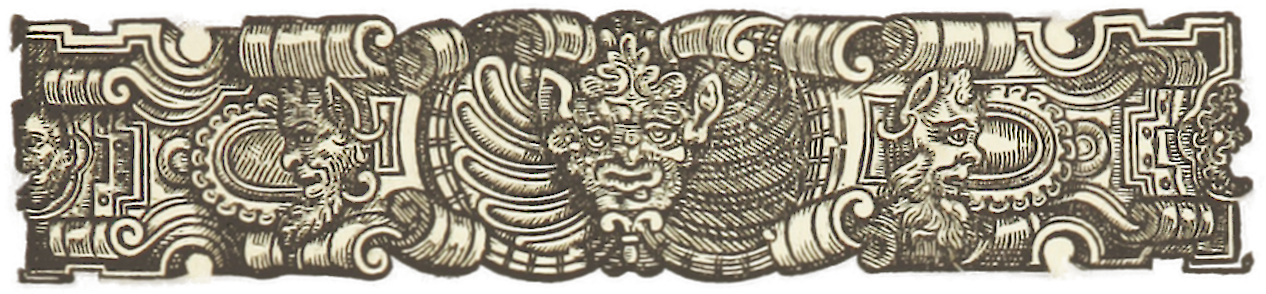
\includegraphics[width=\linewidth]{offene_lizenz/sailor_sepia}

Sollte die Gruppe sich nach dem Ascheregen oder ähnlich komplexen Themen erkundigen, werden sie an die Schamanin \textbf{Aschka} weitergeleitet.
Bezüglich des Qualmgeistes wird sie den Helden erklären, dass sie in ihrer Meditation ein Feuer in der Erde verspürt hat, das, als sie es näher betrachten wollte, ebenfalls angefangen hat, an ihrem Astralleib zu zehren.
Sie vermutet, dass die Hexen mehr wissen, zumindest wirkten diese bei Begegnungen zuletzt äußerst unstet.

\probe{beeinflussung}{Überreden (16)}{
Das Geheimnis des Weins wird sie den Helden nur mit einer gelungenen Probe verraten: Es ist nicht der Wein selbst, der das Jagdglück bringt, sondern die Karaffe, aus der er getrunken wird.
}
\probe{beeinflussung}{Überreden (20)}{Nur nach einer zweiten gelungenen Probe wird sie ihnen eine Karaffe übergeben.
Auf dieser liegt ein \biglittlecap{Adlerauge Luchsenohr}  (\ilaris{130}), der die Wahrnehmung der Jäger erhöht.
}


%\vfill
%
%\neuespalte

\absatz{Hexen im Rorwhed}
Im \textbf{Svelltal} gibt es mehrere \textbf{Hexenzirkel}. Der mächtigste davon ist der Zirkel im \textbf{Rorwhed}, der von der Oberhexe \textbf{Xerinn} angeführt wird.
Ein weiterer ist der des \textbf{Grauen Wald}es unter dem Oberhexer \textbf{Bringimox}.
Der \textbf{Graue Wald} hat den Hexen vom \textbf{Rorwhed} nach der Sprengung Asyl gewährt, was zu einer tiefen Freundschaft zwischen den Zirkeln geführt hat.
Die aufbrausende Katzenhexe \textbf{Xerinn} kämpft allerdings weiterhin mit der fulminanten Niederlage, die die Zerstörung des Tanzplatzes für ihre Pläne hinsichtlich der Macht im \textbf{Rorwhed} bedeutet.
Denn statt den Widerstand gegen die Orks weiterzuführen, muss sie nun sehen, wie sie Auflösung ihres eigenen Zirkels verhindert.

\begin{center}
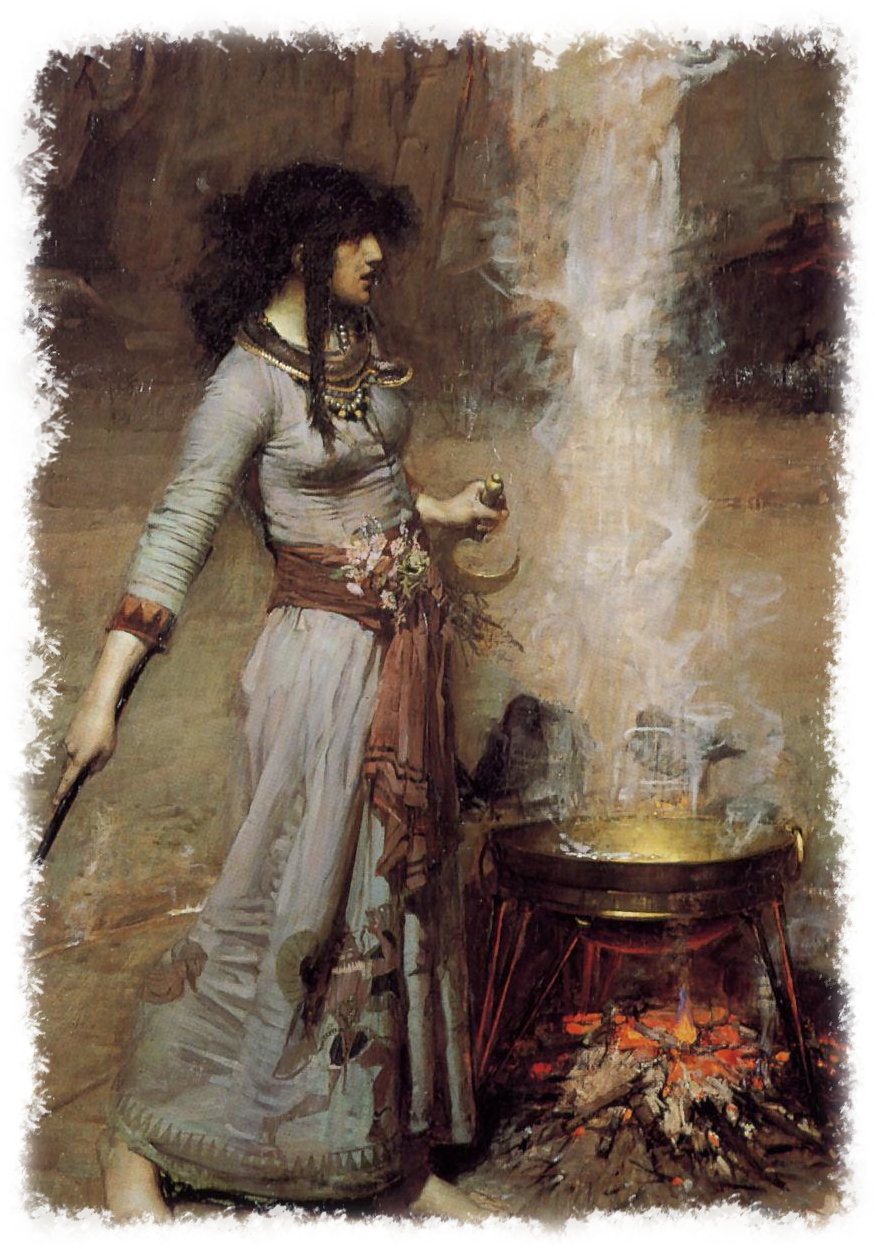
\includegraphics[width=0.91\linewidth]{offene_lizenz/hexe_distressed}
\end{center}
\columnbreak
Der Eulenhexer \textbf{Bringimox} sorgt sich dagegen mehr um das Loch in den Feenpfaden.
Als die beiden Anführer die Umgebung des Berges untersucht haben, haben sie den glühenden Dryadenbaum gefunden und konnten sich angesichts der Berichte über die brennenden Höfe und den Qualmgeist zusammenreimen, wie diese beiden Dinge zusammenhängen.
Sie sehen die Lösung in der Heilung des Baumes, wozu sie aber ausgewählte Leute aus beiden Zirkeln mit in das Tal der Dryade bringen müssen, die mit ihnen zusammen die Kraftfäden der Feenpfade wieder zusammenflicken und den magischen Brand in den Wurzeln des Baumes löschen.

Bisher sind sie noch nicht zur Tat geschritten, weil dieses Ritual zeitintensiv ist und sehr schmerzhaft für die Dryade sein wird.
Beide fürchten, dass der anhaltende Schmerz die Dryade zur Verwandlung zwingen wird, was ein lebensgefährliches Risiko für die Ritualteilnehmer darstellt.
Beide möchten aber auch, dass diese Angelegenheit von den Hexen selbst geregelt wird.

Sollten die Helden den Zirkeln von der inzwischen bereits aufgebrochenen Untersuchungseinheit der \textbf{Grauen Stäbe} berichten, werden sich die beiden Oberhexen zum Handeln gezwungen sehen.

\abschnitt{Finale im Tal der Dryade}
Die Hexen bereiten sich auf das Ritual vor, welches eine Stunde vor Mitternacht beginnen und die Kraftlinien und Feenpfade schließen soll.
Während sie es vollziehen, müssen sie durch die Heldengruppe geschützt werden vor den Angriffen des \textbf{Qualmgeist}es.
Falls es der Gruppe nicht schon klar ist, wissen \textbf{Bringimox} oder \textbf{Xerinn} zu berichten,
dass die \textbf{Dryade} des Tals identisch ist zu dem \textbf{Qualmgeist}, der des nachts umgeht.


Die Helden könnten auf die Idee kommen, mit der \textbf{Dryade} zu sprechen.
Sie hält sich tagsüber immer in ihrem Tal auf.
Es ist durchzogen von einem warmen, brenzligen Geruch.
Hier sind manche Büsche und Bäume noch grün und frisch, andere verkohlt, dazwischen stecken Felsbrocken, Überbleibsel der Detonation der Bergspitze.
Dazwischen steht einzeln der noch lebende, aber teils geschwärzte Baum der Dryade.
Vom Ritual rühren die langen Nägel, die in den Stamm eingeschlagen sind und ein großer, rot eingefärbter Stierschädel über einem Ast.

Wenn die Helden sich den Baum ansehen, erscheint sie:
Etwas größer als ein Mensch, so grün belaubt und schön wie es Dryaden eigen ist, aber auch müde und mit Ruß und Asche verschmiert.
Während des Gesprächs schließen sich verkohlte Stellen, doch anderswo stiebt erneut Asche auf.


Sie weiß um ihre Verwundung, aber erinnert sich nur verschwommen an die Nächte der letzten Wochen.
Auf jeden Fall macht sie den Helden klar, dass sie für nichts garantieren kann, sobald die Dunkelheit hereinbricht:
Ihre Qualmgestalt erscheint etwa zum Licht der ersten Sterne und dann hat sie keinerlei Kontrolle mehr.
Bis dahin können die Helden versuchen, den Hexen bei den Vorbereitungen zu helfen.


Sobald die Nacht hereinbricht, beginnt \textbf{Venaya} immer stärker zu qualmen.
Wie in vielen Nächten zuvor beginnt kurz danach eine Besessenheit, denn für die Geister ist sie in diesem Zustand ein offenstehendes Tor.
Wenn das geschieht, erhebt sie sich meist mit einem \biglittlecap{Leib des Windes} (\ilaris{147}\emph{f.}) in die Lüfte und lässt sich vom Wind weit ins Land tragen, um wahllos Gehöfte oder Reisende anzugreifen.

In Verteidigung gegen den Qualmgeist können die Helden auf einen schnellen Sieg im Kampf setzen.
Wenn sie besiegt wird, zerfällt sie zu Asche, unter welcher sie als Sprössling bis zum Morgengrauen neu heranwächst.

Oder sie können Magie einsetzen, um sie sich und den Hexen vom Leib zu halten:
\textit{Einfluss}zauber (\ilaris{133}) könnten sie auf Abstand halten, mit einem \biglittlecap{Harmoniesegen} (\ilaris{177}) wäre sie für eine Weile besänftigt, ein \biglittlecap{Geisterbann} (\ilaris{166}) könnte sie wieder in ihr natürliches Wesen zurückfinden lassen -- kreative Einfälle sollten belohnt werden.

\kreatur{Qualmgeist}{Ein Qualmgeist}{mythen}{
	\label{geist}
    \kreaturkampfwerte{8}{6}{5}{4}
    \trennlinie
    \kreaturvorteile{
        Aura (Hitze, Zähigkeit (20) alle 4 Initiativephasen, 1 Wunde), Flammenkörper (Alle Waffen, die Holz beinhalten, gelten gegen den Qualmgeist als Zerbrechlich (S. 47), Immunität (Feuer), Schmerzimmun I, Verwundbarkeit I (Wasser)}
    \trennlinie
    \kreaturwaffe{Feuerpranken}{1}{10}{16}{2W6+2}{Nachbrennen}
    \kreaturkampfvorteile{Zusätzliche Attacke I}
    \trennlinie
    \kreaturinfo{AsP}{64}
    \kreaturinfo{Feuer}{12 (Brenne toter Stoff!, Caldofrigo heiß und Kalt, Leib des Feuers, Wand aus Flammen, Warmes Blut, Zorn der Elemente)}
    \kreaturinfo{Luft}{10 (Aerofugo, Leib des Windes, Nebelwand und Morgendunst, Tlalucs Odem (Qualm statt Gestank))}
    \kreaturinfo{Eigenschaften}{8 (Atemnot)}
    \trennlinie
    \kreaturinfo{Beschreibung und Verhalten}{In ihrer nächtlichen Form ist die Dryade stark vom Vulkanismus gezeichnet, dessen Glut an den Wurzeln ihres Baumes nagt. Ihre feingliedrige Gestalt verkohlt und wird umhüllt von einer dichten Qualmwolke, die die Nacht noch mehr verdunkelt und auf Mensch und Tiere hustenreizend und erstickend wirken kann. Sie hat keinen Zugriff mehr auf das Element Humus, sondern wirkt Zauber aus den Bereichen Feuer und Luft, um Unbelebtes in Brand zu setzen und Lebewesen zu ersticken.}
}

Zum Kampfbeginn zaubert der Qualmgeist einen Nebelwand und Morgendunst (\ilaris{148}) in der Variation Geisternebel. Der Nebel hat durch den Schwelbrand ein rotes Glühen. Im Nebel tauchen als Verstärkung drei untote Wildschweine (\ilaris{108}) auf (sie zählen also nicht zur Kreaturenklasse "Tier" sondern zu "Untoter", \ilaris{99}). Sie sind aggressiv und greifen alles an, was sie als Eindringling sehen; also nicht die Dryade.

Das Ritual der Hexen dauert etwa zwei Stunden. Sobald dieses abgeschlossen wurde, hebt sich ein Windhauch durchs Tal, schüttelt kräftig die Baumkronen durch und die wilden Magieströme finden zu einer Ordnung zurück.
Die Verbindung der \textbf{Dryade} zu \textbf{Tairach}s Geisterwelt reißt ab und die Wunden im Tal können heilen.

\abschnitt{Der Mühen Lohn}

Nach Abschluss des Rituals bekommt jeder Held 30~EP.
Wenn die Gruppe ihre Verletzungen noch nicht selbst behandelt hat, werden sich die \textbf{Hexen} der beiden Zirkel darum kümmern.
Sie veranstalten außerdem eine schnelle Kollekte, bei welcher 20~Silber als Belohnung für die Gruppe herauskommen -- wenn die Helden noch Auftraggeber aus \textbf{Lowangen} mit ihrer Arbeit und ihren Ergebnissen zufriedenstellen konnten, lassen sich dort auch noch höhere Summen einstreichen. 

\begin{center}
\zeichnung[0.8\columnwidth]{gold.png}
\end{center}

Hexer \textbf{Bringimox} drückt einem der Helden noch etwas in die Hand:
Ein Vogelknochen, auf welchem ein Zauber liegt. Zerbricht man ihn, löst das einmalig einen \biglittlecap{Krähenruf} aus (\ilaris{134}).
Die \textbf{Dryade} kann zudem anbieten, von der Gruppe gesammelte Kräuter zu verzaubern, sodass sie lange frisch bleiben.

\neueseite

\abschnitt{Anhang}
\label{aiw_anhang}

\subsection[Pflanzen und Tiere]{Pflanzen}
Das Abenteuer spielt im Frühsommer, sodass sich viele örtlichen Pflanzenarten bereits zeigen und manche können auch schon geerntet werden. Entlang der Straßen und auf den Wiesen fallen darunter am häufigsten \textbf{Gulmond}, \textbf{Tarnele} und \textbf{Wirselkraut}, etwas seltener auch \textbf{Zwölfblatt}.

Am Waldrand hat man häufig Glück mit der \textbf{Vierblättrigen Einbeere}.

Nahe Flussufern und in Sümpfen wachsen \textbf{Donf}, \textbf{Roter Drachenschlund} und \textbf{Traschbart}.

\neuespalte

\subsection*{Tiere}
\label{svellt}
	Die Tierwelt im Svelltland ist typisch für Nordaventurien und besonders von der Nähe zum \textbf{Orkland} geprägt,
welches Tieren wie \textbf{Orklandhörnchen} und \textbf{-karnickel} den Namen gegeben hat.
Dabei bietet das Land ganz unterschiedliche Lebensräume:
In Wiesen und Auen leben \textbf{Rebhühner}, \textbf{Rehe}, \textbf{Rotpüschel}, \textbf{Pfeifhasen} und \textbf{Steppenhunde}.
Am Fluss gibt es \textbf{Fischotter}, \textbf{Biber} und \textbf{Molche}. All diese Tiere können die Helden zu Gesicht bekommen, ohne die Straße zu verlassen. In den weiten Ebenen leben sogar \textbf{Nashörner} und \textbf{Mammuts}.
Zu den Raubtieren zählen vor allem die \textbf{Silberwölfe}, die nicht nur im Rorwhed auftreten. Nur selten sieht man auch \textbf{Rauwölfe} und \textbf{Orklandbären.}

Erst abseits der Straßen im Wald findet man \textbf{Wildschweine}, \textbf{Streifendachse}, \textbf{Auerhühner}, \textbf{Waldwölfe} und (seltener) \textbf{Waldlöwen}. Dazu kommen in den Gebirgen auch \textbf{Böcke}, \textbf{Murmeltiere} und die \textbf{Halmar-Antilope}.

\spaltenende
\vfill
\begin{center}
\includegraphics[width=\linewidth]{offene_lizenz/svelt_distressed.png}
\end{center}


\neueseite
\spaltenanfang
\absatz{Kampfwerte}
\label{aiw_kampfwerte}

\kreatur{Bandit}{Bandit}{humanoid}{
	\kreaturkampfwerte{4}{5}{4}{2}
	\trennlinie
	\kreaturvorteile{Zweihändig}
	\trennlinie
	\kreaturwaffe{Keule}{1}{8}{8}{2W6}{Kopflastig, stumpf}
}

\kreatur{Riesenamöbe}{Riesenamöbe}{tier}{
	\kreaturkampfwerte{6}{14}{1}{2}
	\trennlinie
	\kreaturvorteile{Körperlosigkeit, Schmerzimmun II}
	\trennlinie
	\kreaturwaffe{Scheinarm}{1}{2}{6}{1W6}{Ätzend (Ein Opfer in der Umklammerung erleidet in jeder INI-Phase 2W6 SP), 	Umklammern (-2, die Riesenamöbe kann nur ein Opfer umklammern)}
}

\subsection[NSCs und generische Namen]{NSCs}
\unterabsatz{Lowangen}
\begin{itemize}
    \item \textbf{Kontor Stoerrebrandt}
        \begin{itemize}
        	\item  Valpo Lucianus von Sturzbach, Sekretär von Vanjescha Stoerrebrandt, blonde Haare mit gezwirbelten Schnauzbart, immer nach neuester horasischer Mode gekleidet, Zwicker in der Westentasche
        \item Palla und Lothar -- Angestellte des Kontors, freundlich, aber diskret
                \end{itemize}
    \item \textbf{Straßenbande}
                \begin{itemize}
        	\item  Leon Winkelhauser -- Veteran der Ork-Belagerung von 1031 BF, hat zwei Finger während einer Attacke verloren, grimmiges Auftreten
        \item Praiosmine Algerein -- hat ihren Verlobten während der Belagerung verloren, hübsches Gesicht
        \item Raul Zerte -- albernischer Söldner, ist nur aus Solidarität dabei
        \item Neowen Inveric -- war zu jung, um selbst in der Belagerung zu kämpfen, verehrt aber bis heute die \enquote{Helden} von damals
    \item Quin Lonnert -- ehemaliger Schmuggler, hat zwei Töchter, die Mutter ist kurz vor der Belagerung an einem Fieber gestorben
    \item Hierosebia Damicilia Pantalogereon, ehemalige fahrende Medica und Quacksalberin, heute Besitzerin einer kleinen Apotheke in Lowangen, weiches Herz für Außenseiter
    \end{itemize}
    \item \textbf{Ordenshaus Graue Stäbe}
                \begin{itemize}
        	\item  Barngrimm Radobrecht, den Großmeister des Ordens der Grauen Stäbe in Lowangen, kurze dunkle Haare und Bart, sanfte Stimme, tatkräftig, bodenständig, Vorurteile gegen Orks
      \item  Magistra ordinaria Vistella Jolen, hat den Ascheregen als magisch erkannt, strenges Gesicht, glatte blonde Haare, die nach hinten gekämmt sind
        \item Meera, Luis und Götz -- Adepten der Grauen Stäbe, tauschen sich über den neuesten Tratsch ihrer Vorgesetzen aus -- auch wenn sie ernsthafte Schwierigkeiten bekommen würden, wenn diese je erfahren würden, dass ihre Untergebenen die Verschwiegenheitsklausel nicht sonderlich ernst nehmen.
        \end{itemize}
        \end{itemize}
\vspace{-0.25cm}
\unterabsatz{Reise zum Rorwhed}
  \begin{itemize}
  	\item \textbf{Gasthaus}
                \begin{itemize}
        	\item  Der alte Strupp, sieht aus wie 90, arthritische Finger, kann aber noch gut erzählen
        \item Azzan (Ork), Gushrok (Ork), Kupunda, Gisbert und Koschrik -- begeisterte Zuhörer
        \end{itemize}
    \item \textbf{Niedergebranntes Gehöft}
                \begin{itemize}
        	\item Bauernpaar Arba und Bredo Wollweber
        	\end{itemize}
\end{itemize}
\vspace{-0.25cm}
\unterabsatz{Rorwhed}
     \begin{itemize}
   	\item \textbf{Hexenzirkel}
                \begin{itemize}
        	\item  Xerinn, eigeborene Schöne der Nacht, Oberhexe des Rorwhed-Zirkels, aufbrausend und kontrollierend, wallende rote Haare und katzengrüne Augen
       \item Bringimox, Mitglied der Verschwiegenen Schwesternschaft, Oberhexer des Grauen Waldes, berechnend, aber sanftmütig, weiße Haare, haselnussbraune Augen, überraschend muskulös für sein Alter
        \item Alvina, Schlangenhexe, dunkle Haare, tiefblaue Augen
        \end{itemize}
    \item \textbf{Goblins}
                \begin{itemize}
        	\item  Schamanin Aschka, die Verhüllte, ältere Goblinfrau, geduldig, aber vorsichtig, Vorurteil gegen bunt gekleidete Figuren
        \item Jägertrupp: Wassel, Broggo, Juulka und Frikka -- aufgeregte Jäger, die von der Schamanin den Auftrag erhalten haben, die Wildschweinfässer zu fangen
        \end{itemize}
    \item \textbf{Menschlich-orkische Jägergruppen}
            \begin{itemize}
    	\item Herdlind Silkwies -- wettergegerbte Jägerin, silberne Haare
        \item Avon Mühlenfels -- Spezialist für Wildschweinjagd, dicker Pelzmantel
        \item Sequin Winterkalt -- junger Rotschopf, trägt einen Fuchsschädel als Glücksbringer am Gürtel
        \item Korobai Felsvater, stoischer älterer Burrkuzk-Ork, guter Fallensteller
        \item Grashok Drachenschelle, reizbarer Burrkuzk-Ork, soll einen Drachen geohrfeigt haben
        \end{itemize}
    \item \textbf{Dryade Venaya}, etwas größer als ein Mensch, grün belaubt, schön, müde und mit Ruß und Asche verschmiert
    \end{itemize}

\info{
    \subsection*{Generische Namen}
    \textbf{weiblich:}
    Dramina Gesse, Glenna Fassmacherin, Ilke Gerrholt, Traute Netzknüpferin
    
    \textbf{männlich:}
    Drego Rastburger, Elfwyn Kevendoch, Irian Dinckel, Gerding Linnenschneider
}

\spaltenende



\chapter*{In den Hallen\linebreak des Bergkönigs}
\addcontentsline{toc}{chapter}{In den Hallen\allowbreak\ des Bergkönigs}

\thispagestyle{empty}

\begin{center}
\zeichnung[0.69\textwidth]{cover-bergkoenig.png}\\
\usekomafont{section}Matthias Ott\normalfont\normalcolor\normalsize
\end{center}

\credit{Illustrationen}{\href{https://www.artstation.com/bernhard\_eisner}Alnus (Anton Dobsak)\\
	{Bernhard Eisner}\\
	\href{https://www.zillie-zeh.de/}{Zillie Zeh}\\	
	game-icons.net
}
\credit{Mit Dank an}{Kilian Linder für konstruktives Feedback,\\ Xaver Stiensmeier für die Ausrichtung des Wettbewerbs und Odir Sensendengler\\ sowie die geduldige Testgruppe: Jascha, Gloria, Meike und Hannes
}

\newpage

\platz

\credit{Autor}{Matthias Ott}

\credit{Illustrationen}{\href{https://www.artstation.com/bernhard\_eisner}{Bernhard Eisner}\\game-icons.net
}
\credit{\LaTeX-Klasse}{Lukas Ruhe}

\credit{Mit Dank an}{Kilian Linder für konstruktives Feedback,\\ Xaver Stiensmeier für die Ausrichtung des Wettbewerbs und Odir Sensendengler\\ sowie die geduldige Testgruppe: Jascha, Gloria, Meike und Hannes
}

\newpage
\spaltenanfang


\addcontentsline{toc}{section}{Einleitung\,für\,die\allowbreak\ Spielleitung}
\section*{Einleitung für die Spielleitung}
In diesem Abenteuer kann eine Gruppe in \textbf{Finsterkoppen},
der Hauptstadt des Bergkönigreichs eines zwergischen Volkes im \textbf{Finsterkamm},
eine Intrige um die Einsetzung eines Hochkönigs aufdecken und damit die Spaltung in zwei Völker auslösen.

Dies ist auch der Plot von \emph{Im Traumlabyrinth} (Schmidt Spiele, 1990).
Während die Ergebnisse dieses Abenteuers in jüngeren Publikationen (wie \emph{Angroschs Kinder} (Fanpro, 2005))
übernommen wurde, passen die Inhalte des Abenteuers selbst nicht in das später entwickelte Aven\-turien\-bild und ergeben auch keinen spannenden Spielabend.
Ich wollte daher die Möglichkeit bieten, die historische Entwicklung im Rahmen einer anderen Handlung miterleben zu können
und dabei Orte und Figuren kennen zu lernen, die in später stattfindenden Abenteuern wieder eine Rolle spielen (können).

Den Schauplatz \textbf{Finsterkoppen} und die \textbf{Finsterkopp-Binge} waren schon im Computerspiel \emph{Sternenschweif} (Attic, 1994) zu erkunden. %, das ich vor etwa 20 Jahren das letzte Mal gespielt habe.
%Was mir davon noch in Erinnerung war, habe ich verarbeitet.
Ich habe für den Anhang auf die Liste der Gebäude aus \link{https://www.kunar.eu/nlt/finsterkoppen.htm}{Kunars Reiseführer} zurückgegriffen.
Die Idee von Rattengold als überschwerem 13.\,Unmetall haben Simon Schollenberger, Stefan Weber und Stefan Löffler für das Wettbewerbs-Abenteuer \enquote{\link{https://www.orkenspalter.de/filebase/index.php?file/53-totgeboren/}{Totgeboren}} entwickelt.
Auch wenn sie den Weg ins kanonische Aventurien noch nicht gefunden hat, habe ich sie hier aufgegriffen.


\subsection*{Aufbau und Verlauf}
Ich habe das Abenteuer in drei Akte unterteilt, die nach meiner Einschätzung jeweils eine bis zwei Stunden Spielzeit ergeben sollten.
Sie bauen inhaltlich aufeinander auf.
Neben den beschriebenen Schlüsselszenen kann Ihre Gruppe durch eigene Schwerpunktsetzungen die Handlung mitbestimmen -- beispielsweise,
indem sie im \emph{ersten Akt} mit der Bevölkerung von \textbf{Finsterkoppen} Handel treibt oder im \emph{zweiten Akt} weitere Räumlichkeiten erkundet.
Wegen des beschränkten Platzes müssten Sie die dazugehörigen Szenen jedoch gemeinsam improvisieren.

Zu Ihrer Orientierung ist zu Beginn jedes Aktes angegeben, welche Ziele die Gruppe hier verfolgen (und gegebenenfalls erreichen) sollte.
Ebenso gebe ich hier Tipps, wie Sie -- falls die Zeitplanung für Sie nicht passt  oder der Abschnitt Ihrer Gruppe keinen Spaß machen würde -- ein längeres oder kürzeres Spiel erreichen könnten.

Im \emph{ersten Akt} wird die Gruppe an das Problem herangeführt:
Die Gruppe bringt die Nachricht einer äußeren Gefahr in die Stadt.
Um dieser zu begegnen, würde der \textbf{Tiefe Rat} der Finsterkamm-Zwerge gern einen Hochkönig wählen.
Der greise Bergkönig \textbf{Gerambolosch}, der das Verfahren einleiten muss (und der natürliche Kandidat für dieses Amt wäre), ist jedoch nicht ansprechbar -- wie es scheint, aus Altersgründen.
Die einzige Alternative ist, das \textbf{Szepter der Stärke} durch den örtlichen Hochgeweihten des Angrosch neu schmieden zu lassen.
Das Szepter lagert jedoch in einer alten Binge, die die Finsterkamm-Zwerge nicht mehr betreten wollen.

\kasten{\enquote{Binge} ist ein Fantasie-Wort, das zwergische unterirdische Anlagen  beschreibt, die sowohl Bergwerk als auch Wohnsiedlung umfassen.}

Die Suche führt die Gruppe im \emph{zweiten Akt} in ebendiese Hallen.
Hier gilt es, Fallen zu entgehen, Wühlschrate zu ertragen und schließlich ein Rätsel zu entschlüsseln, um Zugang zum Szepter zu erhalten.
Eine Begegnung mit einem \textbf{Bosnickel} gibt den Hinweis, dass das Unmetall \textbf{Rattengold} in der Binge zu finden ist.
Die Gruppe entdeckt, dass jemand davon an die Oberfläche bringt.
\kasten{\enquote{Unmetalle} sind Materialien, die in der Regel Dämonen zugeordnet werden. Einzige Ausnahme ist das hier vorkommende, dem Namenlosen zugeordnete \textbf{Rattengold}. Ihre Eigenschaften sind nicht festgelegt.}

Im \emph{dritten Akt} versucht die Gruppe herauszufinden, wer dies gewesen sein könnte.
So kann es ihnen gelingen, während der Hochkönigwahl den Intriganten \textbf{Bonderik} zu enttarnen,
der diese zu seinen Gunsten beeinflussen wollte.

\subsection*{Was wird zum Spielen benötigt?}
Für erfahrene Spielleitungen dürfte das Abenteuer selbst sowie die Ilaris-Regeln als Grundlage zur Gestaltung des Spielabends ausreichen.
Wenn Sie mit der Welt Aventurien noch nicht viel Kontakt hatten, empfehle ich zur Vorbereitung den Band \emph{Angroschs Kinder} (Fanpro, 2005, im folgenden \emph{AK}).
Dieser Band ist leider vergriffen und gebraucht kaum erhältlich.
Günstiger ist \emph{Die Zwerge Aventuriens} (Schmidt Spiele, 1993, im folgenden \emph{DZA}) gebraucht zu bekommen,
das jedoch älter und weniger umfangreich ist.

Ebenso empfehle ich weniger erfahrenen Spielleitungen einen Blick in eine Spielhilfe zum Thema Dungeon.
\emph{Katakomben und Kavernen} (Ulisses, 2010, im folgenden \emph{KK})
ist noch als ebook erhältlich.
Die kostenfreie Spielhilfe \enquote{\link{https://www.orkenspalter.de/filebase/index.php?file/2724-fackelschein-und-kellerstaub/}{Fackelschein und Kellerstaub}} von Ulrich Lang
zum selben Thema ist meines Erachtens ähnlich nützlich.

Ich habe darauf verzichtet, eine Karte der Finsterkopp-Binge anzufertigen, weil die genaue Platzierung der beschriebenen Räume zueinander keine Rolle spielt und ich mir die Freiheit erhalten wollte, sie nach dramaturgischen Gesichtspunkten spontan umzuverteilen. Wenn Ihre Gruppe großen Spaß an Karten hat oder Sie mehr Anregungen für die Ausgestaltung der Details suchen,
finden Sie in \textbf{Malatosch} (\emph{KK:147}) ein geeignetes Vorbild für zwergische Architektur.

\subsection*{In eine andere Zeit verlegen?}
Unsere Testspiel-Gruppe hat die Dringlichkeit einer Hochkönigwahl selbst hergestellt, indem sie die Botschaft von einer drohenden Orkgefahr nach Finsterkoppen brachte.
Mit dieser Prämisse lässt sich das Abenteuer problemlos im Zeitraum vom Auftauchen Ashims 1003 bis zum Einfall der Orken ins Svellttal 1010\,BF verschieben
und etwa mit der Suche nach dem  \textbf{Salamanderstein} (vgl. \emph{Sternenschweif}) verbinden.

Wenn Sie näher an der aventurischen Jetztzeit spielen, sich jedoch eng am aventurischen Kanon orientieren, sitzt der Hochkönig des \fkvs fest im Sattel,
während sein Konkurrent sich als Anführer der \textbf{Finsterzwerge} in der südlichen Hälfte des \textbf{Finsterkamm}-Gebirges eingerichtet hat.
Nach dem dritten Orkensturm sollten Sie die Ereignisse also in einer anderen Zwergenstadt spielen lassen und die Namen der Nichtspielerfiguren austauschen.

Die äußere Gefahr, die Anlass der Hochkönigwahl wird -- bei mir ein Orkangriff --, tritt im Abenteuer noch nicht ein. Sie können sie für Ihre Gruppe frei festlegen.
Ein Drache, eine Naturkatastrophe oder eine in der Nachbarschaft grassierende Seuche wären beispielsweise andere Möglichkeiten, die die Zwerge bewegen können, einen Hochkönig zu wählen.

\subsection*{Welche Gruppen sind geeignet?}
Das Abenteuer ist für eine Gruppe von rund 4.000 Erfahrungspunkte nach dem Ilaris-System ausgelegt. Vorgefertigte Beispiel-Figuren finden Sie im Anhang.
Vorausgesetzt werden \textbf{Rogolan}-Kenntnisse bei mindestens einem Gruppenmitglied sowie ein gewisses Interesse an zwergischer Kultur und dem Wohlergehen des Bergkönigreichs.
Orks und Echsenmenschen sind sicher ungeeignet, weil das \fkv ihresgleichen nicht in ihrer Stadt dulden würden.
Goblins und (Halb-)Elfen werden mit Anfeindungen und Unverständnis zu kämpfen haben.

Grundsätzlich spricht nichts dagegen, das Abenteuer auch mit einer rein zwergischen Gruppe zu spielen.
In diesem Fall liegt eine Herausforderung darin,  das Besondere an zwergischer Kultur für ihre Mitspielenden rüberzubringen,
während es für ihre Figuren selbstverständlich ist.
Sie können jedoch davon ausgehen, dass das \fkv ein durchaus eigenes Völkchen ist.
Viele Details dürften daher auch für  Vettern und Cousinen aus dem Eisenwald oder Amboss-Gebirge erwähnenswert sein.

\subsection*{Themen, Motive und Verbindungen}
Das Abenteuer ist kompakt, ermöglicht  ihrer Gruppe jedoch den Einstieg in eine zwergische Kultur
-- im wahrsten Sinne des Wortes, geht es doch hinab in Abschnitte einer Binge,
die das \fkv selbst nur noch in  Ausnahmefällen betritt.

Legen sie daher Wert darauf, diese Kultur auch vorzustellen. Das Abenteuer bedient hier insbesondere
\begin{itemize}
	\item das andere Zeitgefühl der langlebigen Spezies,
	\item die Bindung an die Tradition und Misstrauen gegenüber anderen Völkern,
	\item der hohe Respekt vor dem Alter und
	\item die an Sturheit grenzende Konsequenz.
\end{itemize}

Sie können hier  Spuren zur untergegangenen \textbf{Binge Umrazim} (\emph{KK:173}) legen,
falls ihre Gruppe im späteren Spiel nach diesem großen Geheimnis der Kinder Angroschs suchen soll.
In diesem Sinne habe ich es an \emph{Wohin der Schatten fällt} von Kathrin Lieb (in: \emph{Ehrenhändel} (FanPro, 2006)) angeschlossen,
wo ebenfalls Hinweise auf \textbf{Umrazim} zu finden sind.

Ebenso ruht unter \textbf{Finsterkoppen} -- tiefer, als dieses Abenteuer führt -- bis 1011 BF der \textbf{Salamanderstein}, der als Zeichen des \textbf{Saljeth-Paktes} Symbol des geeinten Kampfs von Kindern Angroschs und Elfen gegen die Orkgefahr darstellt.
Die Suche nach diesem Artefakt könnte die Gruppe nach \textbf{Finsterkoppen} führen.
Genauso wäre es möglich, einige Jahre später im Rahmen dieser Suche zurückzukehren.
Und hat der Salamanderstein nicht vielleicht etwas mit dem \textbf{Stein der Simia} (\emph{Brogars Blut}, Fanpro 1998), dem \textbf{Feuer Ingras} (\emph{Feuerbringer}, Ulisses 2013) oder \textbf{Angrosch ka Broschrardosch} (\emph{KK:111}) zu tun?

Weitere verlassene Bauten der Finsterkamm-Zwerge kommen in den Abenteuern \emph{Odem der Kälte} (Fanpro, 2010) sowie \emph{Das Geheimnis des Drachenritters} (Ulisses, 2019) vor.
\spaltenende
\begin{center}
	\zeichnung[0.75\textwidth]{Drache.jpg}
	\end{center}

\neueseite

\section{Erster\,Akt: Der Tiefe Rat}
\spaltenanfang
\info{\textbf{Ziel der Gruppe:} Das \fkv über die Gefahr informieren und den Auftrag erhalten, das Szepter zu suchen.

\smallskip

	\textbf{Vorschläge für längeres Spiel:}
	\begin{enumerate}
		\item Finsterkoppen im unwegsamen Finsterkamm zu finden kann ein Abenteuer für sich sein.
		Mehr dazu \link{https://brauerei.ilaris-online.de/share/jD-nmdtQr4ZM}{hier} (work in progress).
\item Nehmen Sie sich Zeit, Finsterkoppen zu erkunden -- nutzen Sie die Ortsbeschreibung im Anhang. Der \textbf{Tiefe Rat} kommt erst in einigen Tagen zusammen, zuvor kann die Gruppe gemeinsam ein zünftiges Pilzbier bei \textbf{Schwarzbart} trinken,
	von \textbf{Muragolosch} auf offener Straße ausgeschimpft werden,
	bei \textbf{Gandrasch} eine besondere Armbrust zu bestellen versuchen oder \textbf{Turgol} nach Geheimnissen der Geoden fragen --
	Bitten, die jetzt vielleicht abgeschlagen und nach dem dritten Akt erfüllt werden.
		\end{enumerate}
	\smallskip
	\textbf{Vorschläge für kürzeres Spiel:}
		\begin{enumerate}
		\item Lassen Sie die Gruppe statt der in der Ratsversammlung auf S.\,\pageref{idee} vorgesehenen Recherche noch in der Ratsversammlung eine \emph{Gebräuche-Probe (Zwerge, 24)} würfeln.
		Misslingt sie, geschieht nichts schlimmes, sondern \textbf{Bonderik} bringt das Wissen um das Szepter ein und wird von Inradon \textbf{Xermosch} bestätigt.
	\item	Auf dem \textbf{N\^orrnstieg} wird die Gruppe von einer zwergischen Schar mit vorgehaltenen Armbrüsten überfallen.
	Sie sollen eine Schatz -- das Szepter -- aus einer Binge bergen, die das \fkv selbst nicht mehr betreten will.
\end{enumerate}
}

\subsection{Finsterkoppen}
Finsterkoppen ist die Hauptstadt des Finsterkamm-Volkes.
Der Begriff \enquote{Stadt} trifft es nicht ganz: zumindest unterirdisch hat Finsterkoppen keine klare Grenze.
Die Wohnhöhlen, Minen und Bingen ziehen sich weit unter dem Gebirge hindurch.
Jede Sippe dürfte ein anderes Verständnis dafür haben, was davon noch zu Finsterkoppen gehört.

Vier Besonderheiten kommen jedoch auf engem Raum zusammen und machen deutlich, dass hier das politische und geistliche Zentrum des Bergkönigreichs liegt:
\begin{itemize}
	\item ein teilweise aufgegebenes und verschlossenes Bergwerk, das den Aufzeichnungen zufolge der Ausgangspunkt der zwergischen Besiedelung des Finsterkamms war (es wird im \emph{zweiten Akt} näher erkundet)
	\item der damit verbundene, zentrale \textbf{Angrosch}-Tempel (s. S.\,\pageref{angrosch})
	\item die Versammlungshalle/Halle des \textbf{Tiefen Rats} (s.\,u.)
	\item (für eine zwergische Siedlung)  ungewöhnlich viele oberirdische Gebäude, die auch den endgültigen Sieg über Horndrachen und Orks verdeutlichen,
	die in anderen Ecken des Gebirges durchaus noch Gefahren darstellen.
\end{itemize}

In diesem Abschnitt sind nur die zwei Schauplätze beschrieben, an denen die Handlung spielt: Die Versammlungshalle (in der der \textbf{Tiefe Rat} tagt) und der Angrosch-Tempel (durch den die Gruppe die Binge betreten kann). Weitere Details zu Finsterkoppen als Abenteuerschauplatz finden Sie im Anhang mitgeliefert.

\kasten{Großlinge würden vielleicht von einem \emph{Hohen Rat} sprechen -- deutliches Zeichen, dass die Sonne ihnen das Haupt verbrannt hat.
	Selbstverständlich ist es der \textbf{\emph{Tiefe} Rat}, was die \emph{tiefe} Weisheit seiner Mitglieder und Bedeutung seiner Beschlüsse anzeigt!}

\vfill

\subsubsection{Die Versammlungshalle}

\vorlesen{\label{halle}
Die Versammlungshalle verbindet das große Tor mit dem Angroschtempel. Vier weitere Gänge führen seitlich tiefer in den Berg.
Die Halle ist für zwergische Bedürfnisse wahrlich großzügig bemessen -- bei wichtigen religiösen Zeremonien finden mehrere Tausend hier Platz.
Im Verteidigungsfall können große Geschütze aufgestellt und auf den Gang gerichtet werden.
Häufiger dient sie zu repräsentativen Zwecken wie dem Empfang hohen Besuchs anderer Völker -- und den regelmäßigen Sitzungen des \textbf{Tiefen Rat}s.\\
In zwei Reihen sind je vier Podeste angeordnet, ein neuntes -- das des \textbf{Bergkönig}s -- an ihrer Stirnseite.
}

Die Podeste haben auch außerhalb der Ratssitzungen ihren Sinn.
Hitze aus dem Schlot des Berges wird nämlich durch ein sinnreiches Röhrensystem auch unter den Boden der Halle geleitet.
In etwa ein Spann großen Öffnungen auf den Podesten findet dieses System Ausgang, so dass sich einerseits kein Überdruck aufbaut,
wenn \enquote{Väterchen Angrosch mal kräftiger heizt} und andererseits solche spontanen Entladungen  nicht entlang von Laufwegen auftreten.

Regelmäßig flimmert daher die Luft über den Podesten vor Hitze, seltener treten schweflig riechende Wolken aus,
noch seltener Gase, die Traumbilder verursachen. Erst bei einer Hand voll Gelegenheiten in tausendjährigen Geschichte dieser Halle ist so ein Austritt mit einer Ratssitzung zusammengefallen;
das \fkv interpretiert diesen Einfluss auf die Ratsmitglieder als direkte Inspiration durch Angrosch.

\subsubsection{Der Angroschtempel}\label{angrosch}
\vorlesen{%
Im gesamten Tempel ist es \emph{heiß} \emph{(Ilaris:35)}, da stets mehrere Feuer und Öfen brennen.
Seine Grundfläche entspricht etwa der der Versammlungshalle, doch gibt es hier mehr Nischen mit \textbf{Altäre}n -- oft zugleich Werkbänke oder Ambosse.
Die Wände sind mit Angram-Runen bedeckt, die die Geschichte der Kinder Angroschs im Allgemeinen und des \fkv im Besonderen im Lichte des Angrosch-Glaubens auslegen.\\
Den Platz der heiligen Flamme nimmt in diesem Tempel ein sechs Spann breiter \textbf{Schlot} ein, der direkt senkrecht in das vulkanische Herz der Berge führt.
Hier hinein werden Opfergaben und die Toten aus dem \fkv geworfen.
Die Hitze aus der Tiefe ist in zwei Schritt Umkreis deutlich spürbar (\emph{Kh\^omglut}, \emph{Ilaris:35}).
Hier treten mehrmals pro Jahr  und in höherer Konzentration als in der Versammlungshalle Gase aus, die bei empfindlichen Zwergen und Menschen Atemnot,
bei empfänglichen (\emph{Vorteil: Prophezeien (Ilaris:30)} zudem Visionen auslösen können.
\\
Hinter dem Schlot führen einige Stufen hinauf zum großen Altar-Amboss. Auf dessen Rückseite setzen sich die Stufen zu einer langen \textbf{Treppe} hinab in die Dunkelheit fort.
}

Diese Treppe endet vor einer kleinen Halle, die außer einigen alten Kohlebecken nichts enthält.
Ein stets verschlossenes \textbf{goldenes Portal} führt von hier aus in den aufgegebenen Teil der Finsterkopp-Binge.

\zeichnung[0.3\textwidth]{hammer.png}

\subsection{Zur Ratsversammlung}
\subsubsection{Der Tiefe Rat}
Der \textbf{Tiefe Rat} trifft jene Entscheidungen, die das  gesamte Bergkönigreich angehen.
Er setzt sich aus den Häuptern der acht bedeutendsten Sippen zusammen.
Mit dieser Zahl erinnert das traditionsbewusste \fkv an die acht Stammväter und acht Stammütter (\emph{AK:8}) --
seit Beginn der Siedlung sind somit immer acht Sippen vertreten gewesen, auch wenn sich alle paar Jahrhunderte ändert, welche acht.


Diese acht wählen aus ihrer Mitte den \textbf{Bergkönig} oder die \textbf{Bergkönigin}, für die dann ein weiteres Mitglied aus derselben Sippe nachrückt.
Als Anführer der Golgrasch-Sippe tritt an Stelle von Bergkönig \textbf{Gerambalosch Sohn des Gengram} somit dessen Sohn
\textbf{Garbalon} (tatkräftig, schlägt darum gern die Hände zusammen) auf.

\neuespalte

Die übrigen Sippen sind vertreten wie folgt:
\begin{itemize}
	\label{rat}
\item \textbf{Bonderik} (schwarzhaariger Zwerg mit knarzender Stimme, legt die Fingerspitzen aneinander)
\item \textbf{Parsezel Sohn des Pemoin} (Zwerg, spricht aufgeregt, wirft an passenden und unpassenden Stellen ein \enquote{oder?} ein)
\item \textbf{Rodrik} (ungewöhnlich dicker Zwerg, der gern in ein- und zwei-Wort-Sätzen spricht, klopft sich aufs Knie, wenn er fertig ist)
\item \textbf{Barselok} (weißhaarige Zwergin, die jeden Satz mit einem gesummten mmmh beginnt)
\item \textbf{Fendor} (außerordentlich gutaussehender Zwerg, unterstreicht seine Worte mit Fingerspiel)
\item \textbf{Drumbal} (Zwerg, der beim Sprechen kaum die Zähne auseinander nimmt)
\item \textbf{Borsok}  (von vielen Kämpfen vernarbte Zwergin)
\end{itemize}

Der Geode \textbf{Turgol} (Kapuze stets tief ins Gesicht gezogen, denkt über jedes Wort dreimal nach) ist von der Hand voll \textbf{Geoden}, die es im Finsterkamm gibt, als ihr Sprecher anerkannt.
Am Rat nimmt er jedoch als Berater des Bergkönigs teil und hat selbst keine Stimme.

Der Hochgeweihte (\enquote{Inradon}) \textbf{Xermosch} des örtlichen Angrosch-Tempels 
(kahlköpfig, bezieht sich in jedem zweiten Satz auf Angrosch) ist offiziell ebenfalls nur beratend bei den Sitzungen des tiefen Rates.
Im Gegensatz zu den abergläubisch gefürchteten Geoden kann er aber voraussetzen, dass seinen Worten Gewicht beigemessen wird.

\info{Vermutlich wird es für Ihre Gruppe -- und für Sie -- zu unübersichtlich, wenn sie in der Versammlung alle Ratsmitglieder inklusive den beiden Beratern als Sprechrollen führen. Nutzen Sie \textbf{Bonderik} als klugen Mahner, \textbf{Garbalon} als sympathischen Aktionisten,  \textbf{Borsok}, um der Gruppe kontra zu geben und \textbf{Xermosch} als Wissenshüter.\\Dennoch ist es nicht schlecht, weitere Rollen in der Hinterhand zu haben, falls auch in Ihrer Gruppe unterschiedliche Positionen eröffnet werden und die Verhandlungen sich im Spiel in die Länge ziehen.}

\kasten{\textbf{Bergkönig oder Hochkönig?}
	
	Das ständige Amt, das die Menschen als \enquote{\textbf{Bergkönig}} bezeichnen, ist nicht mit den  Befugnissen ausgestattet, die man gemeinhin für einen König erwartet.
	Es handelt sich eher um einen obersten Friedensrichter des jeweiligen zwergischen Volkes.
	Gerade im \fkv\ ist seine formale Macht begrenzt -- er ist lediglich Vorsitzender des Tiefen Rates ohne eigenes Stimmrecht.
	Nur bei Stimmengleichstand obliegt es ihm, den Ausschlag zu geben.
	
	In Zeiten äußerer Gefahr oder großer Not wählen die Zwerge dagegen \textbf{Hochkönig}e --
	formal über alle Kinder Angroschs, wobei gerade das \fkv\ sich schon öfter nicht die Mühe gemacht hat,
	andere Völker in die Wahl einzubeziehen oder die Anerkennung des Hochkönigs von diesen zu verlangen.
	
	Vom Hochkönig wird gemeinhin erwartet, dass er sein Amt aufgibt, wenn die Gefahr vorüber ist.
}

\subsubsection{Der Ablauf der Sitzung}

\textbf{Auftritt des Bergkönigs}

\label{ratssitzung}
\vorlesen{%
Der Bergkönig wird von vier kräftigen Angehörigen seiner Sippe auf einem Stuhl mit hoher und reich verzierter Lehne hereingetragen.
Sie setzen ihre Last ab, ziehen die Tragestangen heraus und ziehen sich unauffällig zurück.

\textbf{Gerambolosch}s mit Hermelinfell gesäumte Robe aus schwerem roten Samt wallt über dem Kettenhemd, das mit breiten goldenen Armreifen am Handgelenk
 abschließt.
Der prächtige weiße Bart ruckt auf der Brust des Bergkönigs hin und her,
 den Bewegungen seines herabgesunkenen Kopfs folgend, wie man es von Schlafenden kennt. Die Lider sind halb über die Augen gesunken. Deren untere Hälfte wirkt milchig.
\\
Nachdem der Stuhl abgesetzt wurde, lässt \textbf{Gerambolosch} keine Regung mehr erkennen.
}


\textbf{Der Bericht}

	Statt dessen ergreift \textbf{Xermosch} das Wort (selbstverständlich auf Rogolan):

\label{gefahr}

\vorlesen{%

	
\enquote{%
	Geschätzter König Gerambolosch, hochverehrte Mütterchen und Väterchen: Angrosch ist mein Zeuge, viele Fragen treiben den Tiefen Rat heute um.
Tauwetter steht uns bevor und wie jedes Jahr müsst Ihr beschließen, wann welche Schleuse geöffnet und welche Weide bewässert werden soll.
Angroschs Tempel in Hilltorp erbittet einen weiteren Baumeister für die Reparatur eines Amboss-Sockels in der Tempelhalle.
	
	Zu allererst würde ich jedoch gern einen Punkt aus der Welt außerhalb unseres von Angroschs gesegneten Bergkönigreichs aufrufen:
	Die Fremden, die Ihr hier vor euch seht, berichten von einer -- weiß Angrosch! -- großen Gefahr.
	Wir haben sie darum gebeten, persönlich vor Euch zu erscheinen, damit Ihr den Bericht aus ihrem eigenen Munde hört.
	So keine Gegenrede besteht, wollten wir ihnen unter Angroschs Augen das Wort erteilen.}
}

\textbf{Bonderik} erhebt eben solche:

\vorlesen{%
\enquote{Hochverehrter Vater Xermosch, Eile mit Weile und alles, wie es Angrosch gefügt! Wie Ihr selbst sagt, sind es Fremde.
Einige von ihnen nicht einmal Angroschim. Ich würde doch gern zunächst wissen, um wen es sich handelt und ob es vertrauenswürdige Leute von Stand und Ansehen sind, bevor ich ihnen mein Ohr leihe.}
}

\info{Die Gruppe hat nun Gelegenheit, von ihrer Person und ihren bisherigen Taten zu berichten.
Menschlicher Adel und akademische Erfolge -- selbst ein Krieger*innenbrief -- zählen wenig.
Siegreiche (oder doch zumindest mutige) Kämpfe gegen Drachen, Oger und Orks wissen die Ratsmitglieder dagegen zu schätzen.}

\info{%
Legen Sie die Latte für Vertrauenswürdigkeit nicht zu hoch. Der anschließende Konflikt soll sich am Umgang mit der Gefahr entzünden, nicht die Wahrheit des Berichts in Zweifel gezogen werden. Anschließend werden sie daher gebeten, die drohende Gefahr darzustellen. %Nutzen Sie die Möglichkeit, durch gelegentliche kurze Einwürfe die übrigen Ratsmitglieder vorzustellen.
In der Diskussion sollte deutlich werden, dass das \fkv gewohnt ist, sich gegen alle Gefahren in den Stollen und Höhlen seines Bergkönigreichs zu verschanzen.
Verantwortung für die Reiche der Menschen oder gar Elfen übernimmt es nicht.
}

Während des Berichts zeigt der Bergkönig weiterhin kein Zeichen des Zuhörens oder des Erwachens. Wer bewusst darauf achtet, kann immerhin ab und an Heben und Senken der Brust erkennen.
Der Bergkönig lebt.

\probenkasten[
bild=wahrnehmung,
zusammenarbeit=nein,
gruppenprobe=nein,
pw=12,
farbe=gruen,
erfolg={},
misserfolg={}
]{Menschenkenntnis}{%
 Die übrigen Teilnehmenden scheinen \textbf{Gerambolosch}s Zustand vollständig zu ignorieren. \\
 \textbf{16:} Sie unternehmen sogar bewusste Anstrengung, ihn nicht anzusprechen oder direkt anzusehen.\\
 \textbf{20:} Der Zustand scheint ihnen unangenehm oder peinlich zu sein.\\
 \textbf{24:} Offensichtlich befürchten die Teilnehmenden, dass \textbf{Gerambolosch} in den Zustand der Vergreisung eingetreten ist --
 jenen bei manchen Zwergen auftretenden rapiden Verfall von Körper und Geist, der an Stelle der hoch geschätzen Weisheit des Alters tritt und vom Tod gefolgt wird (\emph{DZA:20}). Dieses ruhmlose Ende wünscht man seinem ärgsten Feind nicht -- die Ratsmitglieder wollen nicht darüber nachdenken.\\
 \textbf{28:} Gerade die milchigen Augen des Bergkönigs und eine schwer zu bemerkende Verfärbung der Fingernägel sprechen aber eher für eine Krankheit oder eine Vergiftung.%
 }

\vfill

\neueseite
\textbf{Das Ziel}

\info{Natürlich müssen Sie die folgende Diskussion an die von Ihnen gewählte Gefahr für das \fkv anpassen. %ist eher beispielhaft ausführlich dargestellt.
	Geben Sie Ihrer Gruppe die Gelegenheit für Einwürfe, die
	-- solange sie ihren Gaststatus beachten und dem Rat mit Achtung begegnen -- auch argumentativ aufgegriffen werden.}



Als erstes spricht \textbf{Garbalon}: 
\vorlesen{%
\enquote{%
	Das klingt wirklich ernst. Ich für meinen Teil bin froh, dass wir so früh davon erfahren.
	Wir können nicht nichts tun! Wie mein Vater, einer der ältesten und gewiss der weiseste Angroscho unter dem Berg mehr als einmal gesagt hat, war gestern der beste Tag, ein Werk zu beginnen und ist heute der zweitbeste. 	Also sage ich: Essen anheizen, Waffen schmieden, Vorräte anlegen, Befestigungen verstärken.%
}
}

\textbf{Bonderik} wirft ein:
\vorlesen{
\enquote{Das ist schneller gesagt als getan. Ich bin mir nicht sicher, ehrwürdiger Garbalon, ob ich auf eurer Seite stehe.
Und selbst wenn: Wie viele Waffen genau, wie viele Vorräte, welche Befestigungen? Wir haben die besten Bauleute und Schmieden.
Aber wir sind ein kleines Volk und jede Stunde kann nur einmal gearbeitet werden.}
}
%Borsok erklärt: \enquote{Wenn wir noch einige Monate Zeit haben, sollten wir an Silber schürfen, was wir können.
%Für das Silber können die Menschen uns mehr essbare Vorräte verkaufen, als wir selbst in dieser Zeit anbauen könnten.}

%Bonderik fragt: \enquote{Ich will gewiss die Arbeit eurer Sippe nicht schmälern, die ergiebige Silberadern wohl zu nutzen weiß.
%Was aber, wenn das Erntejahr in der Ebene schlecht ausfällt? Oder wenn die Großlinge nicht mehr verkaufen wollen, weil sie ebenfalls einen Krieg mit den Orken fürchten?}

So geht es eine Weile hin und her, bis \textbf{Parsezel} fragt: 
\vorlesen{
\enquote{Vielleicht ist der Tiefe Rat nicht der richtige Ort für diese Frage, oder?
	Wenn wir alle glauben -- oder? -- dass uns wirklich dieses Schicksal bevorsteht, muss vielleicht ein anderer -- oder?  -- Weg gefunden werden.
	In Zeiten großer Gefahr hat unser Volk immer den Hochkönig der Zwerge und Zwerginnen gewählt \dots\ oder?}\\
Für einige Atemzüge herrscht peinliche Stille.\\
\enquote{Wohl wahr, bei Angrosch}, sagt Inradon Xermosch schließlich langsam. Wie um Zeit zu gewinnen, erklärt er die Gesetze, die den meisten Anwesenden klar sind:
\enquote{Ein Hochkönig. Die Wahl eines Hochkönigs vorzuschlagen ist vor Angroschs Augen das Vorrecht des Bergkönigs. Er ist in diesem Fall der erste Kandidat.
Falls er auf die Kandidatur verzichtet, obliegt es ihm, ein anderes von Angroschs Kindern zur Wahl zu benennen.} Seine Stimme gerät ins Zittern:
\enquote{Erst danach können andere Kanditaturen erklärt werden und die Wahl erfolgt durch den Tiefen Rat.}
}

\neuespalte

\textbf{Garbalon} ist rot angelaufen. Er erklärt:

\vorlesen{%
 \enquote{Mein Vater wäre gewiss ein guter Hochkönig. Seiner Weisheit kommt kaum jemand in unserem Volk gleich. Seine Kampferfahrung \dots}
 Er bricht leicht verzweifelt ab. Dann fast er seinen Mut zusammen und wendet sich an Gerambolosch:
 \enquote{Geliebter, ehrwürdigster Vater! Befürwortet Ihr die Hochkönigswahl? Stellt Ihr Euch zur Verfügung?}
 
Doch es scheint, als würde der Bergkönig ihn nicht hören.}

\info{
Eine Pattsituation: Die Mehrheit im Rat könnte sich auf die Wahl einigen. Auch mögliche Kandidaten gibt es.
Niemand wird jedoch vorschlagen, die Tradition zu brechen und im Wahlverfahren den Bergkönig zu übergehen.

Die Gruppe kann sich mit einem solchen Vorschlag eine harsche Zurechtweisung einhandeln.
Auch das Angebot, den König -- gar mit magischen Mitteln -- zu untersuchen, weckt Widerstände.}

Die Ratsmitglieder sind bereit, die Diskussion mit zwergischer Gründlichkeit fortzuführen.
Argumentativ bewegen sich dabei im Kreis.
Nach -- für Menschen endlosen -- Stunden vertagt man sich ergebnislos.

\kasten{\textbf{Bonderiks Plan}\\
\textbf{Bonderik} ist einer der klügsten Zwerge im Rat und leidet darunter, dass dem alten Bergkönig regelmäßig mehr Gehör geschenkt wird als ihm. Daher lässt er diesen seit einiger Zeit durch \textbf{Turgol}s Schüler \textbf{Muragolosch} vergiften.
Der Vorschlag einer Hochkönigswahl eröffnet ihm nun neue Möglichkeiten.
Er würde sich nicht als Kandidaten benennen, um seine Position nicht zu schwächen.
Er weiß jedoch, dass das \textbf{Szepter der Stärke}, denjenigen wählen wird,
der ihm etwas Rattengold beigibt und dass dieses Material in der Finsterkopp-Binge zu finden ist.
}

\subsubsection{Den Ausweg finden}
Im Anschluss kommt \textbf{Garbalon} auf euch zu:
\vorlesen{
\enquote{Ihr habt recht getan, dass Ihr uns die Kunde brachtet. Ich wünschte wirklich, wir wüssten schon, was als nächstes zu tun ist. Aber es scheint, als sei heute kein Weg voran zu finden.}

\textbf{Bonderik} mischt sich ein:
\enquote{Ich bin mir da nicht so sicher. Ich meine mich zu erinnern, dass es zu Zeiten unserer Vorväter auch andere Wege gab, einen Hochkönig zu bestimmen.
Müsste das nicht im Tempel verzeichnet sein? Mein Angram ist leider seit meiner Jugend nicht besser geworden \dots}}

\spaltenende
\label{idee}
\probenkasten[%
bild=gebraeuche,
gruppenprobe=gut,
zusammenarbeit=ja,
farbe=gruen,
pw=24,
misserfolg={	\textbf{Bonderik} wird Inradon \textbf{Xermosch} -- der nicht selbst auf die Idee kommt -- bitten, die \textbf{Angram}-Runen zu studieren.
	Damit geht er das Risiko ein, dass auch die Möglichkeit der Manipulation zur Sprache kommt.
	Tatsächlich hält der Inradon diese Möglichkeit jedoch für eher theoretisch und wird sie nicht erwähnen.},
erfolg={In den alten Tagen gab es noch ein zweites Verfahren der Hochkönigwahl:
	Der Inradon schmiedete im Bedarfsfall das \textbf{Szepter der Stärke} neu. Danach machte es Angroschs Willen offenbar und bestimmte den Hochkönig.\\
	\textbf{28:} Das Szepter wurde in einem aufgegebenen Teil der Mine eingelagert. Dort müsste es eigentlich bis heute liegen.\\
	\textbf{32:} Der Brauch wurde aufgegeben, nachdem eine fremde Gottheit einen Weg gefunden hatte, die Wahl zu unterwandern.\\
	\textbf{36:} Es handelte sich um den \textbf{Namenlosen}, der durch seine Gläubigen etwas \textbf{Rattengold} unter die Schmiedematerialien geben ließ.\\
}
]{Ermittlung (Ilaris:69): Gebräuche (Zwerge)}{
Mit dieser Information kann die Gruppe eine \emph{Ermittlung} anstellen, die den  größeren Teil eines Tages in Anspruch nimmt.
Für den nächsten Tag wird der \textbf{Tiefe Rat} erneut zusammengerufen.
}

\spaltenanfang

\textbf{Barselok} setzt an:
\vorlesen{
\enquote{%
Mmmhabt Dank dafür, an die Tradition zu erinnern.
Mmmhaber wenn das Zepter in der alten Binge liegt, ist es unerreichbar.
Mmmhdiese Binge nicht mehr zu betreten, ist ebenfalls Teil unserer Tradition.}
\\
\enquote{In der Tat}, erklärt der Inradon, \enquote{der Schlüssel zum goldenen Portal wird in unserem Tempel unter Angroschs Augen aufbewahrt, aber nicht mehr genutzt.}
}

Es handelt sich nicht um ein echtes Tabu oder ein Gesetz, sondern um Tradition.
Niemand aus dem \fkv betritt die Binge, weil niemand es tut.
Es werden auf Nachfrage sogar unterschiedliche Gründe genannt, warum die Binge aufgegeben wurde:
\begin{itemize}
\item Dass die Bodenschätze zur Neige gegangen seien,
\item dass \textbf{Angrosch} dem \fkv auferlegt habe, dort Geheimnisse zu bewahren,
\item dass \textbf{Angrosch} die Mine verflucht habe, weil man in einer Zeit der Verwirrung auch Elfen als Gäste dort bewirtet hätte,
\item \dots
\end{itemize}
\info{
Vermutlich wird die Gruppe vorschlagen, sich um dieses Problem zu kümmern.
Der Tiefe Rat steht dem aus Gründen der Tradition kritisch gegenüber.
Damit ist ein Rededuell (\emph{Ilaris:55}) mit DG~2 begonnen:
}
\spaltenende

\probenkasten[bild=beeinflussung, zusammenarbeit=ja, gruppenprobe=gut, pw=s.u., detailgrad=2, vergleichend=ja, anzahl=1,
erfolg={Die Gruppe wird beauftragt, in die Binge hinabzusteigen.
	Inradon \textbf{Xermosch} geleitet sie vor das goldene Tor und überreicht Ihnen den Schlüssel:
	
	\vorlesen{
		\enquote{Ihr werdet das Szepter auf der dritten Ebene finden --
			wenn ihr dem Schacht bis zu den letzten Plätzen gefolgt seid, wo wir in Angroschs Namen bis zuletzt Erz abbauten,
			biegt links ab und folgt dem Duft nach Magma.
			
			Aber gebt acht, dass ihr nicht den Zorn Angroschs auf euch zieht.
			Er wird jeden zerschmettern, der den Zugang sucht, ohne das Andenken der Vorfahren zu ehren.
			Denkt deswegen daran, im alten Tempel direkt nach dem goldenen Tor an Angroschs Altar zu beten,
			um die Weisheit der richtigen Wahl.
			
			Dann mögt ihr das Szepter der Stärke  bergen, auf dass es neu geschmiedet werde.}
}},
misserfolg={Verliert die Gruppe das Duell, wird sie wahr\-schein\-lich dennoch in die Binge wollen.
	Dies sollten Sie auch ermöglichen.
	
	\info{Wenn Ihrer Gruppe die zwergischen Gebräuche zu bedeutsam erscheinen, um sich darüber hinwegzusetzen, schieben Sie ein vertrauliches Gespräch mit \textbf{Borsok} ein, die -- für die Gruppe überraschend -- mehr oder weniger deutlich zu verstehen gibt, dass diese Lösung für alle das Beste wäre, weil gerade durch den Status der Gruppe als Außenseiter der Verstoß nicht so schwer wöge.}
	
	Im \emph{zweiten Akt} wird die Gruppe es dann schwerer haben:
	Ohne die Hinweise des Hohepriesters werden sie am Angrosch-Altar nicht ahnen, dass sie später ein Rätsel zu lösen haben.
	
	Im \emph{dritten Akt} werden viele Ratsmitglieder in ihnen zwielichtige oder ehrlose Gestalten sehen.
}
]
{Rededuell}{Für Menschen wird \emph{ungewohnte Umgebung} angenommen.
\emph{Überreden} und \emph{Rhetorik} sind \emph{angemessene} Talente, ebenso \emph{Einschüchtern} --
falls die Gruppe die äußere Bedrohung -- also beispielsweise die Gier und die Kampfkraft der Orks -- und nicht etwa die eigene ins Feld führt.
Andernfalls wäre es ebenso \emph{unsinnig} wie \emph{Betören}.\\
Für den tiefen Rat gelten folgende Werte: \emph{Willenskraft} 14, \emph{Menschenkenntnis} 10, MU 12, KL 10.
}

\spaltenanfang

Hier drei Ideen für alternative Wege hinab -- ergänzen Sie bei Bedarf, was zu Ihrer Gruppe passt, bis etwas gelingt:
\probe{heimlichkeit}{DG\,2 (20): Untertauchen, Stehlen}{Der Schlüssel wird in den Tempelräumen verwahrt.
Er ist nicht öffentlich zugänglich, aber auch nicht bewacht und kann mit etwas Geschick zunächst unbemerkt ausgeliehen werden.
}

\probe{wahrnehmung}{DG\,2 (20): Men\-schenkenntnis, Einschüch\-tern}{
Ebenso könnte ein jüngerer Geweihter oder Tempeldiener überzeugt werden, den Schlüssel zu besorgen.\\
}
Hierbei führt der Misserfolg zu einem Betretungsverbot des Tempels (wenn auch nur für die nächsten 3x3 Jahrzehnte).

\bigskip

Das Schloss des goldenen Tors ist echte Zwergenarbeit und nur mit enormem Aufwand zu knacken. Dieses Tor wurde aber erst später in der Nutzungsgeschichte errichtet. 
\probe{koerperkraft}{DG\,2 (20): Körperkraft, Mechanik}{Ein vor Jahrhunderten vermauerter, weniger repräsentativer Eingang ist hinter einem der Kohlebecken zu entdecken. Er lässt sich mit einfachem Werkzeug
freilegen und aus den Angeln heben.
}
Misslingt die Probe, führen diese groben Arbeiten zu einem Steinschlag (4W6 TP für die würfelnde Figur).
\begin{center}
\zeichnung[0.18\textwidth]{Gruppenprobe.jpg}
\end{center}

\spaltenende

\neueseite

\section{Zweiter\,Akt: Die Finsterkopp-\allowbreak Binge}
\spaltenanfang
\info{\textbf{Ziel der Gruppe:} Das Szepter finden und Hinweise auf den Saboteur erhalten.
	\smallskip
	
	\textbf{Vorschläge für längeres Spiel:}
	\begin{enumerate}
		\item Durch die Gänge der Wühlschrate sind neben der Riesenamöbe auch \link{https://ilaris-online.de/app/kreatur/92}{Höhlenspinnen} (\emph{Ilaris:101}) und \link{https://ilaris-online.de/app/kreatur/81}{Gruftasseln} eingedrungen.
		\item Der Bosnickel hat Lust auf Gesellschaft und einen zünftigen Rätselwettstreit und erzählt erst danach etwas von seinen Umtrieben.
		\item Der Fund des Szepters weckt den Geist von einem von \textbf{Geramboloschs} Vorgängern.
		Die Erscheinung lockt die Gruppe zu einem zugemauerten Eingang, doch wird dieser aufgebrochen, finden sich dahinter bloß einige seiner Gefolgsleute, die sich untot erheben -- schwerfällige, aber auch schwer gerüstete und furchterregende Gestalten.
	\end{enumerate}
\smallskip
	\textbf{Vorschläge für kürzeres Spiel:}
	\begin{enumerate}
	\item Streichen Sie die Wühlschrate.
	\item Verzichten Sie auf die Begegnung mit dem Bosnickel und seien sie stattdessen großzügig mit den Informationen beim Auffinden des Rattengolds.
\end{enumerate}
}
\vorlesen{
Der reich verzierte, vierbärtige Goldschlüssel passt in das große Schloss des goldenen Portals. Nach jeweils einer Viertelumdrehung ist Klicken und Schaben zu hören -- offensichtlich öffnen sich mehrere Riegel. Schließlich schwingt die Tür -- trotz ihres Alters und Gewichts beinahe lautlos -- nach außen auf. Solange die Tür offen steht, ist der Schlüssel beim besten Willen nicht zu entfernen, ohne ihn zu zerstören.}

\kasten{Da das Tor offen bleibt, kann sich \textbf{Bonderik} über die Tradition hinweg setzen und in einem unbeachteten Moment hinter der Gruppe in die Binge eindringen.}

Die Gruppe ist auf das \textbf{Licht} angewiesen, das sie mitbringt.
Zwar gibt es in fast allen Räumen Fackelhalter oder sogar Ölschalen, die über ausgeklügelte Rinnen verbunden sind, doch kein Öl dafür.
Vereinzelt hat sich Phosphorpilz ausgebreitet, so dass \emph{Sternenlicht (Ilaris:38)} herrscht.
%Rund um den Feuerschlot ist ab und an ein leichtes Glosen wahrnehmbar. Eine richtige Beleuchtung stellt dieses jedoch nicht dar.

Die gesamte Binge gilt als \emph{enger Raum (Ilaris:38)}.
Die meisten Gänge und viele der Räume haben nur 8 Spann Deckenhöhe.
Hier sind zwerg- oder wühlschratgroße Kämpfende gegenüber größeren stets \emph{vorteilhaft} positioniert.
Ausnahmen bilden einige der Werkstätten (für Luftzirkulation) und  Tempelräume (aus repräsentativen Gründen).

\subsection{Die erste Ebene}

\subsubsection{Verlassene Tempelräume}
Unmittelbar hinter dem Portal liegen Räume, die unschwer als älterer und aufgegebener \textbf{Tempel} identifiziert werden können,
beispielsweise an einem großen \textbf{Angrosch}-Relief, das einstmals mit großer Kunstfertigkeit gestaltet wurde, aber in der Tiefe verblieben ist.
Die Raumaufteilung mit ihren Nischen ähnelt dem neueren Tempel.
Die Werkzeuge und metallenen Amboss-Altäre sind jedoch mit umgezogen.

Nur ein steinerner Altar ist zurückgeblieben. Dahinter sind in die Wand acht Runen des \textbf{Rogolan} eingelassen, umgeben jeweils von acht Feldern, die manchmal ein Amboss-Symbol zeigen und manchmal nicht.
Der Name Angroschs -- 
\includegraphics[scale=0.4]{ngrsch.png} --
prangt darüber.
\kasten{Es handelt sich um die Anleitung für die \textbf{Rätseltür}, die den Zugang zum \textbf{Szepter} versperrt.}
\info{Zeigen Sie die Seiten im Anhang (ab S.\,\pageref{karten}) und händigen Sie sie aus, falls die Gruppe eine solche Bedeutung vermutet und sich entsprechende Notizen macht. 
	
	Andernfalls wird sie später noch einmal wiederkommen müssen.}
In den Tempelräumen findet sich auch die Fortsetzung des \textbf{Feuerschlot}s, der wegen der Hitze ohne magische oder karmale Hilfsmittel nicht zu beklettern ist.

\subsubsection{Fallen}
\info{In echt zwergischer Gründlichkeit hat das \fkv bei seinem Rückzug die Gänge mit einigen \textbf{Fallen} präpariert,
die Sie nach dramaturgischer Notwendigkeit im folgenden beliebig positionieren können.}

\textbf{Die Bolzenfalle}

\vorlesen{Als ihr um die Ecke biegt, spürst du, wie eine der Steinplatten unter deinen Füßen um eine halbe Fingerbreite nachgibt. Weiter geschieht nichts.
Die Platte lässt sich nicht mehr bewegen und unterscheidet sich nicht von den übrigen, mit denen der Boden hier belegt ist.}

\info{Hinter den Wänden und unter dem Boden sind Hohlräume, in denen ein System von Drähten verläuft.

Durch das Herabdrücken der Platte wird eine Bolzenfalle hinter der Wand am  gegenüberliegenden Ende des Ganges gespannt. Die auslösende Platten sind in der Mitte des Ganges ebenso unaufällig verlegt. Indem sie betätigt werden, wird das System auch zurückgesetzt und die erste Platte wieder angehoben.}

\zeichnung[0.35\textwidth]{Valeria.jpg}

Hat jemand in der Gruppe den \emph{Vorteil Zwergennase (Ilaris:30)} oder \emph{Gefahreninstinkt
(Ilaris:29)} ist eine Probe möglich (ohne diese Vorteile tritt die Wirkung der misslungenen Probe ein):

\spaltenende
\probenkasten[bild=wahrnehmung,
farbe=rot,
zusammenarbeit=nein,
gruppenprobe=gut,
vergleichend=nein,
pw=24,
erfolg={\vorlesen{Da ihr wisst, wonach ihr sucht, findet ihr bald Platten im Boden der Gangmitte, die ein wenig herausstehen. Vorsichtig übersteigt ihr sie. In der gegenüberliegenden Wand entdeckt ihr schließlich drei in Unebenheiten des Steins versteckte Löcher.}
Mit diesem Wissen ist es kein Problem, die Platten zu blockieren oder die Falle gefahrlos auszulösen.},
misserfolg={Zwei Figuren werden von Bolzen (2W6+4~TP) getroffen. \emph{Verteidigung} gegen diesen \emph{Fernkampfangriff (vgl. Ilaris:47)} ist nur möglich, wenn die Gruppe mit einer Falle rechnet und betont, wie vorsichtig (hinter den Schild geduckt, Schritt für Schritt \dots) sie sich durch den Gang bewegt.},
]{Wachsamkeit}{\mbox{} }

\spaltenanfang

\textbf{Die Grubenfalle}

\vorlesen{Auf dem Boden des Gangs liegt eine zerbrochene Lampe -- anscheinend menschlicher Bauweise -- und ein vom Alter mürber Beutel mit zerrissenem Tragriemen.}
In dem Beutel ist eine leere Glasflasche und ein Pergament. Bemerkenswerterweise handelt es sich um mit \textbf{Isdira}-Zeichen geschriebenes \textbf{Bosparano}. Der Unterschrift nach bestärkt Erzmagus \textbf{Asteratus Deliberas} \enquote{meine liebe Freundin und Kollegin}
ihre Forschung dazu zu vertiefen \enquote{ob nicht das kleine Volk und das schöne Volk} vor einigen Jahrhunderten  \enquote{Frieden und selbst ein Bündnis gegen die Geißel des Nordens} geschlossen hätten
und ob es Hinweise darauf gibt, wann dieses Bündnis gelöst wurde.

\spaltenende

\probenkasten[bild=wahrnehmung,
farbe=rot,
gruppenprobe=gut,
zusammenarbeit=ja,
pw=24,
erfolg={\vorlesen{Es handelt sich um eine einfache Wippfalle, bei der ein Teil des Bodens wegkippt und den unwillkommenen Besuch in eine Stachelgrube befördert. Da ihr sie entdeckt habt, könnt ihr euch gegenseitig so sichern, dass ihr die andere Seite problemlos  erreicht.}},
misserfolg={Bis zu drei Figuren (wenn die Gruppe eine Marschordnung festgelegt hat: die hintersten, ansonsten: die mit den wenigsten Wunden) legen eine \emph{Akrobatik-Probe (I, 24)} ab, bei deren Misslingen sie Bekanntschaft mit den Stacheln am Grund der Grube in Form von 3W6+3 TP schließen.
\vorlesen{	Bevor die Fackel erlöschen und Lampen zerbrechen zeigt ihr letztes Aufflackern die herumliegenden Knochen derer, die dieses Geschick zuvor ereilte.}
	Aus der Grube zu klettern dürfte nicht schwer sein, wenn die übrigen Gruppenmitglieder von oben den Bodenteil wieder ankippen.},
]
{Sinnenschärfe}{
Die folgende Untersuchung des Ganges
ist für Zwergennase oder Gefahreninstinkt jeweils -4 leichter.}

\spaltenanfang

Eine Ecke weiter findet sich dann ein Hebel an der Wand, der den Mechanismus deaktiviert.


\subsubsection{Verlassene Lagerräume}
Einige Truhen wurden wegen ihres schlechten Zustandes einfach zurückgelassen. 
Sie enthalten jedoch nichts mehr von Wert.
Daneben gibt es auch noch Felsnischen.
In einer davon liegt eine seit Jahrhunderten gespannte Bärenfalle \emph{(Ilaris:63)}.
Wer nach Beute sucht und eine \emph{Sinnenschärfe-Probe (III, 24, -4} durch jede Stufe \emph{Angepasst (Dunkelheit)}) misslingt, schnappt die Falle zu und Wundfieber (\emph{Ilaris:35}) droht.

Anschließend oder bei gelungener Probe wird ein verzauberter \textbf{Asthenil}-Ring gefunden (\emph{Ilaris:78}: \emph{ladungsbasiert, aufladbar}, eine Ladung, \biglittlecap{Elementarbann} mit \emph{Modifikation Gegenzauber} (\emph{Ilaris:126}), \emph{Erfolgswert} 20).
Das Artefakt hat einen wahrlich komplexen Auslöser:
Sobald ein Feuerzauber gegen die tragende Person gesprochen wird, wirkt der Gegenzauber.

\subsubsection{Verlassene Werkstätten}
In diesen Höhlen sind die Luftschächte deutlich häufiger. Doch liegt auch nach Jahrhunderten noch der Geschmack von Eisen in der Luft.
Nur an Spuren von Ruß und Abfällen lassen sich zuordnen, welche Höhlen für welches Handwerk genutzt wurde.
Einige einfache Werkzeuge wie Ketten, Hammer und Brechstangen wurden zurückgelassen, die verschleißbedingt die hohen Ansprüche der Kinder Angroschs nicht mehr erfüllten. Sie können aber durchaus noch benutzt werden, falls die Gruppe einen entsprechenden Bedarf haben sollte.

Etwas mehr Ausrüstung wurde einer ehemaligen Eisenhütte zurückgelassen, in der einst alchimistische Experimente durchgeführt wurden, die das \fkv bei seinem Auszug schon aufgegeben hatte.
Sie wäre als \emph{archaisches Labor} (\emph{Ilaris:64}) benutzbar.
Auch einige seltene mineralische und metallische Zutaten lassen sich mit etwas Mühe (und \textbf{Rogolan} (Schrift) III) finden.

\subsubsection{Verlassene Wohnhöhlen}
In diesem Teil hatten mehrere Sippen ihre Wohnstätten und lebten in jeweils mehreren Familien in guter Nachbarschaft.
Die Wohnhöhle einer Familie besteht jeweils aus einer kleinen Gemeinschafts-Halle, um die herum persönliche Schlafkammern angeordnet sind.
Mit einer Ausnahme -- siehe nächster Abschnitt -- sind sie alle restlos leer geräumt.
Da sie sich somit kaum unterscheiden, von jeder Gemeinschafts-Halle mehrere Schächte abgehen und diese wie die Ausgänge ebensooft nach oben wie nach unten oder ebenerdig verlaufen, kann man hier durchaus die Orientierung verlieren.

\neuespalte

\textbf{Der Bosnickel}

\vorlesen{Eine der Wohnhöhlen macht einen keineswegs verlassenen Eindruck.
Hier ist ein Federbett aufgeschüttet.

Eine Truhe steht offen und ist bis zum Rand mit grob gestampftem, würzigem Kartoffelbrei gefüllt.
Einige Schnüre sind auf einer Höhe von etwa anderthalb Schritt kreuz und quer durch den Raum gespannt.
Daran hängen ausschließlich hauchdünne Glaskugeln bis zu doppelter Faustgröße, die im kleinesten Luftzug schwingen.
Auf einem niedrigen Tisch sind verschiedene Stoffstücke in grellen Farben ausgebreitet. Darauf liegt eine riesige Gartenschere.}

Wenn sich die Gruppe etwas umgesehen hat, manifestiert sich der \textbf{Bosnickel}:
Ein Kobold in der typischen Gestalt eines Kindes mit einem unvorstellbar runzligen Greisengesicht,
gekleidet in eine schwere Ritterrüstung mit zusätzlichen Visieren an verschiedenen Körperteilen,
die gelegentlich und anlasslos auf- und zuklappen.

\zeichnung[0.45\textwidth]{Kobold.png}

\kasten{Vor Jahrhunderten hat \textbf{Xolozyhtrantantix} damit begonnen, die in den Erzadern des Bergwerks verbleibenden Edelmetalle nach und nach gegen wertlose, ja selbst gegen Unmetalle auszutauschen. Was ihn dazu bewegt hat lässt sich -- wie bei Kobolden üblich -- schlechterdings nicht in menschliche Begriffe von Ursache und Wirkung übersetzen.
	
Das \fkv sah sich nicht in der Lage, mit dem flatterhaften Wesen in den Austausch zu treten.
Die Versuche, ihn durch Gewalt zu vertreiben, waren ebenfalls zum Scheitern verurteilt. So gaben sie das Bergwerk schließlich auf.
}

\info{Spielen sie den Kobold als eine völlig andersartige Entität. Er reagiert auf Kommunikationsversuche mit Wortspielen, spontanen Gedichten -- bauen Sie dort die Hintergrundinformation aus dem nächsten Absatz ein -- und gackerndem Gelächter.}

\info{Fragen nach dem Woher, Wohin und Warum kann er nicht auf für Sterbliche verständliche Weise beantworten.\\Bei Angriffen dematerialisiert er sich.}

\enquote{Immer fader,\\ die Kupfererzader,\\
ist jetzt voll wie ein Heuschober\\ mit schönstem Zinnober.\\
Wer von den Zwergen kannte schon\\ das Antimon?\\
Dem wirklich Weisen\\ schmeckt es besser als Eisen.\\
In meinem Bergwerk ist kein Silber drin,\\ nur noch Zinn,\\
und Silber-Queck\\ und Kupfer-Neck.\\ Hab' ich wegversteckt.\\
Mein ganzer Stolz:\\ Rattengold anstatt des Golds.}

\bild[0.29\textwidth]{erz.png}

%\subsection{Sonstiges}
%Der Hauptschacht
%Daneben gibt es einige Schächte, die zum Klettern gedacht sind.
%Der Zahn der Zeit hat einige der Krampen beschädigt.
%Doppelbartschlüssel für praktischen Zugang versteckt

%Hinweise auf die Ereignisse des ersten Orkensturms.
\neuespalte
\subsection{Die zweite Ebene}
Der größte Teil der verlassenen Binge hat noch immer den Charakter eines Bergwerks.
Rostige Schienen führen in die Dunkelheit.
Immer wieder hallt das Fallen von Wassertropfen unerwartet laut durch die Stollen:
Verschiedene künstliche Wasserwege, die die Arbeit einst erleichterten, führen nach starken Regenfällen an der Oberfläche und zu Zeiten der Schneeschmelze noch immer kleine Rinnsale.

\subsubsection{Das Rattengold}
Mehrfach passiert die Gruppe \textbf{Kippe}n. Teilweise handelt es sich um taubes Gestein,
teilweise um Erze der für das \fkv wertlosen Materialien, die der Bosnickel benannt hat.

\vorlesen{
Als ihr an einer weiteren Kippe vorbeikommt, glitzern die Erzbrocken im Licht eurer Fackeln verheißungsvoll. Das Gestein scheint von reichlich Gold durchzogen zu sein.
Ein etwa faustgroßer Brocken direkt zu euren Füßen wirkt, als bestünde er hauptsächlich aus Gold.
Doch als ihr versucht, ihn anzuheben, seid ihr von seinem Gewicht überrascht.
Selbst die Stärkste von euch braucht zwei Hände, um den Brocken überhaupt vom Boden zu bekommen.
Weder Blei noch reines Gold in dieser Menge dürften nur annähernd so schwer sein.}
\spaltenende

\probenkasten[bild=alchemie,
farbe=gruen,
gruppenprobe=gut,
zusammenarbeit=ja,
pw=16,
erfolg={},
misserfolg={}
]
{Analyse, Schmieden \emph{oder} Götter und Kulte}{
Es muss sich um \textbf{Rattengold} handeln, eines der sogenannten 13 Unmetalle.\\
	\textbf{20:} Rattengold wird dem \textbf{Namenlosen} zugeordnet. Es heißt, dass Gefolgsleute dieses Gottes nicht mit dem hohen Gewicht zu kämpfen haben.\\
	\textbf{24:} Wegen seiner Affinität zum Namenlosen ist Besitz und Verarbeitung in zwölfgöttertreuen Landen verboten -- soweit überhaupt bekannt.\\
	\textbf{28:} Rattengold lässt sich für einige \textbf{Alchemika} verwenden, beispielsweise als potentes Substitut für Gold und Bernstein im \textbf{Bannstaub} \emph{(Ilaris:64)} oder für Zinnober im \textbf{Purpurblitz} (\emph{Ilaris:66}).\\
	\textbf{32:} Es heißt, dass der \textbf{Kaisertöter} -- eine mythische Klinge, mit der der Kult des Namenlosen Herrscherhäuser stürzt -- aus Rattengold geschmiedet wird.}
\spaltenanfang


\subsubsection{Die Wühlschrate}
Eine Sippe \textbf{Wühlschrate} hat sich aus der Tiefe auf die Höhe der zwergischen Tunnel vorgearbeitet.
Insbesondere einige junge Schrate haben diese dabei auch beschädigt.
Unter ihnen ist niemand über einen Schritt groß -- die Löcher sind so klein, dass Spielfiguren ihnen nicht folgen können.

\textbf{Wie ein Sembelquast}\\
Ab der zweiten Ebene gibt es in Tunneln Löcher in Boden, Decken und Wänden und Beschädigungen am Stützwerk.
\probe{wahrnehmung}{Wachsamkeit (24)}{\emph{-4 für Vorteil: Gefahreninstinkt und jede Stufe Angepasst (Dunkelheit), +8, falls keine Lichtquelle zur Verfügung steht}\\\mbox{}\\um der Gefahr zu entgehen.}
\probe{gewandtheit}{Gewandtheit (I, 12)}{um anschließend den Weg fortzusetzen.}
Schlägt eine der beiden Proben fehl, kommt es zu Einstürzen oder Einbrüchen in den löchrigen Boden mit jeweils 2W6+4 SP.
\bigskip

\textbf{Angriffe aus dem Dunkeln}\\
Die Schrate empfinden die Gruppe als Eindringlinge.
Insbesondere die Lichtquellen flößen ihnen Angst ein.
Gleichzeitig vermuten sie, dass ohne das Licht der Aufenthalt für die Gruppe sehr viel ungemütlicher wird.
Sie sind intelligent genug, Lichtquellen zu identifizieren und ein Bündel Fackeln aus einer Lagerstelle zu stehlen oder eine zur Untersuchung abgestellte Lampe zu zerstören.

Durch ihre Ortskenntnis und die von ihnen gegrabenen Gänge können die Wühlschrate in unbeachteten Momenten immer wieder zuschlagen.

\info{Spielen Sie die Schrate als Jugendbande, die ihr Zuhause zu verteidigen versucht:
Ihre Versuche, die Gruppe zu behindern, sind eher Streiche.} Beispielsweise schieben sie im Dunkeln eine Lore an, so dass sie quietschend im Lichtkreis der Fackeln zu stehen kommt.
Nutzt die Gruppe trotz dieser unheimlichen Situation die Gelegenheit zu einer Fahrt, nimmt die Lore auf der abschüssigen Strecke beachtliche Geschwindigkeit auf.
Das von den Schraten durchbissene Gleis sorgt schließlich für ein schepperndes Ende und 2W6+4~SP.



\zeichnung{Wuehlschrat.png}

Bei Angriffen mit Waffengewalt oder Licht ziehen sie sich sofort zurück. Je nach Erfolg werden sie für eine Weile eingeschüchtert.
Zu regelrechten Kämpfen dürfte es nur kommen, wenn die Gruppe beschließt, eine Falle zu stellen.

Neben der \textbf{Bärenfalle} (\emph{Ilaris:63}) sollten Sie auch kreativere Lösungen ermöglichen und belohnen.
Beachten Sie aber, dass eine solche Falle nur bewacht funktionieren kann:
Selbst ein Käfig aus Stein oder Metall stellt für das Gebiss eines Wühlschrats kein Hindernis dar und wäre in ein bis zwei Initiativephasen zerkaut.


\kreatur{Junger Wühlschrat}{scheuer Schrecken zwergischer Baukunst}{gfx/kreaturen/humanoid}{
	\kreaturWsMrGsIni{8/12}{10}{2}{2}
	Lichtscheu% Vorteile
	\linie
	\kreaturwaffe {Hieb}{0}{5} {7}   {2W+2}  {Umklammern (-4, 16)}
	\kreaturwaffe {Biss} {0} {0}{12}{4W6+6 }{Rüstungsbrechend}
	\linie
	\kreaturinfo{Attribute}{GE 6, KK 6, KL 0, KO 16, MU 4}
	\kreaturinfo{Fertigkeiten}{Klettern 14, Wachsamkeit 8, Pirschen 6, Zähigkeit 6}
}



\subsection{Das Rätsel}
\vorlesen{Als ihr die nächste Höhle betretet, entdeckt ihr an deren anderen Ende auf den ersten Blick das Ziel eurer Suche.
Von dem dreiflügligen Portal trennt euch eine breite Schlucht.
Zwar wölbt sich die mit vereinzelten Stalaktiten behangene Decke lediglich einige Schritt über euch. Jedoch geht es mindestes fünfundzwanzig Schritt in die Tiefe.
Dort wälzt sich träge das graue Magma; immer wieder platzt rot glühend eine Blase und schickt einige leuchtende orangenen Tropfen in die Höhe. Deswegen herrscht hier \emph{Mondlicht} (Ilaris:46).
Die wabernde Hitze (\emph{Kh\^omglut, Ilaris:35}) treibt euch den Schweiß aus den Poren.


Der einzige Weg auf die andere Seite ist ein schmaler, gekrümmter Rücken, anscheinend aus reinem Obsidian.
Die obere Kante verjüngt sich von etwa zwei Schritt zur Mitte hin auf einen knappen Schritt.
Ihre Oberfläche wurde abgeschliffen und poliert. Auf diesem Weg könnt ihr auf die andere Seite gelangen.
Über die letzten drei Schritt führt eine Brücke, deren Aufhängung euch verrät, dass sie nach unten weggeklappt werden kann.
}

Was von fern wie ein dreiflügliges Tor gewirkt hat, erweist sich aus der Nähe als schmales Portal.
Rechts und links sind einige \textbf{Rogolan}-Runen-Bänder zu erkennen, die jeweils eine Rune wiederholen.
Rechts unten endet ein Band in einem Amboss-Symbol.
Der Öffnungsmechanismus befindet sich in der Mitte: Drei drehbare Räder sind so in das Portal eingelassen, dass sie jeweils eine Rogolan-Rune zeigen. Sie lassen sich nach Art eines Zahlenschlosses drehen, wobei das gesamte Rogolan-Alphabet zur Auswahl steht.
Darüber ist ein reich verzierter, aber glatter und spitz zulaufender Hebel.

\info{
Geben Sie Ihrer Gruppe nun das Rätsel auf den folgenden Seiten (Lizenzhinweise auf S.\pageref{lizenz}).
}

\info{Ich empfehle, es auf zwei verschiedenen Seite auszudrucken, auszuschneiden und passgenau aufeinander zu kleben -- doppelseitiger Ausdruck gibt leider ein verschobenes Ergebnis. Legen Sie das resultierende Blatt möglichst flach auf den Tisch. Die Entdeckung der Rückseite soll schon den ersten Aha-Effekt darstellen:}

\probe{wahrnehmung}{Sinnenschärfe (16)}{\emph{Gruppenprobe, Zusammenarbeit möglich.}\\Als ihr den Stein betastet entdeckt ihr, dass die Runenbänder rechts und links jeweils in vier etwa gleich hohe Paneele geteilt sind. Sie lassen sich nach vorne klappen. Auch ihre Rückseiten sind mit Runen gezeichnet.}

\info{Schneiden Sie nun die waagrechten Linien bis zu den senkrechten ein und knicken Sie die Elemente um.\\
Je nach Geschmack Ihrer Gruppe können Sie das Rätseln den Mitspielenden überlassen oder mit einer Probe die Figuren auf entscheidende Tipps kommen lassen:
}
\spaltenende

\probenkasten[bild=klugheit,
farbe=braun,
gruppenprobe=gut,
zusammenarbeit=ja,
pw=12,
erfolg={Die Anordnung der Paneele erinnert an die Runen hinter dem \textbf{Angrosch-Altar} auf der ersten Ebene.\\
	\textbf{16:} Die drei Sorten Runen entsprechen den Buchstaben des Namens Angrosch und geben damit eine Reihenfolge (1.\,NG 2.\,R 3.\,SCH)vor.\\
	\textbf{20:} Ihr könnt euch an die einzelnen Kombinationen hinter dem Altar erinnern.\\
	\textbf{24:} Eine ununterbrochene Verbindung zwischen zwei Ambossen erfordert jeweils eine bestimmte Kombination. Diese entspricht einer der Platten am Altar und bezeichnet somit einen Buchstaben.\\
	\textbf{28:} Die richtige Reihenfolge wird durch den Namen Angroschs vorgegeben. Es ergeben sich: NG-Band: D, R-Band: G, SCH-Band: M.},
misserfolg={Wird der Hebel gezogen, während eine falsche Kombination eingestellt ist, klappt die Brücke weg und die Person am Hebel stürzt unweigerlich in die Tiefe.
	Dies könnte leicht den Tod im Magma bedeuten, so dass sich glücklich schätzen muss, wen scharfkantige Obsidianfelsen aufhalten.
	4W6+4 \emph{Sturz}schaden verursachen diese dennoch; nach einer \emph{Akrobatik-Probe} (16) die Hälfte (\emph{Ilaris:34}).
	Ist die stürzende Figur mit einem Seil gesichert, würfelt die haltende Figur
	\probe{Koerperkraft}{Körperkraft (24)}{%
		\emph{Zusammenarbeit mit 1 Person möglich}\\
		Bei Erfolg bleibt der Sturz ohne schmerzhafte Folgen.
		Bei Misserfolg rutscht auch die haltende Person auf dem glatten Grat aus und beide stürzen.}
	Das Seil erleidet an den scharfen Kanten in jedem Fall 2W6~SP (\emph{Ilaris:32}) bei jedem Sturz.},
]
{Klugheit}{\mbox}


\newpage
\handout
\fbox{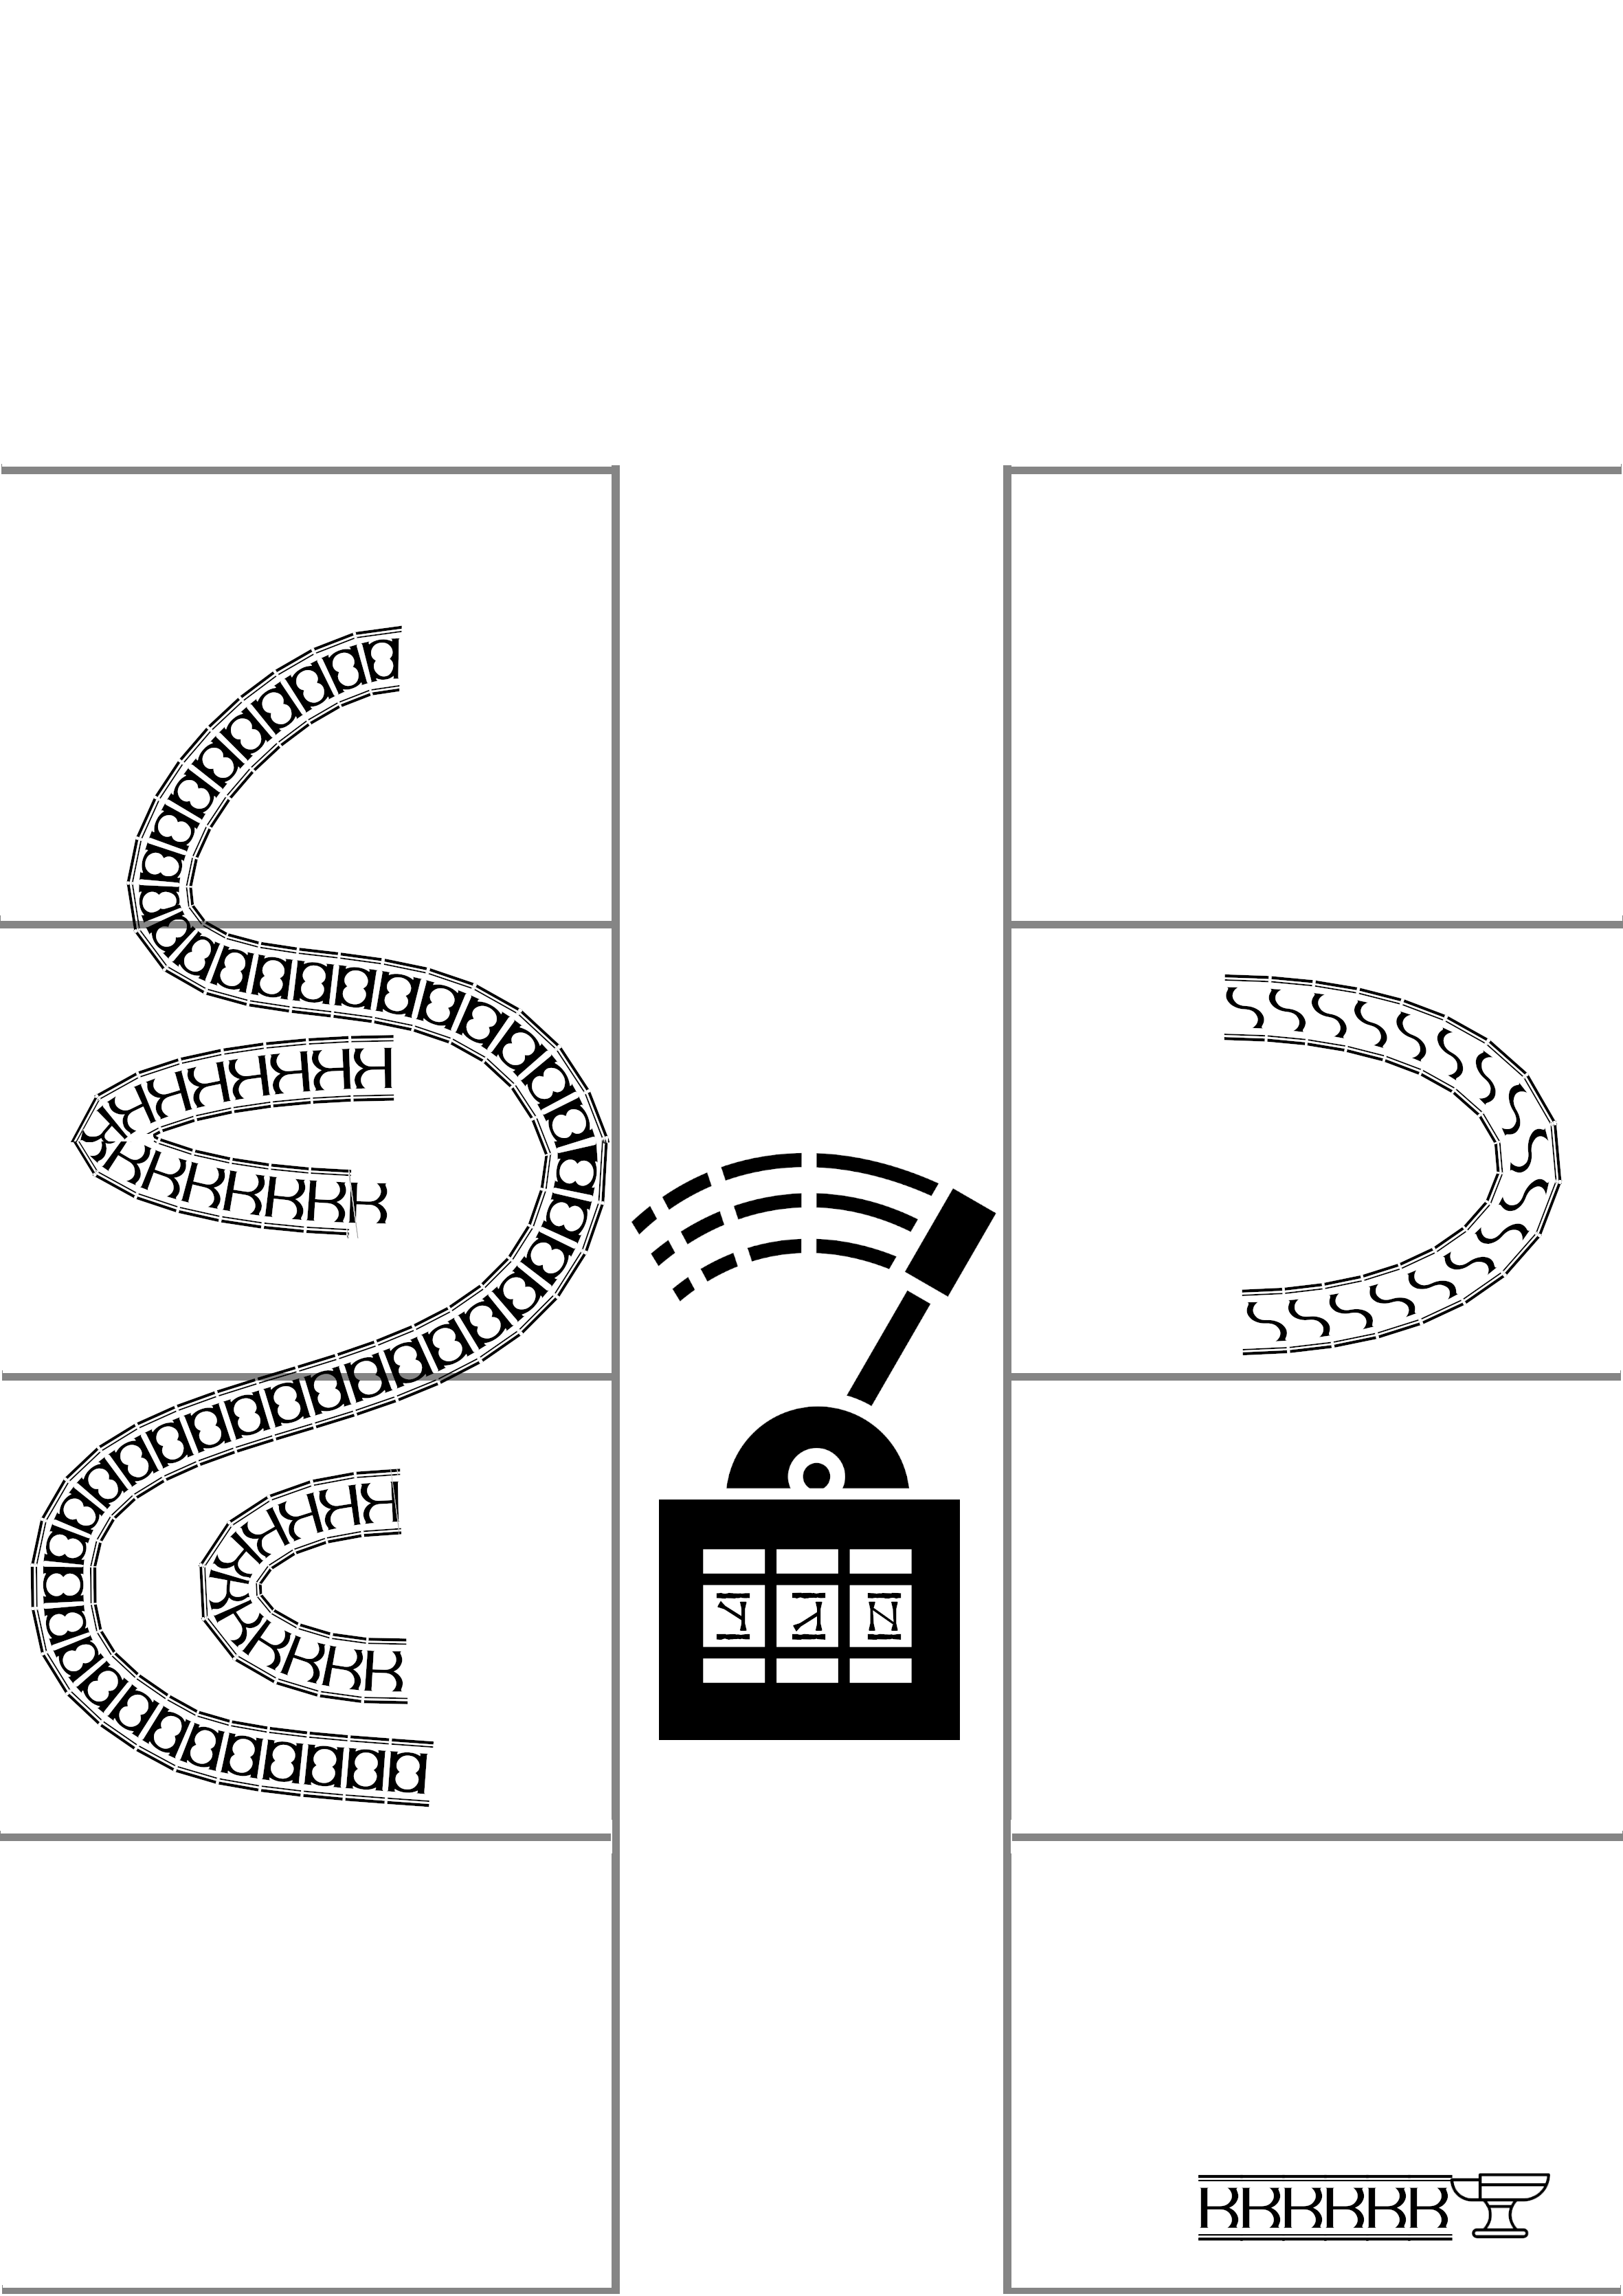
\includegraphics[width=0.95\textwidth]{tor-v.png}}
\newpage
\fbox{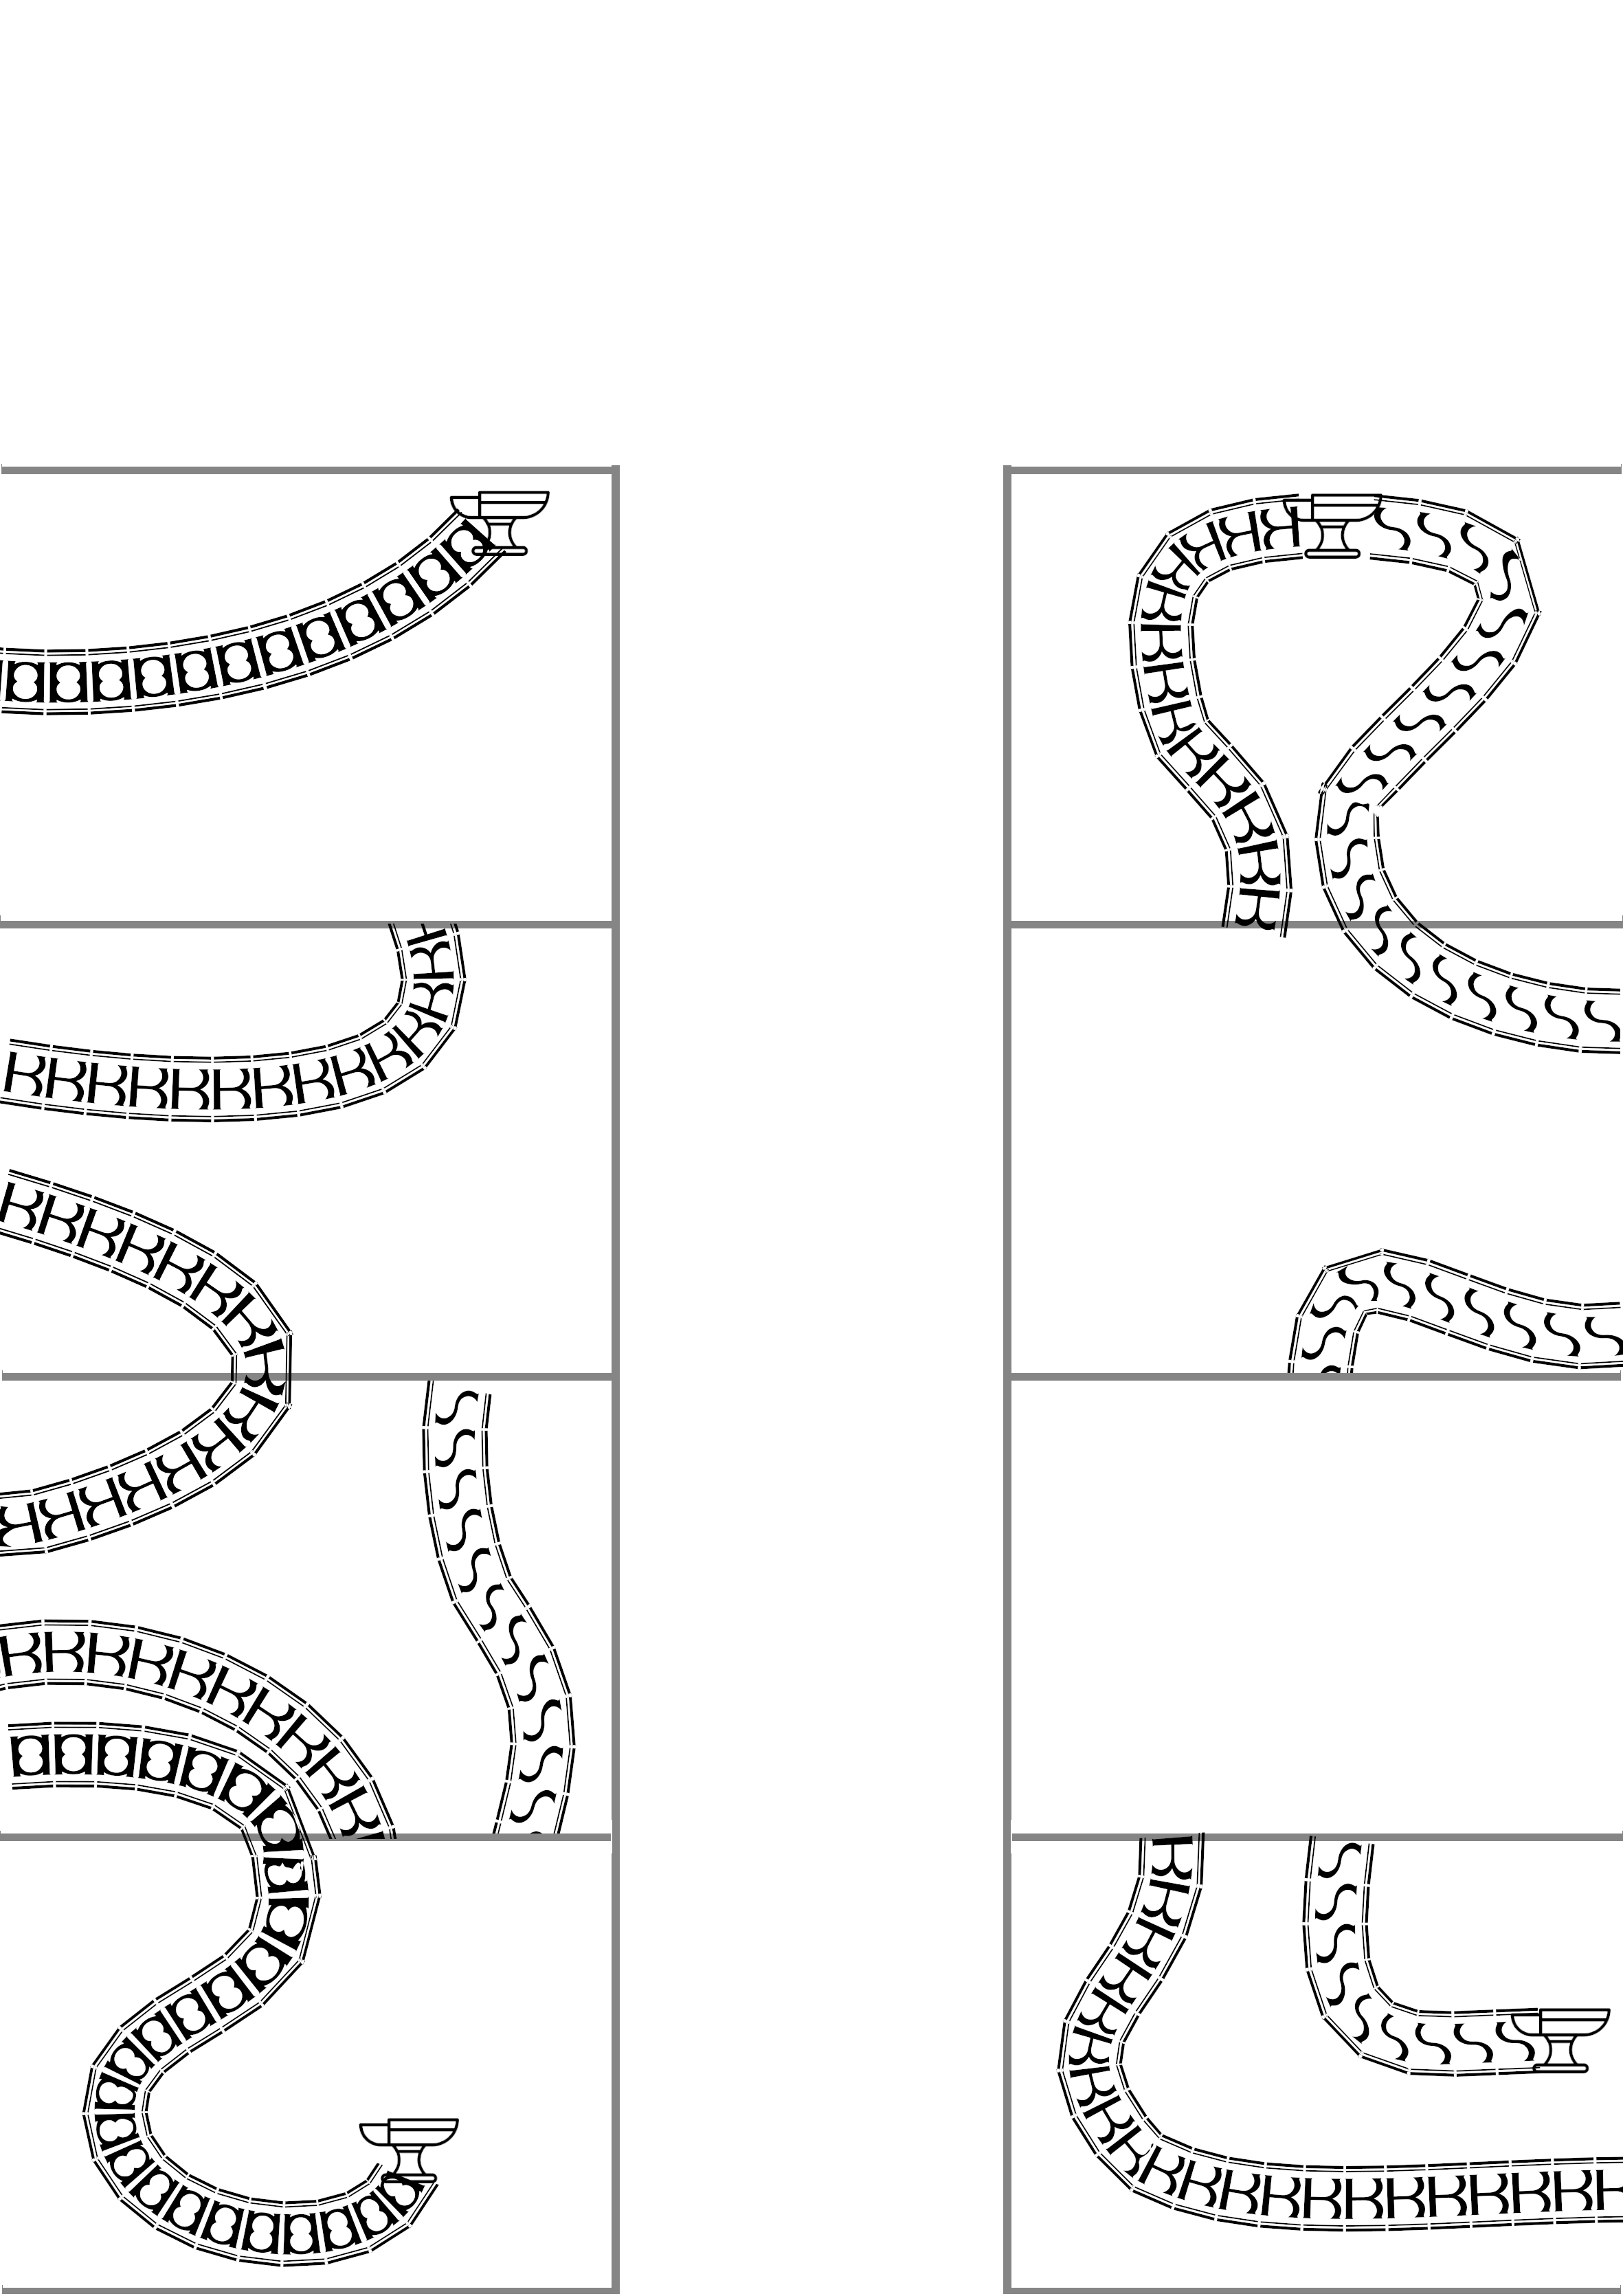
\includegraphics[width=0.95\textwidth]{tor-r.png}}
\handoutende
\spaltenanfang 
Des Rätsels Lösung ist somit \enquote{\textbf{Dorgrim}} -- Hochkönig und Träger des \textbf{Szepters der Stärke} während des \textbf{ersten Orkensturm}s.

Wird diese Kombination eingestellt und der Hebel gezogen, versinkt der mittlere Teil knirschend im Boden und es öffnet sich für einige Minuten ein schmaler Eingang.

Die Brücke steigt allmählich wieder auf ihre ursprüngliche Position, sobald der Hebel losgelassen wurde.
\subsubsection{Die Gruft}
\vorlesen{
	Auf der Innenseite der Tür gibt es einen zweiten Hebel, mit der sich der Ausgang ebenfalls öffnen lässt.
	
In der Mitte des Raums erinnert eine drei Schritt hohe Statue -- zugleich die tragende Säule -- an \textbf{Dorgrim \enquote{Orkenbrandt} Sohn des Dargalosch}.
Das steinerne Szepter in ihrer Hand hat eine Aussparung, in die das eigentliche Szepter hineinpasst. Diese ist jedoch leer.
\\
An den Wänden erinnern Platten an große Angehörige des \fkv s und ihre wichtigsten Taten.
In den Nischen darunter liegen jedoch nur Werkzeug und Waffen. Die Körper wurden dem Schöpfer \textbf{Angrosch} zurückgegeben und in den Feuerschlot geworfen.

Dieser \textbf{Schlot} kommt in Sicht, als ihr die Statue umrundet. Doch das feurige Glosen aus der Tiefe wird durch eine weitgehend transparente, wabernde Masse verzerrt.}

Eine \link{https://ilaris-online.de/app/kreatur/175}{Riesenamöbe} (\emph{Ilaris:105}) muss durch ein von den Wühlschraten gegrabenes Loch ihren Weg in die Gruft gefunden haben.
Zu den Dingen, die sie sich hier einverleibt hat, gehört ausgerechnet das Szepter!

\info{Die angegebenen Kampfwerte setzen voraus, dass die Gruppe durch die vorhergehenden Strapazen und Fallen schon einige \textit{Einschränkungen} aufweisen. Für eine ausgeruhte Gruppe ist die Amöbe kein ernst zu nehmender Gegner. Setzen Sie in diesem Fall die Werte für ein besonders gefährliches Exemplar ruhig ein wenig hinauf.}

\kreaturriesenamoebe

Nach dem Kampf kann die Gruppe dieses bergen. Es besteht hauptsächlich aus \textbf{Asthenil}, mit Applikationen aus \textbf{Toschkril} und \textbf{Zwergengold}.
Ein großer \textbf{Serpentin} ist an zentraler Stelle eingebettet.
\\
Auch einige Waffen und Werkzeuge finden sich in den amorphen Überresten der Amöbe. Diese sind natürlich von hervorragender Qualität (3xHQ und mehr, \emph{gutes Werkzeug} (\emph{Ilaris:61})), waren hier aber eigentlich zur ewigen Ruhe gebettet. Etwas mitzunehmen könnten Angrosch und auch Boron als Frevel auffassen \dots

\subsubsection{Immer diese Schrate!}
Beim Austritt aus der Gruft stellt sich heraus, dass die Wühlschrate während des Kampfes den Mechanismus der Brücke zerbissen haben. Sie bleibt dauerhaft abgesenkt.
\spaltenende
\probenkasten[bild=athletik,farbe=rot, gruppenprobe=nein, zusammenarbeit=nein, pw=24,
erfolg={Nach dem ersten Erfolg kann ein Seil herübergeworfen werden. Weitere Proben entfallen.},
misserfolg={Ein Fehlschlag führt bäuchlings auf die harte Oberfläche: W6+4~SP.},
]
{Akrobatik}{Der Sprung auf den Grat ist leicht. Schwer ist, punktgenau auf der schmalen und glatten Oberfläche zu landen. }
\spaltenanfang

\subsection{Weitere Ebenen}
Auf der Suche nach Abstiegen nehmen die Wühlschrat-Schäden zu. Auch muss hier und da an einer Schutthalde ein Durchschlupf gegraben werden.

Mit etwas Mühe finden sich aber Wege in die Tiefe, etwa zum großen Wasserspeicher, den \textbf{Felswandler} (\emph{KK:113}) bewachen, oder einem zugewachsenen Hinterausgang, wo vor Jahrhunderten Abraum entsorgt wurde.

Weitere Geheimnisse mögen sich hier verbergen, doch sind sie nicht Teil dieses Abenteuers.

\spaltenende

\neueseite

\section{Dritter\,Akt: Das Szepter}
\spaltenanfang
\subsection{Der Rückweg}
\label{zuruck}
\vorlesen{Als ihr das \textbf{Rattengold} passiert, fällt euch auf, dass der Brocken von der Mitte des Gangs verschwunden ist. Ihr seht euch um und findet stattdessen einen handtellergroßen goldenen \textbf{Knopf} von zwergischer Machart.}

\kasten{\textbf{Bonderik} ist ein Schurke, aber kein Anhänger des Namenlosen. Der Brocken ist auch für ihn sehr schwer und er hat sich beim Einpacken den Knopf abgerissen.}

Der natürliche Anlaufpunkt nach dem Fund des Szepters ist wieder Inradon \textbf{Xermosch}.
Für den nächsten Feuertag wird das Ritual angesetzt, das Szepter neu zu schmieden.
\subsection{Die Zeremonie}
\info{Stimmen Sie mit der Gruppe ab, von wo diese das Ritual miterleben wollen:
	Angroschgläubigen Figuren können daran mitzuwirken.
	Andere können ehrenhalber einen der begehrten Plätze im Tempel einnehmen. Wer sich irgendwann des Vertrauens des \fkvs als unwürdig erwiesen hat, wird wohl in der Halle ganz hinten stehen müssen -- ein interessanter Ausgangspunkt für die \emph{Verfolgungsjagd}.}
\vorlesen{%
Im Tempel ist jeder Platz besetzt. Auch in der großen Versammlungshalle sind hunderte, wenn nicht tausende Zwerginnen und Zwerge in ihren schönsten Kettenhemden zusammengekommen. Dicht gedrängt, murmeln sie seit Stunden gemeinsam Gebete in monotonem Singsang. Schließlich ist der große Moment da: Auf ein Zeichen von Inradon \textbf{Xermosch}, der im Portal des Tempels steht, werden Pauken und Ambosse geschlagen und unter einzelnen, tiefen Posaunenstößen wird das Szepter von einer Prozession in den Tempel getragen.

Dort ist ein Muffelofen aufgebaut worden, in dem die Metalle geläutert werden sollen.
Zahlreiche Beteiligte gehen dem Hohepriester zur Hand, darunter alle \textbf{Angrosch}-Geweihten des Finsterkamms und die meisten Mitglieder des \textbf{Tiefen Rats}. In jahrtausendealten steinernen Schalen fangen sie die geschmolzenen Metalle.
Der Inradon, den Serpentin in Händen, leitet sie zum großen Altar-Amboss. Danach greift er zum Hammer: \enquote{Mit diesen Schlägen werden wir unsere Zukunft in deine Hände legen, oh einziger Gott unseres Volkes.}
}

\subsubsection{Die Enttarnung des Bösewichts}

\probe{Wahrnehmung}{Wachsamkeit (16)}{\emph{keine Zusammenarbeit möglich.} Einer mitschmiedenden Figur fällt auf, dass das geschmolzene Zwergengold in einer der Schalen in Bewegung gerät.}

\kasten{Wer weiter entfernt steht oder bewusst versucht, den Knopf zuzuordnen, bemerkt mit derselben Probenschwierigkeit, dass die Knöpfe an Bonderiks Robe dem gefundenen gleichen.}

Genaueres Hinsehen zeigt, dass an Bonderiks Ärmel ein Knopf fehlt. Sobald sich ein Gruppenmitglied bemerkbar macht, erfasst Unruhe die Mitbetenden und setzt sich in der Menge fort, auch wenn die Ursache von den Wenigsten verstanden wird. \textbf{Xermosch} unterbricht das Ritual, um die Details zu erfragen.
\textbf{Bonderik} gerät nicht aus der Ruhe, tritt aber den Rückzug an.

Nun kann eine \emph{Verfolgungsjagd} (\emph{Ilaris:57}, DG\,3) beginnen:\\
In der dicht stehenden Menge ist die Grund-GS 1. \emph{Laufen} wäre \emph{langsam}.
Bonderik drängelt sich also durch die Menge und probt auf \emph{Körperkraft}, PW\,12, um \emph{schnell} voranzukommen. Er versucht, in die Hallen seiner Sippe zu gelangen und den verräterischen Rock loszuwerden.

Wer ihn verfolgt, kann ebenfalls \emph{KK} einsetzen, oder sich mit \emph{Akrobatik} über die Schultern (darüber einigermaßen empörter) Zwerg*innen bewegen. Die Grund-GS beträgt dann 4. Diesmal ist auch möglich, stattdessen die Menge auseinander zu treiben und den EW einer Probe auf \emph{Anführen} oder \emph{Einschüchtern} der Geschwindigkeit zuzuschlagen.\\
Wird die Verfolgungsjagd gewonnen, ist der Bösewicht gestellt und kann beschuldigt werden.
\textbf{Bonderik} streitet alles ab. Die Aussagen einiger Fremder und das Vorzeigen des Knopfs reichen als Beweis nur so weit, dass er sicherheitshalber vom Ritual ausgeschlossen wird. Anschließend werden die Metalle erneut getrennt und das Szepter ohne Rattengold geschmiedet. Nach einem letzten Gebet kreiselt es auf dem Altar, bis es auf \textbf{Garbalon} zeigt.\\
Nach dessen Krönung wird \textbf{Bonderik} unzufriedene Zwerge um sich scharen und in verlassenen Bauten im Süden des Finsterkamms ein neues Volk ausrufen.
\subsubsection{Und wenn nicht?}
Wenn die Gruppe die Manipulation nicht entdeckt, dann erleben sie eben ein einzigartiges Ritual mit, an dessen Ende \textbf{Bonderik} zum Hochkönig gewählt wird.
Entkommt er bei der Verfolgungsjagd, so fehlt ein Stück der Indizienkette und es ist die Gruppe, die wegen der Störung des Rituals von der restlichen Zeremonie ausgeschlossen wird.
Haben sie zuvor das Vertrauen des Inradon gewonnen, so wird dieser dennoch sicherheitshalber von vorn beginnen.
\subsection{Abgesang}
Für die Krönung wird auch \textbf{Gerambolosch} wieder hereingetragen.
Als die Krone das Haupt des neuen Hochkönigs berührt, erwacht der Bergkönig. (\enquote{Ich kehre aus dem Labyrinth meiner Träume zurück.}) Je nachdem segnet er seinen Sohn oder prophezeit dem Verräter Unglück.
\info{Eine hervorragende Gelegenheit für Sie, durch den Mund des greisen Königs eine Prophezeiung hinzuzufügen, die ihre Gruppe ins nächste Abenteuer führt.}
Dann schließt er die Augen für immer.

\spaltenende
\section{Anhang}
\spaltenanfang




\subsection{Finsterkoppen als Abenteuer\-schauplatz}

Das \fkv siedelt seit 3.000 Jahren im \textbf{Finsterkamm}; dies dürften in den meisten Familien rund 15~Generationen sein.

\subsubsection{Großling, sei auf der Hut}
Menschen sind in der Stadt \textbf{Finsterkoppen} äußerst selten zu Gast. Zwar unterhält das \fkv regen Handel über \textbf{Lowangen} und \textbf{Gashok}.
Dieser wird jedoch hauptsächlich über das deutlich leichter erreichbare \textbf{Hilltorp} abgewickelt.
Und auch der Weg über den \textbf{N\^orrnstieg} nach \textbf{Nordhag} fällt Kaufleuten aus Finsterkoppen deutlich leicht als umgekehrt.

Somit gibt es in Finsterkoppen schlechterdings kein Gebäude, das auf menschliche Maße ausgerichtet und keine Höhle, die für Menschen auskömmlich ausgeleuchtet wäre.

Selbst in prunkvollen Räumen wie der Versammlungshalle oder dem Angroschtempel herrscht \emph{Dämmerung} (\emph{Ilaris:38}).
Überall kann eine herabhängende Leuchte, ein Durchgang oder ein Sitzmöbel zum Hindernis für jemanden von mehr als sieben Spann Körpergröße werden.

\subsubsection{Das große Tor}
Es ist durchaus möglich, aus einigen der oberirdisch zugänglichen Gebäude in die Siedlung im Berginneren zu gelangen.
Diese Wege sind jedoch nicht öffentlich zugänglich, sondern führen in der Regel über Privatgemächer und Keller durch die Wohnhöhlen der ansässigen Sippen. 
(Außerdem haben diese Vorsorge getroffen, denn der Drache schläft nicht! Im Falle eines Angriffs lassen sich alle diese Zugänge mit wenigen Handgriffen zerstören.)

Der vorgesehene Weg führt durch das \textbf{große Tor}.
Dieses Wahrzeichen Finsterkoppens ist ein beeindruckendes Zeugnis zwergischer Baukunst:
Das ungeschulte Auge vermag nicht zu sagen, welcher Teil gewachsen, welcher gemeißelt, welcher gegossen und welcher gemauert worden sein mag.
Ein Gebirgsbach wurde so geleitet, dass die letzten Schritt zum Tor über eine Brücke führen, unter der schäumend das eiskalte Wasser tost.
Zwei Statuen von Heroen der Vorzeit in doppelter Lebensgröße halten als steinerne Wächter ewige Wacht.
Zwei lebendige Wächter, die deren Nachfahren sein könnten, warten vor dem äußersten der vier Torbögen.
Jeder dieser Bögen ist etwas kleiner als der nächste und  jeder enthält eine Vorrichtung zur Verteidigung gegen Drachen oder andere Angreifende:
\begin{enumerate}\setlength\itemsep {0em}
	\item Fallgatter,
	\item Schießscharten und Pechnasen sowie
	\item steinerne Torflügel, die auf Schienen geführt und mit einem System von Gegengewichten gesteuert, von einer einzigen Hand ins Schloss geführt werden, so dass kaum eine Fuge bleibt;
\end{enumerate}

An das Tor schließt sich ein etwa zwanzig Schritt langer Gang von acht Spann Höhe an.
Dieser führt direkt in die \textbf{große Versammlungshalle}.
Seine einzige Funktion ist, im Verteidigungsfall eine Engstelle zu bilden:
Sollten angreifende Drachen und Würmer das Tor tatsächlich überwinden, so lassen sie sich hier bekämpfen.

Historisch waren sowohl dieser Gang als auch die anschließende Halle und der \textbf{Angrosch}-Tempel in ihrer Verlängerung einst Teil des zentralen Einfuhr-Schachtes der ersten Mine von Finsterkoppen.
Der Gang wurde als Wehranlage verengt, die Halle zu Repräsentationszwecken vergrößert und der Tempel ausgebaut. 
Die Verlängerung dieses Schachtes in die Tiefe wurde durch eine steilere Treppe ersetzt und sein ursprünglicher Verlauf zu verschiedenen Zwecken umgebaut. Diese Höhlen werden im \emph{zweiten Akt} erkundet.

\subsubsection{Handwerk}
Wie bei allen zwergischen Völkern wird das Handwerk in hohen Ehren gehalten und die Bergleute, Mechaniker*innen, vor allem aber die Schmiedewerkstätten bringen Ergebnisse hervor, die für die meisten Menschen unerreichbar bleiben. \textbf{Ogrim Sohn des Olgosch}, \textbf{Arombolosch Eisenarm} oder \textbf{Xagula, Tochter der Xebrima} wären unter Umständen auch bereit, einem Menschen eine Waffe zu verkaufen.
Sie als Lehrmeister*innen zu gewinnen, setzt dagegen für nichtzwergische Figuren einen großen Verdienst voraus (wie ihn dieses Abenteuer darstellen kann).

Unter Fachleuten berühmt ist auch \textbf{Gandrasch Sohn des Gengram}. Der geniale, aber leicht abzulenkende Tüftler ist dafür zuständig, die Geschütze und andere mechanische Verteidigungsanlagen für das \fkv zu warten.
In seiner wenigen freien Zeit bastelt er am liebsten an Armbrüsten und hat schon manch eine Verbesserung zu Stande gebracht -- ebenso wie eigenwillige Einzelstücke.


\subsubsection{Truppen}

Das \fkv ist immer von Feinden umgeben gewesen und es wird allseits erwartet, dass alle Erwachsenen im Fall des Falles eine Axt nicht nur zu schmieden, sondern auch zu führen verstehen.

Daneben hat das Bergkönigreich einige erfahrende \textbf{Kämpfer*innen}, die regelmäßig Hatz auf \textbf{Tatzelwürmer} und \textbf{Horndrachen} oder Orksippen planen,
die für die Siedlungen oder Siedlungsvorhaben der Zwerge zur Gefahr werden.
Die Wachdienste in Finsterkoppen selbst -- einschließlich der Wache am großen Tor -- sind jedoch so auf die Sippen verteilt,
so dass alle mal für einen Mond dran sind.
Angesichts der relativ friedlichen letzten Jahrhunderte sind diese Wachen vor allem durch ihre ausgezeichnete Ausrüstung gefährlich -- weniger, weil sie nach einer Gelegenheit suchen, diese einzusetzen.

\subsubsection{Gasthäuser}
In Finsterkoppen gibt es drei \textbf{Tavernen}: 
\begin{enumerate}
\item \textbf{\enquote{Bei Schwarzbart}} -- hier verkehren auch Jugendliche vor der Feuertaufe --,
\item \textbf{\enquote{Rote Erde}}, wo \textbf{Dragoran Sohn des Denderan} vor allem Bergleute begrüßt und \item \textbf{\enquote{Hammer und Amboss}} von Wirt \textbf{Vothan Dengeler} -- wo mehr Handwerker*innen anzutreffen sind.
\end{enumerate}

\subsubsection{Heiler}
Wer an Krankheiten leidet oder zahlreiche Wunden zählt, kann den \textbf{Heiler Thoram Sohn der Cadrima} aufsuchen.
Allerdings ist auch dieser auf zwergische Anatomie spezialisiert und wird den ein oder anderen Fluch, wie viel Verbandsmaterial auf weiches Großling-Fleisch verwendet werden muss, nicht unterdrücken können.

Wer jeglichem Aberglauben abhold ist, kann sein Glück auch bei \textbf{Turgol} suchen, dem Berater des Bergkönigs, der sich in letzter Zeit besonders häufig in der Stadt aufhält.
Von der Bevölkerung wird dieser Name allerdings meist nur gemurmelt und von einem Besuch abgeraten.
Noch weniger als seine Hilfe in Anspruch nehmen würden sie jedoch ein wirklich schlechtes Wort sagen -- so sehr ängstigt sie allein der Gedanke an den (eigentlich sehr gutwilligen) Geoden.

\subsubsection{Sonstige Besonderheiten}
An den Hängen der umliegenden Berge grasen \textbf{Ponys}, die unter Tage Maschinen für den Bergbau betreiben. Die Monde von Hesinde bis Tsa verbringen sie in Stallhöhlen.


\subsubsection{Weitere wichtige Bewohner}

Die Beschreibung der Mitglieder des \textbf{Tiefen Rat}s finden Sie im \emph{ersten Akt} auf S.\,\pageref{rat}. 

\bigskip

\textbf{Muragolosch}

Der Schüler \textbf{Turgol}s schlägt im Wesen nicht nach dem gutmütigen Sumudiener, sondern hat sich dem Element Eis zugewandt.
Seit Jahrzehnten wächst seine Verachtung für andere Völker.
Er ist einer der wenigen Vertrauten \textbf{Bonderik}s und vergiftet in seinem Auftrag Bergkönig \textbf{Gerambolosch} in seinen (beklagenswerten, aber beschwiegenen) Zustand.

Falls die Gruppe auf diese Spur stößt, kann \textbf{Muragolosch} eine größere Rolle spielen. Im unwahrscheinlichen Fall eines Kampfes gegen \textbf{Bonderik} kann er als Joker eingreifen und diesen mit Zaubern wie \biglittlecap{Weg durch Sumus Leib} in Sicherheit bringen.

\bigskip

\textbf{Arglescha Tochter der Angrarda}

Die Tochter \textbf{Garbalon}s ist erst ein halbes Jahrhundert alt, gilt aber dennoch schon jetzt als eine der besten Kämpferinnen im \fkv.
Jüngst zeigt sie Interesse, auch ihre Fähigkeiten als Anführerin auszubauen -- ein Vorhaben, das durch die Wahl ihres Vaters zum Bergkönig noch plausibler wird.

Arglescha eignet sich hervorragend als romantisches Interesse für einen Zwergenkavalier als Spielerfigur.

\spaltenende
\begin{center}
\zeichnung[0.95\textwidth]{zwerg.JPG}
\end{center}

\newpage
%\subsection{Beispiel-Charaktere}
%\paragraph{Graboxa, Zwergische Angrosch-Geweihte, Hüterin der Wacht}
%\paragraph{Dascha, Gjalsker Tierkriegerin}
%\paragraph{Jasinthe, Garether Gelehrte}
%\paragraph{Odir Sensendengler, Abenteurer und Pferdedieb}
\subsection{Szenen/Eigenheiten-Tabelle}
Hier eine Übersichts-Tabelle, mit welchen Eigenheiten Sie den Figuren in welcher Szene \emph{das Leben schwer machen} \emph{(Ilaris:15)} können, um Schicksalspunkte zu verteilen:

\begin{tabularx}{0.98\linewidth}{l|XXX}
	&\tkopf{Der Tiefe Rat} & \tkopf{Die Finsterkopp-Binge}&\tkopf{Das Szepter}\\
	\hline
	
	\textbf{Graboxa}&\textbf{Alter bringt Weisheit}\newline Graboxa könnte sich einer im Rat geäußerten Meinung einfach deswegen anschließen, weil sie von einer deutlich älteren Person kommt. Bieten Sie einen Schicksalspunkt, wenn daraus Spannungen mit der Gruppe entstehen.
	&\textbf{Für Angrosch!}\newline Graboxa empfindet unmittelbar den Frevel, die Artefakte nicht wieder in die zugehörigen Nischen zu legen. Gönnen Sie ihr einen Schicksalspunkt, wenn sie die anderen davon überzeugt, auf diese handfeste Belohnung zu verzichten.
	& \textbf{Drachendiener überall}\newline Warum hat der Hohepriester beim Gebet die Einzigkeit des Gottes so betont? Und warum hat er ihn nicht beim Namen genannt?? Eine vorübergehende Verwirrung kurz vor Schluss darüber, wer hier (eigentlich) alles Übles im Schilde führt, gibt einen Schicksalspunkt.\\
	
	\textbf{Dascha}&\textbf{Gewalt ist immer eine Lösung}\newline Wenn Dascha vorschlägt, den greisen Bergkönig einfach zu erschlagen, ist das schon einen Schicksalspunkt wert -- selbst dann, wenn es der Gruppe gelingt, sich auf einen Übersetzungsfehler rauszureden. &\textbf{Singender Stahl}\newline Für Dascha ist es ein Unding, die hervorragenden Äxte einfach allesamt in der Gruft liegen zu lassen. Gönnen Sie ihr einen Schicksalspunkt, wenn sie sich darüber mit Graboxa überwirft.&\textbf{Trolltochter}\linebreak Bei Daschas Größe ist nicht die Frage, ob sie sich den Kopf stößt, sondern wie oft \dots\ Während der Verfolgungsjagd kann Dascha für einen Schicksalspunkt auf einen Würfelwurf verzichten und den Vergleich verlieren.\\
	
	\textbf{Jasinthe}&\textbf{Wisst ihr eigentlich \dots ?}\newline Wenn den Rat eine Sache nicht interessiert, dann wie die Eslamiden eine ähnliche Situation gelöst haben. Für eine peinlich-weitschweifige Erklärung könnte es einen Schicksalspunkt geben.&\textbf{Wunder der Technik}\newline Wenn Jasinthe begeistert darauf eingeht, wie gut die zwergische Technik auch nach Jahrhunderten ohne Pflege noch funktioniert und dabei als erste in die Bolzenfalle tritt, gibt es einen Schicksalspunkt.&\textbf{Chronistin}\newline Nein, der Hohepriester möchte nicht die vorige Strophe des Gebets noch einmal wiederholen, damit es mitgeschrieben werden kann. Ob wir jetzt endlich mit dem heiligen Ritual fortfahren können \dots?\\
	
	\textbf{Odir}&\textbf{Baliho? Nie dagewesen \dots}\newline Ein Lederwaren-Händler will in Odir einen Mann erkennen, der beim Pferdemarkt in Baliho am Pranger stand. Es braucht einigen Aufwand, ihn vom Gegenteil (\enquote{Menschen sehen doch alle gleich aus!}) zu überzeugen.&\textbf{Wo ist meine Hasenpfote?}\newline Dass die Wühlschrate Lichtquellen stehlen, ist das eine. Aber dass sie dabei auch den Glücksbringer haben mitgehen lassen! Die Suche nach dem Szepter muss sofort unterbrochen werden. Was ist ein Szepter gegen die Hasenpfote?!&\textbf{Gold, was glänzt}\newline Einerseits ist der goldene Knopf ein wichtiges Indiz, andererseits ist er auch einiges wert. Wenn Odir eindringlich andere -- schlechtere -- Wege der Anklage sucht, um den Knopf behalten zu können, kann das mit einem Schicksalspunkt belohnt werden.\\

\end{tabularx}


\neueseite

\handout
\subsection{Das Relief hinter dem Angrosch-Altar}
%Lösung: D G M
\label{karten}
\mbox{}

\begin{center}
	\bigskip
	\vfill
	
\includegraphics[width=0.5\textwidth]{ngrsch.png}
\end{center}

\vfill

\begin{multicols}{3}
	\karte{
		\begin{multicols}{3}\mbox{ }\linebreak \begin{tabularx}{1.5cm}{|X|}
				\leer \leer \amboss \amboss
				\hline	\end{tabularx}	\neuespalte
			\begin{center} \mbox{ } \linebreak[4]
				
\includegraphics[width=\columnwidth]{S.png}
			\end{center} \neuespalte \mbox{ } \begin{tabularx}{1.5cm}{|X|}
				\amboss \leer \leer \leer
				\hline \end{tabularx} \end{multicols}
	}\vfill
	
	\karte{
		\begin{multicols}{3}\mbox{ }\linebreak \begin{tabularx}{1.5cm}{|X|}
				\amboss \leer \amboss \leer
				\hline	\end{tabularx}	\neuespalte
			\begin{center} \mbox{ } \linebreak[4]
				
\includegraphics[width=\columnwidth]{B.png}
			\end{center} \neuespalte \mbox{ } \begin{tabularx}{1.5cm}{|X|}
				\leer \amboss \leer \amboss
				\hline \end{tabularx} \end{multicols}
	}\bigskip
	
	\karte{
		\begin{multicols}{3}\mbox{ }\linebreak \begin{tabularx}{1.5cm}{|X|}
				\amboss \leer \leer \amboss
				\hline	\end{tabularx}	\neuespalte
			\begin{center} \mbox{ } \linebreak[4]
				
\includegraphics[width=\columnwidth]{G.png}
			\end{center} \neuespalte \mbox{ } \begin{tabularx}{1.5cm}{|X|}
				\leer \amboss \amboss \leer
				\hline \end{tabularx} \end{multicols}
	}\bigskip
	
	
	\karte{
		\begin{multicols}{3}\mbox{ }\linebreak \begin{tabularx}{1.5cm}{|X|}
				\amboss  \amboss \leer \leer
				\hline	\end{tabularx}	\neuespalte
			\begin{center} \mbox{ } \linebreak[4]
				
\includegraphics[width=\columnwidth]{N.png}
			\end{center} \neuespalte \mbox{ } \begin{tabularx}{1.5cm}{|X|}
				\leer  \leer \leer \leer
				\hline \end{tabularx} \end{multicols}
	}\bigskip
	
	\karte{
		\begin{multicols}{3}\mbox{ }\linebreak \begin{tabularx}{1.5cm}{|X|}
				\leer \leer \leer \amboss
				\hline	\end{tabularx}	\neuespalte
			\begin{center} \mbox{ } \linebreak[4]
				
\includegraphics[width=\columnwidth]{F.png}
			\end{center} \neuespalte \mbox{ } \begin{tabularx}{1.5cm}{|X|}
				\amboss  \amboss \amboss \leer 
				\hline \end{tabularx} \end{multicols}
	}\bigskip
	
	\karte{
		\begin{multicols}{3}\mbox{ }\linebreak \begin{tabularx}{1.5cm}{|X|}
				\leer \amboss \amboss \amboss
				\hline	\end{tabularx}	\neuespalte
			\begin{center} \mbox{ } \linebreak[4]
				
\includegraphics[width=\columnwidth]{J.png}
			\end{center} \neuespalte \mbox{ } \begin{tabularx}{1.5cm}{|X|}
				\amboss \leer \leer \leer
				\hline \end{tabularx} \end{multicols}
	}\bigskip

	
	\karte{
		\begin{multicols}{3}\mbox{ }\linebreak \begin{tabularx}{1.5cm}{|X|}
				\leer \leer \leer  \amboss
				\hline	\end{tabularx}	\neuespalte
			\begin{center} \mbox{ } \linebreak[4]
				
\includegraphics[width=\columnwidth]{H.png}
			\end{center} \neuespalte \mbox{ } \begin{tabularx}{1.5cm}{|X|}
				\amboss \amboss \leer \leer
				\hline \end{tabularx} \end{multicols}
	}\bigskip
	
	\karte{
		\begin{multicols}{3}\mbox{ }\linebreak \begin{tabularx}{1.5cm}{|X|}
				\leer \amboss \amboss \leer
				\hline	\end{tabularx}	\neuespalte
			\begin{center} \mbox{ } \linebreak[4]
				
\includegraphics[width=\columnwidth]{P.png}
			\end{center} \neuespalte \mbox{ } \begin{tabularx}{1.5cm}{|X|}
				\amboss \leer \leer \leer
				\hline \end{tabularx} \end{multicols}
	}\bigskip
	
	\karte{
		\begin{multicols}{3}\mbox{ }\linebreak \begin{tabularx}{1.5cm}{|X|}
				\leer \leer \leer \leer
				\hline	\end{tabularx}	\neuespalte
			\begin{center} \mbox{ } \linebreak[4]
				
\includegraphics[width=\columnwidth]{D.png}
			\end{center} \neuespalte \mbox{ } \begin{tabularx}{1.5cm}{|X|}
				\amboss \leer \amboss \amboss
				\hline \end{tabularx} \end{multicols}
	}\bigskip
	
	
	\karte{
		\begin{multicols}{3}\mbox{ }\linebreak \begin{tabularx}{1.5cm}{|X|}
				\leer \amboss \leer \amboss
				\hline	\end{tabularx}	\neuespalte
			\begin{center} \mbox{ } \linebreak[4]
				
\includegraphics[width=\columnwidth]{W.png}
			\end{center} \neuespalte \mbox{ } \begin{tabularx}{1.5cm}{|X|}
				\leer \leer \leer \leer
				\hline \end{tabularx} \end{multicols}
	}\bigskip
	
	
	\karte{
		\begin{multicols}{3}\mbox{ }\linebreak \begin{tabularx}{1.5cm}{|X|}
				\leer \amboss \amboss \amboss
				\hline	\end{tabularx}	\neuespalte
			\begin{center} \mbox{ } \linebreak[4]
				
\includegraphics[width=\columnwidth]{R.png}
			\end{center} \neuespalte \mbox{ } \begin{tabularx}{1.5cm}{|X|}
				\leer \leer \leer \leer
				\hline \end{tabularx} \end{multicols}
	}\bigskip
	
	\karte{
		\begin{multicols}{3}\mbox{ }\linebreak \begin{tabularx}{1.5cm}{|X|}
				\amboss \amboss \leer \amboss
				\hline	\end{tabularx}	\neuespalte
			\begin{center} \mbox{ } \linebreak[4]
				
\includegraphics[width=\columnwidth]{M.png}
			\end{center} \neuespalte \mbox{ } \begin{tabularx}{1.5cm}{|X|}
				\leer \leer \amboss \leer
				\hline \end{tabularx} \end{multicols}
	}\bigskip
	
\end{multicols}
\vfill
\footnotesize
\textbf{Lizenzhinweise:}
\label{lizenz}
\bigskip

Rogolan-Font von Thorsten Most auf Basis der Spielhilfe \enquote{Angroschs Kinder}.

Ambosssymbole: Anvil Impact von Lorc, \href{https://game-icons.net/1x1/lorc/anvil-impact.html}{game-icons.net} unter der \href{https://creativecommons.org/licenses/by/3.0/}{CC BY 3.0-Lizenz}.

Hebel-Symbol: Lever icon von Lorc, \href{https://game-icons.net/1x1/lorc/lever.html}{game-icons.net}{CC BY 3.0-Lizenz}.
\normalsize



\kapitel{Spielhilfen}
\section{Neue Entwicklungen bei den Spielhilfen}
\credit{Autor}{Alrik Normalpaktierer}
\spaltenanfang
Im \link{https://dsaforum.de/app.php/dlext/details?df_id=416}{ersten Band der Chroniken von Ilaris}
hatten wir neben neuen Spielhilfen (wie der ersten Version der Manöverkarten, einigen Tipps zum Abenteuervorbereiten, \dots) auch einen Überblick über kostenfreien Spielhilfen zusammengestellt, die den Einstieg in Ilaris vereinfachen.
Diese Übersicht ist immer noch hilfreich, aber vom Stand Früh\-som\-mer 2022.
Da die Entwicklung vieler Projekte weitergelaufen ist, nicht mehr in allen Punkten aktuell.
Inzwischen bietet \link{https://ilaris-online.de/app/inhalte/}{Ilaris Online} eine vollständige Liste, filter- und sortierbar nach Kategorien. Damit ergänzt die Website das Angebot des gesamten Ilaris-Regelwerks als Datenbank.

Im Folgenden wollen wir einige ausgewählte Spielhilfen detaillierter vorstellen.

\subsection*{Generierungsprogramm Sephrasto}
\link{https://github.com/Aeolitus/Sephrasto/releases}{Sephrasto} hat in den letzten Jahren erneut eine deutliche Weiterentwicklung durchlaufen und liegt inzwischen in der Version 5 vor.

\begin{itemize}
\item Vollumfassende regelkonforme Charaktererstellung und -steigerung mit zahlreichen Hilfestellungen
\item 	Assistent für die Erstellung neuer Charaktere
\item	Speichermöglichkeit und PDF-Export
\item	Automatisch erstellter PDF-Anhang mit allen für den Charakter relevanten Regeln
\item	Vier verschiedene Charakterbögen zur Auswahl, auch eigene sind möglich
\item	Umfassende Unterstützung für Hausregeln durch einen ins Programm integrierten Datenbankeditor. Hausregeln können so auch einfach gespeichert und geteilt werden.
\item	Sephrasto unterstützt Plugins. Sie lassen sich aus dem Programm heraus installieren und (de-)aktivieren.
Zahlreiche von der Community erstellte Plugins -- z.\,B. das Manöverkarten-Tool (s.\,u.) und ein Exporter für Foundry-VTT -- stehen zur Verfügung.
\item	Grafische Darstellung über Schriftarten und -größen und Themes leicht anpassbar
\item	In-App-Hilfe
\end{itemize}

\zeichnung[0.8\columnwidth]{Curthan2.jpg}



\subsection*{Manöverkarten}
Eines der Plugins erlaubt, einen Satz Manöverkarten passend zur jeweiligen Figur zu erstellen.
Dazu gehören die verfügbaren Manöver im Kampf und praktische Regelübersichten.
Auch der Regeltext aller Zauber und Liturgien liegen dabei auf jeweils einer Karte mit sprechenden Symbolen vor.
So erhältst du bereits mit dem Erstellen deines Charakterbogens deine Optionen im Spiel druckfertig in übersichtlicher Form.

\subsection*{Kreaturendatenbank}
Auch die \link{https://ilaris-tools.github.io/IlarisDB/db/kreaturen/}{Kreaturen\-datenbank} wurde erheblich weiterentwickelt.
Sie umfasst neben allen Kreaturen des Regelwerks inzwischen auch viele Gegner und NSCs, die andere Spielleitungen in ihrer Vorbereitung erstellt haben.
Spielwerte stehen so als Konvertierungen für Abenteuer anderer Regeleditionen zur Verfügung.

Angemeldete Nutzende können selbst Kreaturen eintragen und sie für FoundryVTT oder als LaTeX- oder als Brauerei-Code (s.\,u.) im Format einer Manöverkarte exportieren.

%In der Ausarbeitung eigener Szenarien oder der Vorbereitung des Spielabends ist die stets überarbeitete Spielleitung für folgende Hilfestellungen dankbar:
%
%\tabelle{p{1.9cm}|p{1cm} X X X}{
%	
%	\tkopf{Spielhilfe} & \tkopf{von} & \tkopf{Was ist das?} &\tkopf{Wobei hilft es?}  \\
%	\hline
%	
%	\link{https://ilaris-tools.github.io/IlarisDB/db/kreaturen/}{Kreaturen\-datenbank}&Lukas Ruhe&Eine Datenbank mit den Spielwerten aus dem Bestiarium und vielen Hausregeln.&Schnell Spielwerte nachzuschlagen und zu kopieren.\\
%	%		\item CharakterToText
%	
%	\hline
%}

\subsection*{Layout: Die Brauerei}


%\tabelle{p{3cm}|p{2.5cm} X }{
%	\tkopf{Spielhilfe} & \tkopf{von} & \tkopf{Was ist das?} \\
%	\hline
%	
%\link{https://github.com/Ilaris-Tools/IlarisTex}{IlarisTex}&Lukas Ruhe&\LaTeX-Klasse, die zahlreiche Gestaltungselemente zur Verfügung stellt.\\
%
%\link{https://www.dropbox.com/sh/xs1w5r4rq3m0a99/AAB2MGJvEr0O8uxG4_9USVpQa?dl=0}{Ilaris-Artwork}&Bernhard Eisner&Symbole und Illustrationen aus dem Ilaris-Regelbuch.\\
%
%\link{https://webzine.nandurion.de/2013/10/15/dsa-schriftartenpaket-stand-022011/}{Schriftarten-Paket}&Salaza&Digitale Fonts für verschiedene aventurische Schriften.\\
%\hline
%}
\spaltenende

\newpage

\section{Encounter-Design}


\newcommand{\kreaturhummeriersoldat}{\kreatur{Hummerier Soldat}{Schreckliche Ausgeburt der endlosen Tiefen, großer Gegner}{gfx/kreaturen/mythen}{\kreaturkampfwerte{6/11}{9}{2/5 (Land/Wasser)}{4}\trennlinie \kreaturvorteile{Angepasst IV (Wasser), Natürliche Rüstung, Amphibisch}\trennlinie \kreaturwaffe{Scheren}{0}{10}{10}{3W6+2}{Doppelangriff, Rüstungsbrecher, Umklammern (-4)}\kreaturwaffe{Partisane}{2}{11}{11}{3W6+7}{}\kreaturkampfvorteile{Kraftvoller Kampf II, Ausfall, Offensiver Kampfstil, Niederwerfen, Hammerschlag}\trennlinie \kreaturattribute{CH 4, FF 2, GE 4, IN 8, KK 16, KL 6, KO 16, MU 10}\kreaturfertigkeiten{Einschüchtern 12, Wachsamkeit 6, Zähigkeit 14}\kreaturinfo{Profane Vorteile}{Abgehärtet I\&II, Schnelle Heilung, Muskelprotz, Zerstörerisch II, Willensstark I}}}
%\trennlinie \kreaturinfo{Quelle}{\href{https://dsaforum.de/download/file.php?id=14259}{Krustentiere}}}


\newcommand{\kreaturhummerierelementarist}{\kreatur{Hummerier Elementarist}{Gebieter des Unwassers, 'Artillerie' der Hummerier. Großer Gegner.}{gfx/kreaturen/mythen}{\kreaturkampfwerte{5/9}{14}{2/5 (Land/Wasser)}{4}\trennlinie \kreaturvorteile{Angepasst IV (Wasser), Natürliche Rüstung, Amphibisch}\trennlinie \kreaturwaffe{Scheren}{0}{8}{8}{3W6}{Doppelangriff, Rüstungsbrecher, Umklammern (-4)}\kreaturwaffe{Spieß}{2}{10}{10}{3W6+2}{}\trennlinie \kreaturattribute{CH 16, FF 2, GE 4, IN 8, KK 14, KL 16, KO 12, MU 16}\kreaturfertigkeiten{Autorität (alle) 16, Wachsamkeit 12, Zähigkeit 12, Elementarkunde 14, Geschichten und Legenden 12}\kreaturinfo{Profane Vorteile}{Abgehärtet I, Schnelle Heilung, Willensstark I+II}\trennlinie \kreaturinfo{AsP}{52}\kreaturinfo{(Un-)Wasser}{17 (Aquasphaero, Herbeirufung des Wassers, Wasserwand, Leib der Wogen, Mahlstrom, Zorn der Elemente)}\kreaturinfo{Magische Vorteile}{Gefäß der Sterne, Verbotene Pforten, Astrale Regeneration, verbesserte  Astrale Regeneration, Bändiger der Elemente, Meister der Wünsche, Kraftlinienmagie, Effezientes Zaubern, Tradition der Hummerier III (Wasserzauber 1x MM extra, ermöglicht Zeit lassen)}}}

\newcommand{\kreaturhummerierpriesterkrustentiere}{\kreatur{Hummerier Priester}{Anführer und Veteran der Truppen der tiefen Tochter. Paktierer. Großer Gegner.}{gfx/kreaturen/mythen}{\kreaturkampfwerte{8/14}{14}{2/5 (Land/Wasser)}{4}\trennlinie \kreaturvorteile{Angepasst IV (Wasser), Natürliche Rüstung, Amphibisch, Paktierer III}\trennlinie \kreaturwaffe{Scheren}{0}{12}{12}{3W6+3}{Doppelangriff, Rüstungsbrecher, Umklammern (-4)}\kreaturwaffe{Partisane}{2}{11}{11}{3W6+8}{}\kreaturkampfvorteile{Kraftvoller Kampf III, Ausfall, Offensiver Kampfstil, Niederwerfen, Hammerschlag}\trennlinie \kreaturattribute{CH 18, FF 2, GE 4, IN 8, KK 18, KL 10, KO 18, MU 18}\kreaturfertigkeiten{Autorität (alle) 18, Wachsamkeit 10, Zähigkeit 18, Götter und Kulte 12}\kreaturinfo{Profane Vorteile}{Abgehärtet I\&II, Schnelle Heilung, Muskelprotz, Zerstörerisch I+II, Willensstark I+II, Haltet Stand!, Keine Gefangenen!}\trennlinie \kreaturinfo{GuP}{28}\kreaturinfo{Dämonische Hilfe}{15 (Dämonische Stärkung (Derekunde, KO, MU), Meister der Maritimen, Gebieter der Gezeiten, Ertränken)}\kreaturinfo{Karmale Vorteile}{Erzdämonische Tradition III, Dämonische Waffe (wie gesegnete Waffe)}}}

\newcommand{\kreaturhummerierleibgarde}{\kreatur{Hummerier Leibgarde}{Hummerischer Elitekrieger und Beschützer, großer Gegner}{gfx/kreaturen/mythen}{\kreaturkampfwerte{6/11}{14}{3}{10}\trennlinie \kreaturvorteile{Angepasst IV (Wasser), Natürliche Rüstung, Amphibisch}\trennlinie \kreaturwaffe{Schere}{0}{17}{14}{3W6}{Rüstungsbrecher, Umklammern (-4)}\kreaturwaffe{Partisane}{2}{17}{14}{3W6+5}{}\kreaturwaffe{Scherenschild}{0}{17}{14}{1W6+4}{}\kreaturkampfvorteile{Schildkampf III, Ausfall, Offensiver Kampfstil, Defensiver Kampfstil, Gegenhalten, Niederwerfen, Hammerschlag}\trennlinie \kreaturattribute{CH 8, FF 2, GE 4, IN 12, KK 16, KL 6, KO 16, MU 16}\kreaturfertigkeiten{Einschüchtern 14, Wachsamkeit 11, Zähigkeit 16}\kreaturinfo{Profane Vorteile}{Abgehärtet I\&II, Schnelle Heilung, Muskelprotz, Zerstörerisch I+II, Willensstark I+II}}}

\newcommand{\kreaturkrabbenschwarm}{\kreatur{Krabbenschwarm}{Schwarm von winzigen Krabben. Großer Gegner}{gfx/kreaturen/daimonid}{\kreaturkampfwerte{1, Koloss I}{1 (für ein einzelnes Tier)}{2}{1}\trennlinie \kreaturvorteile{Angepasst IV (Wasser), Amphibisch, Schmerzimmun II, Verwundbarkeit IV (Flächenschaden), Wundblockade (s.u.) . }\trennlinie \kreaturwaffe{Scherenschnitte}{0}{10}{10}{1W6+3}{}\kreaturkampfvorteile{Zusätzliche Attacke I, Immunität (Niederwerfen, Umreißen, u.ä.)}\trennlinie \kreaturfertigkeiten{Wachsamkeit 16, Pirschen 16}\trennlinie \kreaturinfo{Varianten}{Großer Schwarm: Koloss II, Zusätzliche Attacke III.} \kreaturinfo{Wundblockade}{Angriffe mit Einzelziel können höchstens einen Kratzer auf einmal anrichten.}}}

\newcommand{\kreaturkrabbe}{\kreatur{Hundsgroße Krabbe}{Hungrige, gierige Laurer. Kleiner Gegner.}{gfx/kreaturen/daimonid}{\kreaturkampfwerte{2/5 (dicker Panzer)}{4}{4}{1}\trennlinie \kreaturvorteile{Angepasst IV (Wasser), Amphibisch }\trennlinie \kreaturwaffe{Scheren}{0}{8}{8}{2W6}{Rüstungsbrecher, Doppelangriff}\trennlinie\kreaturfertigkeiten{Wachsamkeit 8, Pirschen 8}}}

\newcommand{\kreaturgrossekrabbe}{\kreatur{Schafsgroße Krabbe}{Hungrige, gierige Laurer. Verwachsen und mutiert.}{gfx/kreaturen/daimonid}{\kreaturkampfwerte{3/8 (verwachsener, dicker Panzer)}{4}{2}{1}\trennlinie \kreaturvorteile{Angepasst IV (Wasser), Amphibisch }\trennlinie \kreaturwaffe{Scheren}{0}{6}{6}{2W6+4}{Rüstungsbrecher, Doppelangriff}\trennlinie\kreaturfertigkeiten{Wachsamkeit 8, Pirschen 4}}}

\newcommand{\kreaturmutterkrabbe}{\kreatur{Orzugath}{Gehörnter Dämon. Großer Gegner}{gfx/kreaturen/daemon}{\kreaturkampfwerte{5/10, Koloss I}{4}{3}{1}\trennlinie \kreaturvorteile{Angepasst IV (Wasser), Regeneration I, Verseuchung (s.u.)}\trennlinie \kreaturwaffe{Große Schere}{0}{6}{14}{3W6+6}{Umklammern (-8)}\kreaturwaffe{Scharfe Schere}{0}{6}{14}{3W6+6}{Rüstungsbrecher}\kreaturkampfvorteile{Zusätzliche Attacke I}\trennlinie \kreaturattribute{GE 8, KK 28, KL 8}\kreaturfertigkeiten{Wachsamkeit 14, Pirschen 2} \trennlinie 
\kreaturinfo{Beschwörung}{Invocatio 24}\kreaturinfo{Dienste}{Gewässer versuchen +0 (7 Monate), Kampf (1 Minute) -8} %\trennlinie 
\kreaturinfo{Verseuchung}{Orzugath verflucht Krustentiere der Umgebung zu unendlichem Hunger und maßlosem Wachstum. Sie sorgt zudem für steten Nachschub, indem sie ausgiebig Laicht.}}}

\credit{Autor}{Arne Strehlow}

\credit{Illustrationen}{Bernhard Eisner}

\spaltenanfang
\absatz{Generelle Gedanken}
% \unterabsatz{Ein Rant vorweg}
\enquote{Encounterdesign hört sich nach DnD an}, werden wohl einige DSA-Spielleiter jetzt denken. \enquote{Sowas passt nicht zu DSA.}
Und mit dieser Begründung setzen sie ihren Spielern lieblose Kämpfe vor, typischerweise etwa so:
\enquote{Da sind 5 Räuber, zu jedem von euch kommt einer, und zu dir zwei. Der bei Alrik scheint der Anführer zu sein.}

Das ist nun aber eine kleinere Katastrophe für den Spielspaß, da mir zwei grundlegenden Entscheidungen für diesen Kampf bereits abgenommen wurden:
Wo laufe ich hin und auf wen haue ich drauf?

Stattdessen bleibt mir nur noch die Wahl ob ich ein Manöver ansage.
Das ist im wesentlichen eine mathematische Optimierungsaufgabe und es gibt diesbezüglich zwei Arten von Spielern:
Jene, die so etwas interessiert und solche, die es nicht interessiert.
Erstere haben die Aufgabe bald gelöst und sie wird ihnen daher langweilig. Letztere fanden sie noch nie spannend.

Ein Kampf muss meiner Meinung nach daher mehr bieten als die Manöverwahl.
Im folgenden soll es darum gehen, wie man es anders machen kann.
Hoffentlich besser, aber letztlich ist das natürlich Geschmackssache.
Zunächst ein paar generelle Tipps.

\unterabsatz{Dramatische Frage}
Damit ein Kampf spannend ist, müssen die Spieler ein Interesse an dessen Ausgang haben.
Dabei kann es hilfreich sein, eine dramatische Frage zu formulieren, die durch den Kampf beantwortet werden soll.
Zum Beispiel: \enquote{Werden alle Helden es schaffen, aus der Burg zu entkommen?},
oder: \enquote{Wird der Efferdgeweihte das Ritual der Reinigung beenden können?}

Diese Frage ist nicht dazu da, ausgesprochen zu werden, sondern ist eine Hilfestellung für die Spielleitung.
Sie klärt die Motivation von SCs und Gegnern, gibt Ideen für einen interessanten Kampfverlauf und ordnet die aktuelle Szene in die übergreifende Handlung ein.
Vielleicht wird durch sie auch klar, dass es noch andere Lösungswege als Gewalt gibt.

\unterabsatz{Zwischenziele}
Wie jede Szene im Rollenspiel sollte auch ein Kampf Entscheidungen für die Spieler bereithalten.
Oben genannt hatten wir bereits: Wo laufe ich hin, auf wen haue ich drauf und mit welchem Manöver?
Das kann uns durchaus erst einmal reichen.
Allerdings müssen diese Entscheidungen auch irgendwie spannend sein.

Das kann man erreichen, indem man Zwischenziele anbietet.
Bei der Flucht aus der Burg könnte zum Beispiel eine abseits stehende Wache mit Armbrust ein Dilemma anbieten.
Nehme ich mir die Zeit, dorthin zu laufen und die Armbrust kaputt zu schlagen, oder riskiere ich den Bolzen im Rücken?
Im besten Fall erzählt ein Kampf durch solche Entscheidungen eine eigene kleine Geschichte.

\unterabsatz{Bodenplan}
Ich empfehle für alle Kämpfe mit mehr als zwei Beteiligten, einen Bodenplan zu nutzen.
Das kann auch eine schnelle Skizze sein.
Denn wenn: \enquote{Wo laufe ich hin und auf wen haue ich drauf?} eine interessante Entscheidung sein soll, wird sonst meist viel Spielzeit verbrannt für Nachfragen der Art: \enquote{Wie weit ist der weg? ... 17 Schritt? Mist, ok, dann verlängere ich einmal Reichweite ... Warte, dann schaffe ich keine Mächtige Magie, das lohnt sich dann nicht. Dann mache ich, äh, ...}.
Hat man dagegen einen genauen Bodenplan, kann der betroffene Spieler sich schon während die anderen dran sind überlegen, ob er seinen Ignifaxius mit erhöhter Reichweite sprechen möchte, näher ran läuft, einen Feuerelementar beschwört oder sich einfach versteckt. Eine grobe Skizze leistet dies zwar nicht ganz, klärt aber zumindest ungefähr, wer wo steht und ist oft ein guter Kompromiss.

\vfill

\zeichnung{tulamid.jpg}

\neueseite

\absatz{Rollen im Kampf}
Oft ist es schwierig für die SL, neben der korrrekten regeltechnischen Umsetzung des Kampfes auch noch für alle Gegner interessante und glaubwürdige Handlungen zu improvisieren.
Als Hilfestellung kann er die Gegner in Rollen einteilen, wie zum Beispiel \textit{Anführer}, \textit{Frontsau} oder \textit{Artillerie}.
Sie geben dem Spielleiter eine Idee, wie der entsprechende Gegner sich im Kampf verhalten wird.
Ein Gegner kann dabei mehrere Rollen gleichzeitig ausfüllen. So könnte der \textit{Anführer} zugleich Armbrustschütze sein (\textit{Artillerie})
oder -- mit Plattenrüstung und Hellebarde -- \textit{Frontsau}. 

Diese Rollen sind dabei bewusst zunächst einmal unabhängig von Spielwerten, auch wenn sich bestimmte Gegner natürlich jeweils mehr oder weniger anbieten.
Aber auch ein unerfahrener Bauer kann ein Anführer sein, wenn es darum geht seine Familie zu rächen.
Wie viele und welche Rollen es genau gibt, ist Geschmacksache.
Letztlich dienen sie nur der Orientierung.
Wir geben folgend eine Beispieleinteilung.

Einen Kampf mit verschiedenen Rollen zu spicken, erzeugt nahezu automatisch interessante Entscheidungen für die Spieler.
Zu Bedenken ist allerdings auch, ob eine kunterbunte Gegnertruppe auch noch Sinn in der Spielweltlogik macht.
Die Kampfbegegnung mit einer abgerissenen Räuberbande zum Beispiel wird sicherlich spannender, wenn die Gegner in erhöhter Position einen Feuerball-formenden Magier haben.
Aber warum sollte der sich mit solchem Pack abgeben?
In solchen Fällen musst du abwägen, ob deinen Spielern eine konsistente Spielwelt, oder eine spannende(re) Kampfbegegnung wichtiger ist. 
Im besten Fall findest du eine passende Alternative oder eine Erklärung.
Vielleicht arbeitet sich statt dem Magier einer der Räuber an einem Felsbrocken ab, der wohl direkt zu Beginn des Hinterhaltes auf die SCs stürzen sollte, sich aber aktuell noch sträubt.
Oder vielleicht sind die Räuber doch nicht so abgerissen, sondern gehören zu einer Gruppe Deserteure der Dritten Dämonenschlacht, inklusive Kampfmagier.

\unterabsatz{Anführer}
Wie der Name nahelegt, koordiniert und motiviert der Anführer seine Truppen.
Durch regeltechnische Kommandos kann er zum Beispiel ihre Kampfwerte verbessern.
Noch wichtiger für den Kampfverlauf kann aber sein, dass er clevere Taktiken anleitet, wie \enquote{haltet die Tür}, oder \enquote{schießt auf den Magier!}.

Vielleicht kämpfen die Gegner sogar überhaupt nur, weil sie seine Befehle ausführen.
Sollte der Anführer fallen oder Gefangen genommen werden, fliehen sie dementsprechend womöglich.
Bei der Entscheidung, ob dies passend ist, kann dir vielleicht die dramatische Frage helfen.

Beispiele: Söldnerkommandant (\ilaris{107}). Hummerier-Priester (s.\,u.).

\unterabsatz{Artillerie}
Die Artillerie bedeckt die SCs aus größerer Distanz oder aus schwer zu erreichender Position mit Fernkampfangriffen oder Zaubern.
Besonders nahkampfstark sieht sie nicht aus, aber will ich die Zeit investieren und eventuelle Passierschläge in Kauf nehmen um dort rüber zu laufen?

Beispiele: Burgwache mit Armbrust. Elementarist (s.\,u.).



\unterabsatz{Frontsau}


Die Frontsau ist ein starker Nahkämpfer, der sowohl austeilen als auch einstecken kann.
Sie ist üblicherweise das naheliegenste Ziel für einen Angriff der Helden, wenn auch nicht unbedingt das taktisch klügste.
Ignoriert man sie, bedankt sie sich mit voller Offensive, Passierschlägen oder sie zerlegt einfach nur deinen Magier.

Beispiele: Kriegsoger (\ilaris{203}). Hummerier-Soldat (s.\,u.). 

\zeichnung{Kämpfer.jpg}

\unterabsatz{Assassine}
Der Assassine taucht bevorzugt bei einzeln stehenden, verwundbaren SCs auf.
Dazu setzt er überlegene Mobilität und/oder Heimlichkeit ein.

Beispiele: Kräftige Stallmagd, die sich spontan entscheidet, den fliehenden Gruppenmagier zu tackeln, Säbelzahntiger (\ilaris{106}).
\unterabsatz{Angsthase}
Der Angsthase hält sich zurück. Sein Hauptziel ist, heute Abend heil zu seiner Familie nach Hause zu kommen.
Er macht im Kampf genug, um nicht als Verräter dazustehen, führt explizite Befehle aus, verteidigt seine Kameraden und kämpft um sein Leben, wenn er in die Enge getrieben wird.

Beispiel: Landwehr.
\unterabsatz{Beschützer}
Der Beschützer sieht es als seine Rolle, einen oder mehrere NSC zu schützen.
Zum Beispiel den Beschwörer, der gerade einen garstigen Dämonen ruft.

Beispiel: Schildkämpfer mit Schildkampf III (Schildwall), ein Gegner mit langer und gefährlicher Waffe (Passierschläge), ein Leibmagier mit Wandzaubern (Fortifex oder Weiches Erstarre)
\unterabsatz{Zeitdrücker}
Der Zeitdrücker macht Zeitdruck, indem er irgendeiner Tätigkeit nachgeht, die besser nicht vollendet werden sollte.

Beispiel: Wache, die zum Fallgitter-Hebel läuft. Magier, der sich auf einen Zauber konzentriert.

\absatz{Regeltechnisches}
Oben haben wir einige Rollen beschrieben, die die SL den Gegnern zuweisen kann, um den Kampf interessanter zu gestalten.
Dabei ging es vor allem um deren Verhalten. Ein anderer Aspekt ist die regeltechnische Ausgestaltung.
Auch hier können unterschiedliche Gegner für interessante Entscheidungen sorgen.
Greife ich lieber den Barbaren mit der großen Axt an, auch wenn er ein Kettenhemd trägt?
Oder lieber den Ungerüsteten mit dem kleinen Streitkolben?

Wir gehen im folgenden auf einige grundlegende Stellschrauben ein, die das Ilaris-Regelwerk in dieser Hinsicht bietet.
Generell gilt dabei: Im besten Fall kann man aus der Beschreibung der SL erahnen, dass ein Gegner über bestimmte Fähigkeiten verfügt.
Ein dem Aussehen nach simples Skelett, das mich one-hittet, weil es mit 12x \emph{starke Offensive} ausgestattet wurde, macht keinen Spaß.
\platz


\unterabsatz{Offensive}
Ein offensivstarker Gegner in Ilaris zeichnet sich üblicherweise durch hohe AT (Attacke) oder hohen Schaden aus.
Du kannst deinen Spielern also Abwechslung bieten, indem du zwischen diesen Stellschrauben variierst. 
Bringe mal den langsamen Troll mit der riesigen Axt (hoher Schaden, moderate AT) und mal den geschickten Klingentänzer (moderater Schaden, hohe AT).
Darüber hinaus können Spezialmanöver deine SCs ins Schwitzen bringen. Ein erfahrener Kämpfer greift vielleicht gezielt Schwachstellen an (Rüstungsbrecher gegen Platte, Umreißen gegen niedrige Gewandheit, Entwaffnen gegen niedrige Körperkraft).
Auch \textit{Todesstoß} ist ein Manöver, das man auf dem Schirm haben sollte. Mehr dazu im Abschnitt Defensive. 

Auch übernatürliches Wirken kann starke Offensivfähigkeiten beinhalten.
Dabei ist zu sagen, dass \textit{Crowd Control} in Ilaris extrem stark und für Spieler schnell frustrierend ist.
Den ganzen Kampf aussetzen, weil man eine MR-Probe nicht schafft, macht eher wenig Spaß.
Also \biglittlecap{Höllenpein}, \biglittlecap{Paralysis} und dergleichen mit Bedacht einsetzen!

\spaltenende
\begin{center}
	\zeichnung[0.68\textwidth]{massenkampf.jpg}
\end{center}
\spaltenanfang

\unterabsatz{Defensive}
Analog zu AT und Schaden gibt es in der Defensive die Stellschrauben VT (\textit{Verteidigung}) und \textit{Wundschwelle}.
Auch hier macht Variation das Spiel interessanter.

Die \textit{Wundschwelle} hat dabei noch detailliertere Aspekte. Erstens wäre der \textit{Rüstungsschutz} zu nennen, den man mit \textit{rüstungsbrechend}en Waffen kontern kann. Und zweitens die Kreatureneigenschaft \textit{Koloss} (\ilaris{96}). Man kann die WS halbieren und dafür eine Stufe \textit{Koloss} geben. Die Regeln lesen sich so, als würde man das nur machen, damit die WS nicht unmöglich hoch wird. Tatsächlich hat es aber einen weiteren ganz entscheidenden Effekt: Es halbiert den Schaden aus \textit{Todesstoß}. Wenn du also findest, dass \textit{Todesstoß} zu sehr dominiert, bringe öfter mal \textit{Koloss}e mit niedrigerer \textit{Wundschwelle}. Dies ist zum Beispiel passend bei Schwärmen, fettleibigen aber labbrigen Zombies oder amorphen Schleimungeheuern. 
\neuespalte

\mbox{}

\platz

Für die Verteidigung gegen Fernkampf braucht es eine Schild-VT oder eine Akrobatik Probe (28). Leider fehlt ein Wert dafür bei fast allen Kreaturen im Bestiarium. Wenn unklar, würde ich die schlechteste Nahkampf-VT verwenden. Gibt es in deiner Gruppe starke Fernkämpfer, kannst du ihnen hin- und wieder Gegner mit hoher Schild-VT entgegenstellen.

\smallskip

Ein weiterer sehr relevanter Defensivwert ist die \textit{Magieresistenz}.
Wenn dein Magier sich nutzlos fühlt, setze ihm mal einen Leibwächter vor, der kaum zu treffen ist, den er aber spielend paralysiert.
Wenn andererseits der Magier zu oft den Kampf entscheidet, bringe mal einen starken Gegner mit MU 10 und den zugehörigen Antimagievorteilen (\textit{Willensstark I+II}, \textit{Aurapanzer}, \textit{Unbeugsamkeit}), vielleicht auch \textit{Magieabweisend}.



\unterabsatz{Reichweite und Geschwindigkeit}
Nicht zu vergessen ist der Aspekt der Distanz. Dazu gehören vor allem \textit{Reichweite} und \textit{Geschwindigkeit}.

 Fernkämpfer aller Art sind in Ilaris bis in sehr hohe Stufen brandgefährlich. Das liegt daran, dass die \textit{Verteidigung} eine fixe Schwierigkeit 28 ist.
 Zum Treffen wird allerdings nur eine 12 benötigt (wenn auch oft mit Erschwernis). Ein herausragender Langbogenschütze mit \textit{Meisterschuss} verursacht zum Beispiel auf 256 Schritt 2 Autowunden.
 Dafür bekommt er zwar -16 auf den Angriff (2x \textit{Reichweite erhöhen} -8, \textit{Meisterschuss} -8), die Verteidigung geht aber trotzdem gegen 28.
 Vielleicht solltest du es also mit allzu guten (bzw. gut positionierten) Fernkämpfern nicht übertreiben.



\textit{Geschwindigkeit} wird in meiner Erfahrung von DSA-Spielern vor allem offensiv eingesetzt:
Ich renne auf den Gegner zu, am besten mit Sturmangriff!
Wenn man die Regeln ernst nimmt ist sie allerdings vor allem die beste Defensivoption.
Denn solange der Gegner einen nicht in Reichweite kriegt, kann er einem nicht weh tun.
Hat ein Gegner sowohl höhere Geschwindigkeit als auch höhere Reichweite, ist er schlicht unbesiegbar solange er kitet (also wegrennt und schießt). Ob man dies als Gegnertaktik einsetzen möchte, sei dahin gestellt, auch da übliche Battlemaps dafür viel zu klein sind. Gelegentlich kann es aber eine interessante (oder frustrierende) Herausforderung sein. Beachte hierbei auf jeden Fall die Regel zu \textit{Passierschläge}n.


\unterabsatz{Kampfdauer}
Typischerweise dauert ein Kampf in Ilaris 1--6 Runden, zu je 4 ingame-Sekunden.
Beachte dies bei deinen Überlegungen zu Zwischenzielen: Sind diese in der kurzen Zeit überhaupt erreichbar?
Wenn nicht, eigenen sie sich vermutlich nicht, um während dem laufenden Kampf verfolgt zu werden.
Auch Zauber mit längerer Vorbereitung sind meist eine schlechte Idee und daher eine Quelle für Frust auf Spielerseite.
Für Gegner bieten sie sich dagegen an um ein im Zeitrahmen erreichbare Zwischenziel zu setzen:
Störe die Konzenration des Magiers!


Du kannst Kämpfe natürlich in die Länge ziehen, zum Beispiel durch stetig eintreffende Verstärkungstruppen, besonders zähe Gegner oder eine riesige Battlemap auf der erst einmal 100 Felder Sumpf überwunden werden müssen.
Hierbei solltest du allerdings im Auge behalten, dass eine Runde durchaus 10 Minuten am Tisch in Anspruch nehmen kann.
Der Kampf sollte sowohl taktisch als auch erzählerisch genug bieten um seine outgame-Dauer zu rechtfertigen!
%
%\zeichnung[0.8\columnwidth]{Drache.jpg}

\unterabsatz{Anzahl der Gegner}
Es kann schwierig sein, einzelne Gegner zu designen, die nicht pro Runde einen SC töten, aber trotzdem eine Chance haben, den Kampf zu gewinnen. Das erklärt sich etwa so: Ilaris-Kämpfe sind darauf ausgelegt ca. 2--4 Runden zu dauern. Wenn dein Endgegner gegen 5 SCs gewinnen können soll, muss er im Schnitt also 1,25 pro Runde ausschalten.

 Darüber hinaus ist ein einzelner Gegner etwas langweilig, weil die Entscheidung \enquote{auf wen haue ich drauf?} nicht vorhanden ist.
 Daher ist es meist eine gute Idee, Endgegnern einige Minion zur Seite zu stellen.
 Ausnahmen bestätigen wie immer die Regel. 

Die Frage danach, wie viele Gegner es sein dürfen, stellt sich aber auch generell.
Es kann eine gute Idee sein, schon in der Anzahl für Abwechslung zu sorgen.
Vielleicht darf es mal ein starker Drache alleine sein, mal eine konkurrierende Abenteurerbande, und mal eine Übermacht von schwachen Untoten.
Vielleicht auch mal ein starker Drache mit einer Armee von schwachen Untoten gleichzeitig.
Denn allein durch die Gegnerzahl erzeugst du unterschiedliche regeltechnische und taktische Herausforderungen.
Gegen die Übermacht von Untoten kann zum Beispiel der Charakter mit \textit{Kraftvoller Kampf III} den \textit{Befreiungsschlag} voll auskosten, gegen einen einzelnen Drachen dagegen ist dieser nutzlos.
Gegen eine Überzahl will man eine Engstelle halten, eine Unterzahl will man dagegen umzingeln.


Beachte die Reaktionmali für mehrere Verteidigungen. Dadurch können auch schwächere Gegner in Überzahl eine ernste Gefahr darstellen. Greifen zum Beispiel 3 Gegner einen SC an, hat der Dritte effektiv +8 auf seine AT.
Dies gilt natürlich auch anders herum.
Wer die genannten Reaktionsmali nicht ignorieren kann, wird von einer kampfstarken Heldengruppe in einer Runde weggeputzt, auch mit VT 24.

\unterabsatz{Endgegner}
Möchtest du deinen Spielern trotz obigen Bedenken einen einzelnen Gegner vorsetzen, muss dieser vor allem defensiv stark genug sein, um einige Runden durchzuhalten. Am besten gibst du ihm mindestens eine Stufe \textit{Koloss}, da er sonst zu schnell von Todesstößen zerlegt wird.
Alternativ hilft auch eine hohe Verteidigung in Kombination mit größerer Größenkategorie (durch diese erhält er keine Reaktionsmali).
Offensiv wird es wie oben beschrieben schwierig.
Da dein Gegner im Vergleich zu der Gruppe so selten dran kommt, muss er jedes Mal wirklich was reißen. %Du kannst dies etwas auflockern, indem du als Hausregel die Aktionen des Gegners gleichmäßig über die Kampfrunde verteilst. Ein Shruuf mit Zusätzliche Attacke IV könnte Beispielsweise einmal in seiner eigenen Iniphase angreifen, und dann jeweils am Ende jeder der Iniphasen der vier Spielercharaktere. So milderst du folgende Situation etwas ab. : \enquote{Ich laufe zu dem Dämon und haue ihn. Ok, [...] du machst ihm eine Wunde. Er haut zurück. Und er haut nochmal zurück. [...] Du hast jetzt dann -16 auf VT, oder? Er haut nochmal...} Stattdessen haben mit unserer Hausregel die anderen SCs noch die Möglichkeit einzuschreiten, bevor ihr Kamerad zerschreddert ist. 


Das Ilaris Regelwerk selbst bietet spezielle Regeln für Endgegner an (\ilaris{96}). Schwachstellen und eine Unterteilung in unterschiedliche Trefferzonen können die Entscheidung \enquote{wo haue ich drauf} wieder einführen.
Als Hausregel kann man die Idee noch etwas weiter führen und die Trefferzonen (regeltechnisch) als einzelne Gegner mit unterschiedlicher Initiative sehen.
So könntest du einen mächtigen Drachen in Kopf (Ini 12, Zauber, Biss oder Feueratem), Flügel (Ini 8, Flügelangriff zum Zurückstoßen oder Fliegen), Schwanz (Ini 6, Schwanzschlag) und Körper (Ini 2, Laufen mit Trampelangriff) aufteilen.
Dies verhindert, dass ein SC durch mehrere Attacken zerlegt wird, bevor auch nur ein einziger Mitspieler eine Chance hat etwas dagegen zu unternehmen, wie es vermutlich der Fall wäre, wenn der Drache 4 Aktionen auf einmal hätte.



Ein weiterer Kniff bei Endgegnern kann ein Kampf in Phasen sein.
Ein Thargunitoth-Paktierer könnte sich zum Beispiel als Untoter erheben, sobald er erschlagen wurde.
Dies garantiert einen gewissen Schutz gegen \textit{Burst}, also sehr viel Schaden auf einmal, der deinen Bösewicht eventuell in einer Runde ausschaltet.


\absatz{Interessante Umgebung}
Neben unterschiedlichen Verhalten und regeltechnischer Ausgestaltung der Gegner kann auch die Umgebung für Abwechslung in deinen Kämpfen sorgen.
Wenn deine Spieler kreativ sind, musst du vielleicht gar keine Details herausgeben.
Manchmal reicht es zu sagen, dass ihr in einem Alchemistenlabor kämpft.
Viele Spieler brauchen allerdings einen Stoß in die richtige Richtung. 

\unterabsatz{Terrain}
Allzu große Battlemaps sind unpraktisch in der Handhabung.
Auch sind große Wiesenflächen oder ähnliches nicht unbedingt besonders spannend.
Daher ist es eine Art Kunst geworden auf einer 20x20 bis 30x30 Felder große Karte ein möglichst abwechslungsreiches Schlachtfeld unterzubringen. Dabei kannst du Hindernisse (Terrain, Wände, ...) verschiedener Art einsetzen um dem Kampf taktische Tiefe zu geben. 

Um ein Hafenbecken herum ist die Lauf-Distanz zum Beispiel eine andere, als die Bogenschuss-Distanz.
Soll ein feindlicher Magier am Bergpass nicht trivial zu erreichen sein, kannst du ihn weit oben am Hang positionieren, oder aber einfach auf einen Felsen setzen, den man erklettern muss.
Im besten Fall überlegst du dir vorab, wie und ob deine Hindernisse überwindbar sind und ob sie auch die Sicht- und Schusslinie versperren.
Unüberwindbar wäre zum Beispiel eine Höhlenwand. Ein Seidenvorhang dagegen blockiert nur die Sicht, ein Wasserbecken kann man durchschwimmen oder überfliegen, ein Geröllfeld halbiert die Bewegungsreichweite, eine Tür kann man einschlagen.

 Versuche mit solchen Elementen ein interessantes Schlachtfeld zu gestalten, das auf deine Battlemap/deine Skizze/deinen Tisch passt, und trotzdem genug Raum für taktische Bewegung liefert. 

\unterabsatz{Objekte}
Konkret genannte oder gemalte Objekte wie herumstehende Kisten, Krüge, Kronleuchter oder ähnliches können deine Spieler auf Ideen bringen.
 Vielleicht können sie als Deckung oder für untypische Kampfaktionen genutzt werden.
 Manche können sogar ein Zwischenziel im Kampf darstellen, wie größere Mengen Brandöl, eine Alarmglocke oder der Opferaltar mit angeketteter Jungfrau.
 Versuche daher zu Kampfbeginn mit wenigen Worten möglichst viele Details in der Vorstellung deiner Spieler zu erwecken.
 
 Im besten Fall sind die Objekte in einer vorbereiteten Battlemap eingezeichnet, oder du hast sogar ein 3-dimensionales Modell gebaut. Dies ist jedoch oft zu viel Aufwand, vor allem wenn nicht sicher ist, ob und wo genau der Kampf stattfinden wird. Aber auch auf einer Skizze kannst du Dinge deutlich machen und gegebenenfalls durch 3D-Objekte wie Jengasteine hervorheben.

\unterabsatz{Vorgefertigtes Material}
Das Internet ist voll von vorgefertigten Battlemaps. Manche von professionellen \textit{Content Creators}, andere von Hobby P\&P-Spielern. Nicht alle werden deinen Geschmack treffen, aber es lohnt sich oft ein kurzes Googeln, ob es schon was passendes gibt.
Meist hat sich der Ersteller viel Arbeit gemacht, inklusive Gedanken zu interessantem Terrain und anregenden Objekten.
Arbeit, die du dir sparen kannst!

Für größere Schlachten eigenen sich auch die offiziellen Stadtpläne für aventurische Städte, zum Beispiel während einer Belagerung.
Wenn Initiative ausgerufen wird, kannst du dann für entsprechende Ausschnitte eine Skizze in passendem Maßstab anfertigen.

\platz

\zeichnung{zwerg.JPG}

\platz

\absatz{Wie viel darf es sein?}
Wir haben einige Gedanken entwickelt, was wir in einen Kampf werfen könnten, um diesen spannend und abwechslungsreich zu gestalten.
Das heißt aber nicht, dass es eine gute Idee ist, alles davon in einem einzigen Encounter unterzubringen.
Zum einen haben wir schon angesprochen, dass die Szene auch irgendwie in die Spielwelt passen sollte.
Eine winzige Blütenfee (hohe VT, niedrige WS) auftauchen zu lassen, nur um einen Kontrast zum Fleischgolem (niedrige VT, hohe WS) zu haben, fänden viele Rollenspieler wohl unpassend.
Aber fast wichtiger ist noch eine andere Einschränkung:
Du und deine Spieler seid Menschen mit endlicher Hirnkapazität. Wenn du das gesamte Regelwerk in einem Kampf abfeuern willst, mit 13 verschiedenen Gegnertypen, etlichen Zwischenzielen, verschiedenstem Terrain und explodierenden Amphoren, wirst du deine Spieler überfordern -- und schon viel früher dich selbst.
Denn als Spielleiter musst du das ganze ja verwalten und managen. 


Wie viel man im Kopf behalten kann und will, ist sicher unterschiedlich.
Als Faustregel kann man vielleicht sagen, dass drei Gegnertypen, die sich wirklich unterscheiden und die unterschiedliche Rollen im Kampf einnehmen, eigentlich genug sind.
Vermeiden sollte man dagegen irrelevante Unterschiede, also zum Beispiel 5 Söldner, die alle irgendwie +1/-1 auf \textit{Attacke}, \textit{Verteidigung} oder \textit{Wundschwelle} haben.
 Solche marginalen Differenzen sind unsere Aufmerksamkeit nicht wert. Stattdessen lieber 2 Söldner in Kettenhemd mit Kriegshammer (Frontsau, einer zudem Anführer), 2 ungerüstet mit Bogen und Dolch (Artillerie) und einer mit zwei Schwertern in Leder (Assassine: Hält sich zu Beginn noch versteckt und macht dann Sturmangriff auf die hintere Reihe).
 
 \neueseite
 
  Auch bei interessanter Umgebung kann weniger mehr sein, wobei es dort oft kein Beinbruch ist, wenn man Elemente ignoriert/vergisst:
  Wenn keiner am Kronleuchter schwingen will, ist das eben so.
  Vermutlich heißt das, dass der Kampf auch ohne dieses Feature spannend war -- um so besser.
  Wenn du dagegen auf Gegnerseite einen Magier aufstellst, kannst du diesen schlecht einfach nichts tun zu lassen, weil dir gerade seine Zauber entfallen sind.

\bigskip

Speziell zu \textbf{Magiern} oder ähnlichen Gegnern:
Es kann sehr hilfreich sein, wenn du deren Zauberauswahl (für diesen Kampf) auf 1--3 beschränkst und die Regeln bereit hältst, zum Beispiel als Manöverkarten.
Klar, wahrscheinlich kann der NSC mehr, aber du als Spielleiter möchtest vermutlich nicht neben allem anderen auch noch den optimalen Zauber aus einer längeren Liste wählen, zudem auch noch in passender Modifikation.
Stattdessen setzen wir: Der Borbaradianer macht den \biglittlecap{Höllenpein} mit 1\,x\,\textit{Vorbereitung verkürzen} gegen einzelne Ziele, \biglittlecap{Tlalucs Odem} mit 2\,x\,\textit{Vorbereitung verkürzen}  als Flächenschaden oder er beschwört einen Dämon, wenn er glaubt, die Aktion Konzentration für die Beherrschung aufbringen zu können.
Das ist bereits einiges zum Durchlesen bei der Vorbereitung und wird uns reichen, wenn wir nebenher noch seine zwei Handlanger und die Hauschimäre spielen müssen. 

\bigskip

Statt also alles in einen Encounter zu packen, greife dir einige Aspekte heraus, die dir passend scheinen. Vielleicht kannst du dich dabei an der dramatischen Frage orientieren.
Oder du gibst deinem Encounter einen Titel wie \enquote{Schusswechsel am Hafen}, der dich bei der Vorbereitung (oder der Improvisation) leitet.
Dass dabei dann nicht alles zum Tragen kommt, was du im Repertoire hast, ist umso besser.
So hast du Ideen für weitere Kämpfe, und jeder wird sich anders anfühlen!

\spaltenende

\vfill

\begin{flushright}
	\zeichnung{hazzim.jpg}
\end{flushright}

\neueseite

\begin{center}

\abschnitt{Das Ritual der Reinigung}
	
	\usekomafont{subsection}
    Ein Kampf-Encounter für das kostenlose P\&P-Regelwerk {\link{https://ilarisblog.wordpress.com/downloads/}{Ilaris}}
    \normalfont \normalsize
    
    \credit{Autor}{Arne Strehlow}
   
\end{center}
\spaltenanfang

Hier stellen wir einen Encounter vor, der einige der oben genannten Tipps umsetzt.
Wir haben den Kampf in zwei Phasen unterteilt, so dass die SCs zwischendurch Zeit haben, sich zu sammeln oder Vorbereitungen zu treffen.
Zum Beispiel könnten sie sich \textit{rüstungsbrechend}e Waffen beschaffen, oder die Stadtwache konsolidieren und effektiv einbinden.

\textbf{Phase 1} dient in diesem Sinne als eine Art Ankündigung, die die SCs auf die Art der Bedrohung aufmerksam machen und Spannung aufbauen soll.

\textbf{Phase 2} ist dann das epische Finale. 

\unterabsatz{Encounter-Schwierigkeit}
Dieser Encounter ist für eine gut ausgestattete Heldengruppe mit Kampffertigkeiten um die 16 sowie \textit{Hammerschlag}/\textit{Todesstoß} im Repertoire gedacht.
Oder alternativ für eine kreative, die in Phase 2 vor allem die Stadtwache, die Stadtbewohner oder übernatürliches Wirken effektiv einsetzt.
Ohne einen Fernkämpfer oder ein übernatürliches Pendant ist mit Scheitern des Rituals zu rechnen.


\absatz{Das Ritual}
Um das Hafenbecken eines kleinen Städtchens von charyptider Verseuchung zu säubern, veranstaltet der Efferdtempel einen Gottesdienst, bei dem ein reinigendes Ritual durchgeführt werden soll.
Dutzende Gläubige haben sich am Pier versammelt um dem Spektakel beizuwohnen und mit ihren Gebeten zu unterstützen.

Doch was ist das? monströse Gestalten erheben sich aus dem Wasser. Hätte man damit nicht rechnen müssen? Die Geweihten sind mit dem Ritual beschäftigt, dass sie nicht ohne weiteres abbrechen können, da dafür bereits ein unersetzliches Opfer erbracht wurde (vielleicht ein heiliger Gegenstand, den die SCs zuvor beschafft haben).
Es braucht also tapfere Recken, um sie zu schützen.

\unterabsatz{Dramatische Frage}
Werden die Hummerier es schaffen, das Ritual zu stören? Dies tun sie, falls die Efferdgeweihten ihre Konzentration aufgeben müssen.

Falls es sich anbietet, machen die Hummerier nebenher auch gerne Beute in Form von Fleisch, Waffen oder Wertgegenständen. Gegen entschiedenem Widerstand braucht es allerdings den \textbf{Hummerier-Priester}, der als Einziger ein persönliches Interesse an der Mission hat.

\unterabsatz{Battlemap}
Dieser Encounter ist relativ generisch und soll flexibel einsetzbar sein. Am besten nutzt du den offiziellen Stadtplan der Stadt, in der du ihn verwendest, als Übersicht.
Für relevante Ausschnitte wie den Anleger kannst du eine Skizze in detaillierterem Maßstab anfertigen, oder einen herangezoomten Ausschnitt verwenden.
Vielleicht ergeben sich aus dieser Karte weitere taktische Ideen. Von einem benachbarten Anleger könnte ein Fernkämpfer zum Beispiel einen besseren Winkel auf kletternde Humemrier haben, muss sich dafür aber für eine Seite entscheiden. 
%\newline
%Schön wäre es natürlich, mit so einer Spielhilfe auch eine konkrete Beispielkarte zu präsentieren. Leider fehlen uns dafür die Künstler.

\unterabsatz{Regeltechnisches}
Ein zentrales Regelthema dieses Encounters ist hoher Rüstungsschutz, dem die SCs mit dem Manöver \textit{Rüstungsbrecher} (benötigt entsprechende Waffe) oder \textit{Todesstoß} beikommen können.
Beschreibe am besten gleich bei der ersten Sichtung den dicken, warzigen Panzer der Hummerier. Eine Probe auf \textit{Sagen \& Legenden} (16) kann offenbaren, dass die Biester unter dem Panzer relativ weich sind, etwa wie ein Mensch in Plattenrüstung. 

Mache dich ansonsten mit einigen Kampf-Vorteilen und übernatürlichen Talenten der Hummerier vertraut. Die wichtigsten könnten zum Beispiel sein: \textit{Offensiver Kampfstil} (\textbf{Soldat}), \textit{Schildwall} und \textit{Gegenhalten} (\textbf{Leibwächter}), \textit{Befreiungsschlag} und \textit{Ertränken} (\textbf{Priester}), \biglittlecap{Aquasphaero} (\textbf{Elementarist}). 

\unterabsatz{Phase 1}
Angeführt von einem \textbf{Leibwächter} versuchen drei \textbf{Soldaten} den Pier zu erklimmen, beziehungsweise ihre Kameraden dabei zu decken. Von oben hat man immerhin eine erhöhte Position und kann sie vielleicht daran hindern.
Dies versucht zumindest der örtliche Rondrageweihte mit seinem Knappen, während der adelige Stadtherr nur ruft: \enquote{Seid ihr wahnsinnig? Zieht euch vom Anleger zurück!}, und so die Stadtwache vorerst davon abhält, einzugreifen.
Die Efferdgeweihten jedoch scheinen willens, ihr Leben zu geben.
Oder sind sie so tief in ihre Gesänge versunken, dass sie die Gefahr nicht bemerken?
Sollten die Hummerier auf effektiven Widerstand stoßen, ziehen sie sich vorerst zurück. 
\smallskip 
\newline 
\minisec{Regeln}
Zum Erklimmen des Piers ist eine Aktion \textit{Konzentration} erforderlich. Beachte die Regeln zur Konzentration, insbesondere die Möglichkeit diese zu unterbrechen (\ilaris{37}).
Gelingt dies bevor der Kletterer das nächste mal am Zug ist, fällt er zurück ins Wasser. 

Vom Pier aus hat man eine \textit{überlegene} Position gegen Wesen im Wasser  (+4). Um von oben ins Wasser, oder umgekehrt, angreifen zu können, benötigt man allerdings Reichweite 2. (Kletterer können von oben und unten auch mit kürzeren Waffen erreicht werden.)

Wer an Rand des Piers stürzt, würfelt einen W6. Bei 1-2 endet der Sturz im Wasser. (Achtung, sehr tödlich. Wenn SC-Tode nicht gewünscht sind, vielleicht besser weglassen.)

\minisec{Gegner} (alles Hummerier) \newline
Stoßtrupp: 1 Leibwächter (Anführer, Beschützer, hat Befehl das Ritual zu stören, möchte aber gerne alle seine Jungs wieder sicher nach Hause bringen),

3 Soldaten (Frontsau)

\unterabsatz{Phase 2}
Sollten die ersten Hummerier keinen Erfolg haben, ziehen sie sich zurück und warten auf Verstärkung. Immer wieder sieht man ein Wesen in 100 Schritt Entfernung  kurz auftauchen und das Ritual beobachten. Die Flut scheint unnatürlich schnell zu kommen (der Hummerier-Priester setzt \enquote{Gebieter der Gezeiten} ein).

Nach etwa einer halben Stunde gehen zwei Hummerier-Ablenkungstrupps an einem einfacher zugänglichen Ufer an Land und greifen wahllos die Stadtbevölkerung an. Sie sollen Verteidiger vom Pier abziehen. Kurz darauf versucht ein Angriffstrupp erneut, den Pier zu erklimmen. 

Währenddessen heben sich in etwa 60 Schritt Entfernung Gestalten aus dem Wasser. Ein Hummerier-Elementarist formt dort einen \biglittlecap{Aquasphaero} (mit Zeit lassen, doppelter Wirkungsdauer und 3\,x\,\textit{Mächtiger Magie}, benötigt eine gewürfelte 5). Anschließend fliegt der Wasserball 4 INI-Phasen lang auf die Efferdgeweihten zu.
Der Hummerier muss sich derweil auf seinen Zauber \textit{konzentrieren}.
Sollte der Ball eintreffen werden die Geweihten vermutlich die Konzentration verlieren und das Ritual scheitert.

Der Elementarist schickt weitere \biglittlecap{Aquasphaeri}, solange er nicht davon abgehalten wird.

\smallskip

Wir empfehlen die Ablenkungstrupps nur dann detailliert nach Kampfregeln auszuspielen, wenn die SCs direkt mit diesen interagieren.
Sonst kannst du deren Erfolg nach den Regeln des \textit{Massenkampf}s bestimmen (\ilaris{60}), oder einfach frei nach SL-Entscheid erzählen.


\minisec{Regeln}
Der Pier gibt wegen dem höheren Wasserstand nur noch \textit{vorteilhafte} Position (+2) und es benötigt nur noch eine Aktion \textit{Bewegung} diesen zu erklimmen.

Der Elementarist benötigt \textit{Konzentration}, um seinen \biglittlecap{Aquasphaero} zu lenken (siehe \ilaris{139}).
Er kann also auch während der Wasserball fliegt noch gestört werden.
Beim zweiten Mal verwendet er dann allerdings eventuell die Modifikation \textit{vorgegebene Bewegung}.

\minisec{Gegner} (alles Hummerier)
\begin{itemize}
\item 2\,x\,Ablenkungstrupp: Ein Leibwächter (Anführer, Beschützer, hat Befehl durch Blutbad für Ablenkung zu sorgen, möchte aber gerne alle seine Jungs wieder sicher nach Hause bringen), 3 Soldaten (Frontsau)
\item 1\,x\,Angriffstrupp: 1 Priester (Anführer, Frontsau), 4 Soldaten (Frontsau)
\item 1x Magietrupp: 1 Elementarist (Artillerie, Zeitdrücker), 1~Leibwächter (Beschützer)
\end{itemize}

In diese Anzahl Hummerier sind jene aus Phase 1 eingerechnet. Sie sind dementsprechend eventuell verwundet oder nehmen sogar gar nicht mehr am Kampf teil. (Ab 4 Wunden schicken auch die Hummerier ihre Kameraden nicht zurück aufs Schlachtfeld.) Der Priester teilt die Trupps entsprechend anders ein.

Sollte der Priester fallen, ist der Rest der Hummerier nur noch mäßig motiviert und wird keine größeren Risiken für ihre finstere Göttin mehr eingehen.

\unterabsatz{Zwischenziele (Beispiele)}
\begin{itemize}
\item Die Stadtwache zum effektiven Eingreifen bewegen.
\item Die Stadtbewohner schützen.
\item Ein junger Mann wird von sich zurückziehenden Hummeriern ins Wasser gezogen und will gerettet werden (oder der Rondra-Knappe stürzt durch ein \textit{Umreißen}-Manöver vom Pier).
\item Den Elementaristen stoppen.
\end{itemize}

\unterabsatz{Anpassungen}
Leichter kannst du das Geschehen machen, indem du den Helden mehr Unterstützung von Seiten der Stadt zugestehst, oder weniger Hummerier angreifen lässt.
Auch könntest du den Elementaristen ohne Leibwächter an der Seite auftreten lassen. 

Sollte es sich um eine größere Stadt handeln, sind sowohl mehr Kampfkraft der Stadt als auch mehr Angreifer eventuell angemessen.
Wie du größere Schlachten abhandelst, ist allerdings ein Thema für sich.
Du kannst zum Beispiel nur die Aktionen der Helden detailliert ausspielen und für den Rest der Schlacht alle paar Kampfrunden eine Probe nach den \textit{Massenkampf}regeln (\ilaris{60}) ablegen. 


Um es schwerer zu machen könnte der Elementarist einen Dschinn des Unwassers gebunden haben, der für ihn in den Kampf eingreift. 

Wenn du für mehr Abwechslung unter den Gegnern sorgen möchtest, kannst du natürlich auch andere Wesen einbauen. Vielleicht zum Kontrast welche mit niedrigem Rüstungsschutz? Unwasserelementare oder charyptide Dämonen könnten passen. Weitere Möglichkeiten wären aufgeweichte Wasserleichen, ungerüstete Krakonier oder ein Krakenmolch.

Auch könnte es Verräter in der Stadt geben, zum Beispiel einen charyptiden Kult. Frage dich aber, ob du dich selbst nicht mit so vielen unterschiedlichen Gegnertypen überforderst.

Schließlich musst du alle im Kampf managen!

\newpage

\absatz{Hummerier}
Hummerier sind eine Spezies der Vielbeinigen. Zumindest fassen wir sie hier so auf und klassifizieren sie als Mythenwesen. In der Spielwelt treten sie jedoch auch als Daimonid auf. Eine ausführlichere Beschreibung findest du zum Beispiel in der Spielhilfe \textit{Efferds Wogen}.
%\smallskip

\link{https://de.wiki-aventurica.de/wiki/Hummerier_(Spezies)}{Hummerier} sehen aus wie aufrechtgehende Hummer, haben einen dicken roten Panzer, Stielaugen und Fühler, vier Arme (davon zwei mit Scheren), einen gepanzerten Schwanz und blaues, tintenähnliches Blut.
Zu einer Lautsprache sind sie nicht fähig, nichtsdestoweniger sind sie in der Lage, sich untereinander zu verständigen. An Land bewegen sie sich langsam und ungelenk.
%\smallskip

Wir stellen hier eine Auswahl an Hummeriern vor, die dazu gedacht sind, eine fordernde Kampfbegegnung darzustellen. Generell ist zu beachten, dass ein \textit{Kampf im Wasser} den Schwierigkeitsgrad enorm erhöht. Außerdem haben diese Hummerier einen sehr hohen Rüstungsschutz. Als Warnung könntest du Gerüchte über ein Monster mit undruchdringlichem Panzer streuen. Auch könntest du die Gruppe mit einem kleinerern Kampf gegen Krabben in hüfttiefem Wasser auf die entsprechenden Gefahren und Regelmachnismen frühzeitig aufmerksam machen.
%\smallskip

Ein \textbf{Hummerier-Soldat} ist gewissermaßen die Standardausführung der Hummerier. Für eine unerfahrene Heldengruppe ist er trotzdem bereits alleine und an Land ein ernstzunehmender Gegner. Im Wasser ist er selbst für erfahrene Kämpfer eine tödliche Gefahr. 
%\smallskip

Der \textbf{Hummerier-Priester} führt einen kleinen Trupp Hummerier auf schwierigen Missionen an. Er kann seine Untergebenen auch dazu bringen, ein Stück ins Landesinnere vorzustoßen. Sollte er fallen, verlieren die restlichen Hummerier ihr Missionsziel aus den Augen und ziehen sich bald ins nächste Gewässer zurück. 
%\smallskip

Der \textbf{Hummerier-Elementarist} befindet sich gerne in schwer zu erreichender Position -- zum Beispiel schwimmend im Meer bei einem Angriff auf einen Hafen. Von dort webt er \biglittlecap{Aquasphaero}s und lenkt diese (braucht Konzentration), hebt die Scheren zur Anrufung eines Elementars, oder ähnliches. Dies soll die SCs vor die Entscheidung stellen, ob und wie sie ihn beim Zaubern stören. Dabei kann man den SCs mit \textit{Vorbereitung verkürzen}/\textit{Zeit lassen} das Unterbrechen schwerer/einfacher machen. 
%\smallskip

Die \textbf{Hummerier-Leibgarde} schließlich stellt solide Defensivkämpfer dar. Sie haben eine Schere mit Tang, Treibholz und Korallen so umwickelt, dass sie diese als \textit{Schild} nutzen können (aber nicht mehr für den \textit{Doppelangriff}). Um Elementarist und/oder Priester zu schützen, verwenden sie gerne \textit{Defensiver Kampfstil} und \textit{Schildwall}.

\neuespalte

% Aber Vorsicht! Wenn du das volle Arsenal auffährst, also einige Soldaten angeführt von Priester mit Leibgarde und aus der Ferne unterstützt von Elementarist mit Leibgarde, dann nimmst du schnell deine Heldengruppe auseinander. Achte darauf, dass die Kampfschwierigkeit der Situation angemessen ist und das für die SCs ersichtlich ist, auf was sie sich einlassen. An Land können sie zumindest ganz gut weglaufen.

\kreaturhummeriersoldat
\kreaturhummerierleibgarde
\kreaturhummerierelementarist
\kreaturhummerierpriesterkrustentiere
\spaltenende


\kapitel{Anhänge zum Ausdrucken}
\ohnehintergrund

\section{Klamm und heimlich}

\subsection[Handouts]{Handout 1: Der Brief}
\label{kuh_ho1}
\bigskip
\kasten{
	\handschrift
	Mächtiger Shurrak,\\
	in vier Tagen wird der weiche Wurm vom Markt zurückkehren. Er weiß alles, was ihr braucht, um N. zu besetzen. Denkt daran, wozu wir gemeinsam fähig sind, wenn wir endlich das alte Orkblut bergen!
	
	\begin{flushright}
		-- D.
	\end{flushright}
}

\vfill

\subsection*{Handout 2: Die Höhlenkarte}
\label{kuh_ho2}

\bigskip
\begin{center}
	\bild[\textwidth]{Karte3.png}
\end{center}

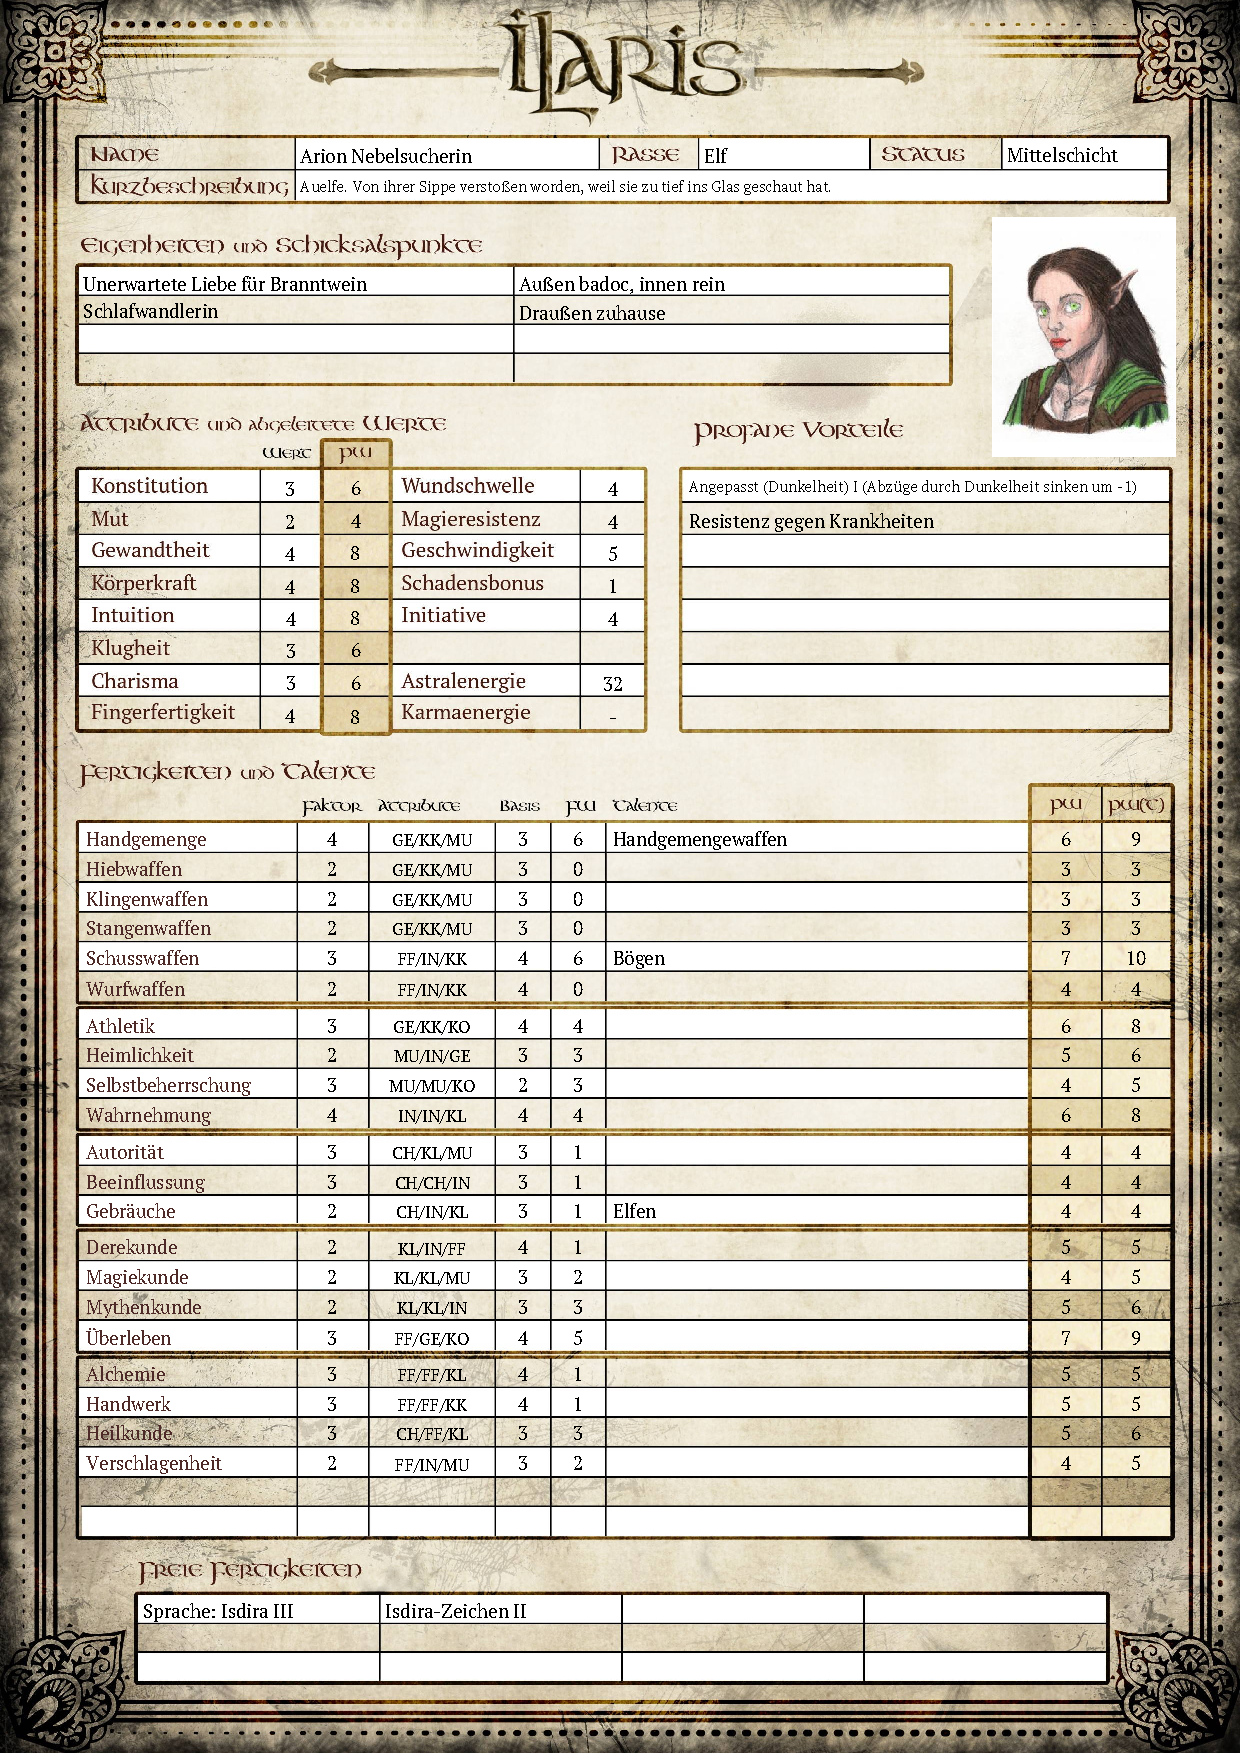
\includepdf[pages=-,addtotoc={1,subsection,1,Charakterbogen Arion Nebelsucherin,arion}]{klamm_und_heimlich/charaktere/arion_nebelsucherin.pdf}
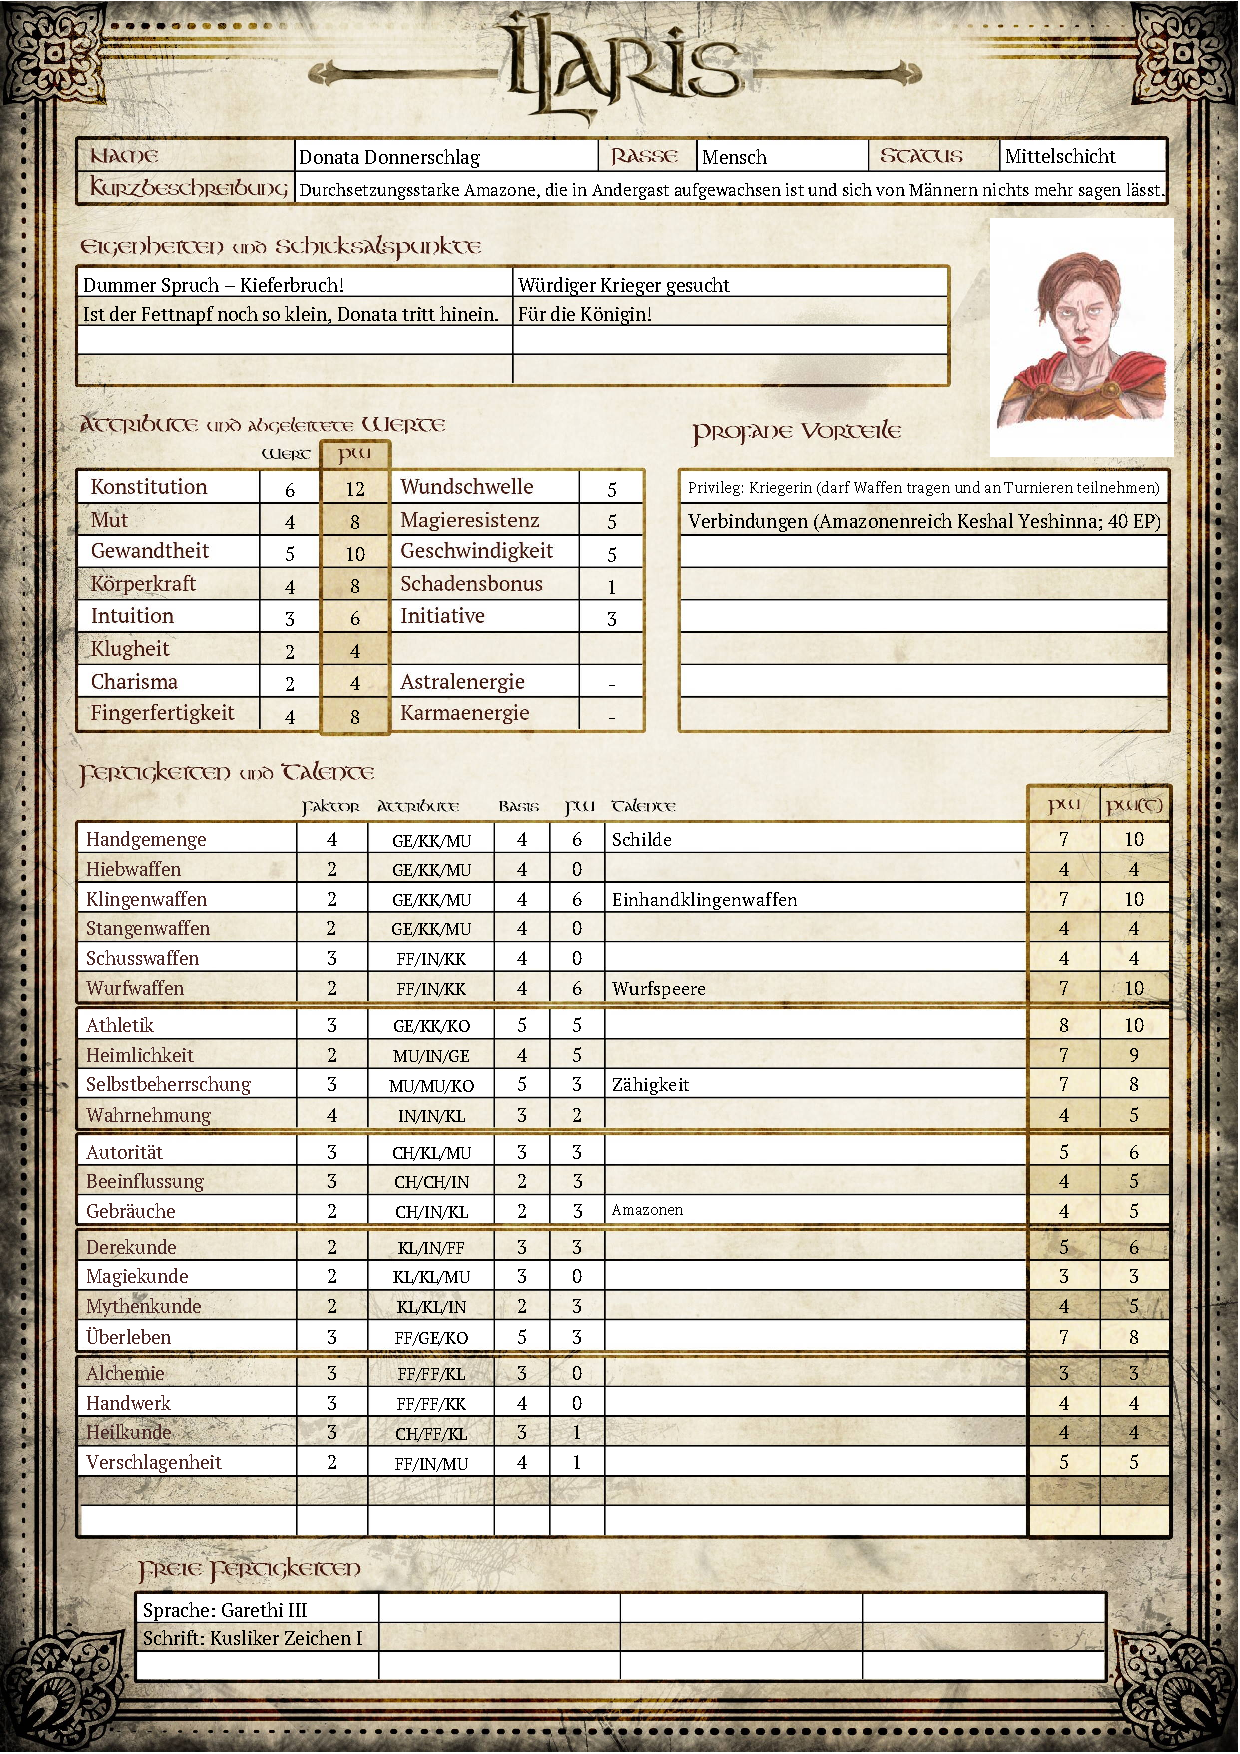
\includepdf[pages=-,addtotoc={1,subsection,1,Charakterbogen Donata Donnerschlag,donata}]{klamm_und_heimlich/charaktere/donata_donnerschlag.pdf}
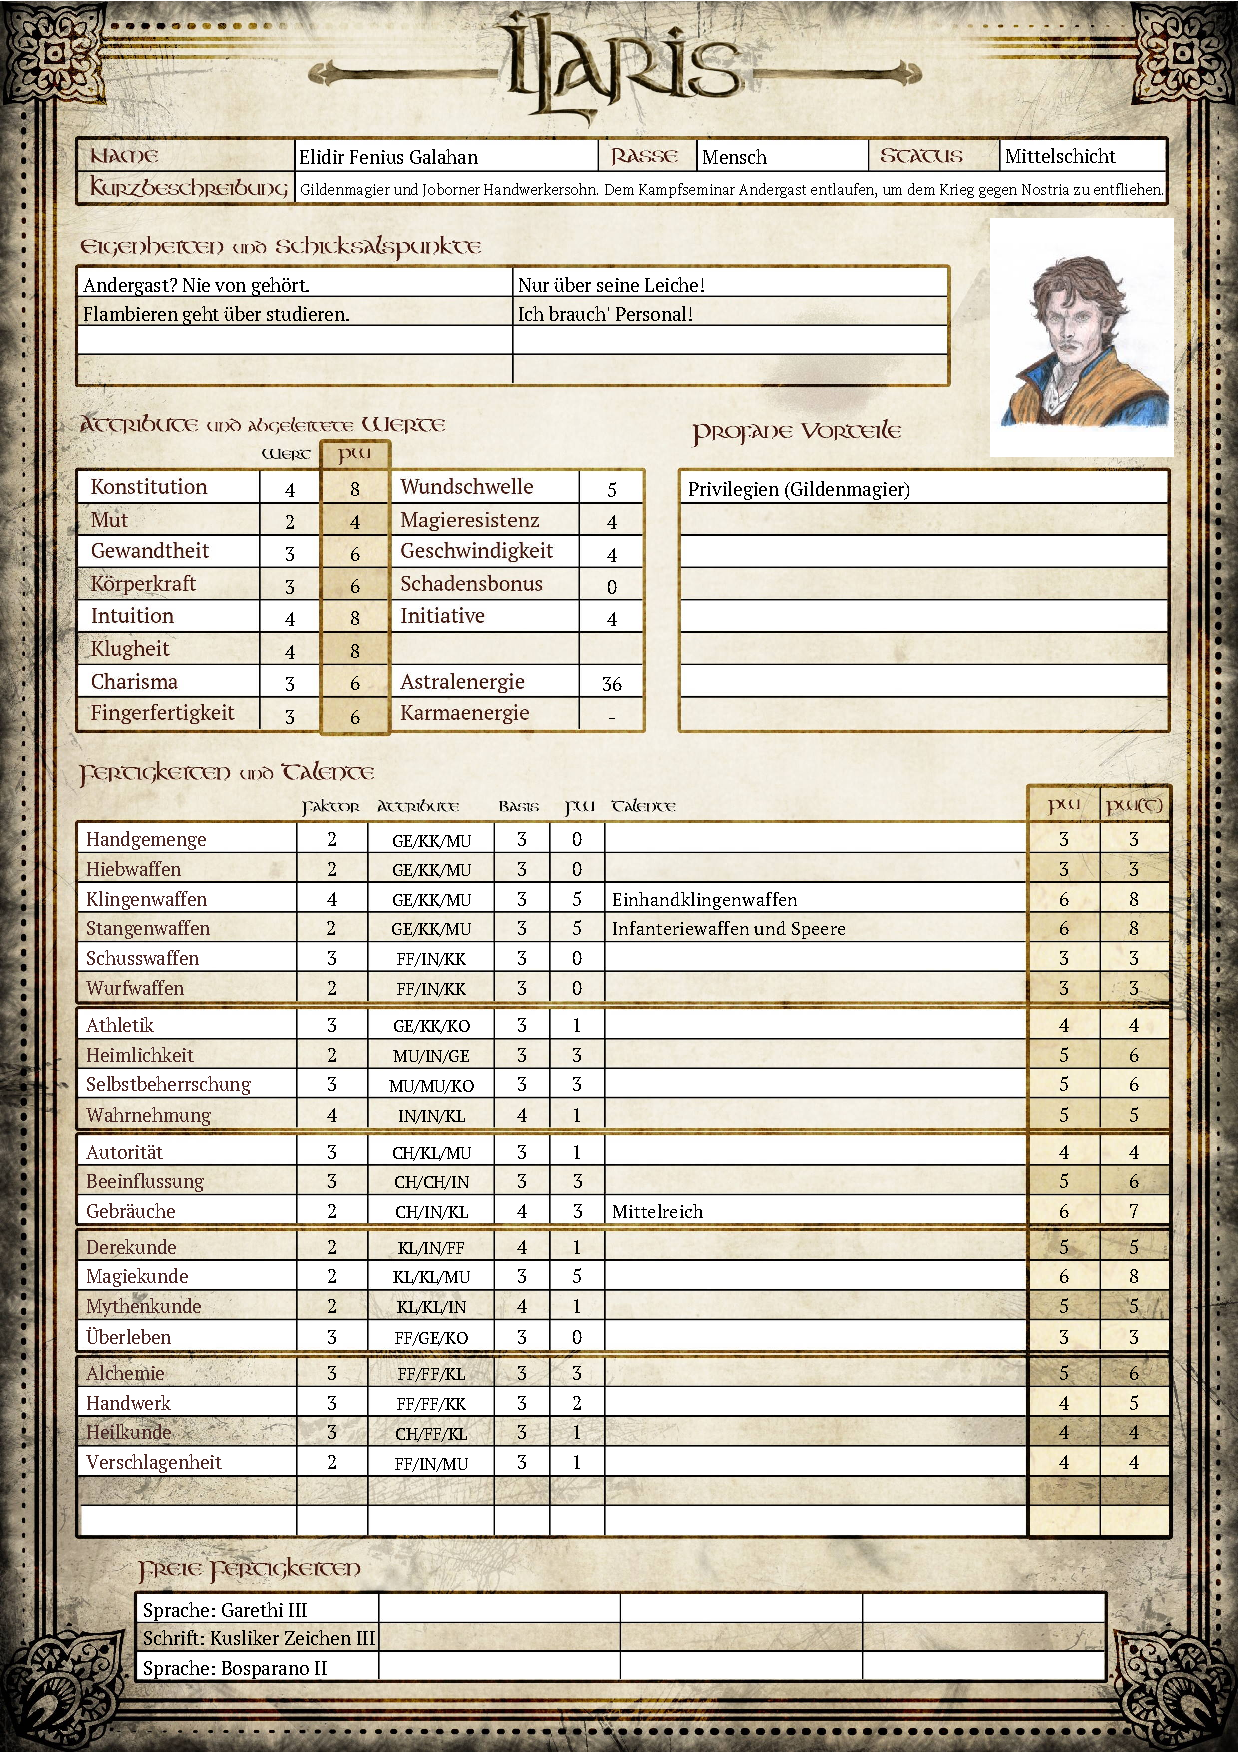
\includepdf[pages=-,addtotoc={1,subsection,1,Charakterbogen Elidir Fenius Galahan,elidir}]{klamm_und_heimlich/charaktere/elidir_fenius_galahan.pdf}
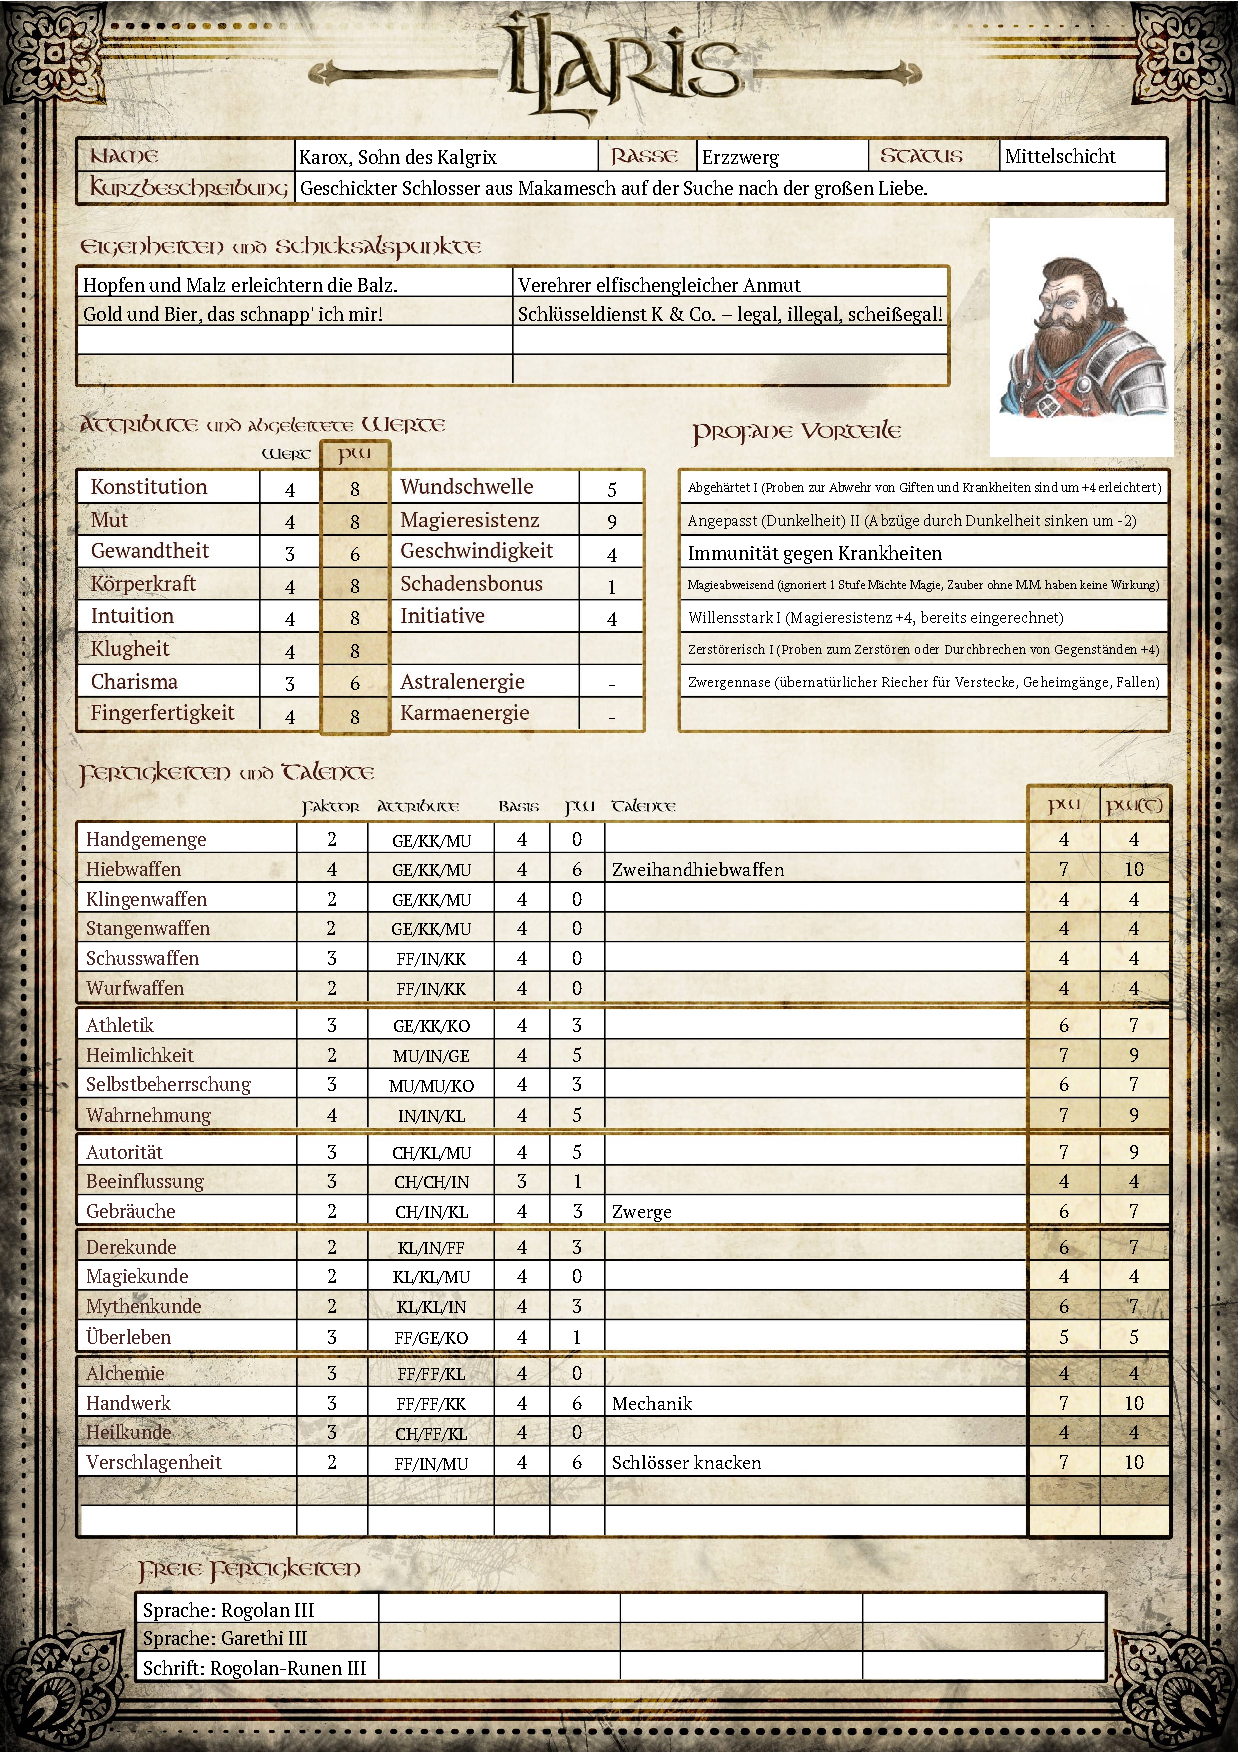
\includepdf[pages=-,addtotoc={1,subsection,1,Charakterbogen Karox Sohn des Kalgrix,karox}]{klamm_und_heimlich/charaktere/karox_sohn_des_kalgrix.pdf}
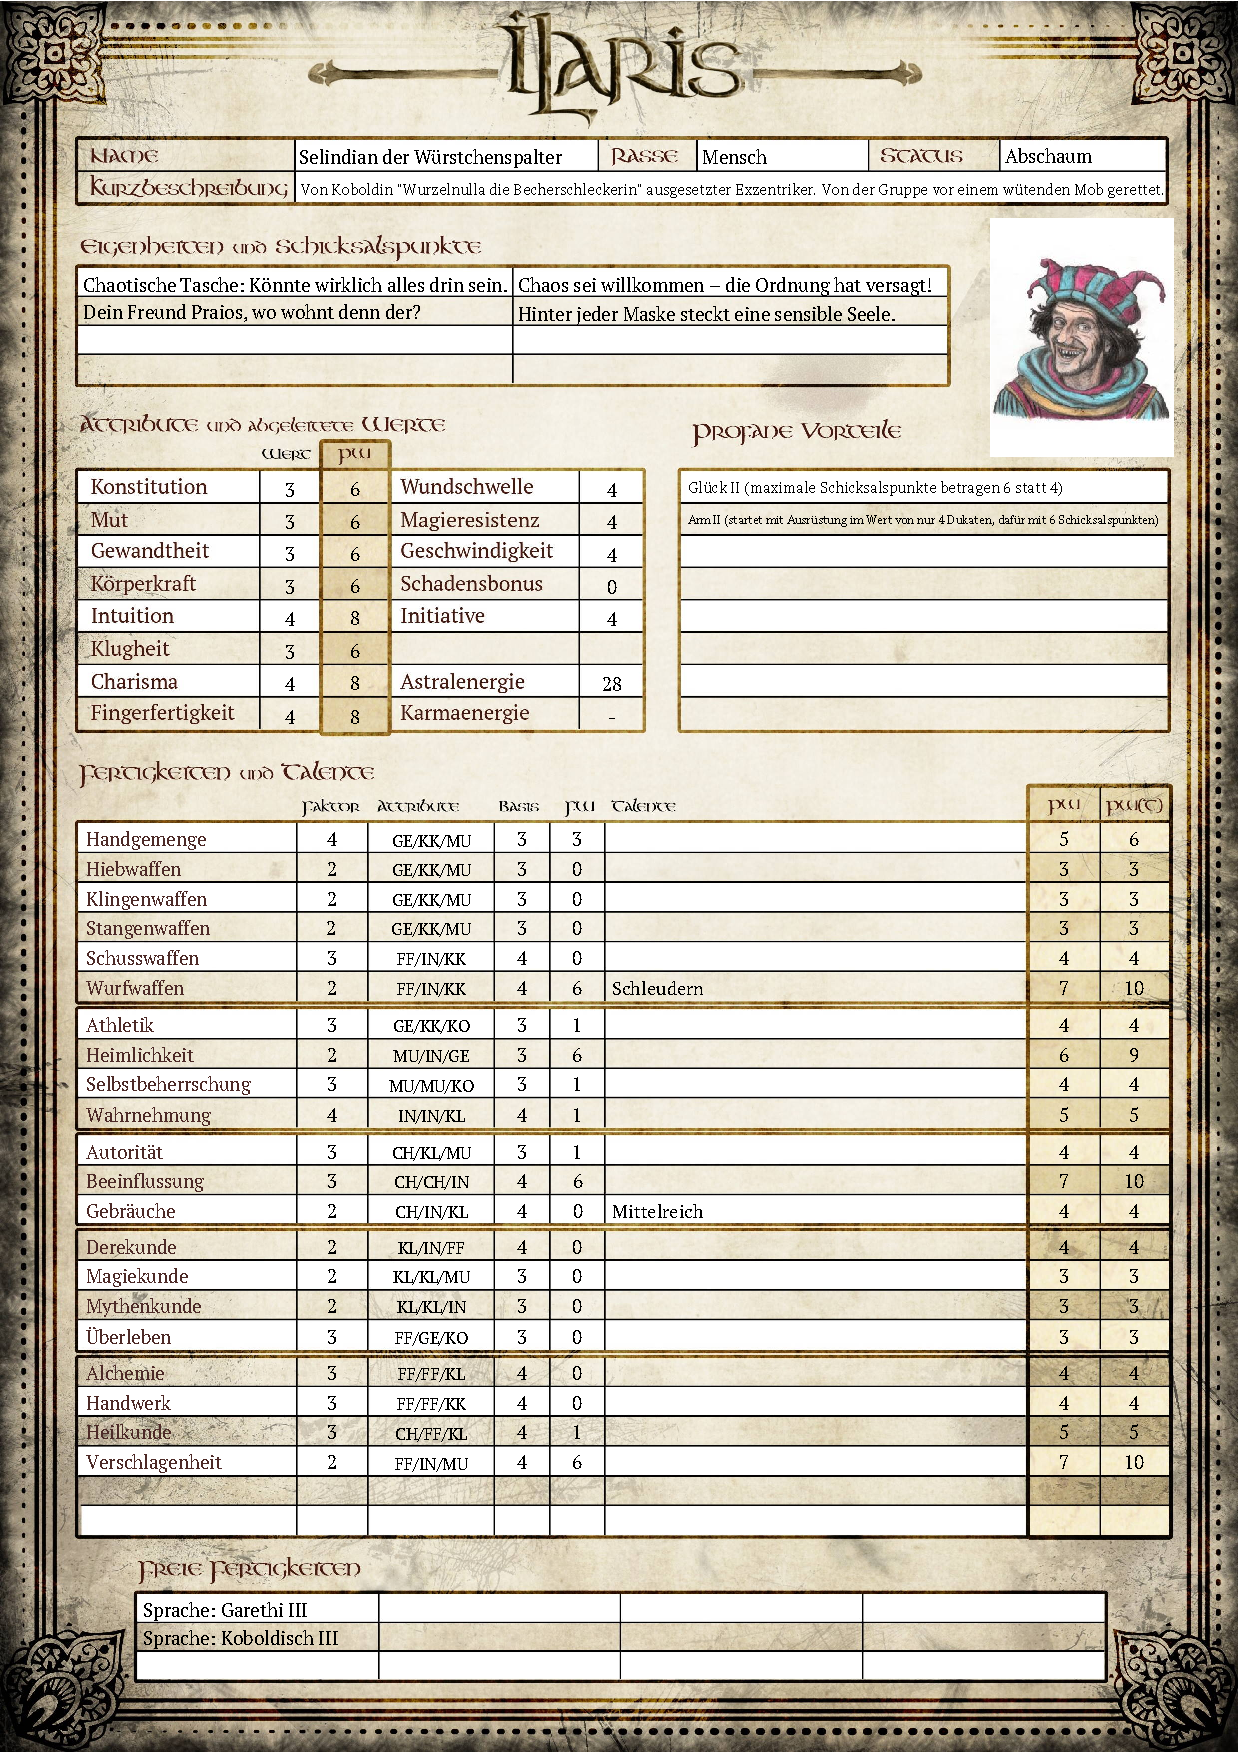
\includepdf[pages=-,addtotoc={1,subsection,1,Charakterbogen Selindian,selindian}]{klamm_und_heimlich/charaktere/selindian_der_wuerstchenspalter.pdf}

\section{Asche im Wind}
\absatz{Karte des Svelltlands}

Die von \textbf{telling} gemachte Karte des Svelltlandes findet sich in tellings Blog \href{https://tellingaventurien.home.blog/2023/02/27/karte-svelltland-um-1045-nach-bosparans-fall/}{\textbf{\enquote{Zwischen Tisch und Telling}}}.

Mit freundlicher Genehmigung des Autors:

\begin{center}
	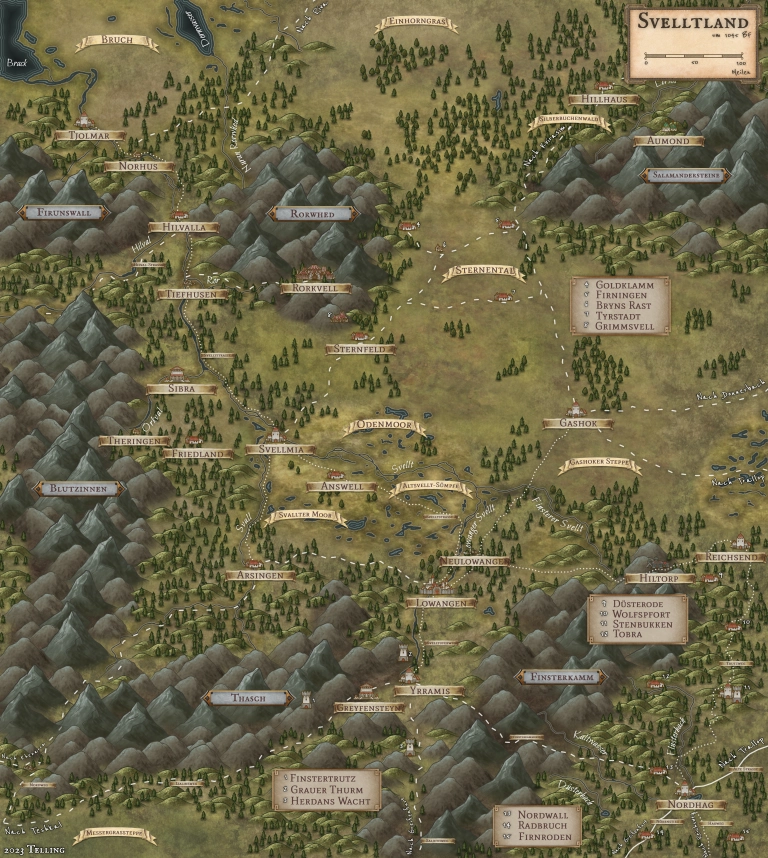
\includegraphics[width=\textwidth]{svellttal-0211.png}
\end{center}

\newpage

\kasten{
	\absatz{Quelle 1: Augenzeugenbericht}
	\label{aiw_quelle1}
	\enquote{Der Angriff hat nachts stattgefunden.
		Es schien plötzlich noch dunkler zu werden und ein Rauchgeruch hing in der Luft, der nicht von unserem kleinen Feuer stammen konnte.
		Beißender Qualm hat einen nach dem anderen zum Husten gebracht und die Sicht war schlecht. Die Gestalt, die dann aufgetaucht ist, schien geradewegs vom Himmel auf uns herabzufahren und aus Rauch und Qualm zu bestehen. Um sie herum begann das Gras zu schwelen und zu verkohlen. Wir leisteten kurz Widerstand, konnten aber gegen die allgegenwärtige Hitze nicht lange ankommen, zumal uns das Atmen schwer fiel. Inmitten des dichtesten Qualms habe ich aber eine etwa menschengroße Gestalt ausmachen können, die mich an ein Zündholz erinnert hat oder an eine halb erstickte Fackel, denn sie war dünn und verkohlt. Halb geblendet und nach Luft ringend sind alle in die Nacht geflohen, jeder in eine andere Richtung. Als ich an den Fluss kam, konnte ich mich dort im Dickicht am Ufer verbergen und mir den ganzen Ruß abwaschen. Noch am nächsten Morgen brannten mir die Augen.}
}

\absatz{Quelle 2: Die Weinlegende}
\label{aiw_quelle2}
Ihr betretet eine Holzhütte, die aussieht, als wäre sie vor kurzem aus frischen Buchenholz zusammengeschustert worden und die euch als Gasthaus beschrieben wurde. Innendrin entdeckt ihr einen schummrigen Saal mit vielen langen Tafeln und ihr seid erleichtert, dass der Duft des frischen Holzes noch nicht von diversen anderen Gerüchen jahrelangen Tavernenbetriebes überlagert wird.

Nur die bunt zusammengewürfelte Gruppe von Berufs- und Hobbytrinkern stört das würzige Aroma des hellen Schankraumes.
Diese hat sich in der Nähe des Tresens um einen älteren Gesellen mit roter Nase versammelt, dem gerade ein neues Glas Schnaps eingeschenkt wird.

\enquote{Wo war ich?}, stammelt der Alte.\\
\enquote{Bei Jokmanns Wein, Opa}, erklärt einer der Männer ungeduldig.\\
\enquote{Ach ja. Also das war damals so: Wie ich schon sagte, hatte der alte Jokmann das Jagen schon halb aufgegeben, weil das Revier, das er damals vom alten Firnwulf geerbt hatte, von dem alten Gierschlund so richtig ratzekahl leergejagt worden ist. Da hattest du vielleicht höchstens eine einzige Wildschweinrotte mit 10 Tieren, die Hälfte davon waren Frischlinge, alle noch an Mutterns Zitze und die andere Hälfte war so alt und zäh, die hätte nicht mal unser guter Alrik hier weichgeschmort bekommen.\\	
	Der Rest vom Wild hatte sich komplett drüben zu den Hexen verdrückt, weil die nix dagegen hatten, dass die die ganzen Jungtriebe von den Tannen abknabbern. Aber wenn du die das machen lässt, dann hast du ruckzuck den ganzen Wald kaputt und dann ist gar nix mehr mit jagen, das sag ich dir!
	
	Na ja, wie ich sagte, Jokmann war ziemlich am Ende. Und dann sagte er sich:
	\enquote{Komm, einen letzten Ausflug machst du noch und wenn Firun dann nicht mit dir ist, dann gehst du zurück in die Stadt und suchst dir eine Anstellung bei einem Bogenbauer oder beim Jagdvogt oder so.}
	Also schnappt er sich seinen treuen Hund Pix und marschiert in die Wildnis. Wir dachten damals ja, den sehen wir nie wieder, ich mein, wir waren damals ja auch nur kleine Stöpsel und der hatte so einen grimmigen Gesichtsausdruck. Und dann kam eine Woche später auch noch ein Sturm auf und keine Spur von Jokmann! Aber als wir schon alle Hoffnung aufgeben wollten, stapft der plötzlich in einer Vollmondnacht in den alten Gasthof und ihr glaubt nicht, wie der aussah! Nix mit dem schmucken Ledermantel, den er anhatte, als er losging, nein! Einen Wildschweinpelz trug er, mit so farbigen Verzierungen drauf und der roch! Der halbe Schankraum hat ihn angestarrt, als wäre er aus Borons Hallen selbst entwischt, gesegnet sei der Rabe.}

Ihr merkt wie die Spannung unter den Zuhörern steigt. Lange kann es nicht mehr dauern, bis die Geschichte ihrem Höhepunkt zustrebt.\\
\enquote{Na ja, dann waren natürlich alle erst mal heilfroh, dass Jokmann noch da war, vor allem, als man gemerkt hat, dass da immer noch der alte Halunke unter dem Pelz steckt. Den Hund hat er auch wieder mitgebracht und der sah auch aus, als hätte den jemand angemalt. Komisch wurde die Sache aber erst in den Wochen danach. Der ist nämlich dann nicht in die Stadt gegangen für eine Anstellung, nein, der ist im Jagdrevier vom alten Firnwulf geblieben. Der hat sogar die anderen zu einer Drückjagd eingeladen, weil er da den prächtigsten Hirsch gesehen haben wollte, den Tsa jemals auf Dere geschickt haben soll. Die einzige Bedingung war, dass sie alle vorher mit ihm diesen Wein trinken mussten, sonst würde die Jagd schiefgehen.}

Ihr könnt schwören, Opas Zuhörer halten den Atem an. Einer hüstelt kurz, worauf ihn alle anzischen.
\enquote{Das war ein seltsames Gesöff. Schmeckte fast wie Heidelbeerwein, aber irgendwie fad und erdig. Ich musste es einmal trinken, als sie mich bei einer Jagd als Treiber mitgenommen haben. Ist sofort in die Birne gestiegen und am Ende hab ich mein Mittagessen wieder ausgekotzt. Und die Flasche in der das war, ich will nicht wissen, wo die schon alles gewesen ist. Das war so eine raue Tonkaraffe mit ganz seltsamen Bildchen drauf, so Schweine und kleine Männchen mit Speeren.
	
	Na ja, Jokmann hat halt alle dazu gedrängt, das Zeug zu trinken und los. Und tatsächlich sind die nach sieben Stunden mit einer fetten Hirschkuh als Beute zurückgekommen und die Leute haben noch Tage danach davon geschwärmt, dass der Hirsch, der die Kühe begleitet habe, der größte gewesen sei, den sie je gesehen hätten. Der bekam mit jedem Mal erzählen mehr Enden an seinem Geweih, ich sag's euch! 
	
	Ja, und seitdem hatte der alte Jokmann nie wieder Pech beim Jagen, so lange er diesen Wein hatte. Und jedes mal, wenn wir dachten, die Flasche muss doch jetzt mal leer sein, ist der wieder für eine Woche im Wald verschwunden und dann war die wieder voll. Und bis zu seinem Todestag hat er dicht gehalten, wo er diesen Wein her hatte! Obwohl sich alle die Mäuler darüber zerrissen haben, mit Feenhügeln und Dämonenpakten und sonst noch was. Nie hat der was durchschlüpfen lassen! So, das ist jetzt die ganze Geschichte, jetzt gib mir mal was zu trinken, meine Kehle ist ja schon ganz trocken!}

Nachdem das Glas eilig aufgefüllt wurde, breitete sich Gemurmel in der Schankstube aus.
\enquote{Ob diese wandernden Fässer im Wald mit Jokmanns legendärem Wein zu tun haben?}\\
\enquote{Irgendetwas muss es damit auf sich haben, warum sonst sollte die Torfkompagnie eine Belohnung auf die Fässer ausgerufen haben?}



\absatz{Eigenheiten der Archetypen}

\spaltenanfang

\kreatur{Alruna \enquote{Eisen-Ala}}{}{humanoid}{
	\kreaturinfo{Düstere Vergangenheit}{Einen Teil ihrer Kampfausbildung verdankt sie ihrer Jugend bei den Schwarzamazonen. Zwar hat sie diesen Zeiten längst den Rücken gekehrt, doch beherrscht sie noch einige schmutzige Tricks und Techniken, die nicht als sonderlich rondragefällig gelten können. In vielen Regionen muss sie ihre Vergangenheit geheim halten.}
	\trennlinie
	\kreaturinfo{Von Rang und Namen}{Als Kriegerin wird sie hochgeschätzt und sie hat gelernt, sich entsprechend zu verhalten. Doch ihr Kriegerbrief ist in Wahrheit eine Fälschung.}
}
\kreatur{Falkja}{}{humanoid}{
	\kreaturinfo{Im Dienste der Schwänin}{Sie hat ihr Leben Ifirn geweiht und befolgt ihre Gebote.}
	\trennlinie
	\kreaturinfo{Meine Heimat - die Weite}{Sie hat den Großteil ihres Lebens in den Weiten des Nordens verbracht. Große Städte sind ihr schnell zu eng und mit Kälte kann sie besser umgehen als mit Hitze.}
	\trennlinie
	\kreaturinfo{Brückenbauen}{Sie strebt danach, Brücken zwischen den Elfen und den Zwölfgötter-Anhängern zu schlagen, die oft getrennte Gemeinschaften sind.}
}
\kreatur{Melcher}{}{humanoid}{
	\kreaturinfo{Kein Ekel, aber ekelig}{Er hat keine Scheu, sich alles anzusehen oder etwas anzufassen -- kommt gut mit Schmutz klar,  das merkt man ihm auch oft später noch an.}
	\trennlinie
	\kreaturinfo{Tiere sind die besseren Menschen}{Er kommt einfach besser mit Tieren aus.}
	\trennlinie
	\kreaturinfo{Netter Kauz}{Man traut ihm zu, über manche speziellen Themen Bescheid zu wissen -- aber sicher nicht über alles. Ein sympathischer Typ, aber ein bisschen verrückt.}
}

\kreatur{Roana}{}{humanoid}{
	\kreaturinfo{Nebulöser Charakter}{Sie wirkt mysteriös und manchmal unauffällig, aber auch nicht immer sonderlich vertrauenswürdig -- besonders auf abergläubische Leute.}
	\trennlinie
	\kreaturinfo{Vergisst nie ein Gesicht}{Sie erkennt Leute immer wieder, doch ist dabei auch nachtragend und rachsüchtig.}
	\trennlinie
	\kreaturinfo{Wirren des Geistes}{Sie ist manchmal etwas verwirrt \dots in diesem Zustand kann sie leichter mit Geistern in Kontakt treten. Das mag zwar helfen, um diese zu bannen, führt aber manchmal im Gegenteil dazu, dass sie umso leichter einer Besessenheit erliegt.}
}

\kreatur{Wiesel-Rupo}{}{humanoid}{
	\kreaturinfo{Kennt keine Furcht\dots und keine Vernunft}{Er nimmt nichts wirklich ernst und alles auf die leichte Schulter und schätzt deshalb Risiken kaum ab. Die Leute
		bewundern seinen Mut, aber viele seiner Aktionen sind auch
		einfach leichtsinnig.}
	\trennlinie
	\kreaturinfo{Da gibt es doch ein Mittelchen}{Der Glaube des Charakters an die Wunder der Medizin ist stark ausgeprägt. Er hat selbst von eigentlich schlechten oder gar völlig unwirksamen Mitteln einen Placebo-Effekt, doch wird dementsprechend beim Angebot jedes Quacksalbers schwach.}
	\trennlinie
	\kreaturinfo{Die Wahrheit wäre auch zu langweilig}{Er neigt zu Übertreibungen und schindet damit bei einigen ordentlich Eindruck, bei anderen eher das Gegenteil.}
	\trennlinie
	\kreaturinfo{Die kriegen mich eh nie}{Er muss geradezu zwanghaft am Tatort sein Markenzeichen zurücklassen -- ein kleines Papier mit Schlangensymbol in die leere Hosentasche stecken oder in der leeren Schatztruhe platzieren. Das gibt ihm einfach diesen besonderen 		Adrenalinschub.}
}

\spaltenende


\neueseite
\ohnehintergrund
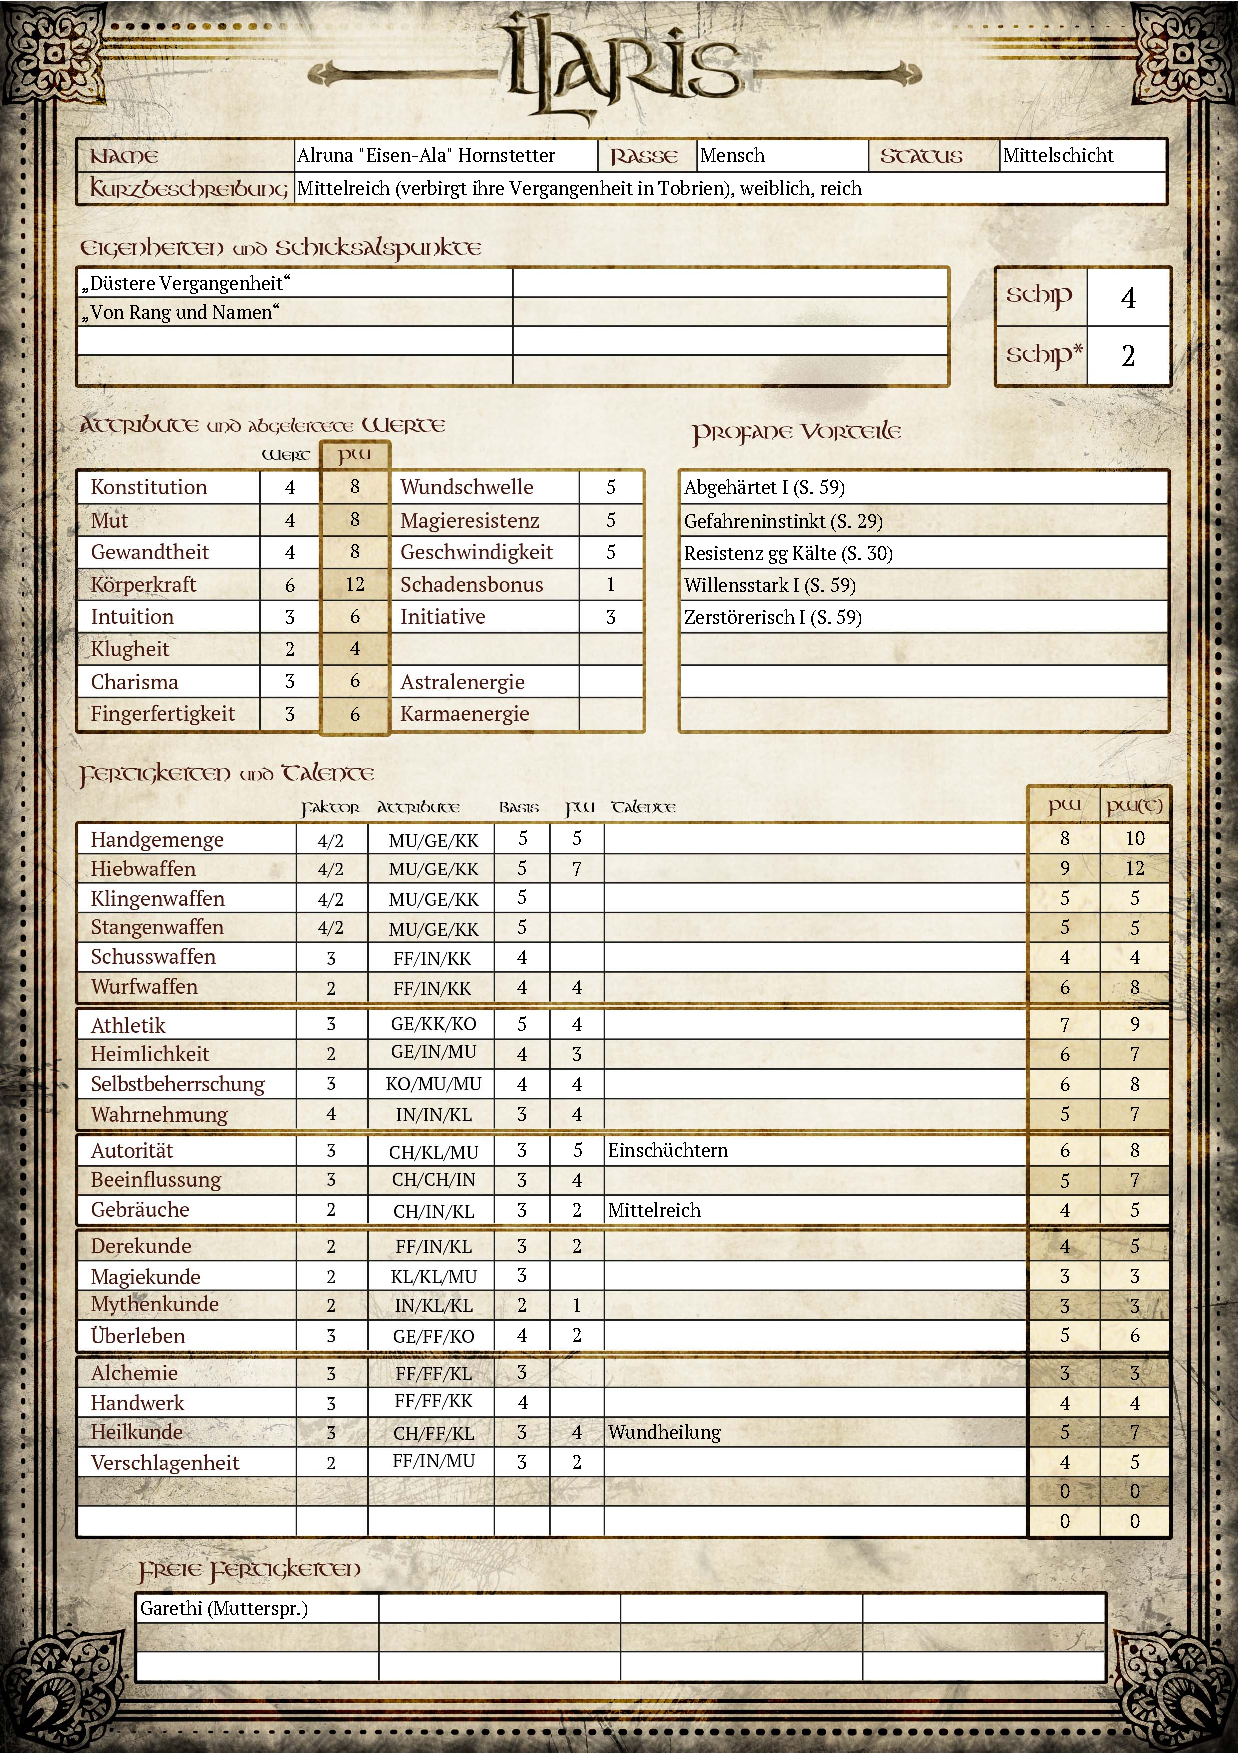
\includepdf[pages=1-2,addtotoc={1,subsection,1,Charakterbogen Alruna \enquote{Eisen-Ala},eisenala}]{asche_im_wind/charaktere/eisen_ala.pdf}
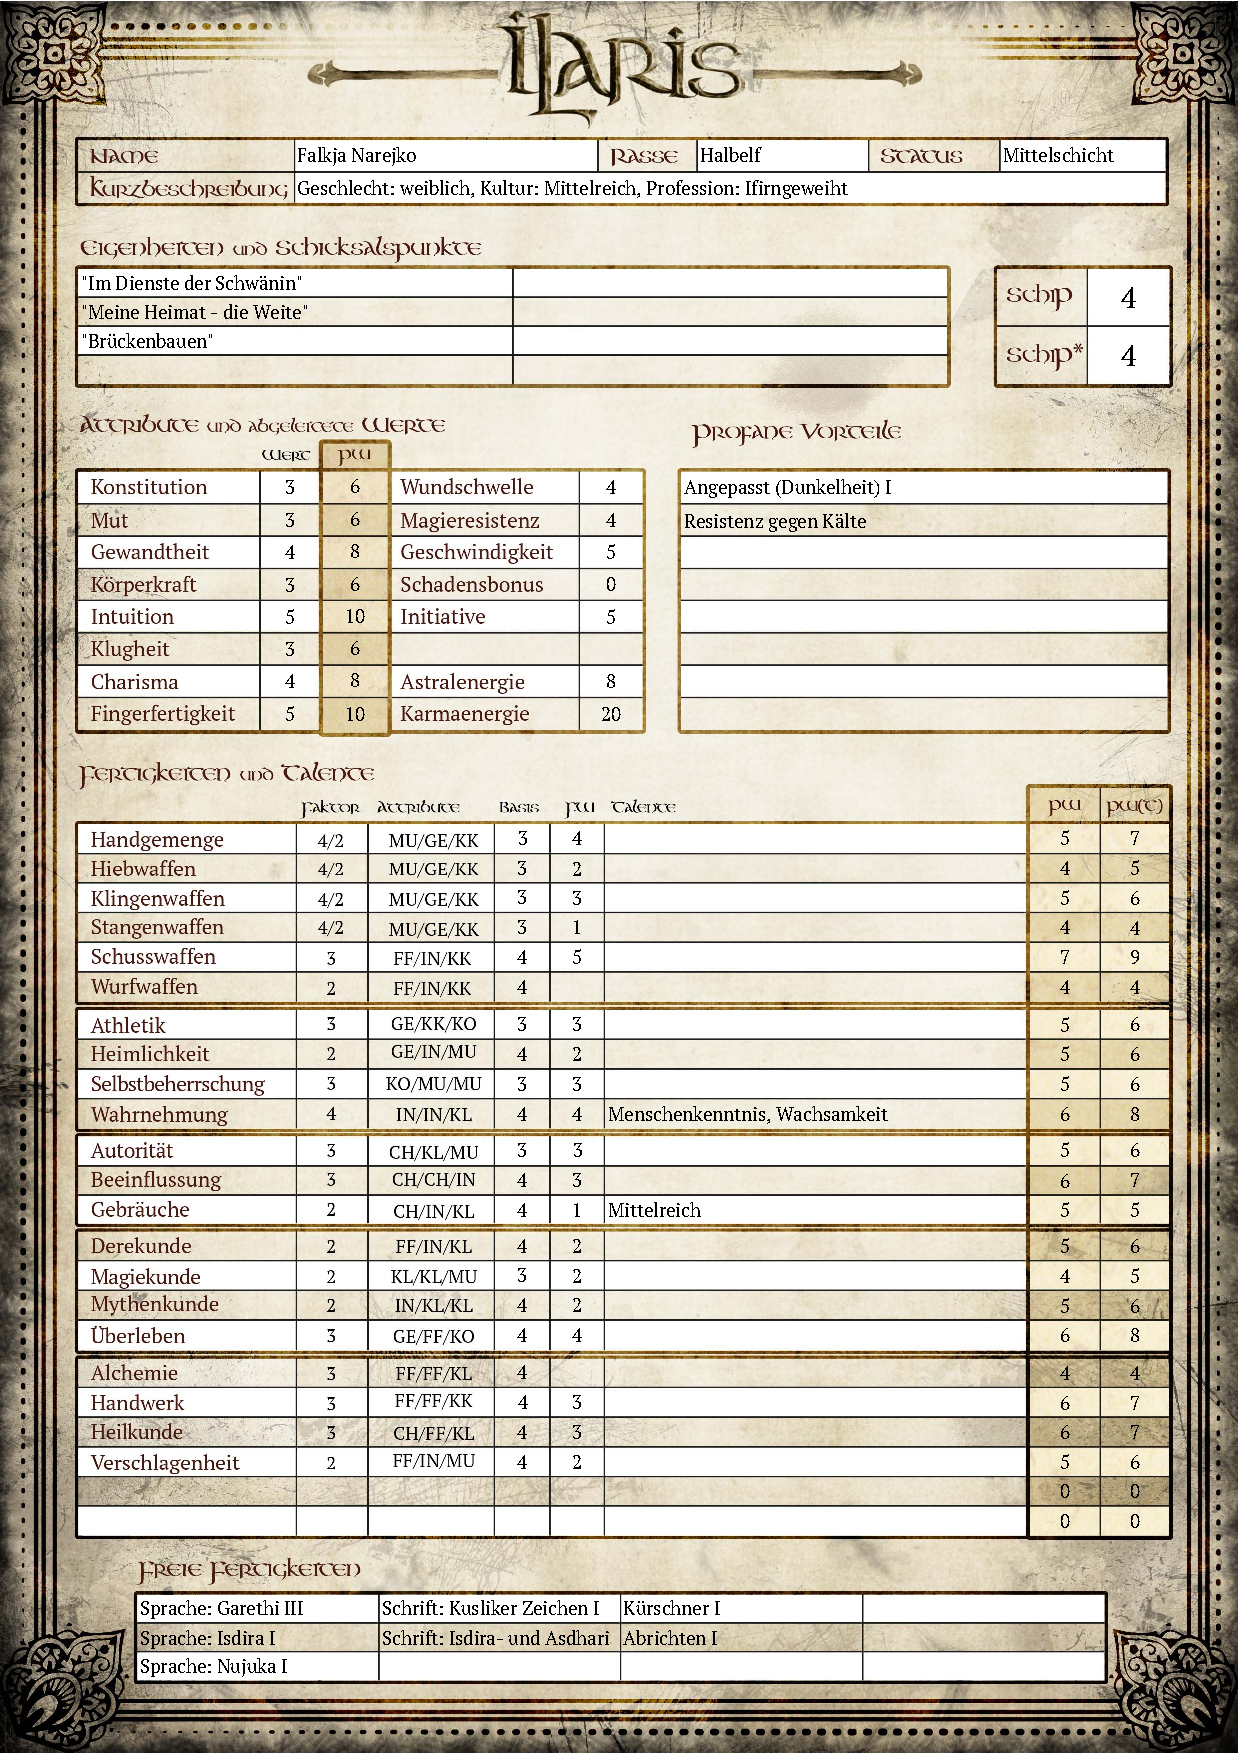
\includepdf[pages=-,addtotoc={1,subsection,1,Charakterbogen Falkja Narejko,falkja}]{asche_im_wind/charaktere/falkja_narejko.pdf}
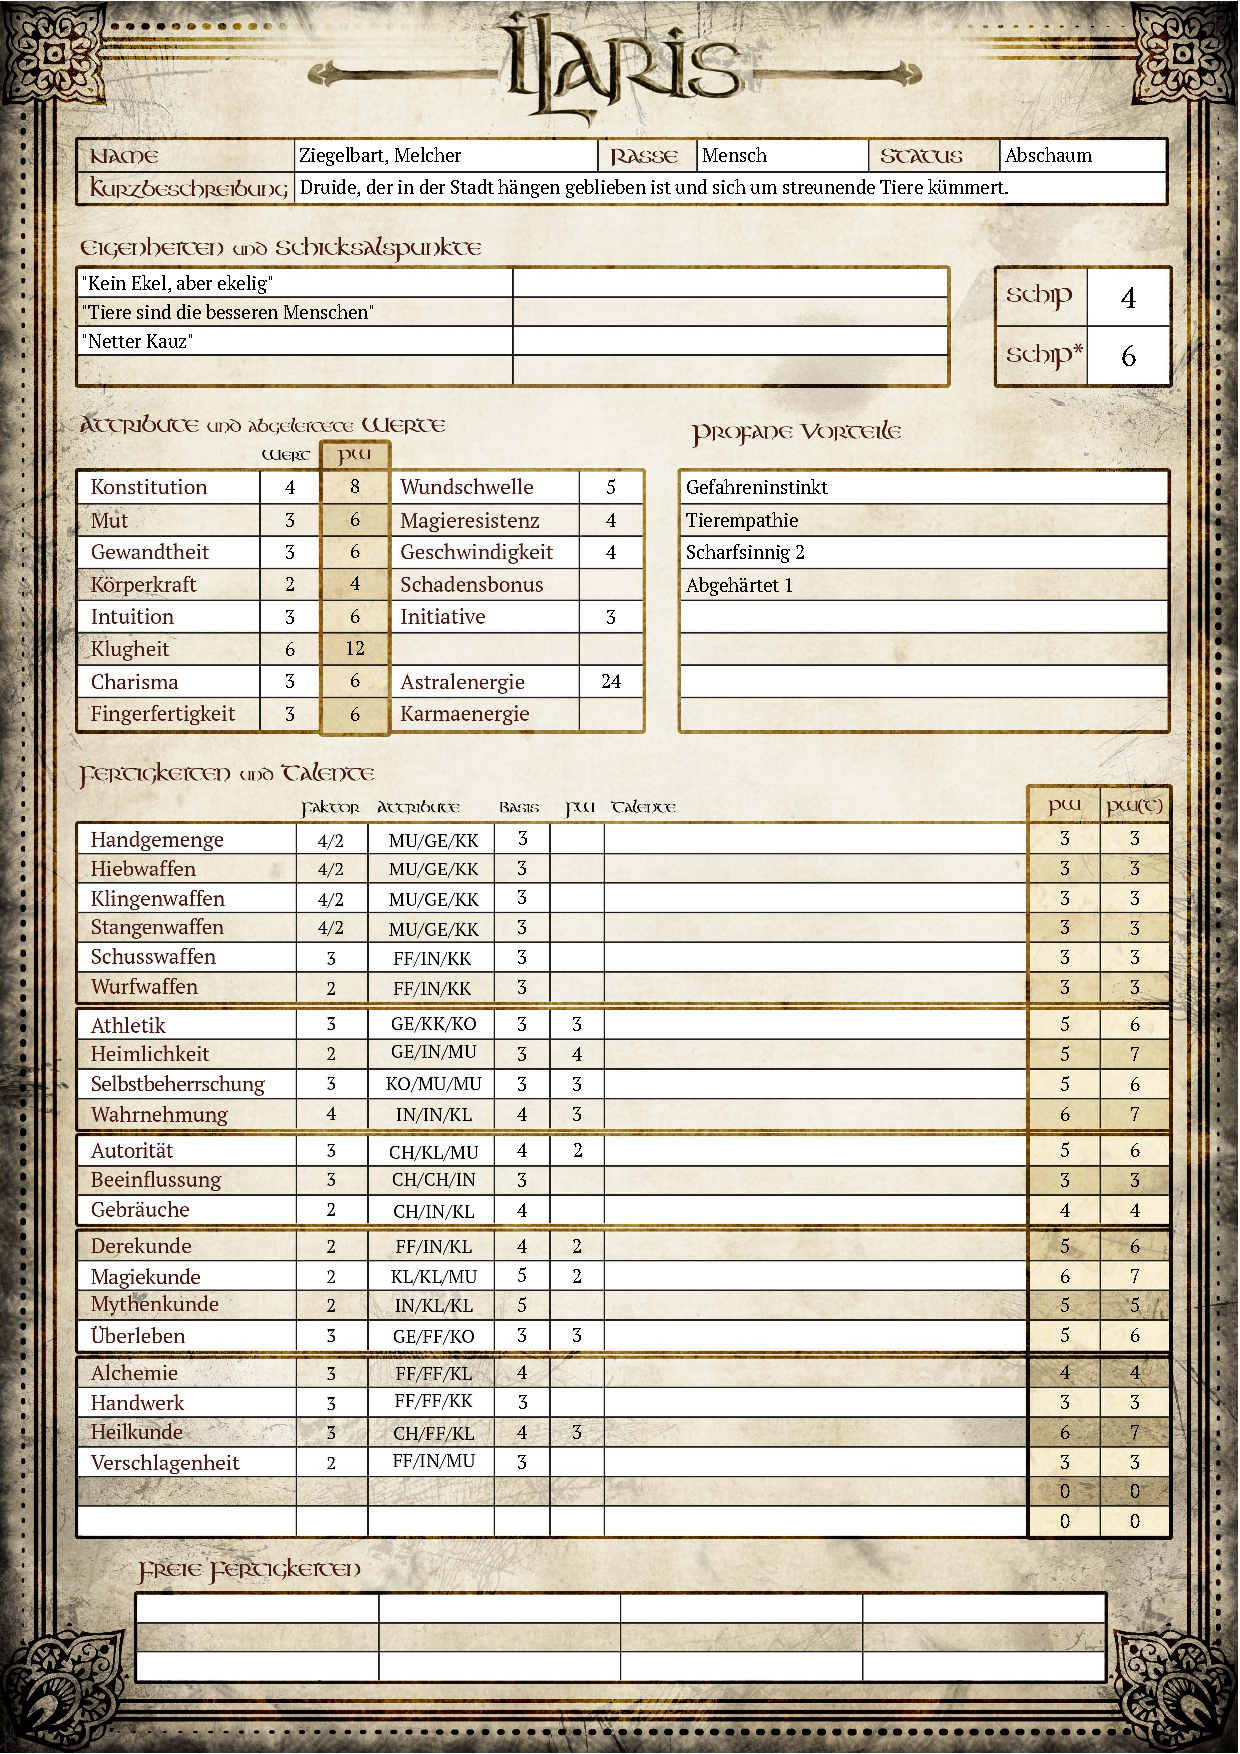
\includepdf[pages=-,addtotoc={1,subsection,1,Charakterbogen Melcher Ziegelbart,melcher}]{asche_im_wind/charaktere/melcher.pdf}
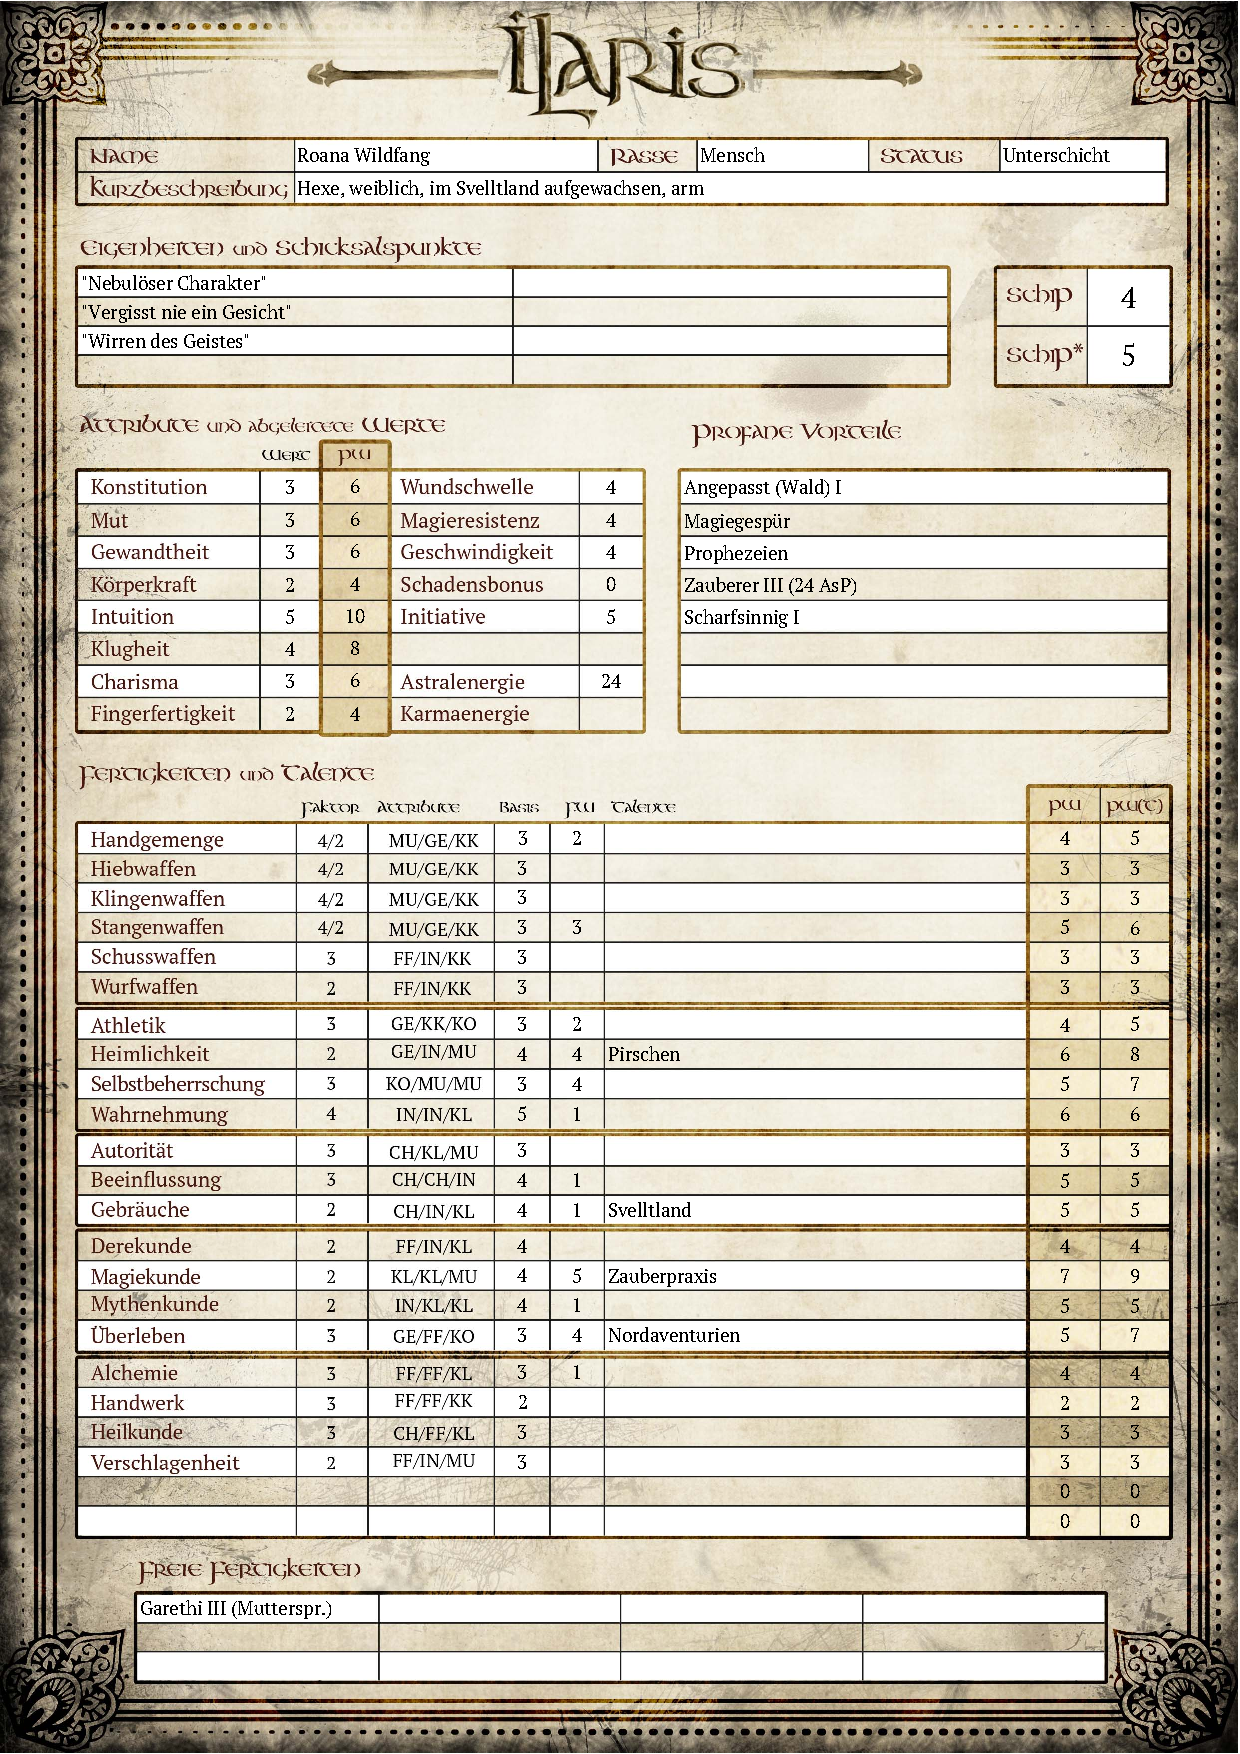
\includepdf[pages=-, addtotoc={1,subsection,1,Charakterbogen Roana Wildfang,roana}]{asche_im_wind/charaktere/roana_wildfang.pdf}
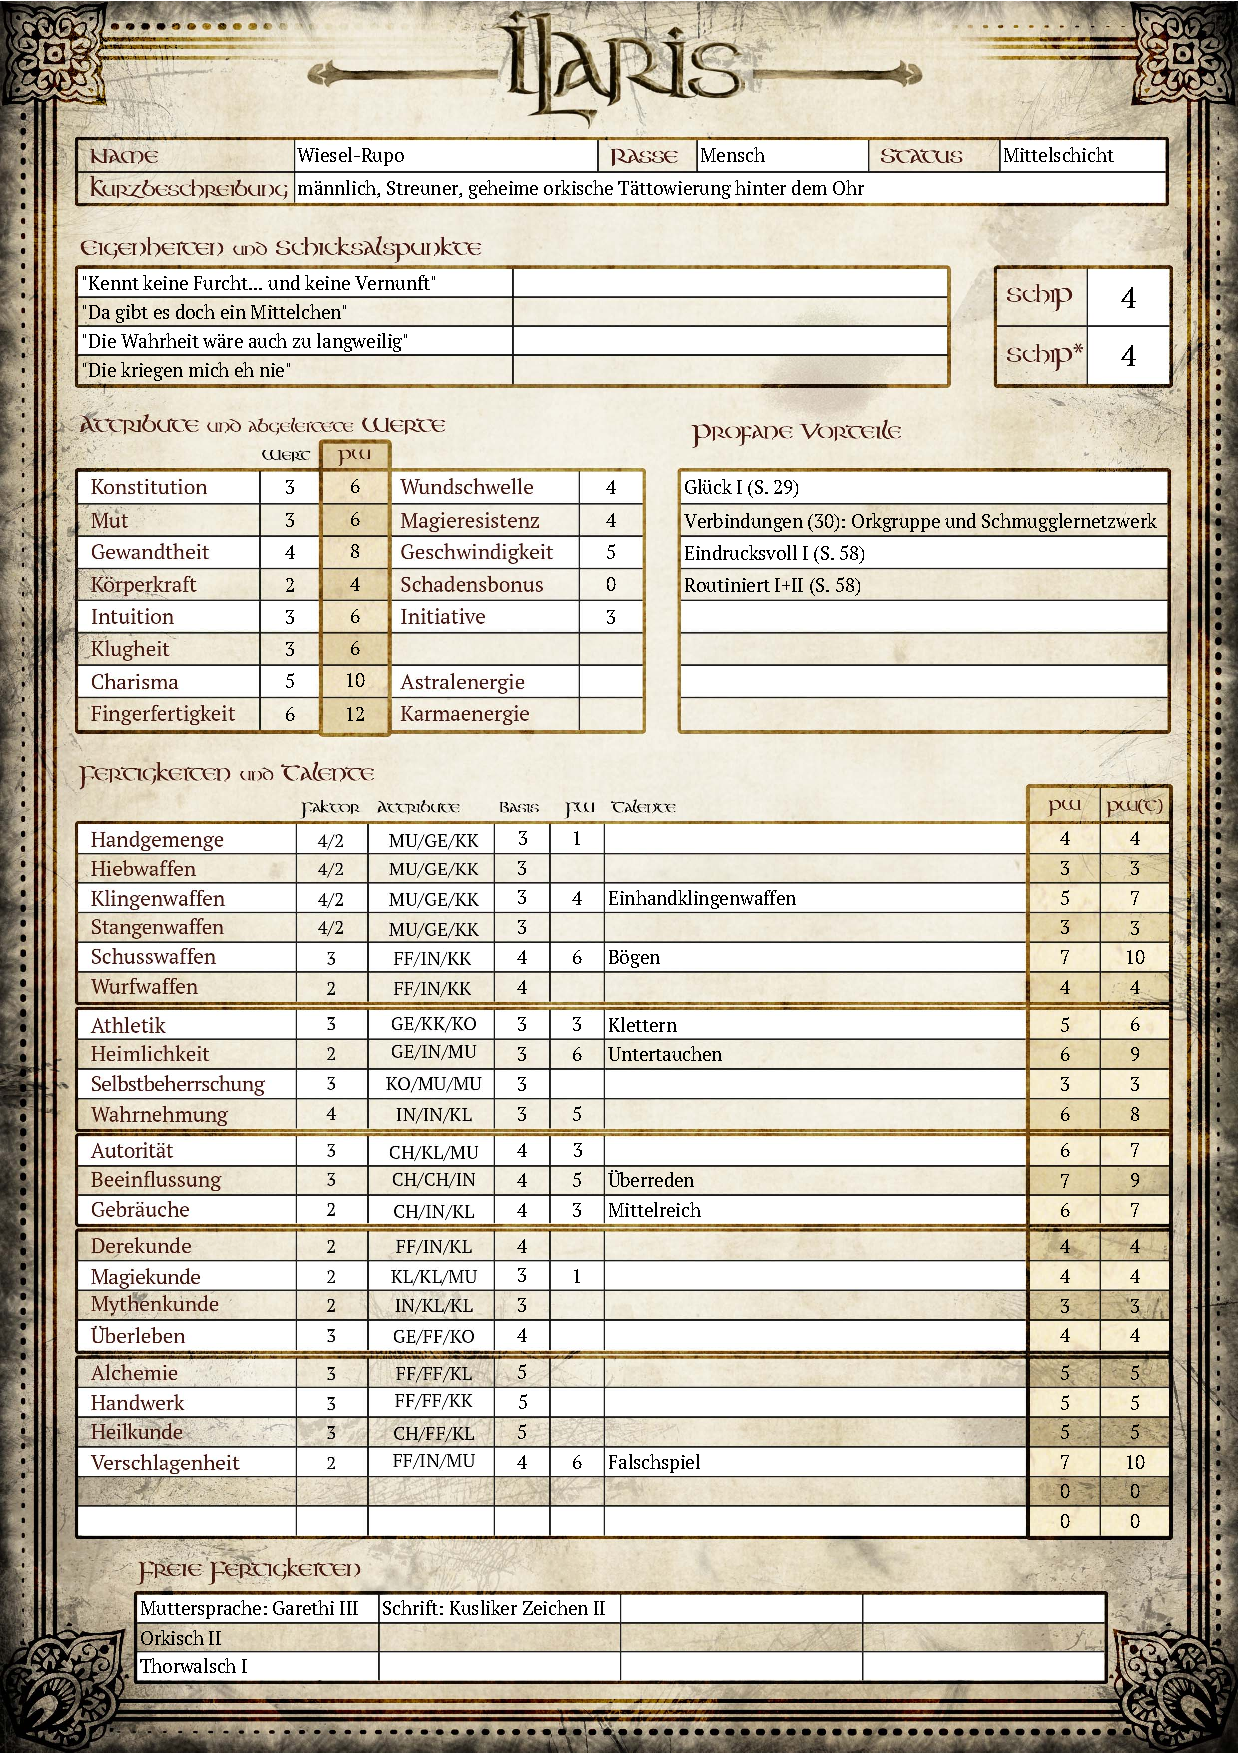
\includepdf[pages=1-2,addtotoc={1,subsection,1,Charakterbogen Wiesel-Rupo,rupo}]{asche_im_wind/charaktere/wiesel_rupo.pdf}
\neueseite
\handout
\section{In den Hallen des Bergkönigs}
\subsection{Das Relief hinter dem Angrosch-Altar}
%Lösung: D G M
\label{karten}
\mbox{}

\begin{center}
	\bigskip
	\vfill
	
\includegraphics[width=0.5\textwidth]{ngrsch.png}
\end{center}

\vfill

\begin{multicols}{3}
	\karte{
		\begin{multicols}{3}\mbox{ }\linebreak \begin{tabularx}{1.5cm}{|X|}
				\leer \leer \amboss \amboss
				\hline	\end{tabularx}	\neuespalte
			\begin{center} \mbox{ } \linebreak[4]
				
\includegraphics[width=\columnwidth]{S.png}
			\end{center} \neuespalte \mbox{ } \begin{tabularx}{1.5cm}{|X|}
				\amboss \leer \leer \leer
				\hline \end{tabularx} \end{multicols}
	}\vfill
	
	\karte{
		\begin{multicols}{3}\mbox{ }\linebreak \begin{tabularx}{1.5cm}{|X|}
				\amboss \leer \amboss \leer
				\hline	\end{tabularx}	\neuespalte
			\begin{center} \mbox{ } \linebreak[4]
				
\includegraphics[width=\columnwidth]{B.png}
			\end{center} \neuespalte \mbox{ } \begin{tabularx}{1.5cm}{|X|}
				\leer \amboss \leer \amboss
				\hline \end{tabularx} \end{multicols}
	}\bigskip
	
	\karte{
		\begin{multicols}{3}\mbox{ }\linebreak \begin{tabularx}{1.5cm}{|X|}
				\amboss \leer \leer \amboss
				\hline	\end{tabularx}	\neuespalte
			\begin{center} \mbox{ } \linebreak[4]
				
\includegraphics[width=\columnwidth]{G.png}
			\end{center} \neuespalte \mbox{ } \begin{tabularx}{1.5cm}{|X|}
				\leer \amboss \amboss \leer
				\hline \end{tabularx} \end{multicols}
	}\bigskip
	
	
	\karte{
		\begin{multicols}{3}\mbox{ }\linebreak \begin{tabularx}{1.5cm}{|X|}
				\amboss  \amboss \leer \leer
				\hline	\end{tabularx}	\neuespalte
			\begin{center} \mbox{ } \linebreak[4]
				
\includegraphics[width=\columnwidth]{N.png}
			\end{center} \neuespalte \mbox{ } \begin{tabularx}{1.5cm}{|X|}
				\leer  \leer \leer \leer
				\hline \end{tabularx} \end{multicols}
	}\bigskip
	
	\karte{
		\begin{multicols}{3}\mbox{ }\linebreak \begin{tabularx}{1.5cm}{|X|}
				\leer \leer \leer \amboss
				\hline	\end{tabularx}	\neuespalte
			\begin{center} \mbox{ } \linebreak[4]
				
\includegraphics[width=\columnwidth]{F.png}
			\end{center} \neuespalte \mbox{ } \begin{tabularx}{1.5cm}{|X|}
				\amboss  \amboss \amboss \leer 
				\hline \end{tabularx} \end{multicols}
	}\bigskip
	
	\karte{
		\begin{multicols}{3}\mbox{ }\linebreak \begin{tabularx}{1.5cm}{|X|}
				\leer \amboss \amboss \amboss
				\hline	\end{tabularx}	\neuespalte
			\begin{center} \mbox{ } \linebreak[4]
				
\includegraphics[width=\columnwidth]{J.png}
			\end{center} \neuespalte \mbox{ } \begin{tabularx}{1.5cm}{|X|}
				\amboss \leer \leer \leer
				\hline \end{tabularx} \end{multicols}
	}\bigskip
	
	
	\karte{
		\begin{multicols}{3}\mbox{ }\linebreak \begin{tabularx}{1.5cm}{|X|}
				\leer \leer \leer  \amboss
				\hline	\end{tabularx}	\neuespalte
			\begin{center} \mbox{ } \linebreak[4]
				
\includegraphics[width=\columnwidth]{H.png}
			\end{center} \neuespalte \mbox{ } \begin{tabularx}{1.5cm}{|X|}
				\amboss \amboss \leer \leer
				\hline \end{tabularx} \end{multicols}
	}\bigskip
	
	\karte{
		\begin{multicols}{3}\mbox{ }\linebreak \begin{tabularx}{1.5cm}{|X|}
				\leer \amboss \amboss \leer
				\hline	\end{tabularx}	\neuespalte
			\begin{center} \mbox{ } \linebreak[4]
				
\includegraphics[width=\columnwidth]{P.png}
			\end{center} \neuespalte \mbox{ } \begin{tabularx}{1.5cm}{|X|}
				\amboss \leer \leer \leer
				\hline \end{tabularx} \end{multicols}
	}\bigskip
	
	\karte{
		\begin{multicols}{3}\mbox{ }\linebreak \begin{tabularx}{1.5cm}{|X|}
				\leer \leer \leer \leer
				\hline	\end{tabularx}	\neuespalte
			\begin{center} \mbox{ } \linebreak[4]
				
\includegraphics[width=\columnwidth]{D.png}
			\end{center} \neuespalte \mbox{ } \begin{tabularx}{1.5cm}{|X|}
				\amboss \leer \amboss \amboss
				\hline \end{tabularx} \end{multicols}
	}\bigskip
	
	
	\karte{
		\begin{multicols}{3}\mbox{ }\linebreak \begin{tabularx}{1.5cm}{|X|}
				\leer \amboss \leer \amboss
				\hline	\end{tabularx}	\neuespalte
			\begin{center} \mbox{ } \linebreak[4]
				
\includegraphics[width=\columnwidth]{W.png}
			\end{center} \neuespalte \mbox{ } \begin{tabularx}{1.5cm}{|X|}
				\leer \leer \leer \leer
				\hline \end{tabularx} \end{multicols}
	}\bigskip
	
	
	\karte{
		\begin{multicols}{3}\mbox{ }\linebreak \begin{tabularx}{1.5cm}{|X|}
				\leer \amboss \amboss \amboss
				\hline	\end{tabularx}	\neuespalte
			\begin{center} \mbox{ } \linebreak[4]
				
\includegraphics[width=\columnwidth]{R.png}
			\end{center} \neuespalte \mbox{ } \begin{tabularx}{1.5cm}{|X|}
				\leer \leer \leer \leer
				\hline \end{tabularx} \end{multicols}
	}\bigskip
	
	\karte{
		\begin{multicols}{3}\mbox{ }\linebreak \begin{tabularx}{1.5cm}{|X|}
				\amboss \amboss \leer \amboss
				\hline	\end{tabularx}	\neuespalte
			\begin{center} \mbox{ } \linebreak[4]
				
\includegraphics[width=\columnwidth]{M.png}
			\end{center} \neuespalte \mbox{ } \begin{tabularx}{1.5cm}{|X|}
				\leer \leer \amboss \leer
				\hline \end{tabularx} \end{multicols}
	}\bigskip
	
\end{multicols}
\vfill
\footnotesize
\textbf{Lizenzhinweise:}
\label{lizenz}
\bigskip

Rogolan-Font von Thorsten Most auf Basis der Spielhilfe \enquote{Angroschs Kinder}.

Ambosssymbole: Anvil Impact von Lorc, \href{https://game-icons.net/1x1/lorc/anvil-impact.html}{game-icons.net} unter der \href{https://creativecommons.org/licenses/by/3.0/}{CC BY 3.0-Lizenz}.

Hebel-Symbol: Lever icon von Lorc, \href{https://game-icons.net/1x1/lorc/lever.html}{game-icons.net}{CC BY 3.0-Lizenz}.
\normalsize
\newpage

\subsection{Das Rätseltor}
\label{raetsel}
\fbox{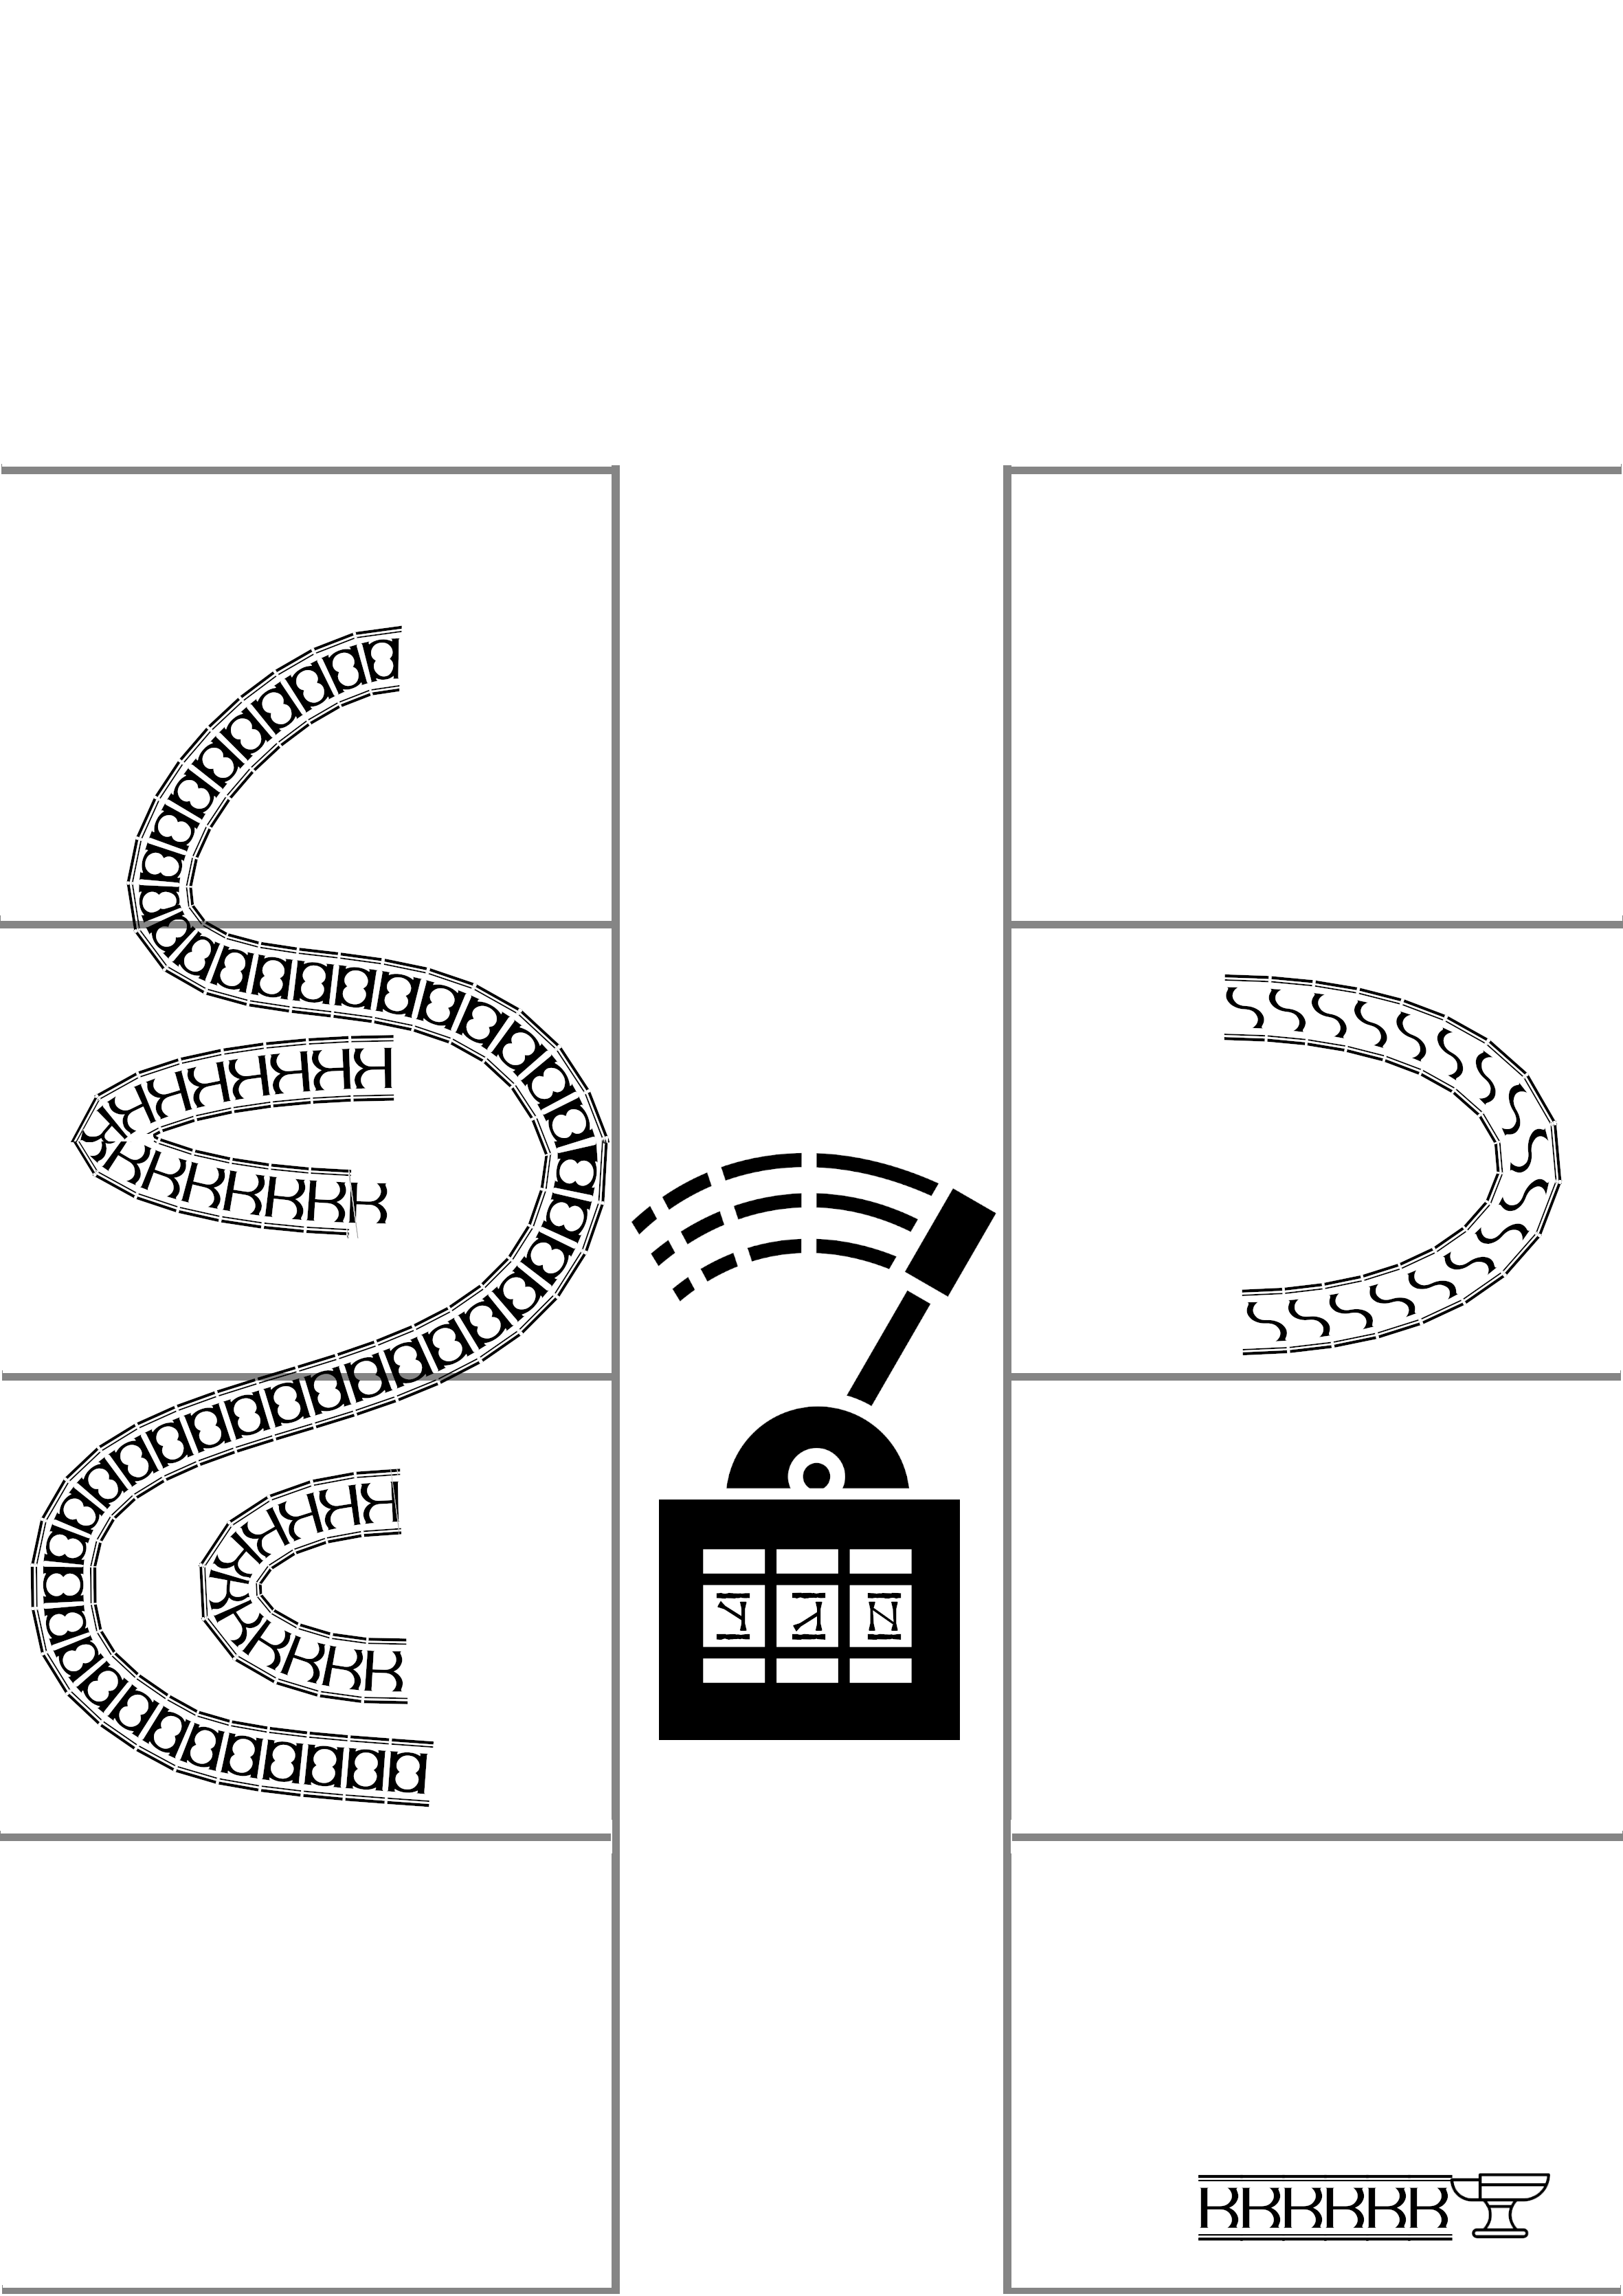
\includegraphics[width=0.95\textwidth]{tor-v.png}}
\newpage
\fbox{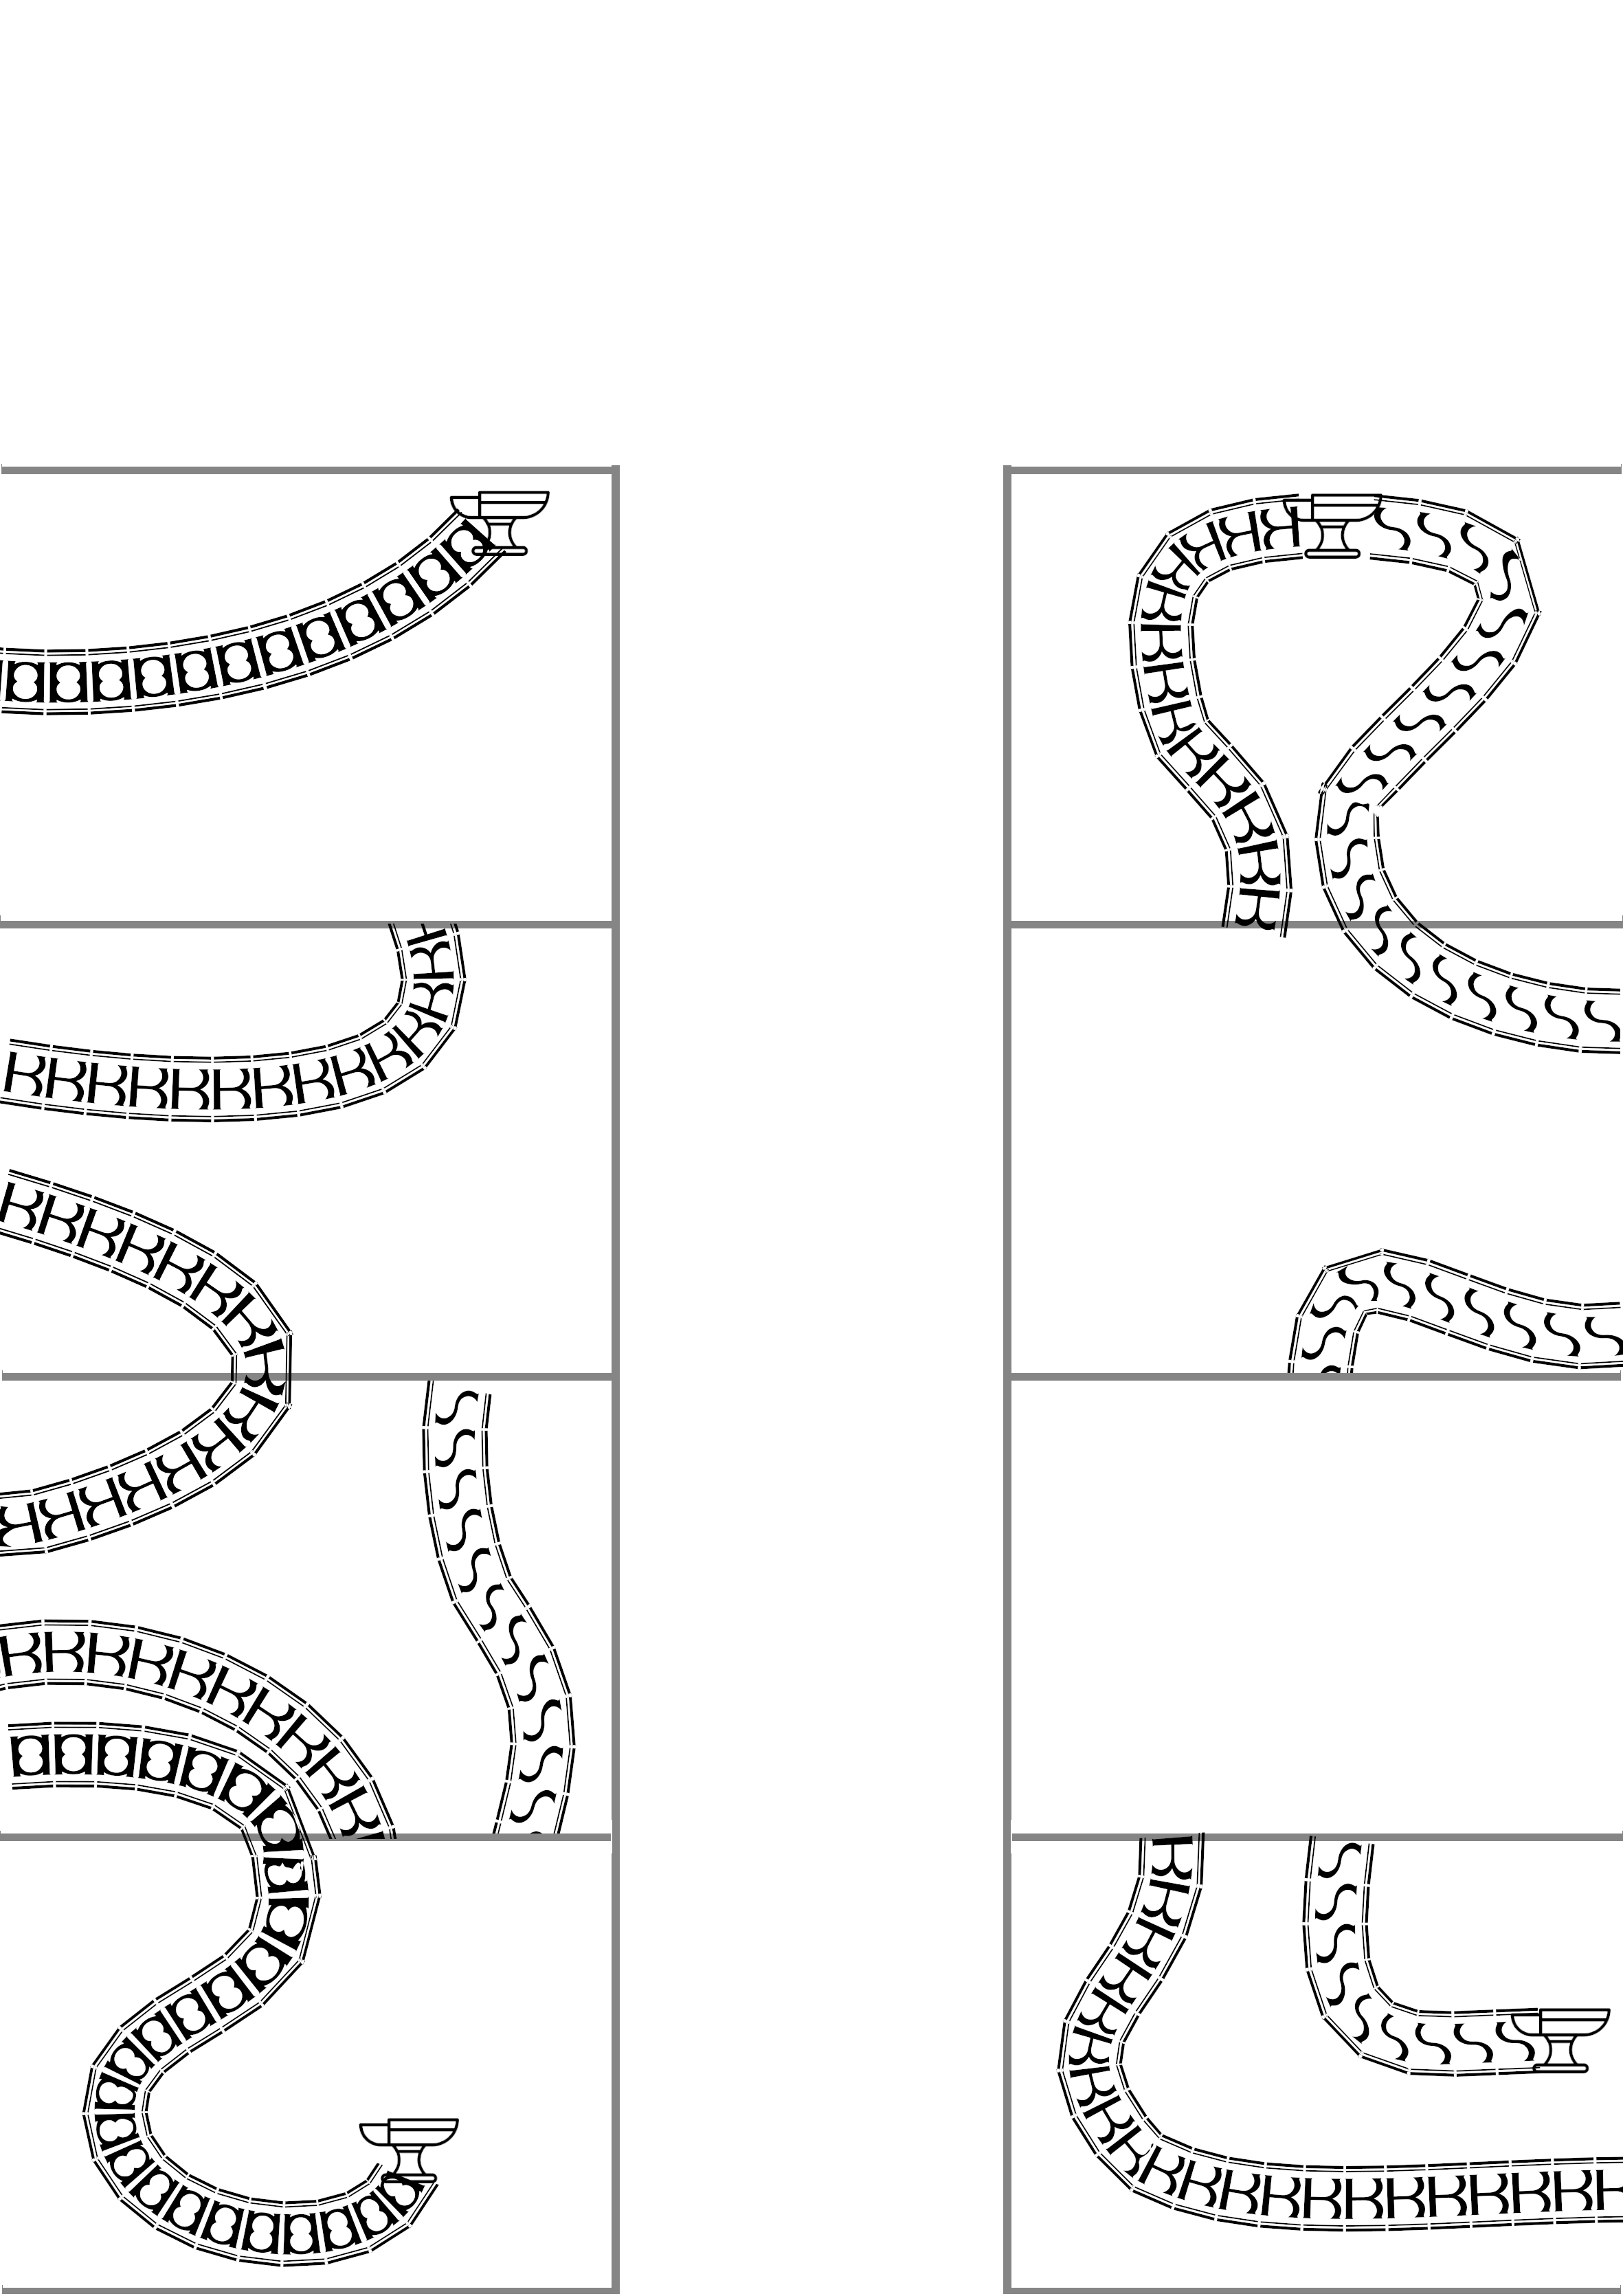
\includegraphics[width=0.95\textwidth]{tor-r.png}}
\newpage

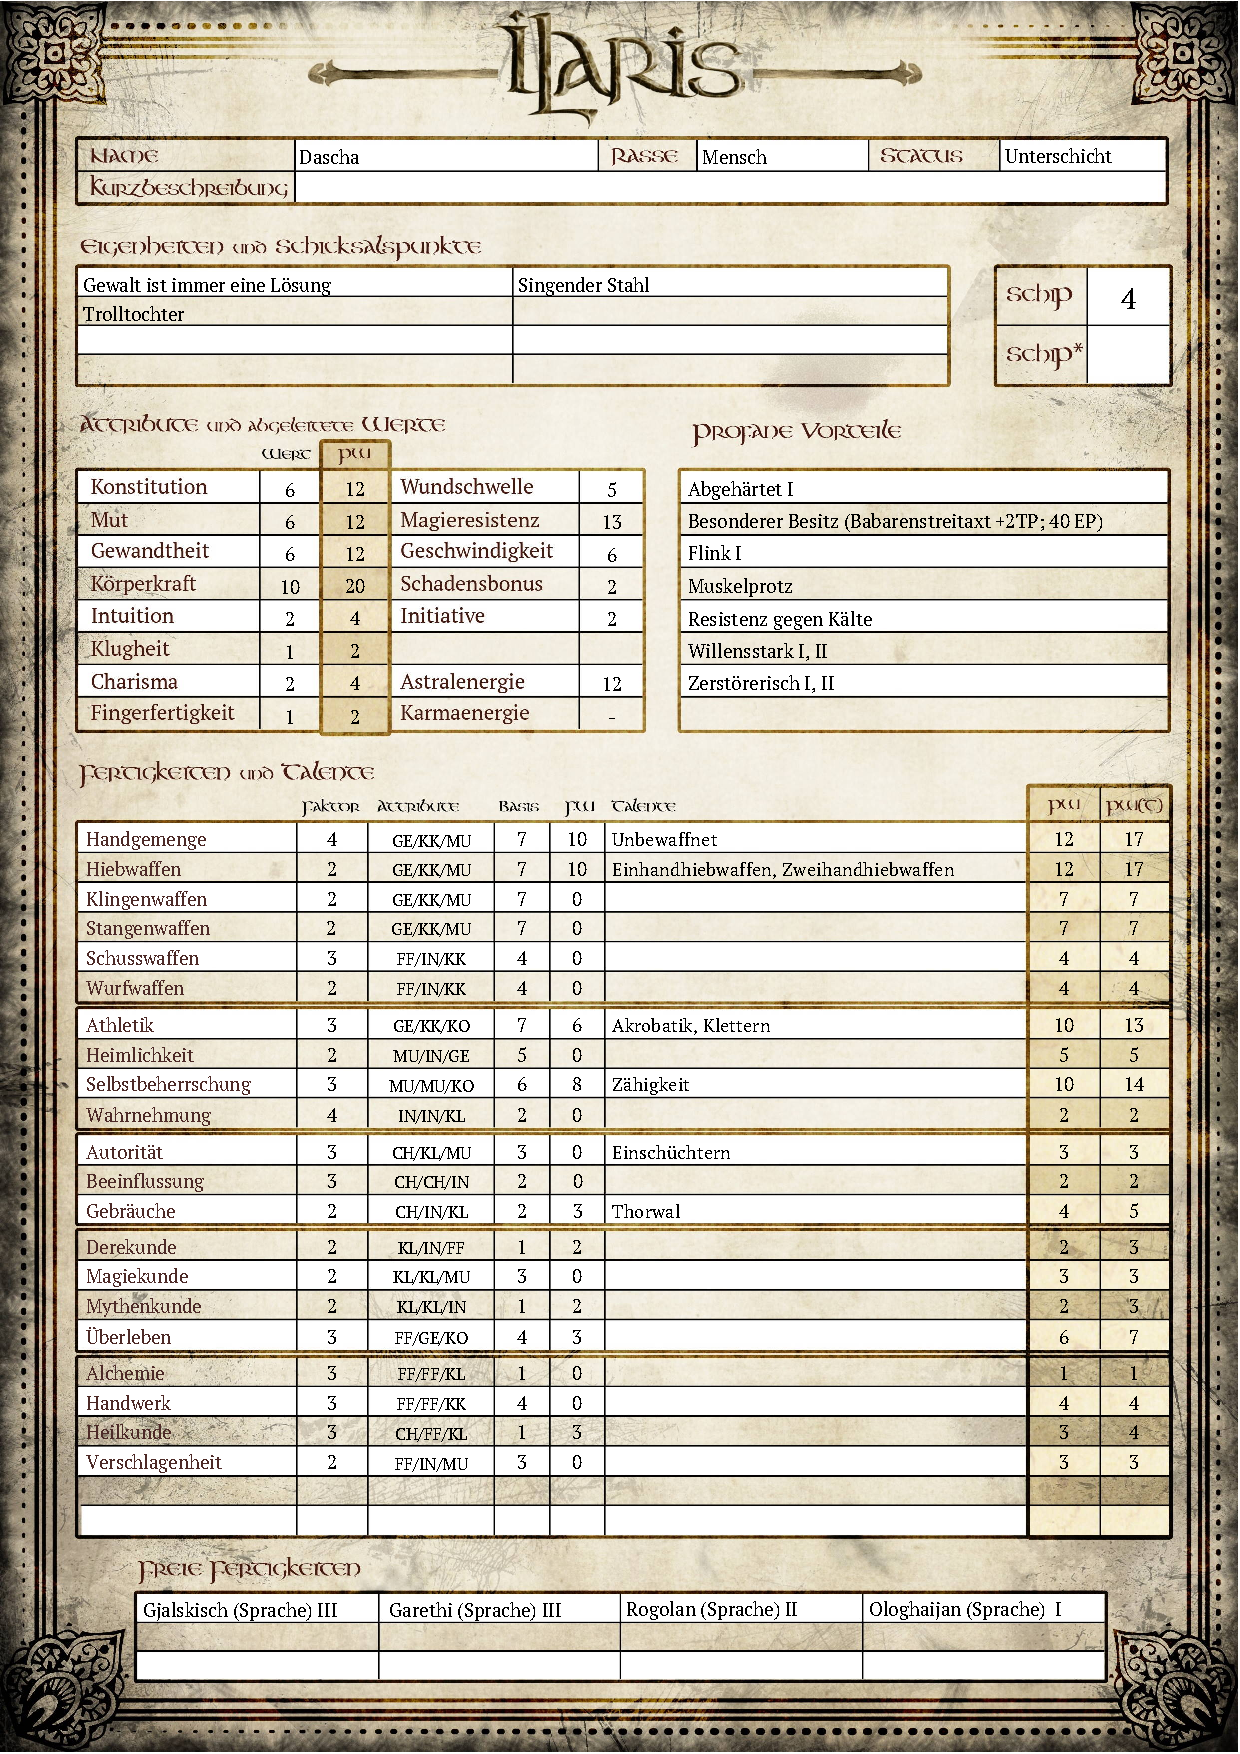
\includepdf[pages=-,addtotoc={1,subsection,1,Charakterbogen Dascha (Tierkriegerin),dascha}]{bergkoenig/pdf/dascha.pdf}
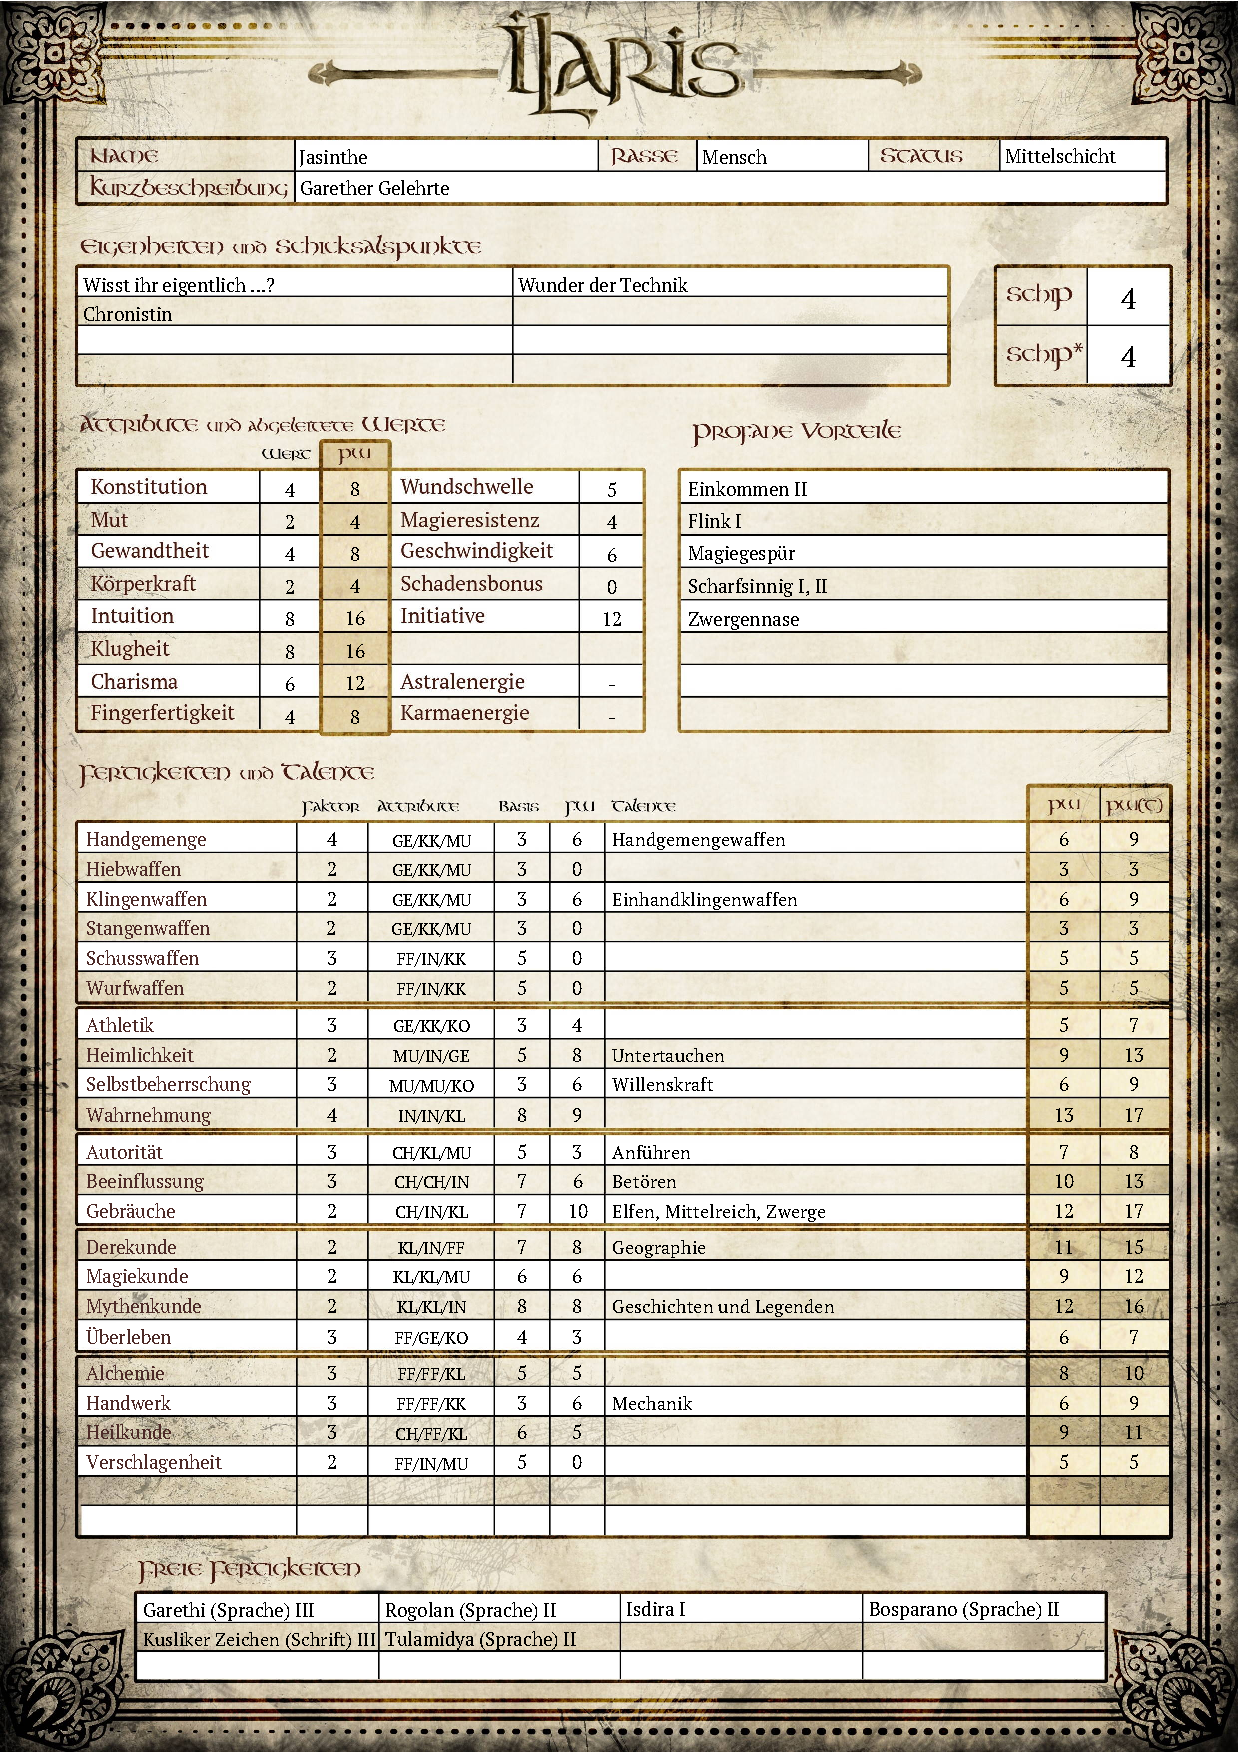
\includepdf[pages=-,addtotoc={1,subsection,1,Charakterbogen Jasinthe (Gelehrte),jasinthe}]{bergkoenig/pdf/jasinthe.pdf}
%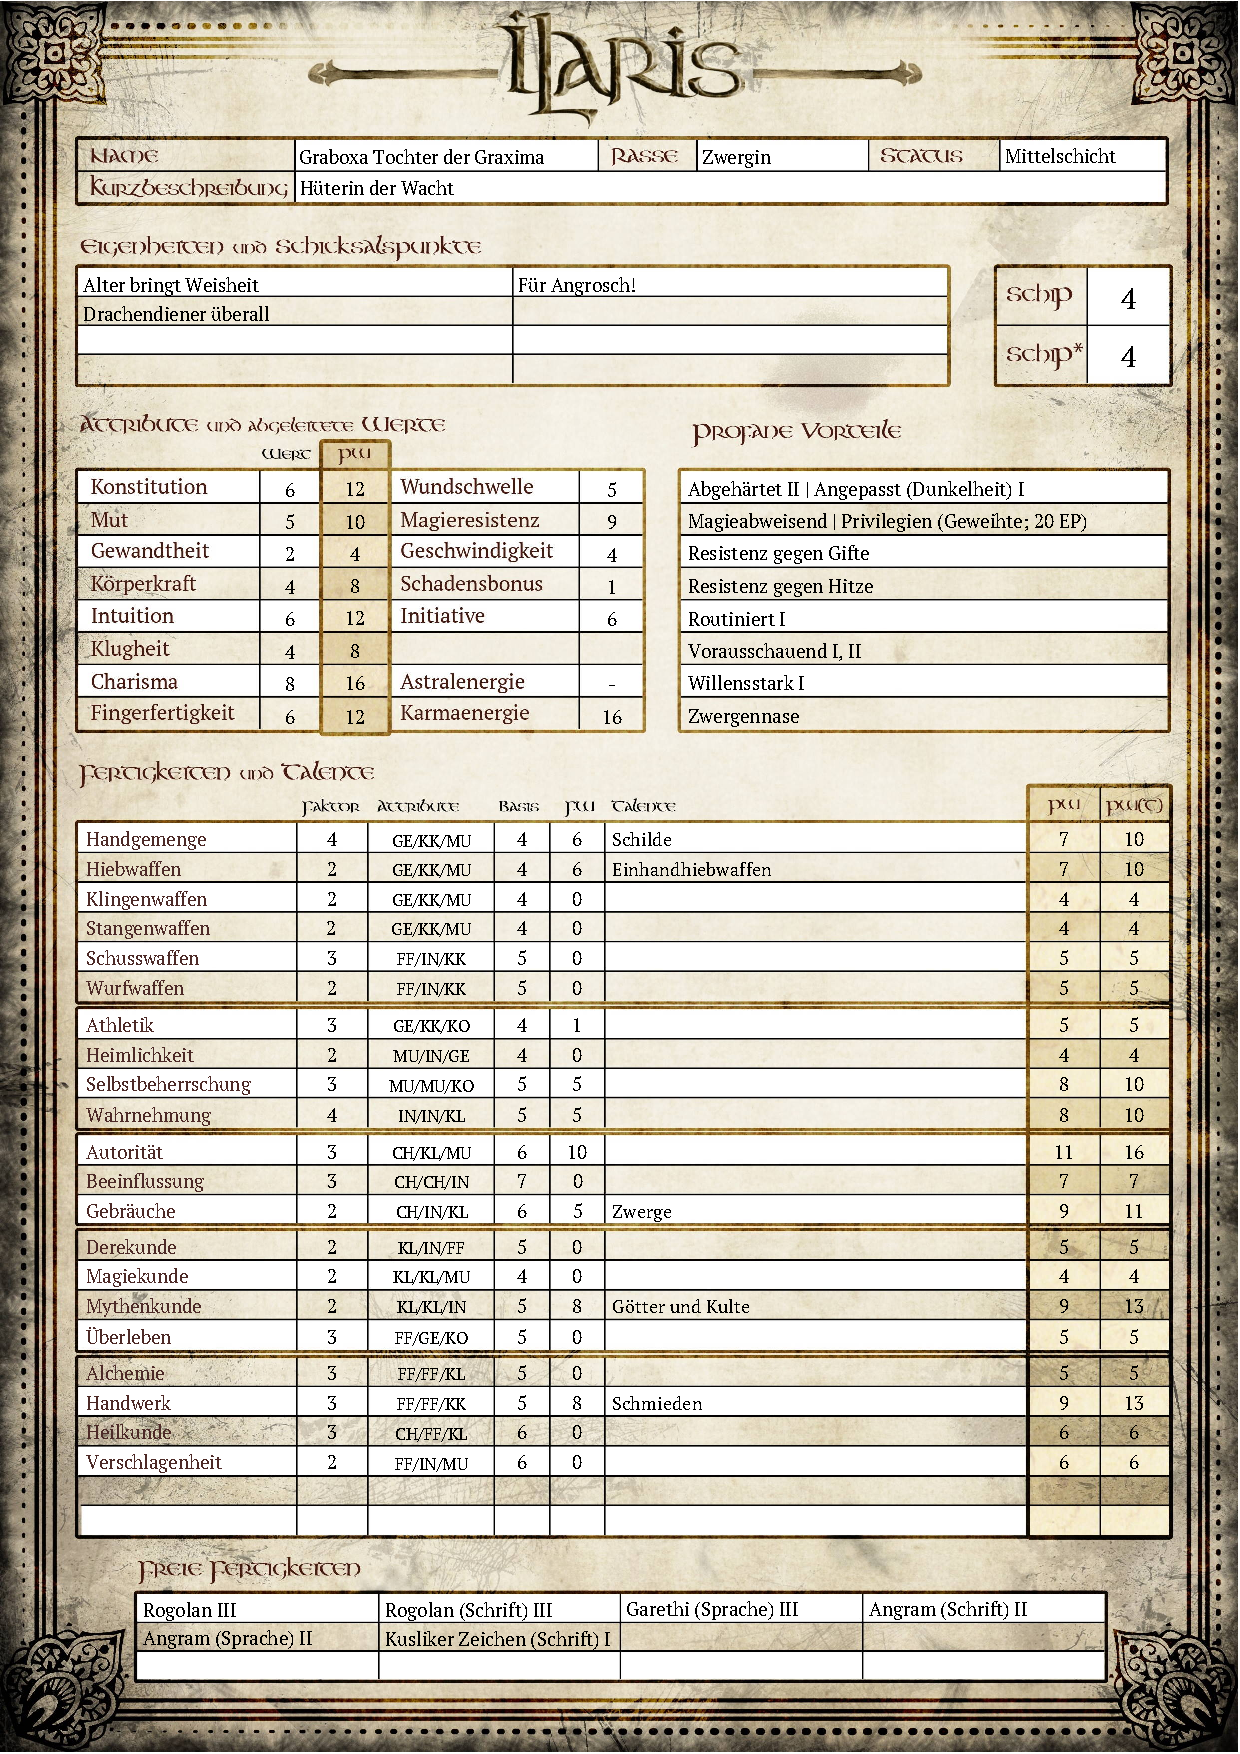
\includepdf[pages=-,addtotoc={1,subsection,1,Charakterbogen Graboxa (Zwergische Angrosch-Geweihte, Hüterin der Wacht),graboxa}]{bergkoenig/pdf/graboxa.pdf}
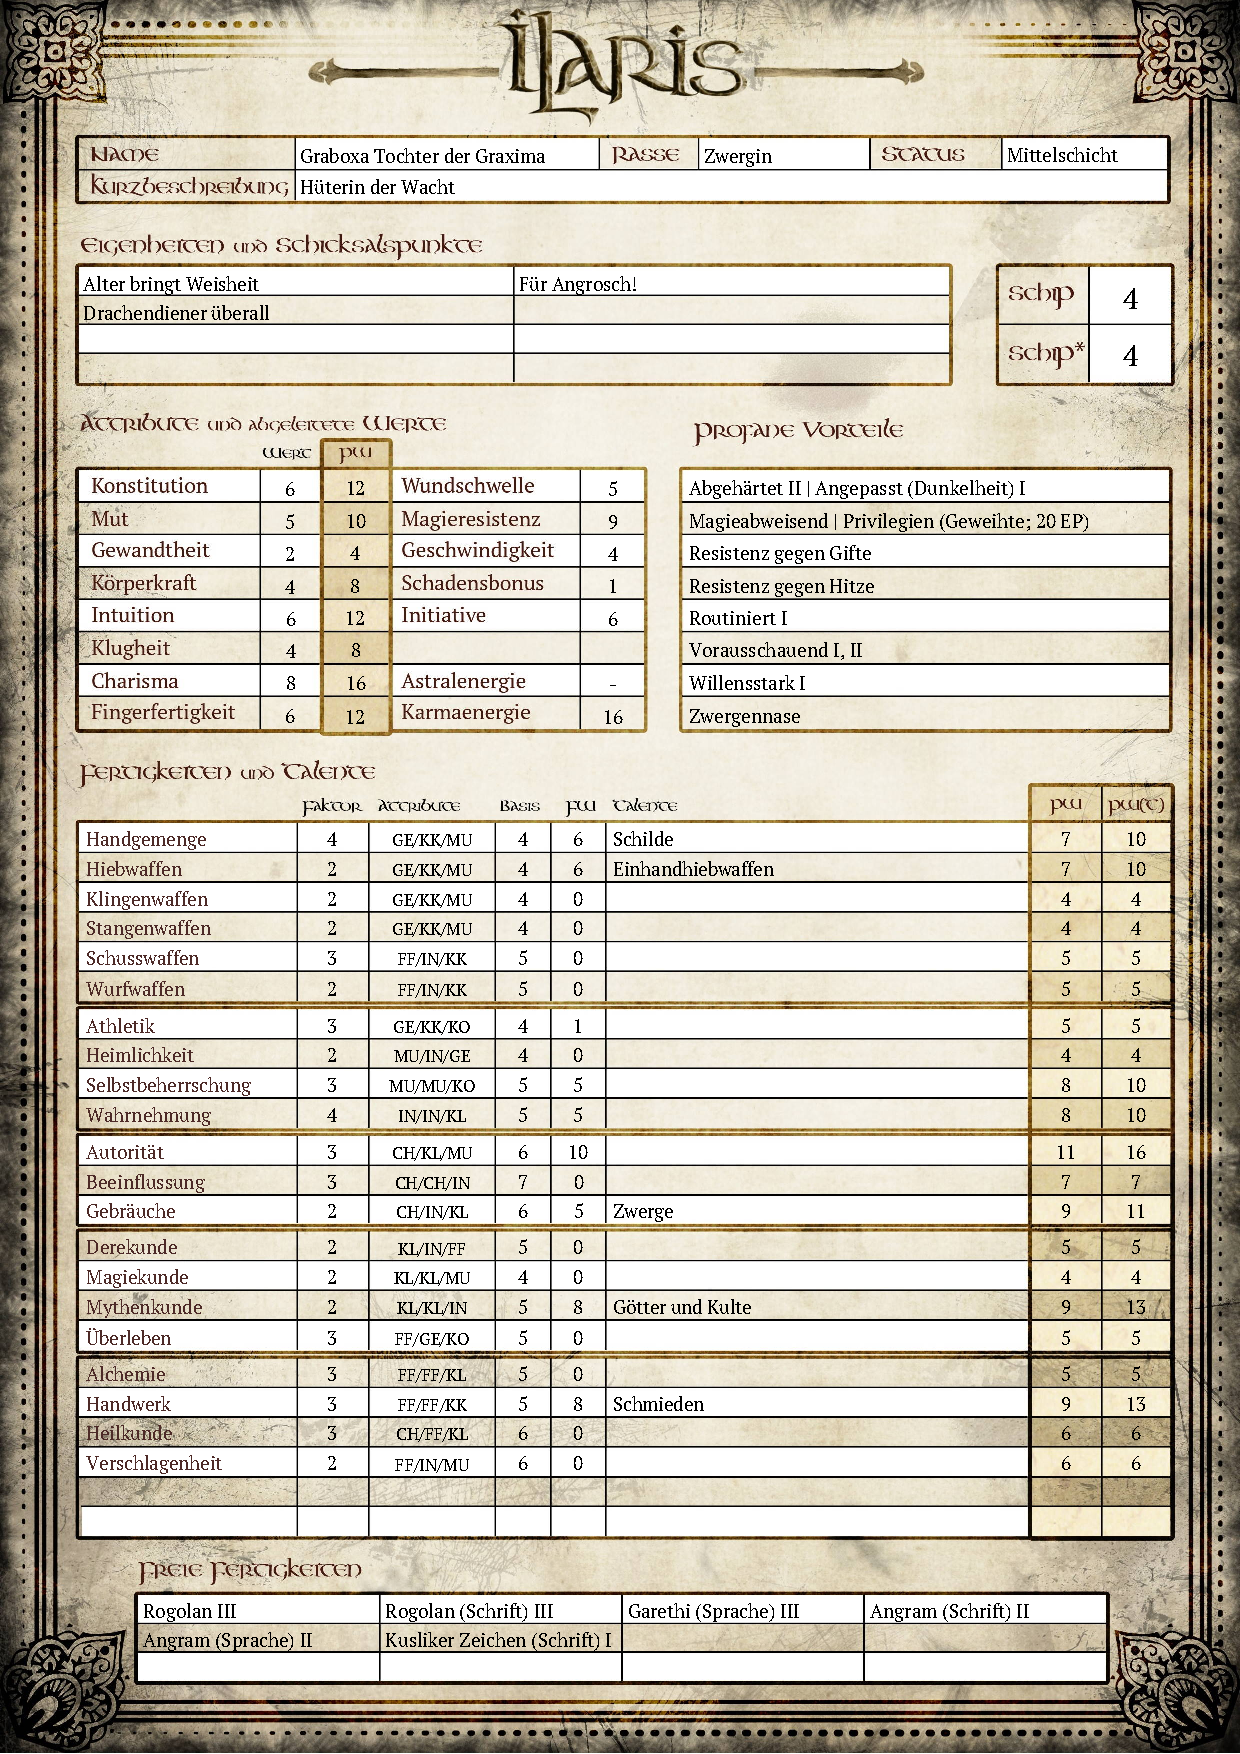
\includepdf[pages=-,addtotoc={1,subsection,1,Charakterbogen Graboxa (Geweihte),graboxa}]{bergkoenig/pdf/Graboxa.pdf}
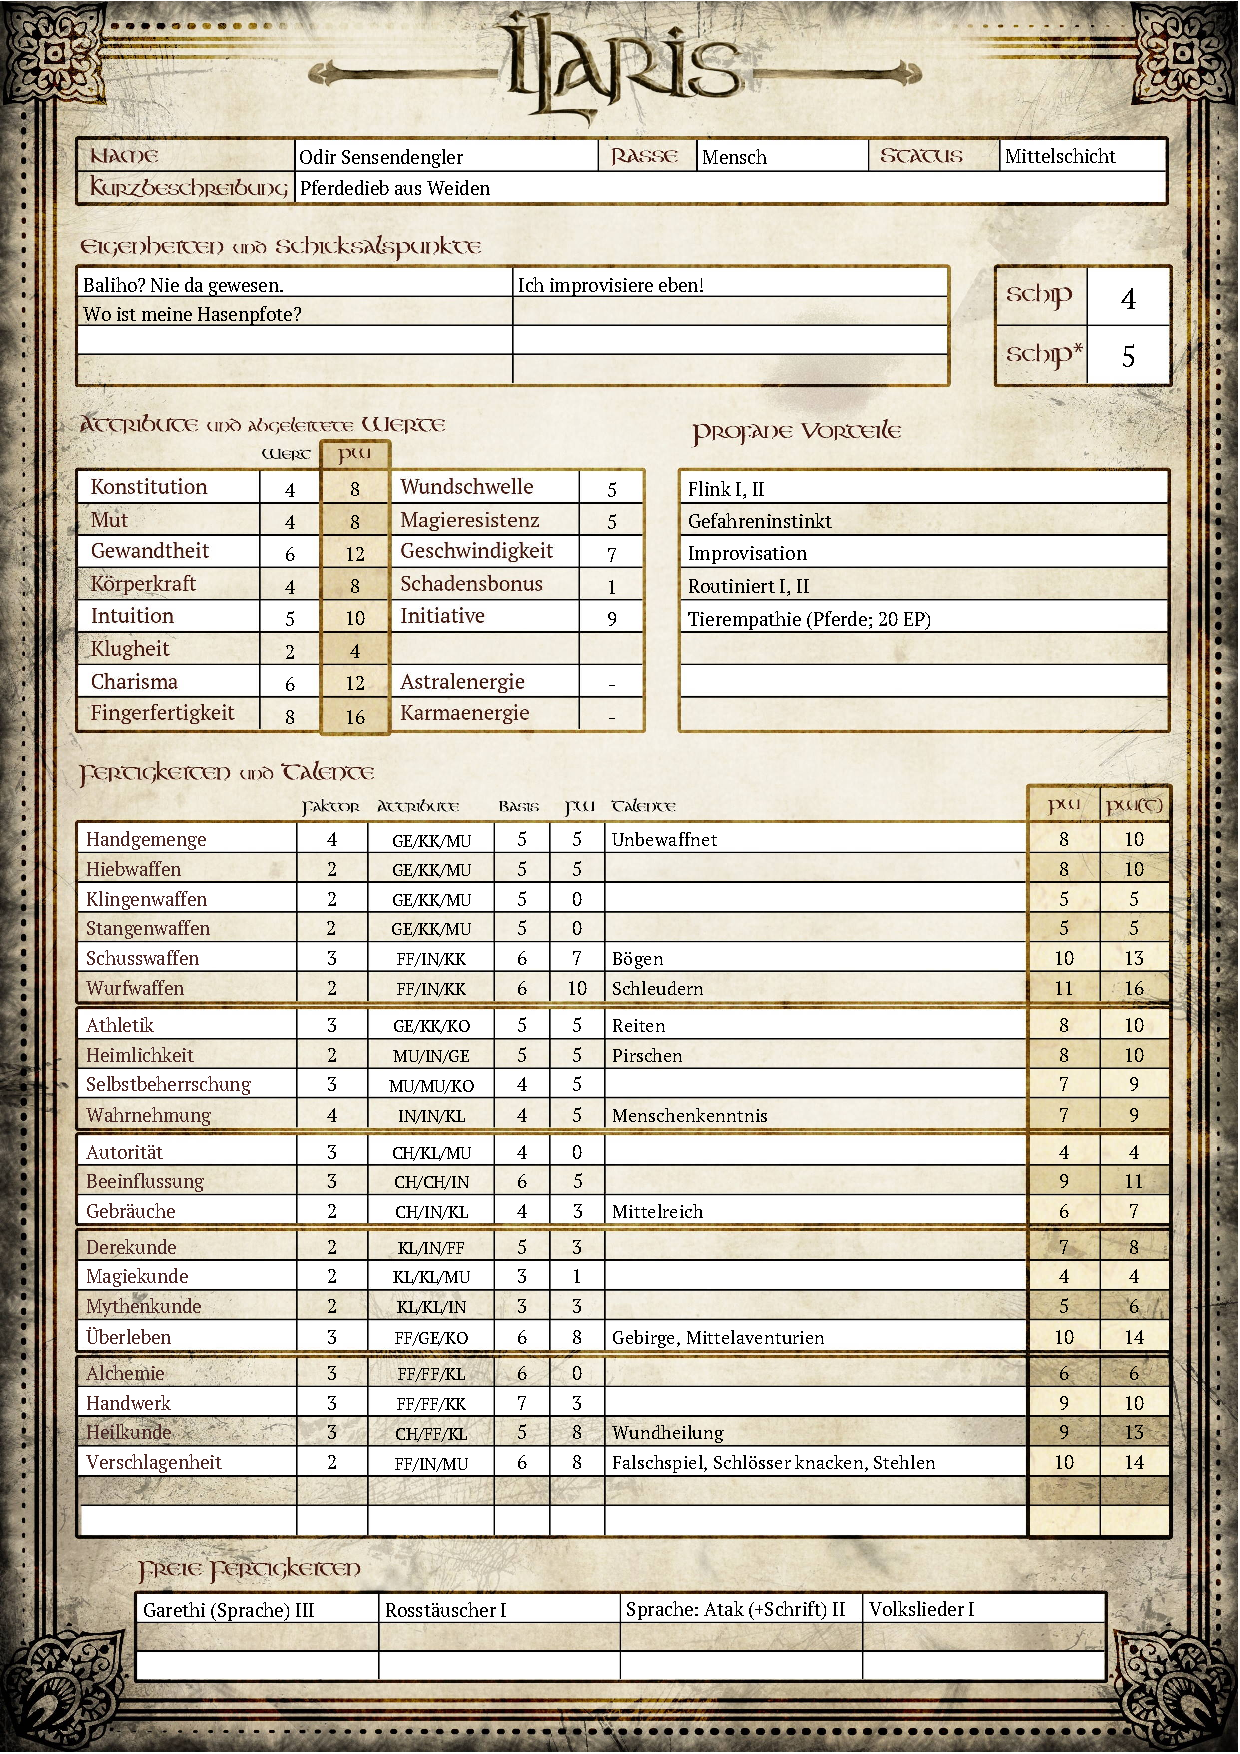
\includepdf[pages=-,addtotoc={1,subsection,1,Charakterbogen Odir (Pferdedieb),odir}]{bergkoenig/pdf/odir_sensendengler.pdf}

\end{document}